\documentclass[11pt]{article}
\usepackage[a4paper,margin=28mm]{geometry}
\usepackage{amsmath,amssymb,amsthm,mathtools,bm}
\usepackage[T1]{fontenc}
\usepackage{lmodern,microtype}
\pdfglyphtounicode{parenleftbig}{0028}
\pdfglyphtounicode{parenrightbig}{0029}
\pdfglyphtounicode{bracketleftbig}{005B}
\pdfglyphtounicode{bracketrightbig}{005D}
\pdfglyphtounicode{parenleftBig}{0028}
\pdfglyphtounicode{parenrightBig}{0029}
\pdfglyphtounicode{parenleftbigg}{0028}
\pdfglyphtounicode{parenrightbigg}{0029}
\pdfglyphtounicode{bracketleftbigg}{005B}
\pdfglyphtounicode{bracketrightbigg}{005D}
\pdfglyphtounicode{braceleftbigg}{007B}
\pdfglyphtounicode{bracerightbigg}{007D}
\pdfgentounicode=1
\usepackage{graphicx,tikz,booktabs,array,longtable}
\usetikzlibrary{arrows.meta,positioning,calc}
\usepackage[numbers,sort&compress]{natbib}
\usepackage[colorlinks=true,linkcolor=blue,citecolor=blue,urlcolor=blue]{hyperref}
\usepackage{bookmark}
\makeatletter
\renewcommand*\l@section[2]{%
  \ifnum\c@tocdepth>\z@
    \addpenalty\@secpenalty\addvspace{1em\@plus\p@}%
    \setlength\@tempdima{2em}%
    \begingroup
      \parindent\z@\rightskip\@pnumwidth\parfillskip-\@pnumwidth
      \leavevmode\bfseries\advance\leftskip\@tempdima\hskip-\leftskip
      #1\nobreak\hfil\nobreak\hb@xt@\@pnumwidth{\hss #2}\par
    \endgroup
  \fi}
\renewcommand*\l@subsection{\@dottedtocline{2}{1.5em}{3.2em}}
\makeatother
\hypersetup{pdftitle={Signed tensor densities and diagram budgets for the Thorp shuffle},pdfauthor={OpenAI}}
\newtheorem{theorem}{Theorem}[section]
\newtheorem{lemma}[theorem]{Lemma}
\newtheorem{proposition}[theorem]{Proposition}
\newtheorem{corollary}[theorem]{Corollary}
\theoremstyle{definition}
\newtheorem{definition}[theorem]{Definition}
\theoremstyle{remark}
\newtheorem{remark}[theorem]{Remark}
\DeclareMathOperator{\Tr}{Tr}
\DeclareMathOperator{\KL}{KL}
\DeclareMathOperator{\Sym}{Sym}
\DeclareMathOperator{\Var}{Var}
\DeclareMathOperator{\Ent}{Ent}
\newcommand{\TV}{\mathrm{TV}}
\newcommand{\HS}{\mathrm{HS}}
\newcommand{\op}{\mathrm{op}}
\newcommand{\E}{\mathbb E}
\newcommand{\PP}{\mathbb P}
\newcommand{\id}{\mathrm{id}}
\newcommand{\eps}{\varepsilon}
\newcommand{\ind}{\mathbf1}
\allowdisplaybreaks[1]
\setlength{\emergencystretch}{2em}
\setcounter{tocdepth}{1}
\title{Signed tensor densities and diagram budgets\\for the Thorp shuffle}
\author{OpenAI}
\date{September 26, 2026}
\begin{document}
\maketitle
\begin{abstract}
We prove that a fixed number of coordinate sweeps of the Thorp shuffle on $2^d$ cards makes the squared $L^2$ distance of the full permutation density from uniform tend to zero as $d\to\infty$. In particular, the total-variation mixing time is $\Theta(d)$ physical shuffles.
\end{abstract}
\section{Introduction}
\label{sec:introduction}
A coordinate sweep visits each coordinate of a binary position once,
independently swapping or retaining the two positions in every coordinate
pair. A single card is uniform after one sweep. The full deck is a more
difficult object: cards share switches, so their joint permutation law can
retain information that every one-card test misses. We bound that
information in every irreducible representation of the symmetric group.
The bounds imply that an absolute number of sweeps suffices for the full
permutation density to converge to uniform in squared $L^2$ distance as
the deck size tends to infinity.

Let $n=2^d$, $d\ge1$, and identify positions with $\{0,1\}^d$.
A sweep first independently swaps or retains every pair in coordinate
direction 1, and then does the same in directions $2,\ldots,d$.
Write $B_n$ for its probability measure and its average action in a
representation. One sweep is $d$ physical Thorp shuffles, after removing
the deterministic rotations of coordinates; Section~\ref{sec:prelim}
gives the exact convention. For $\lambda\vdash n$, let $V_\lambda$ be
the complex Specht module and $D_\lambda=\dim V_\lambda$. Every trace
in this paper is unnormalized.

\subsection*{Prescribed signed occurrences}
The main estimate describes a representation using two kinds of tensor
colors and a remainder. Permuting tensor factors carrying odd colors
introduces a sign; even
colors describe long rows of a Young diagram, and odd colors describe
long columns. The remainder is represented by distinctly marked positions.
Its size enters the bound with an entropy saving that becomes important
when those marks are sparse.

Precisely, let $u+v+l=n$ and let $\alpha\vdash u$, $\beta\vdash v$,
$\gamma\vdash l$. Suppose
\begin{equation}\label{ten:spin:eq:1}
 V_\alpha\otimes V_{\beta^{\mathrm t}}\otimes V_\gamma
 \subseteq\operatorname{Res}^{S_n}_{S_u\times S_v\times S_l}V_\lambda,
\end{equation}
where $\subseteq$ means occurrence, with no multiplicity-one assumption,
and $\beta^{\mathrm t}$ is the transposed partition. Empty factors are
allowed and have dimension one. Define the unnormalized entropy of the
concatenated part lists by
\begin{equation}\label{ten:spin:eq:2}
 F(\alpha,\beta)=\sum_{i:\alpha_i>0}\alpha_i\log\frac{u+v}{\alpha_i}
 +\sum_{j:\beta_j>0}\beta_j\log\frac{u+v}{\beta_j}.
\end{equation}
It is zero if $u+v=0$. All logarithms are natural.

\begin{theorem}[A moment bound for every signed occurrence]
\label{ten:spin:main}\label{s:spin-moment}
For each sufficiently small fixed $\bar\eta>0$, choose a sufficiently
small $\bar\kappa>0$ with $\bar\kappa<\bar\eta/256$. There is an
integer $r\ge1$, depending only on these fixed constants, such that for
every $d\ge1$, every $\lambda\vdash n=2^d$, and every
occurrence~\eqref{ten:spin:eq:1},
\begin{equation}\label{ten:spin:eq:3}
 \log\!\left(D_\lambda\operatorname{Tr}_{V_\lambda}(B_n^*B_n)^r\right)
 \le\eta_d F(\alpha,\beta)+g_n(l),
\end{equation}
where
\[
 \eta_d=\bar\eta\left(1-\frac1{2\sqrt d}\right),\qquad
 \kappa_d=\bar\kappa\left(1-\frac1{2\sqrt d}\right),\qquad
 g_n(l)=\max\{0,\kappa_d l\log n-l\log(n/l)\}.
\]
Set $g_n(0)=0$ and interpret the logarithm of a zero trace as $-\infty$.
\end{theorem}

The occurrence is prescribed, rather than selected by minimizing the
right-hand side. This is useful in the proof itself: a local restriction
supplies particular signed factors and a particular remainder, and the
same theorem applies to those data. The saving $-l\log(n/l)$ is also
essential. The two child bounds retain enough of it to pay for placing
the marks when the children are assembled into the parent rectangle.

\subsection*{The full permutation law}
For a fixed number $L$ of sweeps, let
$f_{d,L}(\sigma)=n!\,B_n^{*L}(\sigma)$ be the density of their
permutation law with respect to the uniform measure $U_{S_n}$.
Let $t_{\mathrm{mix}}(d)$ be the least number of physical shuffles
whose law has total variation distance at most $1/4$ from uniform.

\begin{corollary}[Fixed-sweep convergence of the full deck]
\label{cor:spin-full-deck}
There is an absolute positive integer $L$ such that
\[
 \mathbb E_{U_{S_n}}|f_{d,L}-1|^2\longrightarrow0
 \qquad(d\longrightarrow\infty).
\]
The convergence is uniform over starting orders. Moreover
$t_{\mathrm{mix}}(d)=\Theta(d)$.
\end{corollary}

To obtain the upper bound, choose an occurrence with no remainder and
$F(\alpha,\beta)\le C_0\log D_\lambda$. With $\bar\eta$ sufficiently
small, the theorem then gives a negative power of $D_\lambda$ for the
sweep norm. Summing those powers by finite-group Fourier analysis proves
the corollary. Section~\ref{ten:spin} establishes the required occurrence
and completes this argument. The lower bound comes from the number of
available switch choices: $t$ physical shuffles have support of size at
most $2^{tn/2}$, whereas the uniform law is supported on $n!$ permutations.
Lemma~\ref{lem:support} gives $t_{\mathrm{mix}}(d)\ge2d-O(1)$. The
same fixed-sweep estimate also gives an approximately uniform permutation
sampler whose output coordinates each require only $O(\log n)$ adaptive
queries to shared randomness; see Corollary~\ref{cor:decision-forest}.

\subsection*{The proof mechanism}
There are two sources of contraction. If a representation first appears
on a small number of tracked cards, centering the tuple kernel cancels
every collection of paths with an isolated member. A weighted forest
count bounds the remaining encounters. For the other representations,
split the coordinates into two nearly equal groups. Positions form a
rectangle: the first sub-sweep acts within columns, the second within
rows. The corresponding representation decompositions do not commute,
so the proof must bound the angle between their tensor type spaces.

The angle estimate uses a positive matrix of trace one on each line.
Averaging its tensor powers over the parity-preserving unitary group
dominates the projection to a prescribed signed type. The mean column
density supplies an inverse square root that normalizes all the cells
in a row. The resulting one-cell factors have mean at most one on the
complete rectangle. Removing $l$ cells costs at most $e^l$, while the
global type retains its entropy saving. Section~\ref{sec:static} proves
this comparison, including the local carrier dimensions, before any
moment induction is used.

Distinct marks supply the other local input. As Figure~\ref{fig:marked-grid}
shows, a row move followed by a column move can return a named point
to its initial cell only if both moves fix that point. The trace therefore restricts group-algebra
coefficients to a pointwise stabilizer. This restriction is positive,
and its exact regular-trace factor is the reciprocal of a falling
factorial. Summing mark placements retains the entropy term needed by
the parent bound.

\begin{figure}[t]
\centering
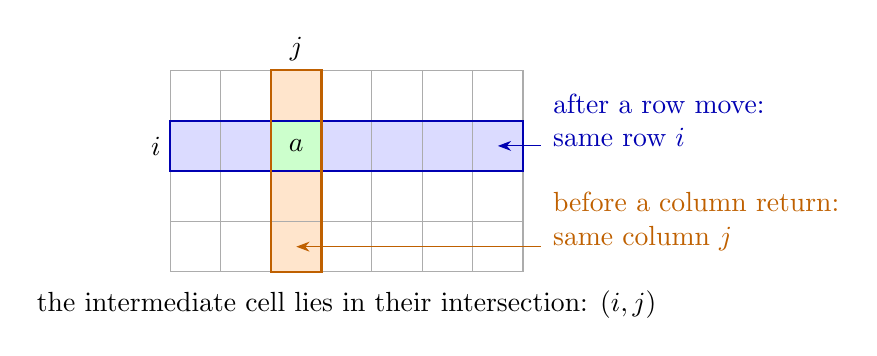
\begin{tikzpicture}[x=.64cm,y=.64cm]
\fill[blue!14] (0,2) rectangle (7,3);
\fill[orange!20] (2,0) rectangle (3,4);
\fill[green!20!white] (2,2) rectangle (3,3);
\draw[step=1,gray!65] (0,0) grid (7,4);
\draw[blue!70!black,thick] (0,2) rectangle (7,3);
\draw[orange!75!black,thick] (2,0) rectangle (3,4);
\node at (2.5,2.5) {$a$};
\node[left] at (0,2.5) {$i$};
\node[above] at (2.5,4) {$j$};
\node[blue!70!black,anchor=west,align=left] at (7.4,3)
  {after a row move:\\same row $i$};
\node[orange!75!black,anchor=west,align=left] at (7.4,1)
  {before a column return:\\same column $j$};
\draw[blue!70!black,-{Stealth}] (7.35,2.5)--(6.5,2.5);
\draw[orange!75!black,-{Stealth}] (7.35,.5)--(2.5,.5);
\node[align=center] at (3.5,-.65)
  {the intermediate cell lies in their intersection: $(i,j)$};
\end{tikzpicture}

\caption{One distinct mark initially occupies cell $(i,j)$ in this
schematic rectangle. After a row move its intermediate location lies
in the highlighted row; a column move can return it to $(i,j)$ only
from the highlighted column. Their intersection is the initial cell.
The same argument for every distinct label forces both moves to fix
all marks. Unmarked cells carry signed tensor factors.}
\label{fig:marked-grid}
\end{figure}

\subsection*{History and mathematical background}
The Thorp shuffle arose in the study of shuffling procedures associated
with Faro~\cite{Thorp1973}. Its simple local rule long resisted a
full-deck mixing analysis. For $n=2^d$, Morris's first polynomial
bound was $O(d^{44})$, using the chameleon process and evolving
sets~\cite{Morris2008}; Montenegro and Tetali improved this to
$O(d^{29})$ through spectral-profile and evolving-set
estimates~\cite[Section~6.4]{MontenegroTetali2006}.
Using entropy contraction, Morris later proved an $O((\log n)^4)$ bound for all even deck
sizes~\cite{Morris2009}, followed by $O(d^3)$ for power-of-two
decks~\cite{Morris2013}. All these bounds count physical shuffles,
rather than sweeps of $d$ coordinate layers. Corollary~\ref{cor:spin-full-deck}
gives $O(d)$ physical shuffles and convergence of the full permutation
density in squared $L^2$, with the matching order supplied by the
support lower bound.

Partial permutation laws are also central to the cryptographic study
of Thorp shuffling~\cite{mrs,MorrisRogawayStegers2018}. Such results
can track many cards: Czumaj and V\"ocking proved an
$O((\log n)^2)$ bound for the joint positions of any fixed fraction
$cn$ of the cards, where $0<c<1$, using non-Markovian
coupling~\cite{CzumajVocking2014}. The distinction here is the passage
to the joint law of all $n$ cards. The signed representation estimates
retain that complete permutation information instead of selecting a
prescribed family of card marginals.

We use the classical branching and Littlewood--Richardson rules, the
hook-length formula, and ordinary Schur--Weyl
duality~\cite{James1978,Sagan2001,Stanley1999,etingof,VershikOkounkov2005}.
Signed tensor and hook combinatorics have their representation-theoretic
ancestry in Berele and Regev; hook-Schur formulas and their positive
tableau descriptions are also developed by Orellana and Zabrocki and
by Mason and Niese~\cite{BereleRegev1987,orellana-zabrocki2000,mason-niese2016}.
Our decomposition uses ordinary Schur--Weyl duality on the two parity
classes, a sign twist, and induction. The density comparisons and the
budget estimates are proved here.

The passage from Fourier estimates to total variation is the
finite-group method of Diaconis and
Shahshahani~\cite{DiaconisShahshahani1981}. Their random-transposition
law is central. A coordinate sweep is generally nonnormal: its product
with its adjoint need not equal the product in the opposite order.
We use the Araki--Lieb--Thirring inequality for positive
matrices~\cite{araki1990,audenaert2007} to recurse on moments, and
Schatten H\"older to pass to repeated forward sweeps.

\subsection*{The later bounds}
Theorem~\ref{s:spin-moment} and Corollary~\ref{cor:spin-full-deck} are
proved in Section~\ref{ten:spin}. The remainder of the paper studies
what additional information a moment estimate can retain. Some bounds
optimize over signed factors and marks; others keep every prescribed
hook subdiagram, minimize over all subdiagrams, or couple a first-row
defect bound with a row-and-column weight. Their statements differ in
both their optimization domains and their moment exponents.

These later sections also develop distinct mechanisms: lowering
operators give a norm estimate throughout $2\le k\le n/2$;
covariance retains local ranks; a harmonic-tuple coupling gives a
separate sparse estimate; and ordered products of densities provide
another marked-grid proof. They supply alternative routes to the same
mixing order, as well as their stated finer estimates.
Part~\ref{part:refinements} begins with the guide in Section~\ref{s:later-routes}, which
compares these targets and the information each retains.
Section~\ref{s:full-isotypic-section} then provides the common
full-isotypic, positive-mixture, coefficient-integral, and
marked-recurrence tools before the individual arguments begin.

\clearpage
\tableofcontents
\clearpage
\part{The every-occurrence bound}\label{part:every-occurrence}
\section{The physical chain, Fourier norms and dimension estimates}\label{sec:prelim}
This section fixes the common normalization. Every later passage from a sweep estimate to mixing uses physical time measured here.

\subsection{Binary positions and sweep operators}
Number positions by $x=(x_1,\ldots,x_d)\in\mathbb F_2^d$, most significant bit first. One shuffle sends
\[
 x\longmapsto(x_2,\ldots,x_d,x_1+\xi_{x_2,\ldots,x_d}),
\]
where the $2^{d-1}$ bits $\xi$ are independent and fair. Write $R$ for the cyclic rotation and $h_t$ for the pair switches at physical time $t$, so the time-$t$ permutation is $Rh_t\cdots Rh_1$. Factoring out $R^t$ conjugates the switches into the successive coordinate directions. This deterministic left multiplication preserves distance to uniform. At time $d$, $R^d=I$, and one sweep has exactly the law of $d$ physical shuffles. Write $q_d$ for the law of one physical shuffle and
$U_{S_n}$ for the uniform measure. We use
\[
 t_{\mathrm{mix}}(d)=\min\{t\ge0:
       \|q_d^{*t}-U_{S_n}\|_{\mathrm{TV}}\le1/4\}.
\]
Translation by the starting permutation shows that this is also the
worst-initial-state mixing time.

Permutations send each input position to its output. A product $gh$ applies $h$ first. For measures, $\mu*\nu$ denotes the law of $gh$ for independent $g\sim\mu,h\sim\nu$. In a unitary representation $\rho_\lambda$, define
\[
 \widehat\mu(\lambda)=\sum_g\mu(g)\rho_\lambda(g),
 \qquad\widehat{\mu*\nu}=\widehat\mu\,\widehat\nu.
\]
A fair switch layer averages the subgroup generated by its disjoint transpositions, and hence is an orthogonal projection $\Pi_i$. With chronological coordinate order $1,\ldots,d$, put
\[
 B_n=\Pi_d\cdots\Pi_1,\qquad Q_n=B_n^*B_n,
 \qquad n=2^d.
\]
The layered switching network for this product is the butterfly network.
In later sections, a butterfly means this same complete coordinate sweep,
both as a random permutation and as its average operator.
\begin{lemma}[Annihilated shapes]\label{lem:annihilation}
The sign representation is annihilated by every nonempty fair layer. Every irreducible of $S_n$ indexed by a shape with more than $n/2$ rows is annihilated by a sweep.
\end{lemma}\begin{proof}
The sign average contains a fair transposition. For the second assertion, by Young's rule, the permutation module induced from the trivial representation of $(S_2)^{n/2}$ has only shapes dominating $(2^{n/2})$, hence at most $n/2$ rows.
\end{proof}

\begin{lemma}[Finite-size norm gap]\label{lem:finitegap}
For every fixed dyadic $n\ge2$, $\|B_n(\lambda)\|_{\op}<1$ on every nontrivial irreducible.
\end{lemma}
\begin{proof}
Equality on a unit vector would force equality at every orthogonal projection in the product. The vector would be fixed by all coordinate-pair transpositions. The edges of the cube form a connected graph, and its edge transpositions generate $S_n$, contradicting nontrivial irreducibility.
\end{proof}


\begin{lemma}[Support obstruction]\label{lem:support}\label{ten:support}
For every integer $t\ge0$,
\[
 \|q_d^{*t}-U_{S_n}\|_{\TV}\ge1-2^{tn/2}/n!.
\]
Consequently $t_{\mathrm{mix}}(d)\ge\lceil(2/n)\log_2(3n!/4)\rceil=2d-O(1)$.
\end{lemma}
\begin{proof}
At most $2^{tn/2}$ coin strings are available, so the law is supported on at most that many permutations. Comparing this support set with its uniform mass proves the first assertion. Distance at most $1/4$ requires support mass at least $3/4$, giving the exact integer lower bound. Stirling's formula gives the final expression and, before the integer
rounding, the sharper expansion
$\frac2n\log_2(3n!/4)=2d-2\log_2 e+o(1)$.
For $t\le d$, the support fraction is at most $n^{n/2}/n!=o(1)$,
so the distance is $1-o(1)$.
\end{proof}

\subsection{Plancherel and powers of a nonnormal sweep}
All matrix traces and Schatten norms are unnormalized. Thus $\|A\|_{S^p}^p=\Tr|A|^p$, with $S^2=\HS$ and $S^\infty=\op$. If $D_\lambda$ is the irreducible dimension, finite-group orthogonality gives
\[
 |G|\sum_g|\mu(g)|^2=\sum_\lambda D_\lambda\|\widehat\mu(\lambda)\|_{\HS}^2.
\]
It applies to signed measures and subprobabilities as well as probabilities. For a measure $v$ of mass $m$,
\begin{equation}\label{eq:plancherel}
 \|v-mU_G\|_1^2\le
 \sum_{\lambda\ne\mathbf1}D_\lambda\|\widehat v(\lambda)\|_{\HS}^2.
\end{equation}
For a probability the left side is $4\|v-U_G\|_{\TV}^2$. If $0\le v\le\mu$ and $\mu$ is a probability, then
\begin{equation}\label{eq:lostmass}
 \|\mu-U_G\|_{\TV}\le1-m+\tfrac12\|v-mU_G\|_1.
\end{equation}
Both follow from Cauchy--Schwarz and the triangle inequality, respectively.

\begin{lemma}[Safe use of sweep powers]\label{lem:schatten}
For integers $r\ge s\ge1$ and any matrix $T$, setting $Q=T^*T$,
\[
 \|T^r\|_{\HS}^2\le\|Q\|_{\op}^{r-s}\Tr Q^s.
\]
\end{lemma}
\begin{proof}
Schatten H\"older gives $\|T^s\|_{\HS}\le\|T\|_{S^{2s}}^s$, and multiplying the remaining $r-s$ factors costs at most $\|T\|_{\op}^{r-s}$. Squaring proves the claim. No normality of $T$ is used.
\end{proof}

\subsection{Injection multiplicities and inverse-degree sums}
We use the standard indexing of complex irreducibles of $S_n$ by partitions $\lambda\vdash n$, with $D_\lambda=f^\lambda$ equal to the number of standard tableaux~\cite{Sagan2001,Stanley1999}. Write $k=n-\lambda_1$ and $\bar\lambda=(\lambda_2,\lambda_3,\ldots)$. Young branching and Frobenius reciprocity show that the representation on ordered distinct $r$-tuples contains $\lambda$ with multiplicity
\[
 f^{\lambda/(n-r)}.
\]
At $r=k$ this is $f^{\bar\lambda}$, and $\lambda$ does not occur on fewer slots. If $k\le r\le n-k$, the remaining first-row boxes are separated from the tail, giving
\begin{equation}\label{eq:tuplemultiplicity}
 m_\lambda(r)=\binom rk f^{\bar\lambda},\qquad
 D_\lambda\le\binom nk f^{\bar\lambda}.
\end{equation}
The inequality follows by choosing the entries below the first row and forgetting cross-row tableau constraints.
The same hook formula gives the useful quantitative refinement
\begin{equation}\label{eq:near-row-hooks}
 D_\lambda\ge\binom nk f^{\bar\lambda}
       \exp\left(-\frac{k}{n-2k+1}\right)
 \qquad(0\le k\le n/2).
\end{equation}
Indeed the hook inflation along the top row, relative to $(n-k)!$, is
\[
 \prod_{j\le\lambda_2}\left(1+
   \frac{\lambda'_j-1}{n-k-j+1}\right).
\]
The denominators are at least $n-2k+1$ and
$\sum_j(\lambda'_j-1)=k$. Taking logarithms bounds this product by
$\exp(k/(n-2k+1))$. The remaining hooks are exactly those of
$\bar\lambda$. In particular for $k\le.14n$ the loss is $\exp(O(k/n))$,
which also supplies the weaker $\exp(O(k\log n/n+k/n))$ loss when that
form is convenient.


The inverse-degree convergence below is the case $s=1$ of the stronger estimate of Liebeck and Shalev~\cite[Theorem~2.6]{liebeck-shalev2004}. We include an elementary proof together with the pointwise bound needed later. These estimates specify which negative dimension powers are available to the different proofs.
\begin{lemma}[Degree sums]\label{lem:degrees}
Uniformly in $n$, $\sum_{\lambda\vdash n}D_\lambda^{-1}$ is bounded, and
\[
 \sum_{\lambda\ne(n),(1^n)}D_\lambda^{-1}\longrightarrow0.
\]
If $\ell=n-\max(\lambda_1,\lambda'_1)$, then
\[
 \log D_\lambda\ge(\log2)\sqrt\ell/2,
 \qquad \sup_n\sum_{\lambda\vdash n}D_\lambda^{-32}<\infty.
\]
\end{lemma}
\begin{proof}
Transpose if necessary so that the first row has length $r=\max(\lambda_1,\lambda'_1)$. If $r\le n/8$, the hook formula gives $D_\lambda\ge n!/(2r)^n$, exponential in $n$. If $n/8<r\le3n/4$, retain the first row and $\lfloor r/4\rfloor$ further boxes. Their tableaux extend to the whole diagram. A first row of length $r$ and a tail of size $j\le r$ have at least
\[
 \binom{r+j}{j}\frac{r-j+1}{r+1}
\]
tableaux: ballot interleavings of the first row with any fixed standard order of the tail respect all column inequalities. This is exponential in $n$ in the present range. There are $\exp(O(\sqrt n))$ partitions, so these ranges contribute $o(1)$ to the inverse-degree sum. If $r>3n/4$, write $j=n-r$. The same ballot bound is at least a fixed multiple of $\binom nj$. There are at most $2p(j)$ possible shapes up to transpose, and $\binom nj\ge4^j$ for $j<n/4$. Since $p(j)=\exp(O(\sqrt j))$ and each fixed positive $j$ gives a divergent binomial coefficient, dominated convergence proves the first assertion.

For the square-root estimate, put $b=\lambda_2$ and $h=\lambda'_1$, so $b(h-1)\ge\ell$. If $h-1\ge\sqrt\ell$, a hook with row and column length $h$ has at least $2^{h-1}$ tableaux. Otherwise $b\ge\sqrt\ell$ and the two-row rectangle of width $b$ has the Catalan number of tableaux, at least $2^{b-1}$. Subdiagram tableaux extend; handling $\ell=0$ separately proves the displayed bound. Finally $p(j)\le e^{3\sqrt j}$ follows by evaluating the partition generating product at $e^{-1/\sqrt j}$. Summing $2e^{3\sqrt\ell}e^{-16(\log2)\sqrt\ell}$ proves the inverse-32 bound.
\end{proof}

\section{Signed densities and pointwise stabilizers}\label{sec:static}\label{ten:guide}
We now prove the two comparisons needed by the first moment induction. The density estimate retains both the global entropy and all local carrier factors. The stabilizer estimate retains the exact index of the subgroup. Neither argument uses a sweep moment bound.


Let $E$ and $O$ be orthogonal copies of $\mathbb C^q$, with $q\ge1$,
and set $V=E\oplus O$. On $V^{\otimes p}$ a permutation acts by
permuting factors and multiplying by the sign of its permutation of the
odd factors. A density is called even if it is positive, has trace one,
and preserves $E$ and $O$. Put $G_q=U(E)\times U(O)$.
For partitions $a,b$ with at most $q$ parts and $|a|+|b|=p$, define
\[
 F(a,b)=p\log p-\sum_i a_i\log a_i-\sum_jb_j\log b_j,
 \qquad u(a,b)=\dim\mathcal U_a\dim\mathcal U_b,
\]
where $\mathcal U_a,\mathcal U_b$ are the ordinary polynomial unitary
representations. Zero summands are omitted; $F(\varnothing,\varnothing)=0$
and $u(\varnothing,\varnothing)=1$. All traces below are unnormalized.
Throughout this paper, Haar measures on compact groups are normalized to
probability. We use compact matrix-coefficient orthogonality in the form
of Morel~\cite[Theorem IV.3.8(i)--(ii), pp.~84--85]{Morel2018}.
The $G_q$-isotypic projection $Q_{a,b}$ has range
\begin{equation}
 \mathcal M_{a,b}\otimes\mathcal U_a\otimes\mathcal U_b,
 \qquad
 \mathcal M_{a,b}=
 \operatorname{Ind}_{S_{|a|}\times S_{|b|}}^{S_p}
          (V_a\otimes V_{b^t}).
 \label{eq:signed-sector-decomposition}
\end{equation}
Indeed, first fix the even sites, apply ordinary Schur--Weyl duality~\cite[Theorem 4.57 and Corollary 4.59]{etingof}
separately to the two kinds of sites, twist the odd symmetric-group
factor by sign, and then sum over allocations of the even sites.

\begin{lemma}[Density domination of a signed spin type]
\label{lem:signed-type-density}
For every such $(a,b)$ there is a probability distribution on even
densities $R$ such that
\begin{equation}
 Q_{a,b}\preceq e^{F(a,b)}u(a,b)\,\mathbb E R^{\otimes p}.
 \label{eq:signed-type-density-exact}
\end{equation}
For every even density $T$ and every type $(a,b)$,
\begin{equation}
 \|T^{\otimes p}Q_{a,b}\|_{\rm op}\le e^{-F(a,b)}.
 \label{eq:signed-global-density-upper}
\end{equation}
Moreover $u(a,b)\le(p+1)^{q(q-1)}$.

For arbitrary parity dimensions, the upper bound has the following
carrier form. Let
$E_+=\mathbb C^{r_+}$ and $E_-=\mathbb C^{r_-}$, for nonnegative integers
$r_+,r_-$, and let $a,b$ have at most $r_+,r_-$ parts,
respectively, with $|a|+|b|=p$. Write $\mathbf S_a(E_+)$ and
$\mathbf S_b(E_-)$ for the ordinary polynomial carriers of highest
weights $a,b$. For a positive parity-preserving matrix $T$ on
$E_+\oplus E_-$, let its induced carrier action be
$\pi_{a,b}(T)=\mathbf S_a(T|_{E_+})\otimes\mathbf S_b(T|_{E_-})$.
With $F(a,b)$ given by the same entropy formula,
\begin{equation}
 \|\pi_{a,b}(T)\|_{\rm op}
 \le (\operatorname{Tr}T)^p e^{-F(a,b)}.
 \label{eq:signed-carrier-density-upper}
\end{equation}
A zero-dimensional factor has the empty partition and contributes
the scalar identity. If $p=0$, then $\pi_{a,b}(T)=1$ and the
right-hand side is interpreted as one, even when $\operatorname{Tr}T=0$.
\end{lemma}
\begin{proof}
For $p=0$ all assertions mean the identity on a one-dimensional space.
For the density domination with $p>0$, take the density with
eigenvalues $a_i/p$ on $E$ and $b_j/p$ on $O$, padded with zeroes,
and conjugate it by Haar $G_q$. On the
sector in \eqref{eq:signed-sector-decomposition}, its tensor power is
the identity on $\mathcal M_{a,b}$ times the polynomial action on the
two unitary factors. Haar averaging is scalar on their irreducible
tensor product. Its scalar is the trace of that action divided by
$u(a,b)$. The highest weight contributes the eigenvalue
\[
 \prod_i(a_i/p)^{a_i}\prod_j(b_j/p)^{b_j}=e^{-F(a,b)};
\]
therefore the scalar is at least $e^{-F(a,b)}/u(a,b)$. The average is
positive on every other sector and commutes with the sector
projections, proving the positive-order assertion.

For the carrier estimate, suppose first that $T$ is positive definite
on its nonzero parity factors. Order the eigenvalues on $E_+$ as
$x_1\ge\cdots\ge x_{r_+}>0$. The largest eigenvalue of the
polynomial action of shape $a$ is $\prod_i x_i^{a_i}$.
Indeed, the Weyl character formula~\cite[Theorem~4.63]{etingof} and
the semistandard-tableau expansion of the Schur
polynomial~\cite[\S3.1 and Theorem~3.2]{Lam2012} identify its weights
$w$ with tableau contents. Column strictness gives
$\sum_{i\le k}w_i\le\sum_{i\le k}a_i$ and $\sum_iw_i=|a|$.
Summation by parts against the decreasing $\log x_i$ gives the
upper bound, and the highest weight attains it. The same argument
on $E_-$, with ordered eigenvalues $y_j$, gives
\[
 \|\pi_{a,b}(T)\|_{\rm op}
 =\prod_i x_i^{a_i}\prod_j y_j^{b_j}.
\]
Absent parity factors contribute empty products. Apply weighted
arithmetic--geometric means to the combined spectrum, with weights
$a_i/p$ and $b_j/p$, omitting zero weights. Since
$\sum_i x_i+\sum_jy_j=\operatorname{Tr}T$, this product is at most
\[
 (\operatorname{Tr}T)^p
       \prod_i(a_i/p)^{a_i}\prod_j(b_j/p)^{b_j}
 =(\operatorname{Tr}T)^p e^{-F(a,b)}.
\]
Singular matrices follow by continuity. This proves
\eqref{eq:signed-carrier-density-upper}; taking $r_+=r_-=q$ and
$\operatorname{Tr}T=1$ proves
\eqref{eq:signed-global-density-upper}, since the tensor action is
the identity on $\mathcal M_{a,b}$. In this equal-rank setting, the
Weyl formula also gives
\[
 \dim\mathcal U_a
 =\prod_{1\le i<j\le q}\frac{a_i-a_j+j-i}{j-i}
 \le(p+1)^{q(q-1)/2},
\]
and likewise for $b$.
\end{proof}

We next compare row and column types on a board from which sites have
been removed. The removed sites have no tensor factors. They need not
be random, and the conclusion is uniform in their locations.

\begin{theorem}[One-sided angle for signed spin types]
\label{thm:one-sided-type-angle}
Let $W$ be any set of $p=sm-l$ occupied cells of an $s$-row,
$m$-column rectangle. On $V^{\otimes W}$, let $P$ be the global
$G_q$-type projection with type $(\alpha,\beta)$, and let $P_H$ and
$P_K$ be products of prescribed column and row $G_q$-type projections.
Write $(a^j,b^j)$ for the column types and $(c^i,d^i)$ for the row
types, with sizes equal to their respective occupied block sizes.
Put
\[
 \begin{gathered}
 F=F(\alpha,\beta),\qquad F_H=\sum_jF(a^j,b^j),\qquad
 F_K=\sum_iF(c^i,d^i),\\
 U_H=\prod_ju(a^j,b^j),\qquad U_K=\prod_iu(c^i,d^i).
 \end{gathered}
\]
If $b_i$ cells are missing from row $i$, put
\[
 \Phi_K(W)=\prod_{i:b_i<m}
       \left(\frac m{m-b_i}\right)^{m-b_i},
\]
using factor one when a row is empty. Then
\begin{equation}
 \|P_H P_KP\|_{\rm op}^2
 \le\min\{1,e^{F_H+F_K-F}U_HU_K\Phi_K(W)\}
 \le\min\{1,e^{F_H+F_K-F+l}U_HU_K\}.
 \label{eq:one-sided-type-angle-exact}
\end{equation}
In particular $U_HU_K\le(p+1)^{(s+m)q(q-1)}$.
\end{theorem}
\begin{proof}
All three projections commute with the diagonal $G_q$ action, and
$P$ commutes with $P_H$ and $P_K$. Apply
Lemma~\ref{lem:signed-type-density} independently in each column.
Writing $R=\bigotimes_{(i,j)\in W}R_j$, we obtain
\[
 P_H\preceq e^{F_H}U_H\mathbb E R.
\]
Thus, by positive compression and convexity of the operator norm,
\[
 \|P_HP_KP\|^2
 \le e^{F_H}U_H\sup_R\|R^{1/2}P_KP\|^2.
\]
Assign an arbitrary even density also to an empty column, put
$\bar R=m^{-1}\sum_jR_j$, and let $T=\bar R^{\otimes W}$.
Every column density is supported on $\operatorname{supp}\bar R$.
Use inverse powers of $T$ only on its support. The operators $T$ and
its support projection commute with $P_K,P$: on each row $T$ is a
constant tensor power, and it commutes with every local type
projection, as well as with the global type projection. Consequently
\[
 R^{1/2}P_KP
 =R^{1/2}T^{-1/2}P_KP T^{1/2},
 \qquad
 \|R^{1/2}P_KP\|^2
 \le e^{-F}\|R^{1/2}T^{-1/2}P_K\|^2.
\]
Here the last inequality is
\eqref{eq:signed-global-density-upper}. The row version of the
density domination gives $P_K\preceq e^{F_K}U_K\mathbb E S$, with
$S=\bigotimes_{(i,j)\in W}S_i$. For any operator $A$,
$\|AP_K\|^2=\|AP_KA^*\|$, so a further positive compression gives
\[
 \|R^{1/2}T^{-1/2}P_K\|^2
 \le e^{F_K}U_K\sup_S
     \|R^{1/2}T^{-1/2}S^{1/2}\|^2.
\]
This uses no commutation between different density matrices and no
interchange between square roots and mixtures.

The final norm is a product over occupied cells of
$\|R_j^{1/2}\bar R^{-1/2}S_i^{1/2}\|^2$, which is at most the
product of the nonnegative numbers
\[
 z_{ij}=\operatorname{Tr}
 (\bar R^{-1/2}R_j\bar R^{-1/2}S_i).
\]
For every row $i$, their sum over all $m$ columns is
$m\operatorname{Tr}(Q S_i)\le m$, where $Q$ is the support
projection of $\bar R$. Arithmetic--geometric means on the $m-b_i$
retained factors give the factor in $\Phi_K(W)$. Finally
$(m-b_i)\log(m/(m-b_i))\le b_i$, including the empty-row
convention, so $\Phi_K(W)\le e^l$. The trivial norm bound is one.
\end{proof}

\begin{lemma}[Positive restriction to a pointwise stabilizer]
\label{lem:pointwise-positive-restriction}
Let $G$ be finite, let $H\le G$, and let $x=\sum_{g\in G}x_g g$
be positive in $\mathbb C[G]$. Set $E_Hx=\sum_{h\in H}x_hh$.
For $\rho\in\widehat H$ let $\Lambda_\rho$ be the set of
$\mu\in\widehat G$ whose restriction to $H$ contains $\rho$.
With $d_\rho=\dim\rho$ and $d_\mu=\dim\mu$,
\begin{equation}
 0\le\operatorname{Tr}_\rho(E_Hx)
 \le\frac1{[G:H]d_\rho}
       \sum_{\mu\in\Lambda_\rho}d_\mu\operatorname{Tr}_\mu(x).
 \label{eq:pointwise-positive-restriction}
\end{equation}
For $G=S_s$ and $H=S_{s-h}$ fixing $h$ specified points, the index
is $(s)_h=s!/(s-h)!$.
\end{lemma}
\begin{proof}
In the regular representation, compression to $\ell^2(H)$ identifies
the convolution operator of $E_Hx$ with a principal block of the
positive operator of $x$. Thus $E_Hx$ is positive.
Let $e_\Lambda$ be the sum of the central irreducible projections
for $\Lambda=\Lambda_\rho$, and put $y=e_\Lambda x$. This is again
positive. In $\operatorname{Ind}_H^G\rho$, all irreducible types lie
in $\Lambda$, so $x$ and $y$ have the same action. Their blocks on
the fiber of the identity coset are respectively $\rho(E_Hx)$ and
$\rho(E_Hy)$, which are therefore equal. Regular trace gives
\[
 y_e=\frac1{|G|}\sum_{\mu\in\Lambda}
                 d_\mu\operatorname{Tr}_\mu(x).
\]
Positivity of $E_Hy$ and regular decomposition on $H$ give
\[
 d_\rho\operatorname{Tr}_\rho(E_Hx)
 =d_\rho\operatorname{Tr}_\rho(E_Hy)
 \le\operatorname{Tr}_{\rm reg,H}(E_Hy)=|H|y_e,
\]
which is the assertion. In particular restriction multiplicities
do not multiply the sum over $\mu$.
\end{proof}

\subsection{Hook dimensions and the local trace}

\begin{lemma}[Hook dimensions and carrier multiplicities]
\label{lem:signed-hook-carriers}
Fix $N\ge p\ge0$, $q\ge1$, and put $B=N+q+1$.
If $V_\rho$ occurs in $\mathcal M_{a,b}$ from
\eqref{eq:signed-sector-decomposition}, then $\rho_{q+1}\le q$ and
\begin{equation}
 e^{F(a,b)}B^{-7q^2}\le D_\rho,
 \qquad
 \dim\mathcal M_{a,b}\le e^{F(a,b)}.
 \label{eq:hook-dimension-explicit}
\end{equation}
The multiplicity of any $V_\rho$ in $V^{\otimes p}$ is at most
$B^{10q^2}$. The occurring shapes are exactly the $(q,q)$-hook
shapes. There are at most $(p+1)^{2q}$ such shapes.
\end{lemma}
\begin{proof}
The claims are immediate for $p=0$. Inducing the sign representations
of sizes $b_1,\ldots,b_q$ contains $V_{b^t}$. Repeated vertical
Pieri therefore gives $\rho_i\le a_i+q$. Transposition and the
same argument give $\rho'_j\le b_j+q$. In particular there are no
cells beyond row $q$ and column $q$ simultaneously.

Split the diagram into its $q$-square core, its right arms and its
bottom arms. The core contributes at most $(p+q)^{q^2}$ to the
hook product. In right row $i\le q$ the arm length
$r_i=(\rho_i-q)_+$ is at most $a_i$, and each hook is at most
its ordinary row hook plus $q$. Thus its hook product is at most
$(r_i+q)!/q!\le a_i!(p+q)^q$. The bottom column $j\le q$
similarly contributes at most $b_j!(p+q)^q$. The hook formula gives
\[
 D_\rho\ge
 \frac{p!}{\prod_i a_i!\prod_j b_j!}(p+q)^{-3q^2}.
\]
The elementary integral estimates
$\log p!\ge p\log p-p$ and
$\log k!\le k\log k-k+2\log(p+1)$ for $1\le k\le p$
show that the multinomial factor is at least
$e^{F(a,b)}(p+1)^{-4q}$. This proves the first estimate in
\eqref{eq:hook-dimension-explicit}. Conversely
$D_a\le |a|!/\prod_i a_i!$ and likewise for $b$, so
$\dim\mathcal M_{a,b}\le p!/(\prod_i a_i!\prod_jb_j!)
\le e^{F(a,b)}$. The final inequality follows by taking one term
in the multinomial theorem with probabilities given by the parts
divided by $p$.

If $c_{a,b}^{\rho}$ is the multiplicity of $V_\rho$ in
$\mathcal M_{a,b}$, then
$c_{a,b}^{\rho}D_\rho\le\dim\mathcal M_{a,b}$, so
$c_{a,b}^{\rho}\le B^{7q^2}$. There are at most
$(p+1)^{2q}\le B^{2q^2}$ pairs $(a,b)$, and
$u(a,b)\le B^{q^2}$. Summing
$c_{a,b}^{\rho}u(a,b)$ proves the $B^{10q^2}$ bound.
For the converse occurrence assertion, use the Littlewood--Richardson rule~\cite[\S2.13, equation~(2.13.1), and \S2.14]{SamSnowden2012}: take $a$ to be the first $q$
rows of a hook shape $\rho$ and $b^t$ its remaining rows. Then $b$
has at most $q$ parts and the Littlewood--Richardson coefficient
$c_{a,b^t}^{\rho}$ is one: the skew shape $\rho/a$ is the ordinary
diagram $b^t$ translated down. Finally, the first $q$ row lengths
and the lengths of the bottom arms in the first $q$ columns determine
the hook shape, giving the type count.
\end{proof}

\subsection{Labeled-hole traces and the local entropy factor}\label{s:labeled-hole-traces}

The pointwise-stabilizer lemma can be inserted into the signed tensor
trace without any implicit normalized trace. Let $n=sm$, let $l$
distinct labels mark the holes, and let $p=n-l$. The direct sum of
spin spaces over all ordered hole placements is
\[
 \operatorname{Ind}_{S_p\times S_l}^{S_n}
       (V^{\otimes p}\otimes\mathbb C[S_l]).
\]
Here $S_l$ acts regularly because every hole has its own label. Its
global spin type $(\alpha,\beta)$ has permutation representation
\[
 \operatorname{Ind}_{S_{|\alpha|}\times S_{|\beta|}\times S_l}^{S_n}
       (V_\alpha\otimes V_{\beta^t}\otimes\mathbb C[S_l])
 \quad\hbox{with carrier factor }\mathcal U_\alpha\otimes\mathcal U_\beta.
\]
For group-algebra elements $X,Y$ that are products of positive elements
over columns and rows respectively, let $X_z,Y_z$ be their diagonal blocks at placement
$z$. Let $P$ be the global $(\alpha,\beta)$-type projection on the
direct sum over hole placements, and let $P_z$ be its block at $z$.
If $V_\alpha\otimes V_{\beta^t}\otimes V_\gamma$ occurs in the
restriction of $V_\lambda$, its multiplicity in this space is at
least $D_\gamma u(\alpha,\beta)$. Consequently,
\begin{equation}
 D_\gamma u(\alpha,\beta)\operatorname{Tr}_\lambda(XY)
 \le\operatorname{Tr}(PXY)
 =\sum_z\operatorname{Tr}(P_zX_zY_z).
 \label{eq:labeled-hole-trace}
\end{equation}
Every irreducible trace of $XY$ is nonnegative, since it is the trace
of a product of two positive matrices. Thus one may discard both
other irreducibles and any additional multiplicity copies. The last
identity follows from a geometric constraint: a nonzero block
$X_{z,w}$ preserves each hole's column, while a nonzero $Y_{w,z}$
preserves each hole's row. Both constraints force $w=z$. At fixed
$z$, each factor of $X_z$ is exactly a coefficient restriction to
the subgroup fixing the labels in its column. In the moment induction we retain only $D_\gamma$ on the left; this is legitimate because
$u(\alpha,\beta)\ge1$.

For clarity, one useful quantitative consequence of
Lemma~\ref{lem:pointwise-positive-restriction} is recorded next.
\begin{lemma}[Local stabilizer trace]\label{s:local-stabilizer-trace}
Suppose $x\succeq0$ is in $\mathbb C[S_t]$, $h$ specified points
are fixed, and $a,b$ each have at most $q$ parts and total size $t-h$.
Fix an arbitrary real scalar $G$. Assume, for every
$\mu\vdash t$ extending a constituent of $\mathcal M_{a,b}$,
\[
 D_\mu\operatorname{Tr}_\mu x
 \le \exp\{\eta F(a,b)+G\},\qquad 0\le\eta\le1.
\]
Write $\mathsf p(t)$ for the number of partitions of $t$, and let
$B=N+q+1$ with $N\ge t$. Then
\begin{equation}
 \operatorname{Tr}(Q_{a,b}E_{S_{t-h}}x)
 \le \frac{\mathsf p(t)}{(t)_h}
    B^{15q^2}\exp\{-(1-\eta)F(a,b)+G\}.
 \label{eq:local-stabilizer-trace-explicit}
\end{equation}
\end{lemma}
\begin{proof}
Write $c_\rho$ for the multiplicity of $V_\rho$ in
$\mathcal M_{a,b}$ and use the exact trace decomposition
\[
 \operatorname{Tr}(Q_{a,b}E_{S_{t-h}}x)
 =u(a,b)\sum_\rho c_\rho
               \operatorname{Tr}_\rho(E_{S_{t-h}}x).
\]
There are at most $\mathsf p(t)$ terms $\mu$ in each stabilizer
bound. Also, by Lemma~\ref{lem:signed-hook-carriers},
\[
 \sum_\rho\frac{c_\rho}{D_\rho}
 \le\frac{\sum_\rho c_\rho D_\rho}
          {(e^{F(a,b)}B^{-7q^2})^2}
 \le e^{-F(a,b)}B^{14q^2}.
\]
Multiplying by $u(a,b)\le B^{q^2}$ proves the assertion. Every
extension $\mu$ satisfies the required occurrence with some
diagram $\gamma\vdash h$: restrict first to
$S_{t-h}\times S_h$, choose a nonzero type in the multiplicity
space of the chosen $\rho$, and then restrict $\rho$ to the even
and odd subgroups. Thus using an occurrence-wise inductive bound
here requires no new quantifier over $\gamma$.
\end{proof}


\section{The every-occurrence spin bound}\label{ten:spin}
We prove Theorem~\ref{s:spin-moment}. The proof first isolates the sparse representations and then inducts on a balanced split of the coordinates. The signed tensor and stabilizer comparisons of Section~\ref{sec:static} supply the two local inputs to the induction. Put $J_n(\lambda)=D_\lambda\operatorname{Tr}_{V_\lambda}(B_n^*B_n)^r$, with the fixed integer $r$ still to be chosen.

\subsection{Dimensions outside the sparse range}
The induction needs a lower bound on dimension to absorb its counting
errors. Shapes with more than $n/2$ rows are already annihilated by
Lemma~\ref{lem:annihilation}; the following estimate treats the others.

\begin{lemma}\label{lem:spin-dimension-range}
There is an absolute $c>0$ such that, for all sufficiently large $n$,
if $\lambda\vdash n$ has at most $n/2$ rows and $k=n-\lambda_1\ge1$, then
\[
 \log D_\lambda\ge
 \begin{cases}
 c k\log(n/k),&k\le n/4,\\
 c n,&k\ge n/4.
 \end{cases}
\]
\end{lemma}
\begin{proof}
For $k\le n/4$, \eqref{eq:near-row-hooks} gives
$D_\lambda\ge e^{-1}\binom nk$, and the binomial lower bound proves
the assertion. Suppose $k\ge n/4$. If the first row and first column
both have length less than $n/10$, every hook is at most $n/5$, so the
hook formula gives $D_\lambda\ge n!/(n/5)^n$, exponential in $n$.
Otherwise, transpose if necessary to obtain a first row of length
$L\in[n/10,3n/4]$. Retain this row and $j=\lfloor n/100\rfloor$
boxes below it. These boxes can be chosen as a subdiagram, and its
tableaux extend to $\lambda$. Applying \eqref{eq:near-row-hooks} to
this subdiagram gives a lower bound
$e^{-1}\binom{L+j}{j}$, again exponential in $n$.
\end{proof}

\subsection{The sparse weighted-forest estimate}
Here is the operator estimate for small levels. For any fixed \(0<\delta<1\), for \(1\le k=n-\lambda_1\le n^{1-\delta}\),
\begin{equation}
 \|B_n\|_{V_\lambda}\le e^{O(k)} (2dk/n)^{k/4}
 \label{ten:spin:eq:5}
\end{equation}
for large \(n\), where the notation on the left means operator norm in \(V_\lambda\).

Let $\Omega_k$ be the ordered $k$-tuples of distinct positions. By
branching, $V_\lambda$ occurs in $\ell^2(\Omega_k)$ and is orthogonal
to every function that omits at least one tuple coordinate. We may
use either the sweep kernel or its adjoint, since their norms agree.
For $A\subseteq\{1,\ldots,k\}$ and any tuple $x$ whose
$A$-coordinates are distinct, define
\[
 F_A(x,y)=n^{|A|}\PP\{B_n(x_i)=y_i\text{ for all }i\in A\},
 \qquad L_A(x,y)=n^{-k}F_A(x,y).
\]
In this probability $B_n$ denotes a random sweep permutation.
Allowing arbitrary $y\in(\mathbb F_2^d)^k$, $L_A(x,\cdot)$ is the
probability law obtained by running all labels in $A$ through one
sweep and sending each other label independently to a uniform
position. Thus $L_A$ is a Markov kernel on tuples whose $A$-coordinates
are distinct; its restriction to $\Omega_k$ can lose mass.
In particular, $L_{\{1,\ldots,k\}}$ is the tuple kernel.

Given endpoints $x,y$, each label has a unique path through a sweep,
because each coordinate is processed once. Join two labels when
their paths use the same switch location. If label $i$ is isolated,
its switch prescriptions are independent of those of all other
labels. Hence $F_{A\cup\{i\}}(x,y)=F_A(x,y)$ whenever $i\notin A$.
On $V_\lambda$ we can therefore compute matrix coefficients with
\[
 n^{-k}\sum_A (-1)^{k-|A|} F_A(x,y)
\]
since all proper subsets give zero there. It vanishes if there is an isolated vertex. Consequently we bound the norm by the sum of norms of nonnegative
kernels
\[
 K_A(x,y)=n^{-k}F_A(x,y)
                 {\bf1}_{\{\text{the encounter graph has no isolated vertex}\}}.
\]

We next bound $K_A$ by a two-trip experiment. Draw $y$ from
$L_A(x,\cdot)$. From $y$, run a fresh reversed sweep for the labels
in $A$, and an independent fresh reversed sweep for each other label;
call the resulting tuple $x'$. For distinct $y,x'$, the transition
weight of this second trip is $L_A(x',y)$: the coupled tuple sweep
is replaced by its adjoint, and the one-label weights remain $1/n$.
Let $\mathcal E_2$ be the event that the second-trip paths have no
isolated label. Removing the first-trip encounter requirement and
both distinctness requirements gives
\[
 \sum_{x'\in\Omega_k}(K_AK_A^*)(x,x')
 =\sum_{y,x'\in\Omega_k}K_A(x,y)K_A(x',y)
 \le\PP_x(\mathcal E_2).
\]
The coupled labels remain distinct in either trip; the dropped
constraints concern the full tuple, including the independent labels.

Condition only on the switch settings of the second trip. There is
one fixed permutation network for $A$ and one for each label outside
$A$; the first-trip endpoints $y$ remain random with their original
law. Make a graph with one vertex for every starting position in
each of these networks. Join distinct vertices when their fixed
paths use the same switch location at a layer, also across networks.
A vertex has at most $2d$ neighbors in any one network.

Let $S$ be the set of the $k$ occupied vertices. For every set $T$
of distinct graph vertices we have
\[
 \PP\{T\subseteq S\}\le\prod_{w\in T}p_w,
 \qquad
 p_w=\begin{cases}|A|/n,&w\text{ in the }A\text{-network},\\
                  1/n,&w\text{ in a one-label network}.
       \end{cases}
\]
To see the assertion for the $A$-network, track its position subset
during the first trip. Initially it is fixed, so the joint-inclusion
bound by products of the one-site marginals holds. A fair independent
swap preserves this property. A test set containing exactly one
swapped site uses linearity of the two probabilities; for a set
containing both, the old product $p_up_v$ is at most the new product
$((p_u+p_v)/2)^2$. Sets containing neither are unchanged.
At the end every marginal is $|A|/n$, because each label is uniform.
The occupied starting positions in the one-label networks are
independent of this subset and of one another; selecting two vertices
in one such network has probability zero. This proves the displayed
joint-inclusion bound.
For a deterministic starting subset, this inclusion bound is also a
consequence of the stronger negative-dependence theory for random
swap-or-retain operations~\cite[Theorems~4.20 and~4.9]{BorceaBrandenLiggett2009}.

In this weighted graph the total mass is \(k\), and the weighted neighbor sum is bounded by \(\Delta=2dk/n\). To have no isolated vertices, the \(k\) occupied vertices must contain a forest on \(k\) vertices with component sizes at least two. Counting rooted plane trees for the components, the sum of product weights for candidates is bounded by
\[
 e^{O(k)}\sum_{1\le j\le k/2}\frac{k^j}{j!}\Delta^{k-j}.
\]
Indeed the plane forest shapes (ordered components) are at most exponentially many, and for any ordered shape the weight sum is bounded by \(k^j\Delta^{k-j}\) by descending from its \(j\) roots. One can divide by \(j!\) for the possible orders, since witnessing vertices are distinct. In the sparse range $\Delta\le1$ for large $n$, and
\[
 \sum_{1\le j\le k/2}\frac{k^j}{j!}\Delta^{k-j}
 \le\Delta^{k/2}\sum_{j\ge0}\frac{k^j}{j!}
 =e^k\Delta^{k/2}.
\]
For $k=1$ the encounter event is empty. For the symmetric nonnegative matrix $K_AK_A^*$, the maximum row
sum bounds the spectral radius. Therefore
\[
 \|K_A\|_{\mathrm{op}}^2
 \le\|K_AK_A^*\|_{\infty\to\infty}
 \le e^{Ck}\Delta^{k/2}.
\]
Taking square roots and summing the $2^k$ subset kernels gives
$e^{O(k)}\Delta^{k/4}$, proving \eqref{ten:spin:eq:5}.

\subsection{Parameters and the induction range}
We now turn to \eqref{ten:spin:eq:3}. Take a fixed small \(\epsilon\), say \(1/64\), and use
\[
 \eta_d=\bar\eta(1-1/(2\sqrt d)),\qquad
 \kappa_d=\bar\kappa(1-1/(2\sqrt d)).
\]
Take \(\bar\eta<1\) and \(\bar\kappa>0\) sufficiently small that \(\bar\kappa<\epsilon\bar\eta/4\); both can be fixed as absolute constants. Set \(\kappa_-=\bar\kappa/2\). Fix \(\xi>0\) sufficiently small, e.g. \(\min(1/32,\kappa_-/4)\), and use the small-level estimate with \(\delta=\xi/4\). In the range of \eqref{ten:spin:eq:5}, \(D_\lambda\le n^k\), so \eqref{ten:spin:eq:3} holds with \(J_n(\lambda)\le 1\) for sufficiently large fixed \(r\). For any fixed finite range of sizes, Lemma~\ref{lem:finitegap} and
\(J_n(\lambda)\le D_\lambda^2\|B_n\|_{V_\lambda}^{2r}\)
allow one \(r\) to make every nontrivial weighted moment at most one. The trivial moment is one.

We prove \eqref{ten:spin:eq:3} by induction on \(d\), using a split into nearly equal numbers of coordinates. We only need to perform the induction step for sufficiently large \(d\), with all largeness bounds independent of \(r\); the same \(r\), taken as a positive integer, can then be used throughout. In view of the previous bounds we assume
\begin{equation}
 \lambda_1^t\le n/2,\qquad k=n-\lambda_1>n^{1-\delta},
 \qquad \log D_\lambda\ \ge c n^{1-\delta}.
 \label{ten:spin:eq:6}
\end{equation}
(The trivial case is already covered.) Put \(s=2^{\lfloor d/2\rfloor}\), \(m=2^{\lceil d/2\rceil}\), so positions form \(m\) columns of size \(s\), and \(s\) rows of size \(m\). Take the columns and rows corresponding to the consecutive parts of the sweep. Let \(B_{\mathrm{col}}\) be the product of the size \(s\) column sweeps and \(B_{\mathrm{row}}\) the product of the size \(m\) row sweeps, so
\(B_n=B_{\mathrm{row}}B_{\mathrm{col}}\).
Put \(U=B_{\mathrm{row}}^*B_{\mathrm{row}}\) and
\(V=B_{\mathrm{col}}B_{\mathrm{col}}^*\). The matrices \(B_n^*B_n\) and
\(U^{1/2}VU^{1/2}\) have the same nonzero spectrum: they are \(T^*T\) and \(TT^*\) for \(T=U^{1/2}B_{\mathrm{col}}\). Applying the Araki--Lieb--Thirring trace inequality
\(\operatorname{Tr}(U^{1/2} V U^{1/2})^r\le\operatorname{Tr}(U^r V^r)\) for positive matrices and \(r\ge1\) gives
\begin{equation}
 \operatorname{Tr}_\lambda (B_n^* B_n)^r
 \ \le\ \operatorname{Tr}_\lambda(XY),
 \label{ten:spin:eq:7}
\end{equation}
where \(X=V^r=(B_{\mathrm{col}}B_{\mathrm{col}}^*)^r\) and
\(Y=U^r=(B_{\mathrm{row}}^*B_{\mathrm{row}})^r\) are positive group algebra operators in the columns and rows respectively. They are products over their blocks, with single-block factors \((B_sB_s^*)^r\) in columns and \((B_m^*B_m)^r\) in rows. The two orientations of a child's positive square have the same trace, so both use the child moment in \eqref{ten:spin:eq:3}.

Write $\eta'=\eta_{\lceil d/2\rceil}$ and
$\kappa'=\kappa_{\lceil d/2\rceil}$, the larger coefficients of the
two child sizes.

\subsection{Signed spins and holes}
We can first assume that both \(\alpha,\beta\) have length \(\le q=\lceil n^\epsilon\rceil\). Indeed, truncate each after \(q\) parts and move the remaining boxes into the number \(l\), say increasing it to \(L\). By branching and \eqref{ten:spin:eq:1} the new pair of diagrams works with some diagram on \(L\) positions. If \(F'\) is the new entropy, \(F-F'\ge (L-l)\log q\) since removed parts have size at most \((u+v)/q\). And \(g_n(L)-g_n(l)\le (\kappa_d\log n+1)(L-l)\). Thus the bound with the new data implies the desired one, for large \(d\).

For data with these bounded lengths, our next objective is
\[
 \log J_n(\lambda)
 \le\eta' F(\alpha,\beta)+\kappa'l\log n-l\log(n/l)
                       +O(l+n^{1-\xi}).
\]
The local stabilizer traces will retain the child entropies; the
angle estimate will convert them to the prescribed global entropy.
Counting the labeled placements will produce the negative remainder
term. The increments from $\eta',\kappa'$ to the parent coefficients
will then absorb the displayed error.

Use the signed space $V=\mathbb C^q\oplus\mathbb C^q$ and its
commuting group $U(q)\times U(q)$ from Section~\ref{sec:static}.
For a local spin type $(a,b)$ its permutation representation is
\begin{equation}
 \operatorname{Ind}_{S_{|a|}\times S_{|b|}}^{S_{|a|+|b|}}
        (V_a\otimes V_{b^t})\otimes\mathcal U_a\otimes\mathcal U_b,
 \label{ten:spin:eq:8}
\end{equation}
by \eqref{eq:signed-sector-decomposition}. Its compact carrier has
dimension at most $(n+1)^{q(q-1)}$. Tensor positions may be regrouped
by the signed permutation unitaries; parity-preserving spin matrices
regroup in the usual way.

Allow \(l\) holes in addition, specially marked by distinct labels, one assignment \(z\) specifying distinct sites for these holes. The space is the orthogonal sum over \(z\) of spin spaces on the remaining sites, with holes permuting along with positions (holes count as plus in the sign convention). Project to global spin type \((\alpha,\beta)\) under the simultaneous \(U(q)\times U(q)\); call this projector \(P\), with its diagonal blocks at fixed assignments also denoted \(P\). Its space as a permutation representation contains \(V_\lambda\) with multiplicity at least \(D_\gamma\), by \eqref{ten:spin:eq:8}, \eqref{ten:spin:eq:1}, and the regular permutation space for ordering the \(l\) holes. Since \eqref{ten:spin:eq:7} involves a trace of a product of positive elements, each irreducible contributes nonnegatively, so
\begin{equation}
 D_\gamma \operatorname{Tr}_\lambda(XY)
 \le \operatorname{Tr}(PXY)
 =\sum_z \operatorname{Tr}(P X_z Y_z).
 \label{ten:spin:eq:9}
\end{equation}
Here \(X_z,Y_z\) are the diagonal blocks at \(z\), both positive. This diagonal-block reduction holds because \(X\) preserves the column of every hole label, \(Y\) the row, and hence in the trace the intermediate location must equal the specified location for each label. The projectors for the global spin group leave assignments fixed. At fixed \(z\), \(X_z\) factors in the column spin blocks on remaining sites, and \(Y_z\) similarly in the row spin blocks. Write \(h_j\) for the number of holes in column \(j\), and \(b_i\) for the number in row \(i\).

\subsection{Local stabilizer trace bounds}
We give local trace bounds for \eqref{ten:spin:eq:9}. Use local column spin-unitary type projectors \(P_H\), one type specified in each column, and local row type projectors \(P_K\). For these choices let \(F_H,F_K\) be the sums of the entropies \eqref{ten:spin:eq:2} of their respective types, using each block's own total spin-site count. All these projectors commute with \(P\); \(X_z\) commutes with \(P,P_H\) and \(Y_z\) with \(P,P_K\).
Then for each fixed set of column types,
\begin{equation}
 \operatorname{Tr}(X_z P_H)
 \le
 \left(\prod_j(s)_{h_j}^{-1}\right)
 \exp\left(-(1-\eta')F_H+\sum_j g_s(h_j)+O(n^{1-\xi})\right),
 \label{ten:spin:eq:10}
\end{equation}
where \((s)_h=s(s-1)\cdots(s-h+1)\). There is the analogous row bound with \(m,b_i\).

Apply Lemma~\ref{s:local-stabilizer-trace} to each column with
$t=s$, $h=h_j$, $N=n$, $G=g_s(h_j)$, and its specified local type $(a,b)$.
For every constituent $\rho$ the exact restriction step is
\begin{equation}
 \operatorname{Tr}_\rho(E_{S_{s-h}}x)
 \le\frac{1}{(s)_hD_\rho}\sum_{\mu\supseteq\rho}J_s(\mu).
 \label{ten:spin:eq:11}
\end{equation}
Every extension $\mu$ has an occurrence of $a,b$ together with some
$h$-box diagram, as proved in that lemma. Thus the every-occurrence
induction hypothesis applies, with the larger child coefficients
$\eta',\kappa'$. Lemma~\ref{lem:signed-hook-carriers} gives
\begin{equation}
 \log D_\rho\ge F(a,b)-O(q^2\log(n+1)).
 \label{ten:spin:eq:12}
\end{equation}
The local trace lemma has already included the multiplicities and the
compact carrier; these must not be inserted a second time. Its remaining
factor is the partition count $\mathsf p(s)$.
Multiplying over lines, the logarithms of all carrier factors, partition
counts, and choices of local types total
\[
 O\bigl(n^{1/2+2\epsilon}\log(n+1)
                +n^{3/4}\log(n+1)\bigr)=O(n^{1-\xi}).
\]
The same calculation applies to rows. This proves
\eqref{ten:spin:eq:10}, including full columns of holes and empty
spin types. Every constant is independent of the moment $r$.

\subsection{An angle estimate from support inverses}
Next we need the following angle bound on the type projectors on the spin space at fixed \(z\), writing \(F=F(\alpha,\beta)\):
\begin{equation}
 \|P_H P_K P\|^2
 \le \min\{1,\ \exp(F_H+F_K-F+ l+O(n^{1-\xi}))\}.
 \label{ten:spin:eq:13}
\end{equation}
To apply Theorem~\ref{thm:one-sided-type-angle}, take its occupied board to be the complement of the fixed hole assignment $z$. Its global type is $(\alpha,\beta)$, its column types are the specified $P_H$, and its row types are the specified $P_K$. The local carrier product is at most
\[
 (n+1)^{(s+m)q(q-1)}=\exp(O(n^{1/2+2\epsilon}\log(n+1))).
\]
This is absorbed by $O(n^{1-\xi})$ because $\epsilon=1/64$ and $\xi\le1/32$. The theorem's missing-cell factor is at most $e^l$, with no assumption on the arrangement of the holes. Its entropy terms are exactly $F_H,F_K,F$. This proves~\eqref{ten:spin:eq:13}.

\subsection{Combining the two positive traces}
Using positivity, expansion into pairs of types in \eqref{ten:spin:eq:9} bounds each term by
\[
 \|P_H P_KP\|^2\,\operatorname{Tr}(X_z P_H)\operatorname{Tr}(Y_z P_K).
\]
Indeed spectral decompositions of the positive restrictions (also restricting to the global projector) give the angle squared as an upper bound for squared scalar products. Using \eqref{ten:spin:eq:10}, its row version, and \eqref{ten:spin:eq:13} gains the exponent \(-(1-\eta')F\), since for \(w=F_H+F_K\)
\[
 -(1-\eta') w+\min(0,w-F)\le -(1-\eta')F .
\]
Summing over type choices within our log errors, we obtain
\begin{equation}
 \begin{aligned}
 \operatorname{Tr}(P X_z Y_z)
 &\le \prod_j(s)_{h_j}^{-1}\prod_i(m)_{b_i}^{-1}\\
 &\quad\times\exp\left(-(1-\eta')F+\sum_j g_s(h_j)+\sum_i g_m(b_i)
                     +O(l+n^{1-\xi})\right).
 \end{aligned}
 \label{ten:spin:eq:14}
\end{equation}

\subsection{Entropy of the hole assignments}
We detail the count over hole assignments; it is important to keep the entropy terms from \(g_s,g_m\). First the falling factorials give a bound \(n^{-l} e^{O(l)}\) for the prefactor (one can use \((a)_p\ge a^p e^{-O(p)}\) for \(p\le a\)). Also
\begin{equation}
 \sum_j g_s(h_j)+\sum_i g_m(b_i)
 \le \kappa' l\log n
   -\sum_j h_j\log(s/h_j)-\sum_i b_i\log(m/b_i)
   +O(n^{1-\xi}).
 \label{ten:spin:eq:15}
\end{equation}
In fact taking a maximum with zero in a column expression can raise it by at most \(O(s^{1-\kappa_-}\log n)\) since it is only needed at \(h_j\le s^{1-\kappa_-}\); use the similar row error. Finally
\begin{equation}
 \sum_z n^{-l}\exp\left(-\sum_j h_j\log(s/h_j)-\sum_i b_i\log(m/b_i)\right)
 \le \exp\left(-2l\log(n/l)+O(n^{1-\xi})\right).
 \label{ten:spin:eq:16}
\end{equation}
Drop distinctness, so normalized counting uses independent column and row assignments with replacement to cells. For \(l>0\) the column negative sum exponent is \(-l\log(n/l)+l D(h/l\ \|\ \mathrm{unif}_m)\) with \(D\) the relative entropy of proportions (\(h=(h_j)\)). Each possible histogram has probability at most the exponential of minus the divergence term \(lD\), by the multinomial formula. The row count is analogous and independent, and the log numbers of histograms fit the error. More explicitly the normalized sum is at most
\[
 e^{-2l\log(n/l)}
 \binom{l+m-1}{m-1}\binom{l+s-1}{s-1}.
\]
The logarithm of the two histogram counts is
$O((s+m)\log(n+1))$, within the stated error. For $l=0$ the sum and
the histogram product are one. All formulas omit zero-count terms.

Using \(D_\lambda\le \binom n l e^F D_\gamma\) by \eqref{ten:spin:eq:1}, we conclude from \eqref{ten:spin:eq:7}, \eqref{ten:spin:eq:9}, \eqref{ten:spin:eq:14}--\eqref{ten:spin:eq:16} that
\begin{equation}
 \log J_n(\lambda)
 \le \eta' F+\kappa'l\log n-l\log(n/l)+O(l+n^{1-\xi}).
 \label{ten:spin:eq:17}
\end{equation}
It remains to absorb the error in \eqref{ten:spin:eq:17}. Put
$\Delta\eta=\eta_d-\eta'$ and $\Delta\kappa=\kappa_d-\kappa'$.
Both are bounded below by a positive constant times $d^{-1/2}$ for
large $d$. By \eqref{ten:spin:eq:6} and the same dimension upper
bound, now using $D_\gamma\le l!$, we have
$F+l\log n\ge c n^{1-\delta}$. The available increment can be
divided into two parts:
\[
 \tfrac12\Delta\kappa\,l\log n\ge c l\sqrt d,
 \qquad
 \Delta\eta F+\tfrac12\Delta\kappa\,l\log n
 \ge c\frac{n^{1-\delta}}{\sqrt d}.
\]
The first dominates $O(l)$, and the second dominates
$O(n^{1-\xi})$ because $\delta<\xi$. This proves the desired bound:
replacing $\kappa_d l\log n-l\log(n/l)$ by its maximum with zero
only increases the right-hand side.

The order of choices is now explicit. First choose a threshold $d_0$
large enough for every large-size comparison above; all its constants
are independent of $r$. Next choose one integer $r$ exceeding the sparse
threshold and all finitely many thresholds from
Lemma~\ref{lem:finitegap} for $d\le d_0$. Enlarging $r$ decreases
all moments. Together with the truncation argument, this completes the
induction proving \eqref{ten:spin:eq:3}.

\subsection{Full-deck amplification}
The every-occurrence estimate is now proved. To turn it into a bound
for the whole permutation law, we choose a zero-hole occurrence whose
entropy is controlled by the irreducible dimension.

\begin{lemma}\label{lem:spin-zero-hole}
There is an absolute $C_0$ such that, for all sufficiently large $n$,
every $\lambda\vdash n$ with at most $n/2$ rows has an occurrence
\eqref{ten:spin:eq:1} with $l=0$ and
\begin{equation}
 F(\alpha,\beta)\le C_0\log D_\lambda.
 \label{ten:spin:eq:4}
\end{equation}
\end{lemma}
\begin{proof}
Taking any number of top rows as $\alpha$ and the remaining diagram
as $\beta^t$ gives an occurrence by the Littlewood--Richardson rule.
First split at the Durfee square size $a$. Write $x_i$, $1\le i\le a$,
for the top row lengths and $y_j$, $1\le j\le a$, for the column
lengths below those rows. The hook product is at most
\[
 \left(\prod_i x_i!\prod_j y_j!\right)
 \left(\prod_i\binom{x_i+a}{a}
             \prod_j\binom{y_j+a}{a}\right)
 \prod_j(1+y_j/a)^a.
\]
Indeed, ignoring cells below the top $a$ rows, a top-row hook is
at most its horizontal length plus $a$. Inside the square the
additional bottom column length costs the factor $1+y_j/a$.
The bottom hooks satisfy the transposed bound.
The logarithm of the first binomial product is at most
\[
 a\sum_i\log\bigl(e(1+x_i/a)\bigr)
 \le a^2\log\bigl(e(1+n/a^2)\bigr)=O(n),
\]
using $a^2\le n$. The other binomial product has the same bound, and
$\sum_j a\log(1+y_j/a)\le\sum_jy_j\le n$.
The hook formula and factorial estimates therefore give
$F(\alpha,\beta)\le\log D_\lambda+O(n)$.

Put $k=n-\lambda_1$. If $k\ge n/4$, Lemma~\ref{lem:spin-dimension-range}
absorbs this $O(n)$ term. If $1\le k<n/4$, instead apply the Durfee
split to the tail $\bar\lambda\vdash k$ and include the first row
in $\alpha$. The resulting entropy is at most
\[
 k\log(n/k)+k+\log D_{\bar\lambda}+O(k).
\]
Here the first two terms bound the entropy of separating the first
row from the tail. Tableaux of the tail extend to $\lambda$, so
$D_{\bar\lambda}\le D_\lambda$, and the first part of
Lemma~\ref{lem:spin-dimension-range} bounds the other terms by
$O(\log D_\lambda)$. Finally, $k=0$ gives entropy zero.
\end{proof}

\begin{proof}[Proof of Corollary~\ref{cor:spin-full-deck}]
Choose \(\bar\eta\) so that \(C_0\bar\eta<1/2\) in \eqref{ten:spin:eq:4}. Taking \(l=0\) with those choices in \eqref{ten:spin:eq:3}, every nontrivial representation not already annihilated satisfies
\[
 \|B_n\|_{V_\lambda}^{2r}\le D_\lambda^{-1/2}
\]
for large \(n\). Lemma~\ref{lem:degrees} now provides the required Fourier sum.
After $t=6r$ forward sweeps, nonnormality causes no problem:
$\|B_n^t\|_{\mathrm{HS}}^2\le D_\lambda\|B_n\|^{2t}$ in each
irreducible. Consequently the squared $L^2$ distance of the density
from uniform is at most
\[
 \sum_{\lambda\ne(n)}D_\lambda^2\|B_n(\lambda)\|^{12r}
 \le\sum_{\lambda\ne(n),(1^n)}D_\lambda^{-1}=o(1).
\]
The sign representation and all shapes with too many rows contribute
zero by Lemma~\ref{lem:annihilation}. Translation invariance makes the
bound uniform over initial orders. Since one sweep is $d$ physical
shuffles, $6rd$ shuffles suffice at total variation $1/4$ for all
sufficiently large $d$. Together with the support obstruction, this
proves the stated $\Theta(d)$ mixing consequence.
\end{proof}

\paragraph{Local access to a random permutation.}
The full-deck estimate also gives a short decision-tree description of
an approximately uniform permutation. A decision forest computes the
coordinates of its output by separate adaptive decision trees that
query a shared random input. This is the permutation-sampling model
studied by Alekseev, G\"o\"os, Myasnikov, Riazanov, and
Sokolov~\cite[Section~1]{AlekseevEtAl2025}.

\begin{corollary}[Permutation sampling with logarithmic query depth]
\label{cor:decision-forest}
For $n=2^d$ there is a decision forest whose output is always a
permutation of $[n]$, whose input consists of independent fair bits,
and whose coordinate trees have depth $O(\log n)$, such that the
output law has total variation distance $o(1)$ from uniform as
$d\to\infty$. The same conclusion holds with independent uniform
$[n]$-valued input cells.
\end{corollary}
\begin{proof}
Use the fixed number $L$ of sweeps in
Corollary~\ref{cor:spin-full-deck}. Assign one input bit to every
switch in the resulting $Ld$ layers, with all coordinate trees
using the same assignment. To compute the final position of card
$i$, follow its path through the layers. At each layer the current
position determines which switch bit to query, and that bit determines
the next position. Thus each tree makes $Ld$ adaptive queries. For
every input the switches compose to a permutation; jointly, the
outputs have exactly the $L$-sweep law. The claimed convergence follows
from Corollary~\ref{cor:spin-full-deck}. For $[n]$-valued input cells,
use the parity of one independent cell for each switch; it is a fair
bit because $n$ is even.
\end{proof}

For dyadic sizes, this improves the $O((\log n)^2)$ shared-cell
upper bound recalled in~\cite[Section~1]{AlekseevEtAl2025} to
$O(\log n)$. The same depth order holds in the fair-bit model.
The depth order is optimal for fair-bit queries at any fixed error
below one: a binary tree of depth $h$ has at most $2^h$ output values,
so its marginal is at total variation distance at least $1-2^h/n$
from uniform on $[n]$. This argument concerns bit queries; it does
not give the same lower bound for $[n]$-valued cell queries.

\clearpage
\part{Refinements and alternative mechanisms}\label{part:refinements}
\section{Common tools for the later moment bounds}
\label{s:full-isotypic-section}
The every-occurrence theorem has supplied the full-deck mixing bound.
We now vary the information retained in a moment estimate. Some later
bounds optimize over signed factors and marks; others keep prescribed
hooks, minimize a deletion cost, or pair two diagram budgets. Their
optimization domains and moment exponents differ, even when they give
the same mixing order.

The shared geometric input is a row--column overlap at a fixed
placement of distinct marks. We first convert the compact-type density
comparison to full symmetric-group isotypes. Positive-mixture and
coefficient-integral formulas support the alternate density arguments;
the section ends with a marked recurrence at any hook parameter and
real Schatten order at least two. Each later section checks the local
hypotheses and budget inequalities needed to close its own induction.

\subsection{Guide to the later estimates}\label{s:later-routes}
Write \(Q_n=B_n^*B_n\) and \(\lvert B_n\rvert=Q_n^{1/2}\). All traces
in this guide are unnormalized; in particular,
\(\operatorname{Tr}Q_n^r=\operatorname{Tr}\lvert B_n\rvert^{2r}\).
The linked statements give the exact domains and constants.
Theorem~\ref{s:spin-moment} bounds
\(D_\lambda\operatorname{Tr}_{V_\lambda}Q_n^r\) for every prescribed
signed occurrence, retaining its concatenated entropy and clipped
remainder cost. The table compares the information retained by later
estimates and the arguments that prove them.

\begingroup
\renewcommand{\arraystretch}{1.05}
\begin{longtable}{@{}>{\raggedright\arraybackslash}p{0.22\linewidth}>{\raggedright\arraybackslash}p{0.40\linewidth}>{\raggedright\arraybackslash}p{0.32\linewidth}@{}}
\caption{Later estimates and their proof mechanisms.}\label{tab:s-later-routes}\\
\toprule
Route & Retained data and estimate & Proof mechanism\\
\midrule
\endfirsthead
\toprule
Route & Retained data and estimate & Proof mechanism\\
\midrule
\endhead
\bottomrule
\endfoot
Arbitrary-hook recurrence\newline Proposition~\ref{s:general-marked-recurrence} &
Every prescribed hook at any integer \(q\ge1\) is allowed. The recurrence retains real Schatten order \(p\ge2\), the full error, and a penalty for large child dimensions. &
Positive restriction to pointwise stabilizers combines with full symmetric-group isotypic overlap. No relation between the hook parameter and the child size is required.\\
\addlinespace[3pt]
Named objects\newline Proposition~\ref{ten:named:main} &
Every prescribed signed occurrence, with fixed numerical entropy and clipped remainder coefficients, is bounded at one fixed square moment. &
A direct specialization is followed by an independent crowded-cell and coefficient-integral proof.\\
\addlinespace[3pt]
Lowering and hook entropy\newline \eqref{ten:lowering:eq:1} and Proposition~\ref{ten:lowering:main} &
The squared operator norm is bounded for every \(2\le k\le n/2\). The trace bound minimizes Frobenius entropy plus a clipped remainder cost over permitted hook subdiagrams, with bounded real exponents of \(\lvert B_n\rvert\). &
Ordinary lowering and a pair count give the norm estimate; a distinct signed tensor interpolation gives the hook budget.\\
\addlinespace[3pt]
Minimized tags\newline Proposition~\ref{ten:compressed:main} &
Signed factors and a regular tag block are optimized. The budget can be negative and has an allowance; the overlap retains ranks inside local Specht modules. &
Sparse path encounters give the small-defect norm bound. Interpolating the covariance and multiplicity bounds retains the local ranks.\\
\addlinespace[3pt]
Simultaneous bounds\newline Proposition~\ref{ten:simultaneous:main} &
One fixed integer square moment has both a dimension bound and a marked bound for every permitted hook whose marked complement meets the stated density threshold. &
A specialized recurrence also has an independent proof through powers-of-two trace inequalities and weight-space overlap. Harmonic-tuple coupling and a dimension gain for shrinking hooks close the two assertions together.\\
\addlinespace[3pt]
Inverse-density budget\newline Proposition~\ref{s:inverse-bounded-exponent} &
A minimum over permitted hooks retains the unclipped mark-entropy cost at large levels, with bounded real Schatten exponents. Sparse levels have a separate bound. &
The marked-grid estimate (Proposition~\ref{ten:inverse:main}) has an ordered-density proof. Allowances extend each child estimate to every inherited parent hook before the exponent recursion closes.\\
\addlinespace[3pt]
Deletion budget\newline Theorem~\ref{rec:deletion-moment} &
For every \(n=2^d\) with \(d\ge1\) and every partition, a clipped minimum over all subdiagrams bounds the dimension-weighted trace, with real square-moment orders between one and a fixed finite bound. &
A near-minimizer in a thin hook and signed overlap handle large sizes; norm gaps in finitely many blocks supply one base before the exact recursion.\\
\addlinespace[3pt]
Paired budgets\newline Theorem~\ref{rec:hybrid-main} &
For nontrivial diagrams of height at most \(n/2\), two bounds for the same fixed integer square moment pay, respectively, tuple-coordinate losses and long row and column chains with distinct markers. &
Separate tuple and marked tensor estimates are joined by a diagram comparison, with an explicit finite base.\\
\end{longtable}
\endgroup

\subsection{Full symmetric-group isotypes}
The conversion from compact types to full symmetric-group isotypes is
static and uses no moment estimate. Here
$V=\mathbb C^q\oplus\mathbb C^q$ again has one even and one odd
summand, for any integer $q\ge1$. A full symmetric-group isotype
collects the copies of its Specht module from every compatible compact
color type. It includes all those multiplicity copies, whereas
$Q_{a,b}$ fixes one compact type.

\begin{theorem}[Signed density domination for a full isotypic projection]
\label{thm:signed-isotypic-density}
Let $P_\rho$ be the symmetric-group isotypic projection of shape
$\rho\vdash p$ on the signed tensor power $V^{\otimes p}$.
There is a probability distribution on even densities such that
\begin{equation}
 P_\rho\preceq D_\rho B^{10q^2}\mathbb E R^{\otimes p},
 \qquad B=N+q+1,\quad N\ge p.
 \label{eq:signed-isotypic-density}
\end{equation}
If $P_\rho=0$, the assertion is read with any density distribution.
\end{theorem}
\begin{proof}
Let $\mathcal A_\rho$ consist of the pairs $(a,b)$ for which
$V_\rho$ occurs in $\mathcal M_{a,b}$. Orthogonal sector
decomposition gives $P_\rho\preceq\sum_{\mathcal A_\rho}Q_{a,b}$.
Apply Lemma~\ref{lem:signed-type-density} and combine its probability
mixtures, with weights proportional to $e^{F(a,b)}u(a,b)$.
Their total coefficient is at most
\[
 \sum_{\mathcal A_\rho}e^{F(a,b)}u(a,b)
 \le D_\rho B^{7q^2}B^{2q^2}B^{q^2}
 =D_\rho B^{10q^2},
\]
by Lemma~\ref{lem:signed-hook-carriers}.
\end{proof}

\begin{corollary}[Full-isotypic angle on a punctured rectangle]
\label{cor:signed-isotypic-angle}
On the board $W$ of Theorem~\ref{thm:one-sided-type-angle}, let
$P_\gamma$ be a full $S_p$-isotypic projection, and let $P_R,P_C$
be products of full symmetric-group isotypic projections on the
occupied row and column sites. Write their diagrams as $\rho_i$ and
$\sigma_j$, and set $D_R=\prod_iD_{\rho_i}$,
$D_C=\prod_jD_{\sigma_j}$. With $N=sm$ and $B=N+q+1$,
\begin{equation}
 \|P_C P_\gamma P_R\|_{\rm op}^2
 \le\min\left\{1,
  \frac{D_RD_C}{D_\gamma}B^{10(s+m)q^2}e^l\right\}.
 \label{eq:signed-isotypic-angle}
\end{equation}
Empty blocks use the trivial partition and dimension one. The
conclusion is uniform over the location of the $l$ missing cells.
\end{corollary}
\begin{proof}
Repeat the proof of Theorem~\ref{thm:one-sided-type-angle}, now using
Theorem~\ref{thm:signed-isotypic-density} for each local projector.
The only changed global estimate is
\[
 \|T P_\gamma\|_{\rm op}\le D_\gamma^{-1}
\]
for the identical-factor density $T=\bar R^{\otimes W}$.
Indeed $T$ has trace one and commutes with the signed permutation
action. On the $\gamma$ isotypic space it has the form
$I_{V_\gamma}\otimes T_\gamma$, with $T_\gamma\succeq0$, so
$D_\gamma\|T_\gamma\|\le
D_\gamma\operatorname{Tr}T_\gamma\le1$.
The full-group projection commutes with both subgroup projections,
and $T$ commutes with all of them. The support and missing-cell
arguments are otherwise identical. Taking adjoints identifies the
two displayed orders of projections.
\end{proof}


\begin{proposition}[One-sided overlap for positive marked factors]
\label{s:one-sided-marked-overlap}
Let $W$ contain $n-t$ occupied cells in an $a$ by $b$ board, $n=ab$.
Assume $\omega\vdash n-t$ and every prescribed row and column type
$\eta_g$ are $(q,q)$-hook shapes: their $(q+1)$st part is at most $q$.
Here $1\le q\le n$.
Suppose $X=\prod_{g\text{ row}}X_g$ and
$Y=\prod_{g\text{ column}}Y_g$ are positive group-algebra elements,
with each $X_g,Y_g$ supported on the indicated local type. Write
$c_g$ for its unnormalized trace on one copy of $V_{\eta_g}$ and
$S=\sum_g\log D_{\eta_g}$. Then
\[
 \operatorname{Tr}_{\omega}(XY)
 \le\Bigl(\prod_g c_g\Bigr)
 \exp\{C(a+b+1)q^2\log(n+1)+t
                  +\min(0,S-\log D_\omega)\}.
\]
The constant is absolute. On the $\omega$-isotypic part of the signed
tensor power, the same bound is multiplied by its multiplicity
$w_\omega$.
\end{proposition}
\begin{proof}
In the signed tensor space the global symmetric-group projector
$P_\omega$ commutes with $X,Y$. Their local supporting projections
are $P_R,P_C$. Spectral decomposition of their positive compressions gives
\[
 \operatorname{Tr}(P_\omega XY)
 \le \|P_CP_\omega P_R\|^2\operatorname{Tr}X\operatorname{Tr}Y.
\]
Indeed each squared inner product of a row eigenvector and a column
eigenvector is bounded by the squared overlap, and the sum of their
eigenvalue products is the product of the two traces. Each local
trace is $w_{\eta_g}c_g$, with
$w_{\eta_g}\le(n+q+1)^{10q^2}$ by
Lemma~\ref{lem:signed-hook-carriers}. Apply
Corollary~\ref{cor:signed-isotypic-angle}; it bounds the squared overlap
by both $1$ and
$\exp\{S-\log D_\omega+t+C(a+b)q^2\log(n+1)\}$.
Finally $\operatorname{Tr}(P_\omega XY)=w_\omega
\operatorname{Tr}_\omega(XY)$ and $w_\omega\ge1$.
Taking the smaller bound and absorbing all carrier powers proves the
claim, including empty lines and the all-hole board.
\end{proof}

\subsection{Positive factorizations and missing cells}\label{ten:factorizations}
\begin{lemma}[Positive domination by mixtures]\label{ten:positive-mixtures}
Let $A,B\succeq0$ and suppose $A\preceq c_A\int A_x\,d\mu(x)$ and $B\preceq c_B\int B_y\,d\nu(y)$, where $c_A,c_B\ge0$, all integrands are positive, and $\mu,\nu$ are probability measures. Then, for every $P$,
\[
 \|A^{1/2}PB^{1/2}\|\le\sqrt{c_Ac_B}\sup_{x,y}\|A_x^{1/2}PB_y^{1/2}\|.
\]
\end{lemma}
\begin{proof}
Define $Fv=(A_x^{1/2}v)_x$ and $Gv=(B_y^{1/2}v)_y$. Positive domination gives contraction factorizations $A^{1/2}=\sqrt{c_A}UF$ and $B^{1/2}=\sqrt{c_B}G^*V^*$: for the first define $U(Fv)=A^{1/2}v/\sqrt{c_A}$ on the range, and use its adjoint for the second. Zero constants give the assertion directly. The integral operator $FPG^*$ has the displayed one-pair operators as its kernel. Its norm is bounded by their supremum by Cauchy--Schwarz and the probability normalizations. Multiplication by the two contractions proves the claim.
\end{proof}

\begin{lemma}[Scalar missing-cell estimate]\label{ten:missing-cells}
Let $\rho_i$ and $\sigma_j$ be trace-one positive matrices indexed by $a$ rows and $b$ columns. Put $\bar\rho=a^{-1}\sum_i\rho_i$ and use its inverse on its support. For a unitary $U$ set
\[
 z_{ij}=\operatorname{Tr}(\bar\rho^{-1/2}\rho_i\bar\rho^{-1/2}U\sigma_jU^*)\ge0.
\]
Then $\sum_{i,j}z_{ij}\le ab$. On any $ab-t$ occupied cells their product is at most $e^t$.
\end{lemma}
\begin{proof}
Summing the normalized row matrices gives $a$ times the support projection of $\bar\rho$. Since every $\sigma_j$ has trace one, the full sum is at most $ab$. Arithmetic--geometric means give $(ab/(ab-t))^{ab-t}\le e^t$; the empty product is one.
\end{proof}

\subsection{Extracting one compact type by matrix coefficients}

The alternate density arguments below use a global compact-type
projection between two products of local densities. The following
matrix-coefficient formula turns that middle operator into an integral
of tensor actions, with its carrier dimension explicit.

\begin{lemma}[A coefficient integral for one compact type]
\label{s:compact-coefficient-extraction}
Let $K$ be a compact group, let $\rho$ be a finite-dimensional unitary
representation on $\mathcal H$, and let $\pi$ be an irreducible
unitary representation on $\mathcal U$ of dimension $M$.
Identify the $\pi$-isotypic subspace with
$\mathcal U\otimes\mathcal M$. For $A\in\operatorname{End}(\mathcal U)$,
let $\widetilde A$ act there as $A\otimes I_{\mathcal M}$ and be
zero on all other isotypes. With normalized Haar measure,
\[
 \widetilde A=\int_K f_A(g)\rho(g)\,dg,
 \qquad f_A(g)=M\operatorname{Tr}(A\pi(g)^*),
\]
and
\[
 \int_K|f_A(g)|\,dg
 \le\sqrt M\,\|A\|_{\mathrm{HS}}
 \le M\|A\|_{\mathrm{op}}.
\]
If the type does not occur, $\widetilde A=0$ and the same identity
holds.
\end{lemma}
\begin{proof}
Apply compact matrix-coefficient orthogonality
\cite[Theorem IV.3.8(i)--(ii)]{Morel2018} in an orthonormal basis of
$\mathcal U$. On each copy of $\pi$, the integral has matrix $A$;
on every inequivalent irreducible it is zero. The same orthogonality
gives
$\int_K|f_A|^2=M\operatorname{Tr}(A^*A)$.
Cauchy--Schwarz for the probability Haar measure and
$\|A\|_{\mathrm{HS}}\le\sqrt M\|A\|_{\mathrm{op}}$
prove the bounds.
\end{proof}

\subsection{A marked recurrence with the full error term}
\label{s:general-marked-recurrence-section}

The full-isotypic overlap now gives a recurrence for a prescribed
marked complement. The estimate retains the hook parameter and the
real Schatten exponent.
This is useful when a subdiagram permitted at a parent scale is larger than
those permitted in the child induction.  In particular, no relation between
the hook parameter and the child size is imposed.

Let $B_m$ be one coordinate sweep on $m$ positions, for $m$ a power of two,
and put
\[
 H_\xi=\log D_\xi,\qquad
 E_m(\xi;p)=\log\bigl(D_\xi\operatorname{Tr}_\xi|B_m|^p\bigr),
 \qquad j_m(l)=l\log(m/l).
\]
We set $j_m(0)=0$, $H_\varnothing=0$, and $E_m(\xi;p)=-\infty$ when
the trace vanishes.  All traces are unnormalized.  A partition $\eta$ lies
in the $q$-hook if $\eta_{q+1}\le q$.  Thus this definition includes the
empty partition.

\begin{proposition}[Marked recurrence at an arbitrary hook parameter]
\label{s:general-marked-recurrence}
Let $n=ab\ge4$, where $a,b\ge2$ are powers of two and
$|\log_2a-\log_2b|\le1$.  Arrange the positions as $a$ rows of length
$b$, so that $B_n=CR$, where $R$ consists of the $a$ independent row
sweeps $B_b$ and $C$ consists of the $b$ independent column sweeps $B_a$.
Let $p\ge2$ be real and let $q\ge1$ be any integer.  For every
$\lambda\vdash n$ with positive moment and every $q$-hook subpartition
$\omega\subseteq\lambda$, put $t=n-|\omega|$.  Then
\begin{align}
 E_n(\lambda;p)+j_n(t)
 &\le \max_{\mathcal A}\left\{
    \sum_g\bigl(E_{m_g}(\xi_g;p)+j_{m_g}(l_g)\bigr)
      -\left(\sum_g H_{\eta_g}-H_\omega\right)_+
                         \right\}\notag\\
 &\hspace{12mm}
    +C\left[t+(a+b)(q^2+n^{1/4})\log(n+1)\right].
 \label{s:eq:general-marked-recurrence}
\end{align}
Here $g$ ranges over all rows and columns, and $m_g=b$ on a row and
$m_g=a$ on a column.  The set $\mathcal A$ consists of choices satisfying
\[
 0\le l_g\le m_g,\qquad
 \sum_{g\text{ row}}l_g=\sum_{g\text{ column}}l_g=t,
\]
\[
 \xi_g\vdash m_g,\quad E_{m_g}(\xi_g;p)>-\infty,
 \qquad \eta_g\subseteq\xi_g,\quad |\eta_g|=m_g-l_g,
 \quad (\eta_g)_{q+1}\le q.
\]
The set $\mathcal A$ is nonempty when the parent moment is positive.
The constant $C$ is absolute, independent of $p,q,a,b,\lambda,\omega$.
\end{proposition}

\begin{proof}
We can replace $q$ by $Q=\min(q,n)$ in the proof: every partition of
size at most $n$ has the same $q$-hook and $Q$-hook status.  This permits
the use of the signed tensor space with even and odd dimensions $Q$
without imposing an upper bound on the stated parameter $q$.

First compare the parent moment with positive row and column factors.
Set
\[
 X=(RR^*)^{p/2},\qquad Y=(C^*C)^{p/2}.
\]
Araki--Lieb--Thirring at exponent $p/2\ge1$, together with the polar
decomposition of $R$, gives
\[
 \operatorname{Tr}_\lambda|CR|^p
 \le \operatorname{Tr}_\lambda XY.
\]
This is the only step involving the value of $p$.  The two positive
operators factor over the rows and the columns respectively.  Expanding
each local factor by its central symmetric-group isotypic projections
gives positive factors supported on types $\xi_g$, with irreducible
trace $\operatorname{Tr}_{\xi_g}|B_{m_g}|^p$; replacing $B_{m_g}$ by its
adjoint does not change that trace.

Fix one such choice of the $\xi_g$.  Let
$V=\mathbb C^Q\oplus\mathbb C^Q$, with the first summand even and the
second odd, and let $\Pi_\omega$ be the $\omega$-isotypic projector on
the signed tensor power $V^{\otimes(n-t)}$.  Its multiplicity $w_\omega$
is positive.  Add $t$ distinct even marks, each used once.  The direct
sum over their ordered placements of the spaces
$\Pi_\omega V^{\otimes(n-t)}$ is an $S_n$-module $\mathcal K$.  More
precisely,
\[
 \mathcal K\cong
 \operatorname{Ind}_{S_{n-t}}^{S_n}
       \bigl(V_\omega\otimes\mathbb C^{w_\omega}\bigr).
\]
Branching shows that $\lambda$ occurs with multiplicity
$w_\omega f^{\lambda/\omega}$.  Each irreducible trace of $XY$ is
nonnegative because $X,Y$ are positive.  Consequently
\[
 \operatorname{Tr}_\lambda XY
 \le \frac{\operatorname{Tr}_{\mathcal K}XY}
              {w_\omega f^{\lambda/\omega}}.
 \tag{$\ast$}
\]

Insert the ordered-placement projections between $X$ and $Y$ in the
numerator.  Only a common diagonal placement contributes: a row
permutation preserves each mark's row and a column permutation preserves
its column, so an intermediate placement contributing to a return must
agree with the initial placement in both coordinates
(Figure~\ref{fig:marked-grid}).  Fix such a
placement $z$, and write $l_g$ for its mark counts.

On a block of size $m=m_g$, diagonal compression keeps precisely the
coefficients of the subgroup fixing the $l=l_g$ marked sites pointwise.
Coefficient restriction to $S_{m-l}$ preserves positivity, by compression
of the regular representation to that subgroup.  Its regular trace is
\[
 \frac{D_{\xi_g}\operatorname{Tr}_{\xi_g}|B_m|^p}{(m)_l},
 \qquad (m)_l=m(m-1)\cdots(m-l+1).
\]
Indeed the identity coefficient is unchanged, and the two regular
traces multiply that coefficient by $m!$ and $(m-l)!$ respectively.
The restricted element is supported only on $\eta_g\subseteq\xi_g$:
if a subgroup type is absent from the restriction of $V_{\xi_g}$, its
central projector annihilates the original element, and coefficient
restriction commutes with multiplication by subgroup elements.  After
splitting by these subgroup types, the trace of a local positive factor
on $V_{\eta_g}$ is therefore at most
\[
 c_g=\frac{\exp E_{m_g}(\xi_g;p)}{(m_g)_{l_g}D_{\eta_g}}.
 \tag{$\ast\ast$}
\]
Only $Q$-hook types occur in the remaining signed tensor factors.

The one-sided signed-tensor overlap estimate
(Proposition~\ref{s:one-sided-marked-overlap}) applies to these positive
local factors.  With $S=\sum_g H_{\eta_g}$, it bounds the trace for this
placement and these types by
\[
 w_\omega\Bigl(\prod_g c_g\Bigr)
 \exp\!\left(C\bigl((a+b+1)Q^2\log(n+1)+t\bigr)
                +\min(0,S-H_\omega)\right).
\]
The placement compression acts in the core permutation algebra, so
$\Pi_\omega$ commutes with each compressed factor; this is precisely
the projection placement required by that overlap estimate.  Substituting
$(\ast\ast)$, the logarithm of the last display is at most
\[
 \log w_\omega+\sum_g E_{m_g}(\xi_g;p)
       -\sum_g\log(m_g)_{l_g}-\max(S,H_\omega)
       +C\bigl((a+b+1)Q^2\log(n+1)+t\bigr).
 \tag{$\ast\ast\ast$}
\]

It remains to count the ordered marks.  For fixed row and column count
vectors, an ordered placement determines an assignment of each mark to
a row and to a column.  Hence its number is at most
\[
 \frac{t!}{\prod_{g\text{ row}}l_g!}
 \frac{t!}{\prod_{g\text{ column}}l_g!}.
\]
There is no additional choice of mark-label allocations.  The entropy
bound for each multinomial and $(m)_l\ge(m/e)^l$ show that the logarithm
of this number, minus $\sum_g\log(m_g)_{l_g}$, is at most
\begin{align*}
 2t\log t-\sum_g l_g\log l_g-t\log n+2t
   &=\sum_g j_{m_g}(l_g)-2j_n(t)+2t.
\end{align*}
All expressions are interpreted continuously at zero.  Finally, the
number of count and type choices has logarithm at most
\[
 C\bigl(a\sqrt b+b\sqrt a+a+b\bigr)\log(n+1)
 \le C(a+b)n^{1/4}\log(n+1).
\]
For example, a partition of size at most $m$ is specified by its Durfee
square and at most $2\sqrt m$ row and column lengths; the hole count
adds one integer.  This count also covers the preceding total-type
expansion.

By assigning entries of a standard tableau separately to $\omega$ and
$\lambda/\omega$ and discarding the boundary inequalities,
\[
 D_\lambda\le\binom ntD_\omega f^{\lambda/\omega},
 \qquad \log\binom nt\le j_n(t)+t.
\]
Use these inequalities in $(\ast)$, sum the bounds $(\ast\ast\ast)$,
and add $j_n(t)$ to the parent logarithm.  The multiplicity
$w_\omega f^{\lambda/\omega}$ cancels, the mark-entropy terms cancel,
and the remaining dimension term is
\[
 H_\omega-\max(S,H_\omega)=-(S-H_\omega)_+.
\]
This proves the recurrence.  If every admissible term vanished, the
positive parent moment would also vanish by these inequalities; hence
the stated maximum is over a nonempty set.
\end{proof}

\begin{corollary}[Exact specialization to the inverse-density budget]
\label{s:inverse-budget-specialization}
Under the hypotheses of Proposition~\ref{s:general-marked-recurrence},
let $0\le\theta\le1$, let $c$ be real, and let $\mathcal B_a,\mathcal B_b\ge0$.
Suppose that, for $m\in\{a,b\}$, every $\xi\vdash m$ and every
$q$-hook $\eta\subseteq\xi$, with $l=m-|\eta|$, satisfy
\begin{equation}
 E_m(\xi;p)\le \mathcal B_m+\theta H_\eta+c\,l\log m-j_m(l).
 \label{s:eq:inverse-child-budget}
\end{equation}
Then every prescribed $q$-hook $\omega\subseteq\lambda$, with
$t=n-|\omega|$, satisfies
\begin{align}
 E_n(\lambda;p)
 &\le\theta H_\omega+c\,t\log n-j_n(t)+a\mathcal B_b+b\mathcal B_a\notag\\
 &\hspace{9mm}+C\left[t+(a+b)(q^2+n^{1/4})\log(n+1)\right].
 \label{s:eq:inverse-budget-specialization}
\end{align}
The constant $C$ does not depend on $p,q,\theta,c,\mathcal B_a,\mathcal B_b$.
\end{corollary}
\begin{proof}
For an admissible choice in the recurrence put $S=\sum_g H_{\eta_g}$.
The sum of the child allowances is $a\mathcal B_b+b\mathcal B_a$, and
\[
 \sum_g l_g\log m_g=t\log b+t\log a=t\log n.
\]
Thus the expression being maximized is at most
\[
 a\mathcal B_b+b\mathcal B_a+c\,t\log n+\theta S-(S-H_\omega)_+.
\]
For $S,H_\omega\ge0$ and $0\le\theta\le1$,
\[
 \theta S-(S-H_\omega)_+\le\theta H_\omega:
\]
if $S\le H_\omega$ this is monotonicity; otherwise its left side equals
$\theta H_\omega-(1-\theta)(S-H_\omega)$.  Subtract $j_n(t)$.
\end{proof}

In particular, taking $\theta=1/2$, $c=1/100$ and
$q\le n^{1/16}$ gives the inverse-grid estimate with its full stated
error and its additive child allowances. Section~\ref{ten:inverse}
also derives this specialization through its ordered density product.

The common recurrence exposes the child-dimension penalty and mark
entropy before a budget is chosen. It does not by itself supply the
sparse estimate or the scale comparison needed to close an induction.
We begin the later bounds with named objects, whose budget still
prescribes a signed occurrence. Its direct deduction from the first
theorem fixes the scope; the rest of that section develops a second
proof through crowded cells and coefficient integrals.

\section{Named objects and signed-spin angles}
\label{ten:named}
This section proves a fixed-moment estimate that allows a representation to be described by two signed-spin partitions and a set of distinct named positions. The induction keeps the complete dependence on the number of names. The negative density term in their budget pays for the number of ways to place them in a rectangle.

Proposition~\ref{ten:named:main} below also follows directly from Theorem~\ref{s:spin-moment}; the short deduction is given immediately after its statement. The development in this section supplies a separate proof: the signed-spin setup, crowded-cell sparse estimate, and coefficient-integral angle estimate prepare the trace induction, which closes the same named-object budget. We retain both routes because the second provides these distinct methods.
\smallskip
The notation below is local; the sweep and trace conventions remain those of Section~\ref{sec:prelim}.

\subsection{A budget for named objects}
We use representation theory and a trace induction for a whole sweep of switches. Two features of the induction are:

\begin{itemize}
\item For a trace test one can use a mixture of named objects and tensor spins, not just the regular representation or just spins. The named objects will have to return to the very same cells of a rectangular array. There is an angle saving on the remaining spin space.
\item It suffices to propagate bounds which can be quite large, but must be small compared with the dimension of an irrep. It helps in doing this to give the named objects a budget per object which \textbf{decreases} at low density (but is clipped at zero).
\end{itemize}

We use partitions with irreps \([\lambda]\), dimensions \(D_\lambda\), and transposed diagrams \(\lambda^{\rm t}\). For partitions of separate sizes we denote induction from the Young subgroup by a product notation such as \(\mu*\xi\), also used with more factors; membership denotes occurrence. Transposing all diagrams preserves occurrence. Throughout, diagrams of size zero and their representations are allowed.

If \(z\) is a list of nonnegative numbers with total \(u\), put
\[
 \mathcal S(z)=\sum_{j:z_j>0} z_j\log(u/z_j);
\]
we allow empty lists and use zero when the total is zero. With two partitions as arguments this takes the concatenated list of row lengths, not the entropy of each separately.

We bound matrices for a single sweep in terms of a spin and named-object budget. Define
\begin{equation}
 W_n(\lambda)=D_\lambda\operatorname{Tr}|B_n([\lambda])|^{2h},
 \label{ten:named:eq:7}
\end{equation}
where we will choose an absolute integer \(h\), possibly very large. Here \(|\cdot|\) takes the operator absolute value.

Fix the numerical budget parameters
\[
 \delta=.00001,\qquad
 \beta_n=.18-\frac{.04}{1+\log n}.
\]
Write \([x]_+=\max\{0,x\}\) and define
\begin{equation}
 R_n(z)= z[\,\delta\log n-\log(n/z)-C_0\,]_+
 \qquad(0\le z\le n),
 \label{ten:named:eq:8}
\end{equation}
with \(R_n(0)=0\) and a sufficiently large absolute \(C_0\) to be fixed.

\begin{proposition}[Named-object moment bound]
\label{ten:named:main}
For the constants fixed above, there are absolute choices of \(C_0\) and
an integer \(h\ge1\) such that, for every dyadic \(n\ge2\), every
\(\lambda\vdash n\), and every occurrence shown below with \(m=|\tau|\),
\begin{equation}
 \lambda\ \text{in}\ \mu*\nu^{\rm t}*\tau
 \quad\Longrightarrow\quad
 W_n(\lambda)
 \le
 \exp\{ \beta_n \mathcal S(\mu,\nu)+ R_n(m)\}.
 \label{ten:named:eq:9}
\end{equation}
\end{proposition}

\begin{proof}[Deduction from the every-occurrence bound]\label{s:named-specialization}
The occurrence in~\eqref{ten:named:eq:9} is exactly~\eqref{ten:spin:eq:1} by Frobenius reciprocity, and $\mathcal S(\mu,\nu)=F(\mu,\nu)$. Choose $\bar\eta<.14$ in Theorem~\ref{s:spin-moment} and then $\bar\kappa\le\delta/2$, also satisfying that theorem's parameter restrictions. For $\log n\ge2C_0/\delta$,
\[
 \eta_d\le\beta_n,\qquad
 [\kappa_d\log n-\log(n/m)]_+
 \le[\delta\log n-\log(n/m)-C_0]_+.
\]
The inequality also holds at $m=0$ with the stated conventions. Thus the theorem gives the desired result at every sufficiently large dyadic size with $h\ge r$. The finitely many smaller nontrivial Fourier blocks satisfy a strict norm gap by Lemma~\ref{lem:finitegap}; increasing the fixed $h$ makes their weighted moments at most one. The trivial block already has moment one, and the target budget is nonnegative. This proves the stated constants and quantifiers.
\end{proof}

\subsection{Signed-spin representations}
For the separate proof, we recall the representation facts used below:

\begin{itemize}
\item We use the regular representation/Fourier formula (in particular Plancherel), Schur-Weyl duality with polynomial \(GL\) irreps, the Young branching, Pieri and Littlewood-Richardson rules, the hook and Weyl dimension formulas, and unitary Schur orthogonality. Recall that if \(\lambda\) occurs in a two-factor product, it contains each factor's diagram. When a diagram contains another as upper left subdiagram, the bigger occurs in the product of the smaller with \emph{some} diagram of the remaining size, by branching.
\item We use the polynomial irreps of \(GL(q)\) also as \(U(q)\) types. Their dimensions, on degrees bounded by \(n\), are \(\exp(O(q^2\log(n+2)))\) when \(q\le n\). The matrix of a positive diagonal with descending spectrum \(y_1,\ldots,y_q\) on a type with partition \(\alpha\) has norm \(\prod_j y_j^{\alpha_j}\). We can use the Hilbert spaces as in unitary Schur-Weyl duality; this formula follows, for instance, by highest weight and dominance of the weights by the highest weight. A spectrum including zeros follows by continuity.
\end{itemize}

Here are two useful descriptions of spin types. Take a space
\[
 V=\mathbb C^q_+\ \oplus\ \mathbb C^q_-
\]
of plus and minus spins, and take \(G=U(q)\times U(q)\), acting by its two defining representations. Let position permutations act on tensor slots by graded permutations: the minus slots incur signs, that is, an interchange of two minus spins has an additional \(-1\). This commutes with \(G\). On \(V^{\otimes u}\), the \(G\)-types are indexed by pairs \(w=(\alpha,\gamma)\) of partitions with at most \(q\) parts each, with total size \(u\). We use the full isotypic spaces. As a module over the symmetric group, the space of such a type consists of copies of \(\alpha*\gamma^{\rm t}\), the number of copies being the dimension of the \(G\)-irrep. Indeed, one takes plus and minus counts, uses ordinary Schur-Weyl on both, with the sign twist on the latter positions, and induces.

For \(u\le n\), any \(\eta\) in \(\alpha*\gamma^{\rm t}\) satisfies
\begin{equation}
 \log D_\eta\ \ge\ \mathcal S(\alpha,\gamma)-C q^2\log(n+2)
 \qquad (q\le n).
 \label{ten:named:eq:1}
\end{equation}
Here and in coarse errors, \(C\) denotes an absolute constant that may change. To see this, one can reach \(\eta\) from \(\alpha\) by adding at most \(q\) vertical strips (since \(\gamma^{\rm t}\) occurs in a product of that many column diagrams). And similarly one can reach \(\eta^{\rm t}\) from \(\gamma\). In particular \(\eta\) lives in the \(q,q\) hook, and its long row and column lengths agree with those of \(\alpha,\gamma\) within \(O(q)\) each. In the dimension formula, use at most \(O(q^2)\) factors bounded by \(2n\) for the square region, and in a row protruding to the right of it bound hook lengths by the remaining row counts (including the current box), each increased by \(q\); similarly below the square by columns. Their factorial products are bounded by the products of row factorials of \(\alpha\) and of \(\gamma\), times \(\exp(C q^2\log(n+2))\). This and the factorial estimate for entropy give \eqref{ten:named:eq:1}. In the other direction, total dimension of \(\alpha*\gamma^{\rm t}\) is at most \(\exp(\mathcal S(\alpha,\gamma))\), by the dimension formula for induction and the elementary factorial-quotient bounds for the two Specht dimensions and for multinomial coefficients. Thus multiplicities in a spin type, including \(G\)-dimensions, cost at most \(\exp(C q^2\log(n+2))\).

\subsection{Sparse path cancellation}
We give first a separate lemma for those representations for which an estimate using few cards will suffice. Take any fixed \(c\in(0,1)\). For all sufficiently large \(n\), if \(1\le k=n-\lambda_1\le n^{1-c}\), we have
\begin{equation}
 \|B_n([\lambda])\|\ \le\ \exp\{-c' k\log(n/k)\}
 \label{ten:named:eq:2}
\end{equation}
with some fixed \(c'>0\). Constants in this lemma can use \(c\).

Use the action on \(k\)-tuples of distinct positions. The irrep occurs here but not with fewer positions, by branching. For tuples \(x,y\), for \(J\subseteq\{1,\ldots,k\}\), write \(K_J(x,y)\) for \(n^{|J|}\) times the probability that the sweep takes \(x_J\) to \(y_J\), and put
\[
 L(x,y)=\sum_J(-1)^{k-|J|} K_J(x,y).
\]
For fixed \(x_i,y_i\) a path in the switch network is specified: each refreshed bit has its required final value. If one of the paths in \(x,y\) does not even share a switch with any other, \(L=0\). Indeed it costs \(1/n\) in all the relevant sweep probabilities, with independent switches. On the other hand, \(L\), as a kernel with multiplier \(n^{-k}\) on the distinct tuples, gives the action of the sweep on \([\lambda]\) after compression to it: the proper-subset terms vanish, as their ranges or co-ranges involve fewer entries. Thus we will bound the op norm of the matrix \(n^{-k}L\). If \(k=1\) the lemma is immediate, so take \(k\ge 2\).

We use the dyadic cells on starts \(x\) in which bits not yet swept are fixed; on the end positions \(y\) use the corresponding cells for the reverse order. Each is a family nested as a binary tree. Put
\[
 p_*=(k/n)^{1/10}.
\]
Call a position in the tuple crowded if it lies in a cell containing at least two of the entries and with entry density at least \(p_*\). A tuple is bad if at least \(k/4\) entries are crowded. For a noncrowded start entry \(i\) there is a useful first-contact bound:
\begin{equation}
 \sum_{j=1}^d 2^{-(j-1)}
 \#\left\{\begin{array}{l}
       \text{other starts whose bits remaining}\\
       \text{after step }j\text{ agree with entry }i
      \end{array}\right\}\ \le\ 2 d p_*.
 \label{ten:named:eq:3}
\end{equation}
Indeed a contributing cell has size \(2^j\).

Think of \(n^{-k}K_J\) in a row as generating paths: actual shuffled paths for the entries in \(J\), and independent uniform ends (with the corresponding paths) for the others, even allowing nondistinct ends until restricting the matrix. For any order of inspecting paths, the conditional probability the next path of a noncrowded start will hit any earlier paths, meaning share any switch, is bounded by \eqref{ten:named:eq:3}. Until its first hit it makes free uniform choices. For shuffled cards, the earlier shuffled paths condition only their own visited switches. And at layer \(j\) a possible hit with any fixed earlier path requires the first \(j-1\) generated bits to agree with that path at the given switch, as well as agreement on the unswept bits other than bit \(j\), just as counted in \eqref{ten:named:eq:3}.

If \(x\) is not bad, the row probability of all vertices of the path contact graph being nonisolated costs \(\exp(-\Omega(k\log(n/k)))\), uniformly for each \(J\). For clarity, inspect in an independently random order. Given this graph without isolated vertices, at least \(3k/4\) noncrowded starts each have probability at least \(1/2\) of an earlier neighbor, so with probability bounded below there are at least \(k/8\) such hits. In any inspection order, conditional hit bounds and a union bound over choices give probability at most \(2^k(2d p_*)^{k/8}\) for this many hits. The column statement with the reverse sweep and nonbad \(y\) is identical. This proves exponentially small absolute row or column sums on these parts of \(L\), since factors \(\exp(O(k))\) from summing over \(J\) are affordable. Arbitrary absolute row and column sums are bounded by \(2^k\).

We also need a dispersion observation: from any \(x\), the absolute mass from each \(n^{-k}K_J\) to bad \textbf{distinct} \(y\) is \(\exp(-\Omega(k\log(n/k)))\). We include the details because the same unfavorable starts cannot just be treated as dispersed. For a fixed set \(E\) of end positions, occupation counts here satisfy the upper tail bound from independent cards with success probability \(|E|/n\), in the sense of the ordinary Chernoff estimate. For positive common test factors on end positions we have a product upper bound on expectation by single-card expectations. To see this for \(J\), work backwards through the layers: for tracked entries occupying both inputs of a switch, the product of the two test factors on outputs is at most the square of their arithmetic mean. Thus products propagate as upper bounds with the common factor averaged at each switch. At the start the single-path propagations are all equal, since one sweep sends each start to a uniform end. This gives the needed generating function domination, also after including the independent entries outside \(J\).

If \(y\) is bad, take the maximal witnessing cells (having the density and count conditions). They are disjoint; there are \(l\le k/2\) of them, with total volume at most \(k/p_*\), and at least \(\max(k/4,2l)\) of the entries in their union. There are at most \(\binom{2n}{l}\) choices. Using the just-proved count bound, the costs for a given \(l\) are bounded by
\[
 \binom{2n}{l}
 \left(\frac{C k}{n p_*}\right)^{\max(k/4,2l)}
\]
for an absolute \(C\). These sum to the claimed dispersion estimate; for example, in the combinatorial prefactor the logs are bounded by \(l\log(n/k)+O(k)\), absorbed with room in the other exponent.

Partition \(L\) according to bad starts and ends. On the bad-bad block the dispersion estimate is available, and on the other blocks we have the nonbad estimates using cancellation of isolated paths. The row/column sum bound for operator norm (using the coarse \(2^k\) for the opposite estimate if necessary) proves \eqref{ten:named:eq:2}.

We will also use the zero bound when \(\lambda\) has more than \(n/2\) rows. Indeed a layer is the projection averaging a product of pair groups. Only diagrams in the product of \(n/2\) two-box row diagrams can survive, so this follows from Pieri.

\subsection{An angle estimate on an incomplete rectangle}
We state the form of the estimate to be used in the induction. Consider \(n=b s\) slots in \(b\) rows, \(s\) columns. In the application both \(b,s\) are within a factor two of \(\sqrt n\). Let \(m\) slots be holes, arbitrary but fixed for the estimate, and use \(V\) as above on the \(u=n-m\) remaining slots, with \(q\le n\). Take:
\begin{enumerate}
\item projections \(E,F\) specifying \(G\)-type in each row, respectively each column, of non-hole slots (each row and column can have its own type),
\item a projection \(Q\) to one global \(G\)-type \((\mu,\nu)\), with \(S=\mathcal S(\mu,\nu)\).
\end{enumerate}

The row and column projections are for actions constant in the respective row or column. Write \(S_H,S_K\) for sums of the type entropies in the specification for the rows, columns, respectively. Then
\begin{equation}
 \| E Q F\|^2
 \le
 \min\left(1,\
   \exp\{S_H+S_K-S+C m+C(1+b+s)q^2\log(n+2)\}
          \right).
 \label{ten:named:eq:4}
\end{equation}
These type spaces and \(Q\) do not require coordinates to be arranged contiguously for rows or columns. Using graded slot order instead of ordinary order to regroup the factors also respects the type definitions, by block-diagonality for plus/minus. In particular \(E,F\) commute with \(Q\).

Here is a proof. For a row with \(v>0\) slots after omitting holes and type \(w=(\alpha,\gamma)\), take a block-diagonal density matrix \(A_i\) on \(V\) with block spectra given by \(\alpha/v,\gamma/v\). Then the projection to the type is bounded above in positive order by
\begin{equation}
 \exp\{\mathcal S(w)+C q^2\log(n+2)\}\ 
   \int_G (g A_i g^*)^{\otimes v}\,dg.
 \label{ten:named:eq:5}
\end{equation}
Here \(dg\) is normalized Haar measure. Indeed, on that type the integral is scalar, with the scalar given by taking trace on the \(G\)-irrep and dividing by its dimension. The density tensor action has the standard polynomial action and is the same on all copies; this holds also for singular densities by continuity. By highest weight this trace is at least \(\exp(-\mathcal S(w))\), proving \eqref{ten:named:eq:5}. Use arbitrary densities on fully holed rows. We have the analogous bounds with column densities \(A'_j\).

Let \(w_i,w'_j\) be the row and column types, including the trivial type on a fully holed line, and choose one sufficiently large absolute \(C\) in the local bounds. Put
\[
\begin{aligned}
 c_i&=\exp\{\mathcal S(w_i)+Cq^2\log(n+2)\},\\
 d_j&=\exp\{\mathcal S(w'_j)+Cq^2\log(n+2)\},\\
 c_H&=\prod_i c_i,\\
 c_K&=\prod_j d_j.
\end{aligned}
\]
For a fully holed line the projection and tensor power are scalar one, so the same coefficient, which is at least one, is valid. Let \(\mu_H,\mu_K\) be the products of normalized Haar measures on \(G\), with one factor per row and column, respectively. For orientation tuples \(\mathbf g=(g_i)_i\), \(\mathbf h=(h_j)_j\), put
\[
\begin{aligned}
 R_{\mathbf g}&=\bigotimes_{(i,j)\text{ occupied}}g_i A_i g_i^*,\\
 C_{\mathbf h}&=\bigotimes_{(i,j)\text{ occupied}}h_j A'_j h_j^*.
\end{aligned}
\]
The parity-preserving graded regrouping identifies these positive tensors with products of the local row or column tensor powers. Tensoring \eqref{ten:named:eq:5} within each family gives
\[
 E\preceq c_H\int R_{\mathbf g}\,d\mu_H,\qquad
 F\preceq c_K\int C_{\mathbf h}\,d\mu_K.
\]
Both measures are probabilities, and
\(c_H=\exp\{S_H+Cbq^2\log(n+2)\}\),
\(c_K=\exp\{S_K+Csq^2\log(n+2)\}\).
Apply Lemma~\ref{ten:positive-mixtures} with its positive operators equal to \(E,F\) and its middle operator equal to \(Q\). Since \(E,F\) are projections, it gives exactly
\[
 \|EQF\|\le\sqrt{c_Hc_K}\,
 \sup_{\mathbf g,\mathbf h}
 \|R_{\mathbf g}^{1/2}Q C_{\mathbf h}^{1/2}\|.
\]
The square roots of these tensor products are the tensor products of the individual density square roots. Thus, after the displayed factor \(\sqrt{c_Hc_K}\), it suffices to bound
\begin{equation}
 \left\| \left(\bigotimes_{\rm slots} A_i^{1/2}\right)
        Q
        \left(\bigotimes_{\rm slots} {A'}_j^{1/2}\right)\right\|
 \label{ten:named:eq:6}
\end{equation}
uniformly in orientations of the densities, absorbing the \(G\)-actions into the notation.

Let
\( M=b^{-1}\sum_i A_i\).
Use \(Y=(M+\rho I)^{1/2}\), \(\rho>0\), to flatten on the left in \eqref{ten:named:eq:6}. On the global type, \(Y^{\otimes u}\) has norm at most
\[
 (1+2q\rho)^{u/2}\exp(-S/2).
\]
This follows from the highest-weight density estimate in
Lemma~\ref{lem:signed-type-density}, after normalizing
$M+\rho I$ by its trace $1+2q\rho$. Let $\pi$ be the compact
carrier representation for $(\mu,\nu)$. The operator
$Y^{\otimes u}Q$ acts as $\pi(Y)$ on that carrier and as the
identity on its multiplicity space, and is zero on all other types.
Lemma~\ref{s:compact-coefficient-extraction} therefore gives
\[
 Y^{\otimes u}Q=\int_G f(g)g^{\otimes u}\,dg,
 \qquad
 \int_G|f(g)|\,dg
 \le(\dim\pi)(1+2q\rho)^{u/2}e^{-S/2}.
\]
The carrier dimension is at most
$\exp(Cq^2\log(n+2))$.

Insert \((Y^{-1})^{\otimes u}\) on the left of that integral to get \(Q\). We bound the remaining norm in the integrand, on the squared scale, by a product over cells of
\[
 \operatorname{tr}\big( Y^{-1} A_i Y^{-1}\, g A'_j g^*\big)
\]
by Hilbert-Schmidt on each cell. On the \textbf{full} rectangle these nonnegative quantities sum to at most \(n\), by flattening and the unit traces on the other side. Thus the product over the \(u\) cells is at most \((n/u)^u\le \exp(Cm)\), with empty products harmless. This proves the desired bound on \eqref{ten:named:eq:6} by letting \(\rho\) tend to zero, and gives \eqref{ten:named:eq:4}.

\subsection{The independent trace induction}
We now complete the separate proof using the preceding crowded-cell sparse estimate~\eqref{ten:named:eq:2}, the coefficient-integral proof of~\eqref{ten:named:eq:4}, and a three-regime closure with one fixed $C_0$.

For this proof, fix
\[
 a=.02,\qquad q_n=\lfloor n^a\rfloor,\qquad c=\delta/40.
\]
We take \eqref{ten:named:eq:2} available up to \(k=n^{1-c}\). We use constants and asymptotic estimates below independent of \(h\).

Proving it for \(\mu,\nu\) of lengths at most \(q_n\) at any sufficiently large \(n\) suffices at that size. Indeed, if either has more rows, trim each after \(q_n\) rows, sending \(w_*\) boxes in total to the named count. By containment and associativity, there is an occurrence with the trimmed \(\mu,\nu\) and some new partition of size \(m+w_*\). The entropy at the old size \(n-m\) exceeds the trimmed entropy by at least \(w_*\log q_n\), since trimmed row counts were each at most \((n-m)/q_n\), and separating out the trimmed counts only lowers the contribution from the kept counts upon renormalizing the latter. On the range in \eqref{ten:named:eq:8}, \(R_n\) can increase by at most \(w_* (\delta\log n+1)\). This proves the sufficiency for large \(n\).

We will work with sufficiently large dyadic \(n\), assuming \eqref{ten:named:eq:9} for smaller sizes. Consequently, all estimates using subproblem sizes are allowed to use \textbf{any} lengths for spin partitions there. Also, regardless of the right-hand side in \eqref{ten:named:eq:9}, in the range of \eqref{ten:named:eq:2} we can make \(W_n(\lambda)\le 1\) for nontrivial irreps, by taking \(h\) large depending on \(c\), since \(D_\lambda\le n^k\). And this inequality holds already above height \(n/2\). We explain the treatment of finite sizes after the induction estimates.

Use \(b\) rows of size \(s\), with \(b,s\) powers of two and within a factor two of \(\sqrt n\). Split a sweep at this scale. We have sweep operators supported on
\[
 H=(\mathfrak S_s)^b,\qquad K=(\mathfrak S_b)^s,
\]
using rows and columns, respectively; inside a group each acts by independent smaller sweeps. The order will not matter to the estimates. In the product representing \(B_n\), apply the Araki-Lieb-Thirring trace inequality for positive matrices (at power \(h\)). Thus a trace of singular values to \(2h\) on any representation is bounded above by
\begin{equation}
 \operatorname{Tr} A_H A_K,
 \label{ten:named:eq:10}
\end{equation}
where \(A_H,A_K\) are the corresponding tensor products within \(H,K\) of the positive group-algebra elements from the subproblem singular squares taken to \(h\) (using \(BB^*\) or \(B^*B\) as appropriate). In particular, on a factor of size \(s\), the regular traces by irrep of that positive element are \(W_s\). Positivity here and below can equivalently be defined by the regular representation.

Fix an occurrence in \eqref{ten:named:eq:9}, with lengths now at most \(q=q_n\), and write \(S=\mathcal S(\mu,\nu)\). Use a representation \(X\) with \(m\) slots taken by \textbf{distinct named} objects, one of each name, and the other slots carrying \(V\) as above with this \(q\). Names can be treated as additional plus objects for permuting the factors (no sign cost for them). Use the whole Hilbert space allowing the names in any slots and order, with each fixed placement carrying \(V^{\otimes(n-m)}\). Use \(Q\) selecting global type \((\mu,\nu)\); it fixes placements of names. It commutes with the position shuffle. This space with \(Q\) contains at least \(D_\tau\) copies of \([\lambda]\). This follows from inducing from the name and spin subsets and the description of spin types; in particular the names alone carry a regular representation on their slots. And
\begin{equation}
 \frac{D_\lambda}{D_\tau}
 \le \binom{n}{m}\exp(S)
 \label{ten:named:eq:11}
\end{equation}
by the dimension upper estimates for induction. It follows from \eqref{ten:named:eq:10} that \(W_n(\lambda)\) is bounded by \(D_\lambda/D_\tau\) times
\[
 \operatorname{Tr}_X Q A_H A_K .
\]

Here we analyze this last trace, which need not single out \(\tau\) or \(\lambda\). Expand in group elements. For a contribution with the \(m\) names in cells \(T\), \(|T|=m\), the product of a row and a column permutation must fix these individual cells, not just setwise. Hence each of the two permutations must fix these cells pointwise. The trace contribution for \(T\) is therefore \(m!\) times
\begin{equation}
 \operatorname{Tr} Q\  a_H a_K
 \label{ten:named:eq:12}
\end{equation}
on the remaining spins. In this expression:
\begin{itemize}
\item \(a_H\) is given by using in each row only the group-algebra coefficients on the subgroup fixing the named positions pointwise, acting by graded permutations on the other spins. Likewise \(a_K\) in the columns.
\item These give positive operators. Indeed coefficient restriction of a positive element to a subgroup is positive, for instance by taking a principal submatrix. Each commutes with global \(G\) and hence with \(Q\). Within its family of rows or columns, each can be treated in tensor product order by using graded regrouping of tensor factors. Such regroupings intertwine the position and spin-type descriptions above; the graded signs track only the two spin summands, which are preserved by the \(G\) actions. Thus, for example, its trace estimates on specified types in that family can use ordinary products of the estimates.
\end{itemize}

\subsection{Local stabilizer traces}
We give the local trace bound needed for \eqref{ten:named:eq:12}. In a row, write \(r=|T\cap\text{row}|\). For the part of its operator on a \(G\)-type \(w_i=(\alpha_i,\gamma_i)\) on the \(s-r\) slots, put \(S_i=\mathcal S(w_i)\). Then the trace of this positive part is bounded by
\begin{equation}
 \frac{1}{(s)_r}
 \exp\left\{ -(1-\beta_s) S_i + R_s(r)
             + C (q^2+\sqrt{s})\log(n+2) \right\},
 \label{ten:named:eq:13}
\end{equation}
where \((s)_r=s!/(s-r)!\).

For details, consider an \(\eta\) in \(\alpha_i*\gamma_i^{\rm t}\). Its block of the coefficient restriction only gets contributions from Fourier components in size \(s\) that extend \(\eta\) upon restricting to \(\mathfrak S_{s-r}\). This follows immediately also by viewing coefficients of Fourier components as matrix coefficients and restricting them. Keep just those components in size \(s\). A diagram extending \(\eta\) here occurs in \(\eta*\xi\) for some \(\xi\) on \(r\) slots, so the induction hypothesis bounds each regular trace from these components by \(\exp(\beta_s S_i+R_s(r))\). Coefficient restriction changes the total regular trace of the kept positive element by the group order ratio \(1/(s)_r\), using the identity coefficient. Consequently this bounds the trace on the \(\eta\)-block after multiplying by \(D_\eta\), and allowing also the number of kept partitions, at most \(\exp(C\sqrt{s}\log(n+2))\). But \(D_\eta\) itself has lower estimate \eqref{ten:named:eq:1}, and the multiplicities to be included on the spin representation, as well as enumerating its \(\eta\) here, are absorbed in the displayed error. This proves \eqref{ten:named:eq:13}. This argument pays only for diagrams \emph{which can go through the type and the \(r\) other slots}. In particular, the small named-object budget in \eqref{ten:named:eq:9} applies here even if \(r\) is just a local count and the global count is much larger.

Within \eqref{ten:named:eq:12}, take a type specification \(E\) for the rows and \(F\) for the columns as in \eqref{ten:named:eq:4}. The operators \(a_H,a_K\) break into positive parts according to their own families' specifications, since they commute with the family actions of \(G\). Also, \(Q\) commutes with the types of either family. By \eqref{ten:named:eq:13}, the traces of the two corresponding parts are bounded on the exponential scale using
\[
 -(1-\bar\beta)(S_H+S_K)
 \quad\text{in their product},\qquad
 \bar\beta=\max(\beta_s,\beta_b),
\]
besides the falling factorials, \(R\) terms and errors, where \(S_H,S_K\) are sums of the \(S_i\)'s and the analogous column entropies. One more factor in bounding \eqref{ten:named:eq:12} is at most
\(\|E Q F\|^2\): one can use eigenvectors of the positive parts and insert \(Q\) again since the operators commute with it. Combining \eqref{ten:named:eq:4} with the traces, we can replace the exponent just shown by
\begin{equation}
 -(1-\bar\beta) S + C m + C(1+b+s)q^2\log(n+2).
 \label{ten:named:eq:14}
\end{equation}
Indeed if the sum entropies reach \(S\) the trace term suffices, and otherwise the squared angle makes up the difference with rate 1.

\subsection{Counting the named positions}
All errors here other than \(O(m)\), and enumerations of the type specifications, cost \(O(n^{.85})\) in the exponent for large \(n\). For example \eqref{ten:named:eq:13} is used on \(O(\sqrt n)\) fibers, and even using the partition count per fiber on this scale is affordable. Thus with \(r_i=|T\cap\text{row }i|\) and \(t_j=|T\cap\text{column }j|\), equations \eqref{ten:named:eq:11}--\eqref{ten:named:eq:14} give
\begin{equation}
\begin{split}
 W_n(\lambda)\ \le\
 & \binom{n}{m}
 \exp\{\,\bar\beta S+C_1 m+C_1 n^{.85}\,\}\\
 &{}\times m!\sum_{T:\, |T|=m}
 \frac{\exp\{ \sum_i R_s(r_i)+\sum_j R_b(t_j)\}}
      {\prod_i(s)_{r_i}\prod_j(b)_{t_j}},
\end{split}
 \label{ten:named:eq:15}
\end{equation}
with an absolute \(C_1\). We emphasize that this constant does not use \(C_0\) in \eqref{ten:named:eq:8}. The elementary falling factorial bounds
\((s)_r\ge s^r\exp(-C r)\) and
\(m!\binom{n}{m}\le n^m\)
can be used to treat the last line simply as an expectation over uniform \(T\), with at most \(\exp(Cm)\) extra factor. The \(\binom{n}{m}\) on the first line, which could still be expensive, is why we propagate with the particular \(R\) in \eqref{ten:named:eq:8}.

\subsection{Closing the budget in three regimes}
We verify \eqref{ten:named:eq:9} from \eqref{ten:named:eq:15}. First suppose
\[
 m\ge n^{1-\delta/4}.
\]
If \(n\) is sufficiently large (permitting dependence on \(C_0\)), then \(\delta\log s-\log(n/m)-C_0>0\), and analogously for \(b\). Hence for instance
\[
 R_s(r_i)\le
 r_i\left(\delta\log s-\log(n/m)-C_0+
                 [\log(r_i/(m/b))]_+\right).
\]
The extra positive-part terms for \textbf{both} families together can be paid for in \eqref{ten:named:eq:15} with cost \(\exp(Cm)\). To see this, compare uniform \(T\) with iid cells before requiring distinctness, at likelihood cost bounded by \(\exp(Cm)\). Row and column counts of these iid cells arise independently. The row profile probability is bounded by
\(\exp(-\sum r_i\log(r_i/(m/b)))\), and likewise for columns. The negative-log entries discarded in using the positive part cost \(O(m)\) in each family (by \(z\log(1/z)\le C\) applied to ratios). And enumerating profiles costs \(\exp(Cm)\) here. Thus the budget terms on the last line cost in the exponent at most
\[
 m(\delta\log n-2\log(n/m)-2C_0)+C m,
\]
with constants independent of \(C_0\). Using \(\log\binom{n}{m}\le m\log(n/m)+m\), \eqref{ten:named:eq:15} now fits into \eqref{ten:named:eq:9}, including its \(R_n(m)\), by fixing \(C_0\) sufficiently large and taking \(n\) sufficiently large. The size errors \(C_1 n^{.85}\) in this case can be treated just as \(O(m)\).

Next, if \(m<n^{1-\delta/4}\) but \(S\ge n^{1-\delta/6}\), we can use crude cost \(O(m\log n)\) for the budget and binomial terms together. All overheads then fit in \((\beta_n-\bar\beta)S\); the coefficient difference is, in particular, at least a constant times \(1/(1+\log n)\) for large \(n\).

In the remaining case (\(m<n^{1-\delta/4}\) and \(S<n^{1-\delta/6}\)), one of the entries of \((\mu,\nu)\) differs from \(n-m\) by \(O(n^{1-\delta/6})\), just by entropy. Thus because \(\lambda\) contains both \(\mu\) and \(\nu^{\rm t}\), either it is above the height cutoff, or its level \(n-\lambda_1\) is in the sparse range used for \eqref{ten:named:eq:2}, for large \(n\). This gives \eqref{ten:named:eq:9} by the sparse bound in \eqref{ten:named:eq:7} or the zero bound, the trivial irrep also satisfying \eqref{ten:named:eq:9}.

This closes the trace induction. To make the choices with fixed \(h\) explicit as regards dependencies, choose \(C_0\) to meet the absolute constant requirements in the verification, use the arguments just given (and the trimming observation) above some absolute finite size, and take \(h\) to meet the requirement for the sparse bound and to give \eqref{ten:named:eq:9} on all needed finite sizes. The comparisons above for sufficiently large \(n\) can choose their thresholds independently of further increases in \(h\). For the finite sizes a fixed such \(h\) exists: in any nontrivial irrep the sweep has strict contraction. Indeed, it is a product of orthogonal projections, and equality in norm would require a common fixed vector. The pair interchanges in the coordinate lines generate the symmetric group. We include subproblems of one slot as trivial. These choices prove \eqref{ten:named:eq:9} with absolute constants.

\subsection{Dimension savings and full-deck mixing}
We show why the propagated budget suffices to mix, in particular that it handles shapes with many rows and also many columns. Continue to use \(c=\delta/40\). Small levels and diagrams above the height cutoff are already handled. For any remaining diagram \(\lambda\), take the following occurrence for use in \eqref{ten:named:eq:9}:
\begin{itemize}
\item take the first up to \(q_n\) rows as \(\mu\);
\item below them take the diagram within the first \(q_n\) columns, transposed, as \(\nu\);
\item the remaining southeast boxes, number \(m\), can be assigned a partition factor on \(m\) slots.
\end{itemize}

More precisely, let \(\eta\) be the hook portion kept here. We have \(\eta\) in \(\mu*\nu^{\rm t}\); this uses adjoining the diagram \(\nu^{\rm t}\) under upper rows whose lengths cover its width (or follows directly by the Littlewood-Richardson rule). And since \(\lambda\) contains \(\eta\), some \(m\)-slot extension suffices. In particular branching and \eqref{ten:named:eq:1} give
\[
 \log D_\lambda\ge S-C q_n^2\log(n+2),
 \qquad S=\mathcal S(\mu,\nu).
\]
If \(m\ge n^{1-2\delta}\), we also have
\(\log D_\lambda\ge (a/2)m\log n\)
for large \(n\). Indeed the remaining boxes alone form, upon translation, a diagram of size \(m\) with every row and column length at most \(n/q_n\). We have at least its dimension in the tableau count for \(\lambda\), just by filling it after the hook part. The estimate follows by the hook and factorial formulas.

Here at least one of \(m,S\) is \(\ge n^{1-2\delta}\) for large \(n\). Otherwise we would again be above the height cutoff or in the sparse range (recall that the remaining irreps under discussion have level greater than \(n^{1-c}\)). Thus \(D_\lambda\) is at least \(\exp(n^{.9})\) for large \(n\), and all additive errors in these dimension estimates are harmless. Since \(R_n(m)=0\) unless \(m\) is large enough for the second estimate, and \(\delta\) is tiny compared with \(a\), we see that
\[
 W_n(\lambda)\le D_\lambda^{1/2}
\]
on all these remaining diagrams, for sufficiently large \(n\). In particular the sweep on them has norm at most \(D_\lambda^{-1/(4h)}\).

Use now an absolute constant number \(L\) of sweeps, repeating in the same order. In squared \(L^2\) distance of density from uniform on the permutation group, Plancherel uses, for each nontrivial irrep, the squared Hilbert-Schmidt norm times \(D_\lambda\), and thus we can bound by summing
\[
 D_\lambda^2\,\|B_n([\lambda])\|^{2L}.
\]
On the large dimensions just treated, this gives \(o(1)\) in total for \(L\) sufficiently large, even allowing the partition count \(\exp(O(\sqrt n\log(n+2)))\). On the sparse range \(1\le k\le n^{1-c}\), use \eqref{ten:named:eq:2}, \(D_\lambda\le n^k\), and for example \(2^{O(k)}\) partitions per level. This sum also tends to zero for large absolute \(L\). This proves in particular the required TV upper bound by \(O(d)\) steps, from every fixed initial order.

\section{Lowering operators and hook-entropy moments}
\label{ten:lowering}
We prove two estimates for the sweep $B_n$, $n=2^d$. The first uses
ordinary tensor lowerings to bound the operator norm in terms of the
first-row defect $k=n-\lambda_1$. The second bounds an unnormalized
moment using the best hook subdiagram of $\lambda$. It uses the first
estimate at sparse levels, then a separate signed-tensor interpolation
at the remaining levels.

\subsection{The two quantitative bounds}

\begin{proposition}[A norm bound from lowering]\label{s:lowering-norm}
There are absolute constants $c>0$ and $C$ such that, for every
dyadic $n\ge2$ and every $\lambda\vdash n$ with
$2\le k=n-\lambda_1\le n/2$,
\begin{equation}
 \|B_n\|_\lambda^2 \le \exp(-c k\log(n/k)+C k),\qquad
                         2\le k\le n/2                     \label{ten:lowering:eq:1}
\end{equation}
The block with defect one is zero.
\end{proposition}

The bound is valid throughout the displayed range; it gives a
contraction when $c\log(n/k)>C$.

Here is the second target. Fix
\[
 \beta=\tfrac1{10},\qquad \delta=10^{-3},\qquad \alpha=10^{-6},
\]
with $\alpha$ decreased further if needed, and set
$q_n=\lfloor n^\delta\rfloor$. A $q$-hook diagram has no cell
$(q+1,q+1)$. For a diagram $\eta$ of size $N$, let $a$ be its
Durfee index and use its Frobenius parts
\[
 a_i=\eta_i-i+1,\qquad b_i=\eta'_i-i\qquad(1\le i\le a).
\]
These parts sum to $N$. Define
\[
 F(\eta)=\sum_{i:a_i>0}a_i\log(N/a_i)
          +\sum_{i:b_i>0}b_i\log(N/b_i),
 \qquad F(\varnothing)=0,
\]
and the clipped remainder cost
\begin{equation}\label{ten:lowering:eq:3}
 G_n(t)=t\max\{0,\alpha\log n+\log(t/n)\}\quad(0<t\le n),
 \qquad G_n(0)=0.
\end{equation}

\begin{proposition}[Hook-entropy moment bound]
\label{ten:lowering:main}
For the fixed constants above, there is a family of real powers
$p_n\ge8$, bounded uniformly over dyadic $n\ge2$, such that every
$\lambda\vdash n$ satisfies
\begin{equation}\label{ten:lowering:eq:6}
 D_\lambda\operatorname{Tr}_\lambda |B_n|^{p_n}
 \le \exp L_n(\lambda),\qquad
 L_n(\lambda)=\min_{\substack{\eta\subseteq\lambda\\q_n\text{-hook}}}
             \{\beta F(\eta)+G_n(n-|\eta|)\}.
\end{equation}
\end{proposition}

The minimum includes the empty diagram. Equivalently, the moment
is bounded by the cost of every permitted hook subdiagram. This
quantifier will allow us to use the inherited subdiagram in each
child block, after shrinking its hook parameter when necessary.
The moment proof uses the norm estimate at
$k\le n^{1-\alpha/16}$. All notation in the rest of this section
is local; traces and tensor norms remain unnormalized.

\subsection{Ordinary tensors and the backward split}

We first prove Proposition~\ref{s:lowering-norm}. Split the sites
into two halves of size $m=n/2$. The intermediate object will be a
probability law on the half excitation counts $l_i$ and half defects
$j_i$, $i=0,1$. We will show that $l_0$ is concentrated around $k/2$
and that the loss $k-j_0-j_1$ has a small upper tail. Those two
facts will close the norm induction.

The tensors in this part carry the ordinary permutation action.
The signed color action used for Proposition~\ref{ten:lowering:main}
will be introduced after the norm proof.
All tensor words are orthonormal, so the norms below are counting norms,
with no probability normalization depending on the excitation sector.
For the sweep application fix \(n=2^d\) and
\(\lambda=(n-k,\xi)\) with \(2\le k\le n/2\).

Let \(q\ge1\) be an integer, let \(V=\mathbb C^q\), with orthonormal
basis \(e_1,\ldots,e_q\), and put
\(\mathcal A=\mathbb C e_0\oplus V\).  For a finite set \(X\) of sites write
\(\mathcal H_X=\mathcal A^{\otimes X}\), and let
\(\mathcal H_{X,l}\) be the span of words with exactly \(l\) entries in
\(V\).  A permutation \(g\) of \(X\) sends the letter at \(x\) to \(g(x)\).
In particular it introduces no signs.  We use the zero space when \(l<0\)
or \(l>|X|\).

For \(c\in\{1,\ldots,q\}\), let
\[
 a_{x,c}=|e_0\rangle\langle e_c|_x,\qquad
 L_{Y,c}=\sum_{x\in Y}a_{x,c}\quad(Y\subseteq X).
\]
Thus \(L_{X,c}:\mathcal H_{X,l}\longrightarrow\mathcal H_{X,l-1}\).
Its adjoint for the stated norms is the restriction of
\(\sum_{x\in X}|e_c\rangle\langle e_0|_x\) in the reverse direction.
More generally its half version has source and target
\[
 L_{Y,c}:\mathcal H_{Y,l}\otimes\mathcal H_{X\setminus Y,r}
 \longrightarrow
 \mathcal H_{Y,l-1}\otimes\mathcal H_{X\setminus Y,r},
\]
with adjoint \(\sum_{x\in Y}|e_c\rangle\langle e_0|_x\) in the
reverse direction.  Conjugation gives
\(\rho(g)L_{Y,c}\rho(g)^{-1}=L_{gY,c}\).  All the \(a_{x,c}\)
commute: on different
sites they act on separate factors, while on one site either product of
two of them is zero.  Hence all lowerings just defined commute.  The global case is the
standard diagonal matrix-unit action~\cite[Theorem~4.55]{etingof}.

The norms of these maps are also explicit.  On a nonzero displayed
sector, so $0\le r\le|X\setminus Y|$, and for $1\le l\le |Y|$,
\[
 \|L_{Y,c}\|_{\mathrm{op}}^2=l(|Y|-l+1),
\]
and the map is zero at $l=0$.  To see this, fix the sites and values
of all letters other than $0,c$.  If $h$ sites carry $c$, the remaining
map is the incidence matrix from $h$-subsets to $(h-1)$-subsets.  It
has $h$ ones in each column and $|Y|-l+1$ in each row.  Cauchy--Schwarz
gives squared norm $h(|Y|-l+1)$, attained on constant vectors;
maximizing at $h=l$ gives the formula.  It applies to the global map
with $Y=X$ and, when $|X|=2m$, to a half map with $|Y|=m$.

Here is the relation to the tuple realization and the multiplicities that
will be retained below.  If \(|X|=N\), fixing the \(l\) excited sites gives
the ordinary induced representation
\[
 \mathcal H_{X,l}\simeq
 \operatorname{Ind}_{S_{N-l}\times S_l}^{S_N}
       \bigl(\mathbf1\otimes V^{\otimes l}\bigr).
\]
The direct sum over the excited subsets has its orthogonal tensor norm.
Ordinary Schur--Weyl duality~\cite[Theorem~4.57 and Corollary~4.59]{etingof}
and the Pieri rule, the one-row Littlewood--Richardson case~\cite[\S2.10, equation~(2.10.1)]{SamSnowden2012}, give the unitary decomposition
\begin{equation}\label{s:lowering-full-multiplicities}
 \mathcal H_{X,l}\simeq
 \bigoplus_{\mu\vdash N}V_\mu\otimes\mathcal M_{\mu,l},
 \qquad
 \mathcal M_{\mu,l}=
 \bigoplus_{\substack{\tau\vdash l,\ \ell(\tau)\le q\\
                  \mu/\tau\text{ a horizontal strip of size }N-l}}
                  \mathbf S_\tau(V).
\end{equation}
Each pair \((\mu,\tau)\) in this sum has Pieri multiplicity one.  The full
Schur color module \(\mathbf S_\tau(V)\) is retained.  The hook-content
formula~\cite[\S3.6, equation~(3.6.1), and \S4.3]{SamSnowden2012} gives
\[
 \dim\mathbf S_\tau(\mathbb C^q)
   =\prod_{(r,c)\in\tau}\frac{q+c-r}{h_\tau(r,c)}.
\]
Here \(h_\tau(r,c)\) is the hook length of the indicated cell.
At \(l=0\) this is trivial induction and the empty partition contributes
one copy of the trivial representation; at \(l=N\) it is identity
induction.  If \(\mu=(N-j,\xi)\) occurs, the horizontal-strip
interlacing inequalities give \(\tau_r\ge\mu_{r+1}=\xi_r\).
Consequently \(j=|\xi|\le l\).

For a global defect \(k\), take \(q=k\).  The subspace of
\(\mathcal H_{X,k}\) in which each of the letters \(1,\ldots,k\) occurs
once is isometric to the counting-norm space on ordered injections:
\[
 \mathbf e_{(x_1,\ldots,x_k)}\longmapsto
 \text{the word with letter \(c\) at \(x_c\) and \(0\) elsewhere}.
\]
This isometry intertwines the position actions.  More generally, for
a set $A$ of distinct excited names let $\mathcal I_{X,A}$ be the sector
in which every name in $A$ occurs once and no other excited name occurs.
For $c\in A$, the restriction
$L_{X,c}:\mathcal I_{X,A}\to\mathcal I_{X,A\setminus\{c\}}$
and its adjoint in the reverse direction act on counting-norm injection
coefficients exactly as
\[
 (L_{X,c}f)(y)=\sum_{z\in X\setminus y(A\setminus\{c\})}
    f(y\cup\{c\mapsto z\}),\qquad
 (L_{X,c}^*g)(x)=g(x|_{A\setminus\{c\}}).
\]
Thus the restricted squared norm is $N-|A|+1$, the size of each
deletion fiber; if $c\notin A$, the restriction is zero.  For a fixed
assignment of the present names to two halves of size $m$, the same
formulas hold inside a half, with squared norm $m-l+1$ when that half contains $l$
names including $c$.  This identifies the operation with raw tuple
deletion, including its adjoint and its normalization.

In \(\mathcal I_{X,[k]}\), the shape
\(\lambda=(N-k,\xi)\) occurs with the minimum-slot multiplicity
\(f^\xi\) from Section~\ref{sec:prelim}.  It occurs on no sector
\(\mathcal H_{X,l}\) with \(l<k\), also directly by
\eqref{s:lowering-full-multiplicities}.  Each \(L_{X,c}\) intertwines
\(S_N\), so it is zero on the entire \(\lambda\)-isotypic subspace of
\(\mathcal H_{X,k}\).  This proves the needed global cancellation with
the tensor adjoints and norms fixed above.

\paragraph{The backward split.}
Take \(X=\mathbb F_2^d\), write \(n=|X|=2m\), and use the last coordinate
of the fixed chronological order \(1,\ldots,d\).  Its two halves are
\(X_0,X_1\), and its matching
pairs are \(\{(p,0),(p,1)\}\), \(p=1,\ldots,m\).  Let \(P=\Pi_d\) be
the average of their independent switches.  The preceding layers act
separately in the two halves, and in their original order they give
\[
 B_n=P C,\qquad
 C=B_{m,0}\otimes B_{m,1},\qquad
 B_nB_n^*=P(CC^*)P.
\]
The tensor product is the action of the subgroup
\(S(X_0)\times S(X_1)\); inside each factor \(B_{m,i}\) has chronological
order \(1,\ldots,d-1\).  For the backward calculation the child operator
is therefore \(C^*=B_{m,0}^*\otimes B_{m,1}^*\).

Fix one of the selected \(V_\lambda\) copies in the distinct-letter
subspace just identified.
If \(\|B_n\|_\lambda=0\) there is nothing to prove.  Otherwise choose a
unit top eigenvector \(v\) of \(B_nB_n^*\) in this copy.  Its eigenvalue
is \(\|B_n\|_\lambda^2>0\), and the last displayed identity implies
\[
 Pv=v,\qquad
 \|B_n\|_\lambda^2=\|C^*v\|^2.
\]
This uses the positive square with the last layer on both outside ends;
it preserves the fixed sweep orientation.

To define the component law, let \(E_{i,l}\) be the orthogonal projection
onto words with \(l\) excitations in \(X_i\).  For \(\mu\vdash m\) let
\[
 e_\mu^{(i)}
   =\frac{D_\mu}{m!}\sum_{g\in S(X_i)}
        \chi_\mu(g^{-1})\,\rho(g)
\]
be the central orthogonal isotypic projection.  The four factors in
\[
 Q_{l_0,l_1;\mu_0,\mu_1}
   =E_{0,l_0}E_{1,l_1}e_{\mu_0}^{(0)}e_{\mu_1}^{(1)}
       \bigm|_{\mathcal H_{X,k}},
 \qquad l_0+l_1=k,
\]
commute.  These are mutually orthogonal projections summing to the
identity.  Their ranges are, up to the unitary decomposition,
\(V_{\mu_0}\otimes V_{\mu_1}\otimes
\mathcal M_{\mu_0,l_0}\otimes\mathcal M_{\mu_1,l_1}\), with the entire
multiplicity spaces from
\eqref{s:lowering-full-multiplicities}.  In particular we do not
choose one copy, divide by its dimension, or assume any distribution on
the multiplicity spaces.  Define
\[
 \Pr(l_0,l_1,\mu_0,\mu_1)
       =\|Q_{l_0,l_1;\mu_0,\mu_1}v\|^2,\qquad
 j_i=m-(\mu_i)_1,\qquad h_i=l_i-j_i .
\]
The probabilities sum to one, and \(0\le j_i\le l_i\).  Since \(C^*\)
preserves every projected range and acts there as
\(B_m^*|_{V_{\mu_0}}\otimes B_m^*|_{V_{\mu_1}}\) tensored with the
identity on the full multiplicity space,
\begin{equation}\label{s:lowering-backward-recursion}
 \|B_n\|_\lambda^2
 \le\mathbb E\!\left[
       \|B_m\|_{\mu_0}^2\|B_m\|_{\mu_1}^2\right].
\end{equation}
Thus this is a spectral weighting from \(v\), with no independence
assumption on the two shapes.

To use this recurrence, we need two properties of its weights:
\(l_0\) is concentrated around \(k/2\), and the loss
\(k-j_0-j_1=h_0+h_1\) has a small upper tail. The matching symmetry
proves the first, and the lowering comparison below proves the second.

The marginal law of \(l_0\) is the ordinary word-coordinate law:
summing the isotypic projections gives
\(\Pr(l_0=a)=\|E_{0,a}v\|^2\).  Sample a word \(w\) with probability
\(|\langle w,v\rangle|^2\).  The equality \(Pv=v\) says that \(v\) is
fixed by each pair swap, so this coordinate law is uniform on each
orbit of those swaps.  If \(t\) pairs of \(w\) have two excitations,
then \(k-2t\) pairs have one.  The doubled pairs put one excitation in
each half, and the singly occupied pairs have independent fair
orientations on that orbit.  Hence \(l_0\) is a mixture of
\[
 t+\operatorname{Bin}(k-2t,1/2).
\]
Conditionally on the orbit, for every real $z$ the centered exponential
moment is
\[
 \mathbb E\bigl[e^{z(l_0-k/2)}\mid\text{orbit}\bigr]
 =\cosh(z/2)^{k-2t}\le e^{kz^2/8}.
\]
Here $\log\cosh r\le r^2/2$ follows by integrating
$|\tanh r|\le|r|$.  Optimizing Markov's inequality for either tail gives
\begin{equation}\label{s:lowering-split-law}
 \Pr(|l_0-k/2|\ge y)\le2e^{-2y^2/k}\quad(y\ge0),
 \qquad
 \Pr(l_0=0\text{ or }l_0=k)\le2^{1-k}.
\end{equation}

\paragraph{A positive lowering square.}
We next control \(h_i\), the difference between the half excitation
count and its first-row defect.  For this local calculation let \(X\)
be a set of \(m\) sites and put \(L_c=L_{X,c}\).  Let \(P_x^0,P_x^+\) project onto the base and excited letters at \(x\).
Write \(S_{xy}=\rho((xy))\), and define
\[
 \Omega_{\mathrm{pos}}=\sum_{x<y}S_{xy},
 \qquad
 \Omega_{\mathrm{col}}=\sum_{x<y}P_x^+P_y^+S_{xy}.
\]
For the adjoints already fixed, direct multiplication on
\(\mathcal H_{X,l}\) gives the exact identity
\begin{equation}\label{s:lowering-square}
 \sum_{c=1}^q L_c^*L_c
 =lI+\Omega_{\mathrm{pos}}
       -\binom{m-l}{2}I-\Omega_{\mathrm{col}}.
\end{equation}
Indeed the same-site terms sum to \(\sum_xP_x^+=lI\).
For \(x<y\) the two cross terms
\(\sum_c(a_{x,c}^*a_{y,c}+a_{y,c}^*a_{x,c})\) exchange a zero and
an excited letter and vanish on the other two excitation sectors of
the pair.  The full site exchange is the sum of this mixed exchange,
the zero--zero exchange, and the excited--excited exchange.  The sum
of the zero--zero exchanges is \(\binom{m-l}{2}I\), which proves
\eqref{s:lowering-square}.

Let \(c(\rho)=\sum_{(r,b)\in\rho}(b-r)\).  The transposition content
formula~\cite[Eq.~(2.1), Proposition~5.3, and Theorem~5.8]{VershikOkounkov2005} makes
\(\Omega_{\mathrm{pos}}\) act by \(c(\mu)\) on \(V_\mu\).
On a fixed excited set \(T\), the restriction of
\(\Omega_{\mathrm{col}}\) to \(V^{\otimes T}\) is precisely the
ordinary transposition sum on those \(l\) tensor factors.  It therefore
acts by \(c(\tau)\) on the summand indexed by \(\tau\) in
\eqref{s:lowering-full-multiplicities}; this remains true on its
induction to all excited sets.  Thus the exact eigenvalue of
\eqref{s:lowering-square} on the \((\mu,\tau)\) summand is
\[
 l+c(\mu)-\binom{m-l}{2}-c(\tau).
\]
This statement includes the whole color space \(\mathbf S_\tau(V)\).

Write \(\mu=(m-j,\xi)\) and \(h=l-j\).  Pieri gives
\(\tau\supseteq\xi\), with \(h\) extra boxes.  The first row and shifted
tail of \(\mu\) give
\[
 c(\mu)=\binom{m-j}{2}+c(\xi)-j.
\]
Add the \(h\) boxes of \(\tau/\xi\) in any Young-diagram order.  A
box added to a diagram of size \(a\) has content at most \(a\);
therefore
\[
 c(\tau)\le c(\xi)+hj+\binom h2 .
\]
The scalar lower bound simplifies exactly as
\[
 l+\binom{m-j}{2}-j-\binom{m-l}{2}-hj-\binom h2
       =h(m-l-j+1).
\]
Thus we obtain the uniform operator inequality
on the whole \(\mu\)-isotypic subspace:
\begin{equation}\label{s:lowering-one-step}
 \sum_cL_c^*L_c
 \succeq(l-j)(m-l-j+1)I
 \succeq(l-j)(m-2l+1)I .
\end{equation}
The first inequality is sharper; the second gives the coarser form
\((m-O(l))(l-j)\).

For the rest of the lowering comparison assume \(k/m\le1/4\).
For an integer \(s\ge1\), define the ordered-letter sum in half \(i\) by
\[
 U_{i,s}(v)=
 \sum_{c_1,\ldots,c_s=1}^q
 \|L_{X_i,c_s}\cdots L_{X_i,c_1}v\|^2.
\]
Each \(L_{X_i,c}\) intertwines both half position groups.  After \(s\)
lowerings it sends the count pair \((l_i,l_{1-i})\) to
\((l_i-s,l_{1-i})\).  Hence for each fixed ordered letter list,
distinct count pairs remain orthogonal, and distinct half position
types remain orthogonal.  Individual color multiplicity vectors can
mix; they were kept together in \(Q\), so no orthogonality among them
is used.  Applying \eqref{s:lowering-one-step} successively to each
projected component gives
\begin{equation}\label{s:lowering-ordered-lower}
 U_{i,s}(v)\ge
 \sum_{\substack{l_0,l_1,\mu_0,\mu_1\\h_i\ge s}}
 (h_i)_s
 \prod_{t=0}^{s-1}(m-l_i-j_i+t+1)\,
 \|Q_{l_0,l_1;\mu_0,\mu_1}v\|^2 ,
\end{equation}
where \((h)_s=h(h-1)\cdots(h-s+1)\).  At the \(t\)-th stage the
position type is still \(\mu_i\), while the count is \(l_i-t\);
these are exactly the two factors from
\eqref{s:lowering-one-step}.  The sum is over ordered choices, so
there is no division by \(s!\).
Both \(l_i,j_i\le k\), and every second factor
in \eqref{s:lowering-ordered-lower} is at least \(m/2\).
Since \((h_i)_s\ge s!\) for \(h_i\ge s\), we obtain
\begin{equation}\label{s:lowering-event-lower}
 U_{i,s}(v)\ge(m/2)^s s!\Pr(h_i\ge s).
\end{equation}
Thus \(U_{i,s}(v)\ge(c_2m)^s s!\Pr(h_i\ge s)\) with \(c_2=1/2\).

\paragraph{The half-difference and pair count.}
Let
\[
 G_c=L_{X_0,c}+L_{X_1,c},\qquad
 \Delta_c=L_{X_0,c}-L_{X_1,c}
          =\sum_{p=1}^m\delta_{p,c},\qquad
 \delta_{p,c}=a_{(p,0),c}-a_{(p,1),c}.
\]
All these lowerings commute, and \(G_cv=0\).  Expanding
\(L_{X_0,c}=(G_c+\Delta_c)/2\) or
\(L_{X_1,c}=(G_c-\Delta_c)/2\), every term containing a \(G_c\)
vanishes on \(v\).  Consequently,
\begin{equation}\label{s:lowering-half-scale}
 L_{X_i,c_s}\cdots L_{X_i,c_1}v
  =(-1)^{is}2^{-s}\Delta_{c_s}\cdots\Delta_{c_1}v,
 \qquad
 U_{i,s}(v)=4^{-s}\sum_{c_1,\ldots,c_s}
             \|\Delta_{c_s}\cdots\Delta_{c_1}v\|^2 .
\end{equation}

We give the pair calculation including repeated letters.  For one pair
write \(\sigma\) for its swap and \(P_{\ge1},P_2\) for its projections
onto at least one and exactly two excitations.  On its excitation
sectors \(0,1,2\), respectively,
\[
 K_1:=\sum_c\delta_c^*\delta_c
    =0\oplus(I-\sigma)\oplus2I,\qquad K_1\preceq2P_{\ge1}.
\]
Moreover
\[
 \delta_b\delta_c
   =-\bigl(a_{(p,0),b}a_{(p,1),c}
           +a_{(p,0),c}a_{(p,1),b}\bigr).
\]
It vanishes off the two-excitation sector.  On the full pair space,
\[
 K_2:=\sum_{b,c}(\delta_b\delta_c)^*(\delta_b\delta_c)
        =2(I+\sigma)P_2\preceq4P_2.
\]
In particular \(\delta_c^2=-2a_{(p,0),c}a_{(p,1),c}\) is included
with its correct square.  Every product of three lowerings in the same
pair is zero because one of its two sites must be lowered twice.

Expand an ordered product of \(s\) of the sums \(\Delta_c\).
A nonzero term assigns the \(s\) ordered positions to a set \(A\) of
pairs used once and a disjoint set \(Z\) of pairs used twice.
Put \(a=|A|\), \(z=|Z|\), so \(a+2z=s\).  For fixed \(A,Z\) there
are exactly
\[
 N_{a,z}=\frac{s!}{2^z}
\]
such assignments; the ordered positions remain distinct even when
their letters agree.  If \(T_{f,\mathbf c}\) denotes the product for
one assignment \(f\), then
\[
 \sigma_p T_{f,\mathbf c}v
     =(-1)^{\mathbf1_{\{p\in A\}}}T_{f,\mathbf c}v .
\]
Indeed \(\sigma_p\delta_{p,c}\sigma_p=-\delta_{p,c}\),
it commutes with the other pair lowerings, and \(\sigma_pv=v\).
The pair swaps are commuting self-adjoint unitaries.  Thus terms with
different singleton sets \(A\) lie in orthogonal joint eigenspaces.
For fixed \(s\), the size of \(A\) also fixes \(z\).

Let
\[
 P_{A,Z}=\prod_{p\in A}P_{p,\ge1}\prod_{p\in Z}P_{p,2}.
\]
Summing the ordered letters for one assignment, the disjoint tensor
factors and the two local squares above give
\[
 \sum_{\mathbf c}\|T_{f,\mathbf c}v\|^2
 =\left\langle v,
        \prod_{p\in A}K_{1,p}\prod_{p\in Z}K_{2,p}v\right\rangle
 \le2^a4^z\|P_{A,Z}v\|^2=2^s\|P_{A,Z}v\|^2.
\]
For a fixed \(A\) there are \(\binom{m-a}{z}\) choices of \(Z\).
Cauchy--Schwarz over those choices and over their \(N_{a,z}\)
assignments costs \(\binom{m-a}{z}N_{a,z}\); after the letter sum,
the sum over assignments contributes the second \(N_{a,z}\).
Using the orthogonality between different \(A\)'s and then
\eqref{s:lowering-half-scale}, we conclude that
\begin{equation}\label{s:lowering-pair-upper}
 U_{i,s}(v)\le
 2^{-s}(s!)^2
 \sum_{a+2z=s}4^{-z}\binom{m-a}{z}
       \sum_{\substack{|A|=a,\ |Z|=z\\A\cap Z=\varnothing}}
                  \|P_{A,Z}v\|^2 .
\end{equation}
In this display the inner sum is multiplied by the binomial factor only
once; it charges interference between the possible double sets \(Z\)
with the same parity set \(A\).

For a word \(w\), let \(t(w)\) be its number of doubly excited pairs
and \(b(w)\) its number of pairs with at least one excitation.
The total-\(k\) condition gives \(b(w)+t(w)=k\).  All \(P_{A,Z}\)
are diagonal word projections, and the number that retain \(w\) is
\(\binom{t(w)}z\binom{b(w)-z}a\): choose \(Z\) among the doubles,
then \(A\) among the other occupied pairs.  Therefore
\[
 \sum_{\substack{|A|=a,\ |Z|=z\\A\cap Z=\varnothing}}
       \|P_{A,Z}v\|^2
 =\mathbb E_{w\sim|\langle w,v\rangle|^2}
       \left[\binom{t(w)}z\binom{b(w)-z}a\right]
 \le\frac{k^{a+z}}{a!\,z!}.
\]
We use the value zero for infeasible binomial coefficients.
The squared half factor \(4^{-s}\) has already entered
\eqref{s:lowering-pair-upper}. Inserting the preceding occupancy bound
there and using \(\binom{m-a}{z}\le\binom mz\) and
\(2^{-s}4^{-z}\le1\) gives the coarser ordered-letter bound with unit
coefficient \(C_2=1\):
\[
 U_{i,s}(v)\le (s!)^2
       \sum_{a+2z=s}\binom mz\frac{k^{a+z}}{a!\,z!}.
\]
To obtain the tail estimate, return to the more precise factors in
\eqref{s:lowering-pair-upper}. Set \(x=k/m\le1/4\).
Dividing that bound by \eqref{s:lowering-event-lower} and using
\(\binom{m-a}{z}\le m^z/z!\) gives
\[
 \Pr(h_i\ge s)
 \le s!\sum_{a+2z=s}\frac{x^{a+z}}{4^z a!(z!)^2}
 \le\sum_{a+2z=s}\frac{s!}{a!(2z)!}x^a(\sqrt{x})^{2z}
 \le(x+\sqrt{x})^s
 \le(4x)^{s/2}.
\]
The middle estimate uses \(\binom{2z}{z}\le4^z\), and the next sum
contains only the even terms of the binomial expansion.  For \(s>k\)
the event is empty, so the conclusion holds for every integer \(s\ge1\).
Finally put \(u=h_0+h_1\).  If \(u\ge r\), for any real \(r\ge1\),
then some \(h_i\ge\lceil r/2\rceil\).  Since \(4x\le1\),
\begin{equation}\label{ten:lowering:eq:2}
 \Pr(u\ge r)\le2(4k/m)^{r/4}
              \le C_1(C_1k/m)^{r/4},
 \qquad C_1=4,\quad r\ge1 .
\end{equation}
All constants are independent of the alphabet, the shape and the
multiplicity spaces.
On the remaining parent range \(k/m>1/4\), the final bound in
\eqref{ten:lowering:eq:2} is automatic, since
\(C_1(C_1k/m)^{r/4}=4(4k/m)^{r/4}\ge4\).
Thus that bound holds throughout \(2\le k\le n/2\).

For completeness, defect \(1\) still vanishes exactly.  On the
one-excitation space each layer averages the indicated bit of the
position, so their product is the projection onto constant position
functions.  Its orthogonal complement is the position type
\((n-1,1)\), and hence \(B_n\) is zero on that type.

\subsection{Removing prefactor losses}
The tail estimate now closes the induction without accumulating a loss
at each split.  Write
\[
 W_n(\lambda)=\|B_n\|_\lambda^2,
 \qquad h_*=\frac1{20},\qquad c_{\rm s}=\frac1{64}.
\]
We will choose an absolute $M_*\ge1$ and prove the stronger bound
\begin{equation}\label{s:lowering-margin-invariant}
 W_n(\lambda)\le h_*\left(\frac{M_*k}{n}\right)^{c_{\rm s}k}
 \qquad(2\le k\le n/2).
\end{equation}
This is the potential
$V(n,k)=k\log(n/k)-Ak+B\mathbf1_{\{k>0\}}$ written with
$M_*=e^A$ and $h_*=e^{-c_{\rm s}B}$; as usual $V(n,0)=0$.
The fixed factor $h_*$ supplies a margin when both halves retain
positive defect.

If $W_n(\lambda)=0$, the estimate is immediate; otherwise use the
component law above.  Suppose the proposed right side in
\eqref{s:lowering-margin-invariant} is less than one; otherwise
contractivity proves the estimate.  Put $y=k/n$ and
\[
 D=\frac{(l_0-k/2)^2}{k},\qquad
 u=k-j_0-j_1,\qquad b=\#\{i:j_i>0\}.
\]
We will choose $M_*$ so that this nontrivial case has $y<\delta_*$,
where $0<\delta_*\le1/8$.  Then $k<m/4$, so every child defect
$j_i\ge2$ lies in the range of the induction hypothesis.
The trivial child has norm one, and a child with defect one has norm
zero.  For a component with neither child defect equal to one, the
product of the two child bounds divided by the proposed parent bound
is exactly
\begin{equation}\label{s:lowering-induction-ratio}
 h_*^{b-1}(M_*y)^{-c_{\rm s}u}
 \exp\left(c_{\rm s}\sum_{i=0}^1j_i\log(2j_i/k)\right),
\end{equation}
with zero summands at $j_i=0$.

The exponent in this ratio has a simple uniform bound.  Using
$\log z\le z-1$ and $j_0+j_1=k-u$ gives
\begin{align*}
 \sum_i j_i\log(2j_i/k)
 &\le \frac{2(j_0^2+j_1^2)}k-(k-u)\\
 &=\frac{(j_0-j_1)^2}{k}-\frac{u(k-u)}k
 \le\frac{(j_0-j_1)^2}{k}.
\end{align*}
Since $j_0-j_1=(l_0-l_1)-(h_0-h_1)$ and
$|h_0-h_1|\le u\le k$, the last expression is at most
\begin{equation}\label{s:lowering-induction-cost}
 8D+2u.
\end{equation}
The split tail in \eqref{s:lowering-split-law} implies
$\Pr(D>z)\le2e^{-2z}$ for $z\ge0$.  Consequently, for $0\le t<2$,
\[
 \mathbb E e^{tD}
 =1+t\int_0^\infty e^{tz}\Pr(D>z)\,dz
 \le1+\frac{2t}{2-t}.
\]
In particular $\mathbb E e^{16c_{\rm s}D}\le9/7<2$.

On the event $u=0$, the child defects equal their excitation counts.
If $b=1$, all excitations lie in one half, so
\eqref{s:lowering-split-law} and the exact exponent
$\sum_i j_i\log(2j_i/k)=k\log2$ bound this part of the expectation
of \eqref{s:lowering-induction-ratio} by
\[
 2^{1-k}2^{c_{\rm s}k}
 \le2^{2c_{\rm s}-1}<\frac35.
\]
If $b=2$, \eqref{s:lowering-induction-cost} bounds its contribution by
$h_*\mathbb E e^{8c_{\rm s}D}\le2h_*=1/10$.

It remains to bound positive loss.  Since $M_*\ge1$ and
$h_*^{b-1}\le h_*^{-1}$, Cauchy--Schwarz and
\eqref{ten:lowering:eq:2}, in the form
$\Pr(u\ge r)\le4(8y)^{r/4}$, bound the total contribution from
$u\ge1$ by
\begin{align*}
 \frac1{h_*}\sum_{r\ge1}y^{-c_{\rm s}r}e^{2c_{\rm s}r}
       \mathbb E[\mathbf1_{\{u=r\}}e^{8c_{\rm s}D}]
 &\le\frac{2\sqrt2}{h_*}\sum_{r\ge1}
   \left(e^{2c_{\rm s}}8^{1/8}y^{1/8-c_{\rm s}}\right)^r.
\end{align*}
Here $1/8-c_{\rm s}=7/64>0$.  Choose $0<\delta_*\le1/8$ so that
the last geometric series, with $y$ replaced by $\delta_*$, is at
most $1/5$.  Then choose
\[
 M_*\ge\delta_*^{-1}h_*^{-1/(2c_{\rm s})}.
\]
If $y\ge\delta_*$ and $k\ge2$, this choice makes
$h_*(M_*y)^{c_{\rm s}k}\ge1$.  Thus every nontrivial case indeed
has $y<\delta_*$, as required for the tail estimate and child range.

The three contributions to the ratio are now less than
$3/5+1/10+1/5=9/10$.  Components with a defect-one child contribute
zero.  Applying \eqref{s:lowering-backward-recursion} proves the
inductive step.  The range $2\le k\le n/2$ is empty at $n=2$,
and all cases with a proposed bound at least one were already covered
by contractivity.  Strong induction on $d$ proves
\eqref{s:lowering-margin-invariant}.  Dropping $h_*<1$ gives
\eqref{ten:lowering:eq:1} with the absolute choices
$c=c_{\rm s}>0$ and $C=c_{\rm s}\log M_*$.

\subsection{Signed types and the inherited hook budget}

We now prove Proposition~\ref{ten:lowering:main}. The norm estimate
settles small first-row defects. At the other shapes we will split a
sweep into a rectangle, weight each local signed type by its entropy,
and interpolate a trace bound with an operator bound. The following
comparisons connect those local types with the subdiagrams in
$L_n(\lambda)$.

First, for a $q$-hook diagram $\eta$ of size at most $n$,
\begin{equation}\label{s:lowering-frobenius-dimension}
 \log D_\eta=F(\eta)+O(q^2\log(n+2)).
\end{equation}
Here is the hook-formula comparison, including the choice of Frobenius
parts. Put $A_i=a_i-1$, $B_i=b_i$, with $r\le q$ the Durfee index.
The Frobenius form of the hook formula is
\[
 D_\eta=|\eta|!\,
 \frac{\prod_{i<j}(A_i-A_j)(B_i-B_j)}
      {\prod_i A_i!B_i!\prod_{i,j}(A_i+B_j+1)}.
\]
It follows by splitting the hook product at the Durfee square;
compare the row form in~\cite[\S4.17, formula (5) and Theorem 4.53]{etingof}.
All the displayed cross and Vandermonde factors are positive integers
at most $2n+1$, and there are $O(q^2)$ of them. Replacing $A_i!$
by $a_i!$ costs another $O(q\log(n+2))$ in logarithms. Finally the
multinomial logarithm for the parts $a_i,b_i$ differs from their
entropy by $O(q\log(n+2))$. This proves
\eqref{s:lowering-frobenius-dimension}, with the empty shape treated
as dimension one and entropy zero.

Use now the signed alphabet with $q$ even and $q$ odd colors from
Section~\ref{sec:static}. A compact type is a pair
$\gamma=(\gamma^+,\gamma^-)$; write $F_\gamma$ for the entropy of
its concatenated parts. Lemma~\ref{lem:signed-hook-carriers} gives
all the needed conversion facts. The occurring permutation types are
exactly the $q$-hook shapes, their full signed-tensor multiplicities
are $\exp(O(q^2\log(n+2)))$, and, whenever $\eta$ occurs with
compact type $\gamma$,
\[
 F_\gamma-O(q^2\log(n+2))\le\log D_\eta\le F_\gamma.
\]
Combining this with \eqref{s:lowering-frobenius-dimension} yields
\[
 F_\gamma=F(\eta)+O(q^2\log(n+2)).
\]
Thus both the compact carrier and the permutation multiplicities
fit the same error, and every permitted hook can be realized by
at least one compact type.


The parent uses $q_n$ colors, whereas a child moment at size $m$
is stated with the smaller hook parameter $q_m$. The next comparison
justifies using the larger inherited types in that child estimate.

\begin{lemma}[Passing to an inherited hook]\label{s:lowering-inherited-hook}
Suppose, at a sufficiently large dyadic size $m$, positive numbers
$E_\mu$ satisfy
\begin{equation}
 \log E_\mu\le \beta F(\eta_0)+G_m(m-|\eta_0|)
 \quad\text{for every $q_m$-hook $\eta_0\subseteq\mu$.}
 \label{ten:lowering:eq:4}
\end{equation}
Then every subdiagram $\eta\subseteq\mu$, of size $m-l$, satisfies
\begin{equation}
                 \log E_\mu\le\beta F(\eta)+G_m(l).
                                                                  \label{ten:lowering:eq:5}
\end{equation}
The same conclusion is automatic when $E_\mu=0$, with logarithm
$-\infty$.
\end{lemma}
\begin{proof}
Intersect $\eta$ with the $q_m$-hook, obtaining $\eta_0$ by deleting
$x$ boxes. This removes precisely its Frobenius parts of index
greater than $q_m$, each of size at most $|\eta|/q_m$.
Separating the removed parts from the retained ones gives
\[
 F(\eta)-F(\eta_0)\ge x(\log q_m-1).
\]
On each interval of differentiability, $G_m'(t)\le\alpha\log m+1$;
the function is continuous at its clipping threshold. Hence
\[
 \beta F(\eta_0)+G_m(l+x)
 \le \beta F(\eta)+G_m(l)
       +x\bigl[\alpha\log m+1-\beta(\log q_m-1)\bigr].
\]
The bracket is nonpositive for all sufficiently large $m$, since
$\beta\delta>\alpha$. Apply the hypothesis to $\eta_0$.
\end{proof}

\subsection{The range requiring a moment induction}

The moment bound \eqref{ten:lowering:eq:6} holds automatically on
the trivial module. At any fixed finite collection of sizes,
Lemma~\ref{lem:finitegap} allows one exponent to make every
nontrivial weighted moment at most one. We will choose that
exponent after fixing the threshold for the large-size argument.

Let us also dispense with some representations. Diagrams of height \(>n/2\) don't survive even one layer (invariants under disjoint switches require dominance over the content with \(n/2\) twos, by the Young/Pieri rule). For \(k\le n^{1-\alpha/16}\) (first row defect), \eqref{ten:lowering:eq:6} at large sizes follows already with an absolute power taken sufficiently large, by \eqref{ten:lowering:eq:1}, since \(D_\lambda\le n^{2k}\). All constants, even ones depending on our small fixed parameters, are meant to be absolute. For remaining shapes write \(S=\log D_\lambda\); we note
\[
                            S\gtrsim n^{1-\alpha/16}.
\]
Here is one verification. If height and width are both \(< n/10\), use the hook bound. Otherwise by transposing take a dimension at least \(n/10\) as width. Below the first row still lie at least \(c n^{1-\alpha/16}\) cells (using the height restriction in the transposed case). Take a subdiagram consisting of the first row shortened if necessary but still length \(\lfloor n/10\rfloor\), and \(l=\lfloor c' n^{1-\alpha/16}\rfloor\) cells below, \(c'\) small. It has exponentially many tableaux on scale \(l\): for instance fill the first \(l\) places of row one, then interleave the rest of that row freely with a tableau below. Branching proves the bound.

Moreover on these remaining shapes
\begin{equation}
                              L_n(\lambda)<\tfrac12 S                       \label{ten:lowering:eq:7}
\end{equation}
at large sizes. Take the intersection with the \(q_n\)-hook for \(\eta\). Its dimension is at most \(D_\lambda\). If \(t=n-|\eta|\) is below \(n^{1-\alpha/4}\), \eqref{ten:lowering:eq:7} is immediate. Otherwise the \(t\) cells cut away themselves give a diagram (after translation) contained in \(\lambda\), of width and height at most \(n/q_n\), giving \(S\ge (\delta/2)t\log n\) by the hook bound. This proves \eqref{ten:lowering:eq:7}.

\subsection{Weighted interpolation on a rectangle}
For the classical Schatten three-lines interpolation principle used here,
see the Stein--Hirschman formulation in
\cite[Section 3.1, Theorem 3.1]{SutterBertaTomamichel2017}; uniform boundary
bounds give the form needed below. The weighted family and its estimates
are developed here.

Split the chronological coordinate order into two nearly equal groups.
The first gives rows of size $m_1$ and the second columns of size $m_2$,
where $m_1m_2=n$ and both sizes are within a factor two of $\sqrt n$.
Write
\[
 B_n=CR,
\]
where $R$ is the product of the independent row sweeps and $C$ the
product of the independent column sweeps. Take
$p=\max(p_{m_1},p_{m_2})$; the child bounds remain valid at this
larger power.

Choose a minimizing hook $\eta$ in \eqref{ten:lowering:eq:6} and put
$t=n-|\eta|$. Let $V=E\oplus O$ have $q=q_n$ even and $q$ odd
colors, and let $H$ be the even space with basis $h_1,\ldots,h_t$.
The compact group $G_q$ acts on $V$ and trivially on $H$. Let
$W\subseteq(V\oplus H)^{\otimes n}$ be the span of words in which
each marker $h_a$ appears exactly once. Choose a global compact type
$\Gamma$ that occurs with permutation shape $\eta$ on the $n-t$
unmarked sites, and let $P=P_\Gamma$. In $PW$, the target shape
$\lambda$ occurs with multiplicity at least $f^{\lambda/\eta}$,
by branching with the distinct markers. In particular $P$ reduces
both $R$ and $C$.

The positive operators needed at the middle of this product are
\[
 A=(RR^*)^{1/2},\qquad B=(C^*C)^{1/2}.
\]
To see their orientation explicitly, extend polar partial isometries
to unitaries within each irreducible block of the corresponding
subgroup algebra. Then $R=AU_R$, $C=U_CB$, and
$CR=U_CBAU_R$. These unitaries commute with $P$, so the sweep restricted to $PW$
has Schatten $p$ norm $\|BPA\|_p$. This remains true when either
sweep has a kernel.

For a local block $X$ of size $m$, let $Q_{X,\gamma}$ be its full
$G_q$-isotypic projection on $(V\oplus H)^{\otimes X}$, where
$\gamma=(\gamma^+,\gamma^-)$ has total size at most $m$ and each
partition has at most $q$ parts. The total size of $\gamma$ is the
number of clean letters. This projection includes every compatible
marker word and every placement of its letters. Define
\[
 F_X=\sum_\gamma F_\gamma Q_{X,\gamma},\qquad
 F_A=\sum_{X\text{ row}}F_X,\qquad
 F_B=\sum_{X\text{ column}}F_X,
\]
and restrict the resulting operators to $W$. Each local sweep
preserves marker contents and commutes with the color action. Thus
$F_A,F_B$ commute with their own positive operators $A,B$, respectively,
and both commute with the global compact-type projection $P$.
We interpolate a trace boundary carrying weights
$\sigma^{p/2}e^{(1-\beta)F_\gamma/2}$ with an operator boundary
carrying weights $e^{-(1-\beta)F_\gamma/(p-2)}$. Here $\sigma$
is the local singular value operator, with the orientation just
specified.

For $p>2$ put
\[
 h(z)=(1-\beta)\left(\frac z2-\frac{1-z}{p-2}\right),\qquad
 \mathcal Z(z)=B^{pz/2}e^{h(z)F_B}P e^{h(z)F_A}A^{pz/2}.
\]
At $\vartheta=2/p$ one has $h(\vartheta)=0$ and $\mathcal Z(\vartheta)=BPA$.
On both boundaries the imaginary powers lie on the outside and have
norm at most one. Zero singular spaces stay zero throughout.
Schatten interpolation from the operator norm to the Hilbert--Schmidt
norm gives
\begin{equation}\label{s:lowering-weighted-strip}
 \|BPA\|_p^p\le\|\mathcal Z(1)\|_2^2\|\mathcal Z(0)\|_\infty^{p-2}.
\end{equation}
We will choose $p$ large enough that $2(1-\beta)/(p-2)\le1$.

\subsection{Positive compression at marked sites}
We first bound the Hilbert--Schmidt norm squared. We may discard \(P_\Gamma\), by global equivariance, and are bounding the trace of the product of the two squared-weight operators. Terms in this trace must have identical hole positions between the two matrices: each hole must stay in its row and in its column. At a fixed ordered marker placement, $Q_{X,\gamma}$ restricts to the clean compact-type projection, with the same entropy weight $F_\gamma$. The following local estimate is what we need. If a block holds \(l\) holes, the trace over remaining clean letters, on diagonal compression fixing the positions of these holes, of the positive squared-weight operator in the block (all types) is at most
\begin{equation}
         (m)_l^{-1}\exp\{G_m(l)+O(q^2\log(n+2)+\sqrt m)\},                 \label{ten:lowering:eq:8}
\end{equation}
where falling factorials are used.

To see this, decompose the local singular power by permutation shapes \(\mu\) at size \(m\). For a positive matrix coefficient operator supported on \(\mu\), with matrix there \(T\ge0\), the diagonal compression just uses its convolution coefficients restricted to the subgroup on \(m-l\) positions. Signs from the tensor convention are harmless or are absorbed by putting the hole positions last (signed tensor reordering). In Fourier terms, on a shape \(\eta'\) of this subgroup the result of restriction of coefficients is positive, of trace at most
\[
               \frac{D_\mu\operatorname{Tr}T}{(m)_l D_{\eta'}},
\]
and requires \(\eta'\subset\mu\). Indeed restriction with normalized convolution scaling takes the partial trace on the multiplicity factor of the \(\eta'\) part of \(T\), with exactly the displayed dimension and factorial factor, by Schur orthogonality. Apply this in the clean module, using \(T=\sigma^p|_\mu\), and take trace on a given clean type, multiplying by its squared color weight factor at this boundary. Now \eqref{ten:lowering:eq:5}, the induction, and the entropy and dimension approximations \(F(\eta')=F_\gamma+O(q^2\log(n+2)),\ \log D_{\eta'}=F_\gamma+O(q^2\log(n+2))\), pay the entire color weight. Summing types and \(\mu\)'s with their possible clean multiplicities gives \eqref{ten:lowering:eq:8}; we have used the standard \(\exp(O(\sqrt m))\) partition-number bound. For disjoint local blocks we can multiply the bounds. More explicitly in signed tensor space, one reorders sites to group blocks to see the tensor product, and on fixed hole positions the reordered positive operators have the same trace. For the row diagonal compression and column diagonal compression, bound trace of their product by product of their traces.

Write
\[
             E=n^{3/4} \log^2(n+2)+n^{1/2+2\delta}\log^2(n+2).
\]
A uniform bound for the log of this boundary Hilbert--Schmidt norm squared is
\begin{equation}
 t(\alpha\log n-2\log(n/t))+O\big(t+E+n^{1-\alpha/3}\log(n+2)\big),        \label{ten:lowering:eq:9}
\end{equation}
with the main term zero for \(t=0\). We detail summation. Replace falling factorial reciprocals by \(m^{-l}\) costing \(O(t)\) in the log per side. The number of placed distinct holes is at most \(n^t\), canceling the \(m\)-powers, so average the remaining exponential over \(t\) uniform distinct sites. In \(G_m(l)\) we can remove the truncation: total error is \(O(n^{1-\alpha/3}\log(n+2))\), using \(m\asymp\sqrt n\) and that discrepancies occur only at \(l\le m^{1-\alpha}\). Let \(x,y\) be empirical row and column proportions of the hole sites. The sum of the log terms is then the main term in \eqref{ten:lowering:eq:9}, plus \(t\) times the two relative entropies of \(x,y\) versus uniform. The latter exponential factors cost only \(O(t+E)\) in the log. Indeed replacing distinct sampling by independent samples costs at most \(e^{O(t)}\), and the two marginal histograms are then independent with probability for given histograms bounded by the inverse entropy factors; there are at most \((t+1)^{m_1+m_2}\) choices. This proves \eqref{ten:lowering:eq:9}, the \(E\) term also counting all the local errors.

\subsection{Density normalization at the operator boundary}
For the operator boundary we explain a whitening estimate. It will give, in logs \emph{after raising to \(p-2\)}, at most
\begin{equation}
                  -(1-\beta) F_\Gamma + O(t+E).                            \label{ten:lowering:eq:10}
\end{equation}
It suffices to work at magnitude weights \(e^{-F_\gamma/2}\), then steepness can be reduced to \((1-\beta)/(p-2)\le1/2\), by operator-norm interpolation between these weights and identity bounds, scaling the log estimate. Outside supported projections may only decrease the bound. Aim then for log norm \(-F_\Gamma/2+O(t+E)\).

We first construct one positive mixture for the entire local weight
$e^{-F_X}$. Fix a clean type $\gamma$ and write
\[
 s=|\gamma^+|+|\gamma^-|,\qquad
 \mathcal U_\gamma=\mathcal U_{\gamma^+}\otimes\mathcal U_{\gamma^-},
 \qquad u_\gamma=\dim\mathcal U_\gamma.
\]
For $s>0$, take the even density $D_\gamma$ on $V$ with eigenvalues
$\gamma_i^+/s$ on $E$ and $\gamma_j^-/s$ on $O$, padded by zeroes.
For $s=0$ choose any even density. For $g\in G_q$ put
\[
 \widehat D_{\gamma,g}=(gD_\gamma g^*)\oplus I_H.
\]
Only the clean restriction has trace one; each marker has eigenvalue
one.

Here is why this single choice controls every marker fiber with type
$\gamma$. Fix the clean positions and the letters at all other
positions. Reordering the clean factors gives the decomposition
$\mathcal M_\gamma\otimes\mathcal U_\gamma$ of
\eqref{eq:signed-sector-decomposition}. On this space
$(D_\gamma\oplus I_H)^{\otimes X}$ acts as
$I_{\mathcal M_\gamma}\otimes\pi_\gamma(D_\gamma)$, where
$\pi_\gamma$ is the polynomial color action. Summing these orthogonal
spaces over clean positions and marker words only enlarges the
multiplicity factor. Denote this full multiplicity space by
$\mathcal N_{X,\gamma}$. On the whole $Q_{X,\gamma}$ range the action is
\[
 I_{\mathcal N_{X,\gamma}}\otimes\pi_\gamma(D_\gamma).
\]
Thus Haar averaging is the same scalar on every copy of
$\mathcal U_\gamma$, independently of marker labels and placements.
Lemma~\ref{lem:signed-type-density} identifies that scalar as at least
$e^{-F_\gamma}/u_\gamma$. The average preserves every compact type
and is positive there, so on the full local tensor space
\[
 e^{-F_\gamma}Q_{X,\gamma}\preceq
 u_\gamma\int_{G_q}\widehat D_{\gamma,g}^{\otimes X}\,dg.
\]
The same assertion includes the empty clean type: its carrier is
one-dimensional and all its factors are markers.

We can now add these inequalities over clean types. There are at most
$(m+1)^{2q}$ pairs of partitions of total size at most $m$, and
$u_\gamma\le(m+1)^{q(q-1)}$. Consequently
\[
 e^{-F_X}\preceq
 \sum_\gamma u_\gamma\int_{G_q}\widehat D_{\gamma,g}^{\otimes X}\,dg,
 \qquad
 c_X:=\sum_\gamma u_\gamma\le(m+1)^{q^2+q}.
\]
This sum charges each clean type once, with all its marker fibers
already included in $Q_{X,\gamma}$. Tensor these positive inequalities
over the rows or the columns. Every factor preserves the sector $W$,
so restriction to $W$ gives positive mixtures dominating $e^{-F_A}$
and $e^{-F_B}$. After dividing by their masses, the index measures
are probabilities, and the two masses satisfy
\[
 \log c_A+\log c_B
 \le (q^2+q)(m_1+m_2)\log(n+2).
\]
Apply Lemma~\ref{ten:positive-mixtures} to these two entropy weights,
with middle operator $P_\Gamma$. It bounds
$\|e^{-F_B/2}P_\Gamma e^{-F_A/2}\|$ by
$\sqrt{c_Ac_B}$ times the supremum of
\[
 \|T_{\rm col}^{1/2}P_\Gamma T_{\rm row}^{1/2}\|,
\]
where $T_{\rm col}$ and $T_{\rm row}$ are sitewise tensor products
of extended densities, one clean density for each column or row,
repeated along that line. This comparison acts on arbitrary vectors
in $W$. Its logarithmic mass cost is
$O(q^2(m_1+m_2)\log(n+2))$.

For one pair of mixture terms, write $R_i$ for its clean row
densities and $C_j$ for its clean column densities. Put
$Z=m_2^{-1}\sum_{i=1}^{m_2}R_i$, a positive trace-one matrix on $V$.
Use inverse powers on its support, and extend all powers by identity
on $H$. In the middle write
\[
       P_\Gamma=(P_\Gamma (Z^{1/2})^{\otimes n})
                      (Z^{-1/2})^{\otimes n}
\]
on the support needed when applied to the row product. The same
identity-on-multiplicity decomposition applies to the global type
$\Gamma$, with $n-t$ clean letters. Its first factor therefore has
norm at most $e^{-F_\Gamma/2}$ by
Lemma~\ref{lem:signed-type-density}. Apply
Lemma~\ref{s:compact-coefficient-extraction} to the carrier matrix
$A=\pi_\Gamma(Z^{1/2})$. The factor
$P_\Gamma(Z^{1/2})^{\otimes n}$, zero on all other compact types,
is an integral of global color actions with absolute coefficient
integral at most
\[
 (\dim\pi_\Gamma)e^{-F_\Gamma/2}
 \le e^{-F_\Gamma/2}\exp(O(q^2\log(n+2))).
\]
The extended densities, the global color actions and $P_\Gamma$
preserve each ordered marker placement. Their product is therefore
an orthogonal direct sum over placements, and its operator norm is
the supremum of the norms on those summands. On clean sites we need
the tensor over occupied cells (non-hole sites) of
\[
              C_j^{1/2}\, U Z^{-1/2}\, R_i^{1/2}
\]
with $U\in G_q$. The sum over all $n$ cells of their squared
Frobenius norms is at most $n$: summing the whitened row factors
gives $m_2$ times the support projection of $Z$, and each $C_j$ has
trace one. Lemma~\ref{ten:missing-cells} therefore bounds the product
of the one-cell norms on any $n-t$ occupied cells by $e^{t/2}$.
The empty product is one when all sites are holes. This bound is
uniform over marker placements, so taking their supremum adds no
factor. Together with the mixture masses and the global carrier
factor, it proves
\[
 \log\|e^{-F_B/2}P_\Gamma e^{-F_A/2}\|
 \le-F_\Gamma/2+O(t+E).
\]
To obtain the precise operator boundary, interpolate
$e^{-zF_B/2}P_\Gamma e^{-zF_A/2}$ between this estimate and the
norm-one boundary at $\Re z=0$. At
$\vartheta=2(1-\beta)/(p-2)\le1$ the result is
\[
 \log\|\mathcal Z(0)\|\le
 \frac{-(1-\beta)F_\Gamma+O(t+E)}{p-2}.
\]
Raising to the power $p-2$ in \eqref{s:lowering-weighted-strip}
therefore gives \eqref{ten:lowering:eq:10} with an error constant
independent of $p$. This order of interpolation permits the finite-base
power to be chosen after all size thresholds.

\subsection{Closing the moment induction}
Putting together \eqref{ten:lowering:eq:9}, \eqref{ten:lowering:eq:10} and interpolation, and using multiplicity at least \(f^{\lambda/\eta}\), we obtain
\begin{equation}
\begin{split}
 \log( D_\lambda\operatorname{Tr}_\lambda |B_n|^p )
 \le {}&\log(D_\lambda/f^{\lambda/\eta})-(1-\beta) F_\Gamma\\
 &+t(\alpha\log n-2\log(n/t))
                   +O(t+E+n^{1-\alpha/3}\log(n+2)).
\end{split}                                                               \label{ten:lowering:eq:11}
\end{equation}
We address a dimension detail here: \(D_\lambda\) compared to \(D_\eta f^{\lambda/\eta}\) need not be estimated by counting orderings through \(\eta\) alone without any loss. We need an upper bound at cost \(\binom{n}{t}\) times at most exponential in \(t\). In fact
\[
                       D_\lambda\le \binom{n}{t} D_\eta f^{\lambda/\eta}.
\]
A standard tableau determines the subset of its entries in \(\eta\), their ordering there and the ordering on the skew complement, proving exactly this bound. Hence \eqref{ten:lowering:eq:11} gives
\begin{equation}
               \log( D_\lambda\operatorname{Tr}_\lambda |B_n|^p )
                  \le L_n(\lambda)+O(t+E+n^{1-\alpha/3}\log(n+2)).
                                                                         \label{ten:lowering:eq:12}
\end{equation}
It was relevant both to transfer the clean dimension through the middle and to have the negative log-sparsity term in \eqref{ten:lowering:eq:3}, so that two contributions at subsizes can accommodate this binomial cost.

Write the error in \eqref{ten:lowering:eq:12} as $\varepsilon_n$.
For the remaining shapes,
\[
 \varepsilon_n\le K\frac{S}{\log n},\qquad S=\log D_\lambda,
\]
with $K$ independent of $p$. To see this for its $O(t)$ term,
if $t<n^{1-\alpha/8}$ use $S\gtrsim n^{1-\alpha/16}$.
Otherwise the minimizing cost contains
\[
 G_n(t)\ge\frac{7\alpha}{8}t\log n,
 \qquad G_n(t)\le L_n(\lambda)<S/2,
\]
so $t\le4S/(7\alpha\log n)$. The terms
$E+n^{1-\alpha/3}\log(n+2)$ are $o(S/\log n)$ in both cases.

Take a size threshold above which $K/\log n\le1/4$. Equation
\eqref{ten:lowering:eq:12} and $L_n(\lambda)<S/2$ imply, for each
singular value $s$ of $B_n|_{V_\lambda}$,
\[
 s^p\le\operatorname{Tr}_\lambda|B_n|^p
 \le\exp\{L_n(\lambda)+\varepsilon_n-S\}
 \le e^{-S/4}.
\]
Consequently, for $A\ge4K$,
\[
 \log\!\left(D_\lambda\operatorname{Tr}_\lambda
       |B_n|^{p(1+A/\log n)}\right)
 \le L_n(\lambda)+\varepsilon_n-\frac{AS}{4\log n}
 \le L_n(\lambda).
\]
This is the exponent increase needed for the parent estimate.

Choose an integer $d_0\ge2$ large enough for all preceding
large-size and child-size comparisons. The constants $A,d_0$ depend
only on the fixed budget parameters; the scaled operator-boundary
estimate \eqref{ten:lowering:eq:10} keeps them independent of the
base exponent. Now choose one $P_*\ge8$ that meets the sparse
requirement and makes every nontrivial weighted moment at sizes
$2^d$, $1\le d\le d_0$, at most one, using
Lemma~\ref{lem:finitegap}. The trivial moment is one and every
candidate in $L_n$ is nonnegative. Define
\[
 \begin{aligned}
 p_{2^d}&=P_* &&(1\le d\le d_0),\\
 p_{2^d}&=\left(1+\frac{A}{d\log2}\right)
       \max\{p_{2^{\lfloor d/2\rfloor}},
              p_{2^{\lceil d/2\rceil}}\} &&(d>d_0).
 \end{aligned}
\]
The preceding estimates prove the induction with these powers.
Along a branch of rounded halvings, the sum of reciprocal bit
lengths above $d_0$ is at most $2/d_0$. Therefore
\[
 p_{2^d}\le P_*\exp\!\left(\frac{2A}{d_0\log2}\right)
 \qquad(d\ge1).
\]
This proves the uniform bound on the exponents and completes
Proposition~\ref{ten:lowering:main}.

\subsection{Amplification to full-deck mixing}
Finally, the estimates imply TV convergence in constantly many butterflies. To state the details, at sparse levels \eqref{ten:lowering:eq:1} in the range used before and the elementary dimension bound show, on increasing a fixed absolute power if necessary, that the sum of \(D_\lambda\) times the power traces off the trivial diagram in this range tends to zero. Here one may sum at defect \(k\) over at most the partition number of \(k\) tails, and get for example \(n^{-2k}\) bounds per shape; defect 1 vanished exactly. For remaining levels \eqref{ten:lowering:eq:6}, \eqref{ten:lowering:eq:7} give the same conclusion with a sufficiently large fixed power, by the lower bound on log dimensions, height cutoff and partition count. Take the power even, \(2a\); increasing powers throughout is harmless. The density relative to uniform after \(a\) complete butterflies has squared \(L^2\)-distance at most this vanishing sum, by Plancherel (products of \(a\) butterfly matrices in Fourier space have Hilbert--Schmidt norm bounded by the product of Schatten-\(2a\) norms). This holds from any starting order, hence gives the required upper bound.

\section{A signed-tensor overlap with a minimized tag budget}
\label{ten:compressed}
The argument here minimizes an entropy cost over two signed-spin partitions and a freely labeled remainder. The resulting budget can be negative, so the finite-size and sparse parts of the induction include an explicit additive allowance. The overlap estimate retains its rank dependence.
\smallskip
The notation below is local; the sweep and trace conventions remain those of Section~\ref{sec:prelim}.

\subsection{The budget and the moment statement}
For a list \(v\) of part sizes write
\(h(v)=\sum v_i\log(\sum_j v_j/v_i)\), omitting zeros. Whenever
\(M>0\), we use the continuous convention \(x\log(M/x)=0\) at \(x=0\).
Define a budget
\[
L_n(\lambda)=\min\{ b h(\mu,\xi)+ c t\log n-t\log(n/t)\}.
\]
Here the diagrams \(\mu,\xi\) have total size \(n-t\), and \(\lambda\) occurs in the representation induced by \(\mu,\xi^\top\) on disjoint blocks with the remaining \(t\) sites freely labeled (a regular factor). Use absolute positive constants \(b\) sufficiently small, \(c\) sufficiently small compared with \(b\).

\begin{proposition}[Moment estimate with a minimized tag budget]
\label{ten:compressed:main}
For sufficiently small fixed \(b>0\) and then sufficiently small fixed
\(c>0\), there are a constant \(C\) and exponents \(p_d\ge2\) with
\(\sup_{d\ge1}p_d<\infty\) such that, for every \(d\ge1\) and
every \(\lambda\vdash n=2^d\),
\begin{equation}
 D_\lambda {\rm tr}|\rho_\lambda(B_n)|^{p_d}\le
 \exp\{L_n(\lambda)+C n^{1-c/2}\}.
 \label{ten:compressed:eq:1}
\end{equation}
\end{proposition}

\subsection{Three budget properties}
Here are useful budget facts.
\begin{itemize}
\item \(L_n\le\frac12\log D_\lambda\).
Peel off successively the longer of the first row and first column.
Write $\mathbf r=(r_i)$ for the row lengths peeled, $\mathbf c=(c_j)$ for the column
lengths peeled, and $v$ for all these lengths in their peeling order.
A row peel leaves an interlacing partition, so its reversal adds
a horizontal strip; a column peel reverses to a vertical strip.
Pieri's rule therefore gives a trivial factor for a row peel and
an alternating factor for a column peel. Put
$n_+=\sum_i r_i$, $n_-=\sum_j c_j$, and
\[
 M_{\mathbf r}=\operatorname{Ind}_{\prod_i S_{r_i}}^{S_{n_+}}\mathbf1,
 \qquad
 M_{\mathbf c}=\operatorname{Ind}_{\prod_j S_{c_j}}^{S_{n_-}}\mathbf1.
\]
Induction by stages, grouping the row and column factors, shows that
$V_\lambda$ occurs in
\[
 \operatorname{Ind}_{S_{n_+}\times S_{n_-}}^{S_n}
   \bigl(M_{\mathbf r}\otimes
         (\operatorname{sgn}_{n_-}\otimes M_{\mathbf c})\bigr).
\]
Decompose $M_{\mathbf r}$ and $M_{\mathbf c}$ into irreducibles and choose constituents
$V_\mu$ and $V_\xi$ whose corresponding induced summand still
contains $V_\lambda$. Since
$\operatorname{sgn}_{n_-}\otimes V_\xi\simeq V_{\xi^\top}$,
this is an admissible pair for the budget with $t=0$.
An empty list uses the trivial representation of $S_0$.
Young's rule~\cite[14.1, pp.~51--52]{James1978}
says that $\mu$ and $\xi$ dominate the decreasing
rearrangements of $\mathbf r$ and $\mathbf c$, respectively. Convexity of
$x\log x$, applied separately at the fixed totals $n_+,n_-$, gives
\[
 \begin{aligned}
 h(\mu,\xi)
 &=n\log n-\sum_i\mu_i\log\mu_i-\sum_j\xi_j\log\xi_j\\
 &\le n\log n-\sum_i r_i\log r_i-\sum_j c_j\log c_j
 =h(v).
 \end{aligned}
\]
Thus $L_n\le b h(v)$.

To bound $h(v)$, write \(\ell=v_1,\ s=n-\ell\).
If $s=0$, then $h(v)=0$.
The hook product on the first removed line is at most
\(\ell!\exp(s)\), by adding the \(s\) excess lengths; on every
later one it is at most \((2v_i)^{v_i}\). Stirling or factorial
estimates thus give \(\log D_\lambda\ge h(v)-O(s)\) (the ratio
\(n!/\ell!\) has log at least
\(n\log n-\ell\log\ell-O(s)\)). Also
\(\log D_\lambda=\Omega(s)\) for growing \(n\): if \(\ell\)
is a sufficiently small fraction of \(n\) this follows directly;
otherwise keep the first line and a subdiagram below (or beside)
it of size \(u=\min(s,\lfloor\ell/3\rfloor)\); interleavings of
its fixed tableau with the line respecting the two-list ballot
condition already give exponentially many in \(s\). Bounded
small sizes can equivalently be handled separately. Hence
$h(v)\le C_0\log D_\lambda$ uniformly for an absolute $C_0$, and fixing
$b\le1/(2C_0)$ proves the claimed budget bound.
\item Every minimizing choice has at most \(q=\lceil n^{1/16}\rceil\) parts in each of \(\mu,\xi\), for large \(n\). Otherwise removing one end box from a smallest part and making it a tag (increasing \(t\)) saves \(b((1/16)\log n-O(1))\) while costing at most \(c\log n+1\). Branching permits this choice.
\item \(L_n\ge -O(n^{1-c/2})\), and at the minimum \(t=O(n^{1-c/2}+\log D_\lambda/\log n)\).
\end{itemize}

For the last property, isolate the raw tag term on the real interval \(0\le t\le n\):
\[
 \begin{aligned}
 \phi_n(0)&=0,\\
 \phi_n(t)&=ct\log n-t\log(n/t)\\
          &=t\log(t/n^{1-c})\quad(0<t\le n).
 \end{aligned}
\]
Its derivative is \(\log(t/n^{1-c})+1\), so its minimum occurs at
\(t=n^{1-c}/e\) and equals \(-n^{1-c}/e\). For
\(t\ge n^{1-c/2}\), we instead have
\(\phi_n(t)\ge(c/2)t\log n\). Since \(bh\ge0\), the first bound gives
\(L_n\ge-n^{1-c}/e\ge-n^{1-c/2}/e\). At a minimizing choice above the
second threshold,
\((c/2)t\log n\le L_n\le\frac12\log D_\lambda\), so
\(t\le\log D_\lambda/(c\log n)\); below that threshold,
\(t<n^{1-c/2}\). These are the two assertions in the last bullet.



In the dense-level case \(n-\lambda_1\ge n^{1-\eta}\), where \(\eta>0\) is fixed sufficiently small compared with \(c\), only \(\ell(\lambda)\le n/2\) matters: taller diagrams have no invariant vector for the first matching (Young's rule). Here \(\log D_\lambda\gtrsim n^{1-\eta}\) by the preceding estimates. Consequently multiplicative losses \(\exp O(t+n^{1-c/6})\) in proving \eqref{ten:compressed:eq:1} at such levels can be absorbed (even to give the bound without the \(C n^{1-c/2}\)) by raising the exponent by a factor \(1+O(1/d)\), since the bound itself then forces each singular value to power \(p_d\) to be at most \(\exp(-\Omega(\log D_\lambda))\).

\subsection{Sparse mixed-particle paths}
First we record the sparse-level estimate for \(1\le k=n-\lambda_1<n^{1-\eta}\):
\begin{equation}
 \|\rho_\lambda(B_n)\|\le n^{-a k}
 \label{ten:compressed:eq:2}
\end{equation}
for large \(d\), some \(a(\eta)>0\). Work on the module of injections of \(k\) tracked labels. Lower-coordinate kernels (depending on fewer than all the labels of the output) kill the isotype in question, by branching. Analyze \(B_n B_n^* B_n\); in the middle sweep replace the joint kernel by the alternating inclusion-exclusion sum over subsets \(I\) of labels, in each term updating \(I\) together and each of its complement by private independent randomness. Use only distinct endpoints. Proper subsets give lower-coordinate kernels since a single particle finishes exactly uniformly. Given start and finish the paths are forced within the sweep. Draw their contact graph (using a common switch location at the same time). If some label is isolated the inclusion-exclusion entries cancel exactly (factorization on disjoint switches), so restrict every summand to no isolates. Each resulting nonnegative matrix, including the flanking sweeps, has column sums at most 1 (without restriction the independent-group updates preserve counting measure on their product space).

Its row sums are at most \(n^{-\Omega_\eta(k)}\), as follows. After the first sweep the tracked occupied sites have joint occupation upper bounds \((k/n)^r\) for every set of \(r\) sites. Indeed joint occupancy bounded by products of one-site probabilities persists from deterministic sets under fair transpositions (average the products, using arithmetic-geometric mean when both sites occur).

Fix the original injection, the common subset \(I\), a time \(\theta\) in the mixed middle sweep, and an ordered list of targets
\(\mathbf y=(y_1,\ldots,y_r)\), where \(r\ge1\) and repetitions are allowed.
Let \(Z_i(\theta)\) be the position of label \(i\) after the first true sweep and the indicated middle layers. For
\(J\subseteq\{1,\ldots,r\}\), define the following sums over tracked labels:
\[
 \begin{aligned}
 N_J(\mathbf y)&=
 \sum_{\substack{i_1,\ldots,i_r\text{ distinct}\\
                  i_h\in I\ \Longleftrightarrow\ h\in J}}
       \prod_{h=1}^r \mathbf1\{Z_{i_h}(\theta)=y_h\},\\
 N(\mathbf y)&=\sum_JN_J(\mathbf y).
 \end{aligned}
\]
Thus \(N\) counts ordered distinct labels, not necessarily distinct target sites.

Temporarily condition on \(\mathcal F_0\), the sigma-field generated by the random starting configuration of the middle sweep. The coordinates updated by time \(\theta\) partition the sites into blocks \(C\) of a common size \(v\). In block \(C\), let \(A_C,F_C\) be the initial common and private particle counts, and let \(j_C,\ell_C\) count target indices in \(J,J^c\). If two common targets coincide, then \(N_J=0\), because common particles remain at distinct sites. Otherwise the fair-switch occupation bound applies to the \(j_C\) common targets; the distinct private labels have independent uniform positions and contribute the falling factorial \((F_C)_{\ell_C}\). Conditional independence between blocks and between the common and private randomness gives
\[
 \begin{split}
 \mathbb E[N_J(\mathbf y)\mid\mathcal F_0]
 &\le \prod_C
      \frac{\mathbf1_{\{A_C\ge j_C\}}A_C^{j_C}(F_C)_{\ell_C}}
           {v^{j_C+\ell_C}}\\
 &\le \prod_C
      \frac{e^{j_C}(A_C+F_C)_{j_C+\ell_C}}
           {v^{j_C+\ell_C}}.
 \end{split}
\]
Private targets may repeat, and a common and private target may coincide. We use \((a)_0=a^0=1\), with infeasible falling factorials zero. For \(A\ge j\), the second inequality follows from
\(A^j/(A)_j\le j^j/j!\le e^j\) and
\((A)_j(F)_\ell\le(A+F)_{j+\ell}\), with the evident convention at \(j=0\).

Put \(r_C=j_C+\ell_C\). Averaging over the first true sweep now gives
\[
 \mathbb E\prod_C(A_C+F_C)_{r_C}
 \le \left(\prod_C(v)_{r_C}\right)(k/n)^r
 \le v^r(k/n)^r.
\]
Indeed the factorial product counts ordered distinct occupied starting sites within disjoint blocks, and each set of \(r\) such sites has joint occupation probability at most \((k/n)^r\). Averaging the conditional bound and summing over \(J\) therefore proves
\[
 \mathbb E N(\mathbf y)
 \le (1+e)^r(k/n)^r
 \le (2e k/n)^r.
\]
This final expectation includes the first true sweep and the middle randomness; it conditions only on the original injection and \(I\), with \(\theta\) and \(\mathbf y\) prescribed.

Divide the middle sweep into a constant (depending on \(\eta\)) number of pieces each varying a block of bits of volume at most \(n^{\eta/2}\). No isolates forces in some piece \(\Omega_\eta(k)\) particles sharing their fixed-bit classes with peers at its start, hence at least \(r=\Omega_\eta(k)\) disjoint pairs there (round with \(r\ge1\), excluding the impossible case). Counting ordered target pairs, applying the preceding occupation bound to their \(2r\) ordered endpoints, and dividing by \(r!\), probability at most
\[
 (n^{1+\eta/2})^r(2ek/n)^{2r}/r!.
\]
This proves the assertion. The matrix row-column sum bound and \(2^k\) terms now bound the cubed singular norm, proving \eqref{ten:compressed:eq:2}. Since \(D_\lambda\le n^k\), this suffices both for \eqref{ten:compressed:eq:1} and for stronger decay with a fixed exponent.

\subsection{The dense-level trace induction}
We detail the dense-level induction. Use the two halves of the bits to arrange the sites in a rectangle with side lengths \(m=2^{\lfloor d/2\rfloor},m'=n/m\). (Call the row length \(m\).) The sweep factors are products of independent smaller sweeps on rows and on columns. With \(p=\max(p_{\lfloor d/2\rfloor},p_{\lceil d/2\rceil})\), bound the left trace without \(D_\lambda\) by \({\rm tr}_\lambda AB\), where \(A,B\) are positive subgroup algebras on rows and columns respectively, absolute powers \(p\) as in the trace inequality. Each is a tensor product, with regular trace budgets \eqref{ten:compressed:eq:1} per isotype per line.

Use minimizing \(\mu,\xi,t\), choosing \(\nu\vdash t\) such that induction with the tag block of type \(\nu\) contains \(\lambda\); in particular
\[
 D_\lambda\le \binom{n}{t}e^{h(\mu,\xi)}D_\nu .
\]
Majorize the trace by using induction with \textbf{regular} tag block divided by \(D_\nu\), allowed by positivity of irrep traces. In expanding \(AB\), a trace contribution fixes all tagged sites individually. Since row and column lines intersect once, each factor permutation must fix them individually. Thus the upper bound is \(t!/D_\nu\) times a sum over tag sets \(T\) of size \(t\), of \({\rm tr}_{\mathcal H} A_0 B_0\). Here \(A_0,B_0\) are coefficient restrictions to row and column groups avoiding \(T\), and \(\mathcal H\) on the remaining grid sites is the representation induced by \(\mu,\xi^\top\). Restrictions are positive (compress regular matrices).

Write $r_i$ for row tag counts and $s_j$ for column counts. Let
$H$ be the product of the full row groups and $H_0$ its subgroup
fixing the tags pointwise; write $J,J_0$ for columns. A row type is
an irreducible representation $V_\gamma=\bigotimes_iV_{\gamma_i}$
of $H_0$, of dimension $D_\gamma=\prod_iD_{\gamma_i}$.
The element $A_0\in\mathbb C[H_0]$ acts by the same matrix on every
copy of this type. In the next display,
$\operatorname{tr}(A_0)_\gamma$ denotes the unnormalized trace on
one such copy. For each row type occurring on $\mathcal H$,
\begin{equation}
 D_\gamma {\rm tr}(A_0)_\gamma
 \le \frac{|H_0|}{|H|}
 \exp\{b\log D_\gamma+c t\log m-\sum_i r_i\log(m/r_i)
            +O(n^{1-c/6})\}.
 \label{ten:compressed:eq:3}
\end{equation}
The column estimate is identical. To prove the row estimate, apply
Lemma~\ref{lem:pointwise-positive-restriction} in each row, with
$G=S_m$, its subgroup $S_{m-r_i}$, and the positive local factor
$A_i$ of $A$. It gives
\[
 D_{\gamma_i}\operatorname{tr}_{\gamma_i}
       (E_{S_{m-r_i}}A_i)
 \le\frac1{(m)_{r_i}}
       \sum_{\alpha_i\supseteq\gamma_i}
       D_{\alpha_i}\operatorname{tr}_{\alpha_i}A_i.
\]
Thus only extending parent types contribute, and there is no
branching-multiplicity factor in this sum. Multiplying over rows
gives $\prod_i(m)_{r_i}^{-1}=|H_0|/|H|$.
The number of extension choices is at most
$\exp O(n^{3/4}\log n)$ by the partition bound.

Each $\gamma_i$ occurs in induction of a signed pair
$\delta,\epsilon^\top$, both of length at most $q$: restrict the
global signed tensor realization to the row and split its two parity
classes. Every extension $\alpha_i$ can then use this pair and
$r_i$ regular tags as a candidate in $L_m(\alpha_i)$.
The minimum is at most this candidate cost, so the child bound
\eqref{ten:compressed:eq:1} applies with
\begin{equation}
 h(\delta,\epsilon)\le\log D_{\gamma_i}+O(q^2\log n).
 \label{ten:compressed:eq:4}
\end{equation}
For clarity, any Littlewood-Richardson result \(\gamma_i\) of \(\delta,\epsilon^\top\) contains both diagrams. Outside their union it adds at most \(q^2\) boxes since that bounds their intersection. In the first \(q\) rows and columns where they overlap or interact (the \(q\times q\) corner) hook costs are polynomial per box; in the horizontal arm, for boxes of \(\delta\), downward hook contributions within first \(q\) rows cost at most \(O(q^2\log n)\) extra log over row factorials. Extra boxes outside \(\delta,\epsilon^\top\) also modify hooks by \(O(\log n)\) per box (harmonic sums along their lines); boxes of \(\epsilon^\top\) do not extend into the horizontal arm, but can lengthen rows there only via the corner, already within the row extent of \(\delta\) if that row has arm boxes. The vertical arm works symmetrically. Thus hook product is at most \(\prod\delta_i!\prod\epsilon_j!\exp O(q^2\log n)\), giving \eqref{ten:compressed:eq:4}.

The child allowances sum over the $n/m$ rows to
$C(n/m)m^{1-c/2}=O(n^{1-c/4})$.
Together with the type-entropy errors and extension counts, this
fits $O(n^{1-c/6})$ for the fixed small $c$. The remaining child
terms sum to $b\log D_\gamma+ct\log m-\sum_i r_i\log(m/r_i)$,
which proves \eqref{ten:compressed:eq:3} with constants independent
of the moment exponent.

\subsection{The signed-tensor overlap}
We next retain the ranks needed to combine the one-copy traces in
\eqref{ten:compressed:eq:3}. Fix a row type $V_\gamma$ of $H_0$
and a column type $V_\beta$ of $J_0$. Let $P\in\mathbb C[H_0]$
be an orthogonal projection supported on type $\gamma$, of rank
$r$ on $V_\gamma$, and let $S\in\mathbb C[J_0]$ be supported on
type $\beta$, of rank $s$ on $V_\beta$. On $\mathcal H$ each acts
on every multiplicity copy of its type. In particular $r,s$ are
ranks on the respective product-group irreducibles, not ranks on
$\mathcal H$ or on compact color carriers. We claim
\begin{equation}
 e^{(1-b)h(\mu,\xi)}{\rm tr}_{\mathcal H}(PS)
 \le r s (D_\gamma D_\beta)^{1-b}\exp O(t+n^{4/5}).
 \label{ten:compressed:eq:5}
\end{equation}
Zero ranks give zero overlap. For the other cases use the signed
tensor space on the non-tag sites, with $q$ even and $q$ odd colors.
Its global compact type $(\mu,\xi)$ is a tensor product of a
compact carrier and $\mathcal H$, by
\eqref{eq:signed-sector-decomposition}.
Restricted to row groups, multiplicities in the entire tensor
space are $\exp O(n^{4/5})$. Indeed, on each line the sum of
squared multiplicities is the commutant dimension. The signed
action on matrix units bounds that dimension by the number of
orbits, at most $(n+1)^{(2q)^2}$. There are $O(\sqrt n)$ lines
and $q=O(n^{1/16})$.
It follows that
$\operatorname{tr}_{\mathcal H}(PS)\le rs\exp O(n^{4/5})$.
We will interpolate this with a bound for the full row and column
type projections. Its proof keeps the compact carrier visible.

\label{ten:compressed:covariance-expansion}
We give the full covariance calculation, including the unitary multiplicity. This also explains why the comparison is valid for noncommuting densities.

If $n-t=0$, the untagged representation $\mathcal H$ is one dimensional, $h(\mu,\xi)=0$, and all local permutation types have dimension one. The overlap bound is immediate (a zero rank gives zero, and otherwise both ranks are one). We henceforth assume $n-t>0$.

Write $h=h(\mu,\xi)$ and let $\mathcal U$ be the irreducible representation of $U(q)\times U(q)$ of type $\tau=(\mu,\xi)$, with dimension $M$. On the global $\tau$-sector the tensor space is
\[
 \mathcal U\otimes\mathcal H.
\]
The symmetric-group action, and hence every row or column permutation projector, acts on $\mathcal H$ and as the identity on $\mathcal U$. For a tensor product $R$ of row densities and a tensor product $U$ of column densities, let $R_\tau,U_\tau$ be their diagonal blocks on this sector. Define the ordinary, unnormalized partial traces
\[
 R'=\operatorname{Tr}_{\mathcal U}R_\tau,
 \qquad U'=\operatorname{Tr}_{\mathcal U}U_\tau.
\]
Although $R$ and $U$ need not preserve the sector, their diagonal blocks are positive.

Let $\bar\sigma_R,\bar\sigma_C$ be the averages of the row and column densities over all corresponding line indices. First make the densities positive definite; the result for singular densities follows by approximation on their supports. Write
\[
 K_R=\rho_\tau(\bar\sigma_R^{-1/2}),\qquad
 K_C=\rho_\tau(\bar\sigma_C^{-1/2}).
\]
The highest-weight bound for a trace-one matrix gives
\[
 \rho_\tau(\bar\sigma_R)\le e^{-h}I_{\mathcal U},
 \qquad K_R^2\ge e^h I_{\mathcal U},
\]
and the same statements hold for $\bar\sigma_C$ and $K_C$. For every positive operator $A$ on $\mathcal U\otimes\mathcal H$,
\begin{equation}
\label{ten:compressed:partialtrace-positive}
 \operatorname{Tr}_{\mathcal U}
  \big((K_R\otimes I)A(K_R\otimes I)\big)
 \ge e^h\operatorname{Tr}_{\mathcal U}A.
\end{equation}
To verify the positive order, test a vector $v\in\mathcal H$. Its compression $A_v$ on $\mathcal U$ is positive, and the scalar on the left is
$\operatorname{Tr}(K_R A_vK_R)
 =\operatorname{Tr}(A_vK_R^2)
 \ge e^h\operatorname{Tr}A_v$.
In particular, the comparison does not require $K_R$ to commute with $A$.

Choose a parity-preserving matrix $Z_0$ with squared singular values
$(\mu_i/(n-t),\xi_j/(n-t))$ and put $Z=gZ_0h_0$, with $g,h_0$ independent Haar block unitaries. In the complete tensor space use
$X=\bar\sigma_R^{-1/2}Z\bar\sigma_C^{-1/2}$.
The product formula and Lemma~\ref{ten:missing-cells} give
\begin{equation}
\label{ten:compressed:covariance-upper}
 \operatorname{Tr}\big(RX^{\otimes(n-t)}
                U(X^*)^{\otimes(n-t)}\big)\le e^{O(t)}.
\end{equation}
Indeed the full-grid average of the one-site factors is
$\operatorname{Tr}(\bar\sigma_R X\bar\sigma_C X^*)=
 \operatorname{Tr}(ZZ^*)=1$.

Averaging independently over $g,h_0$ eliminates terms between inequivalent global unitary types by Schur orthogonality. Every surviving type contributes a nonnegative scalar. For the selected type $\tau$, the contribution is exactly
\begin{equation}
\label{ten:compressed:haar-identity}
 \frac{\|\rho_\tau(Z_0)\|_{\rm HS}^2}{M^2}
 \operatorname{Tr}_{\mathcal H}
 \left[
  \operatorname{Tr}_{\mathcal U}(K_R R_\tau K_R)
  \operatorname{Tr}_{\mathcal U}(K_C U_\tau K_C)
 \right].
\end{equation}
Here the carrier matrices are understood to be tensored with the identity. The formula follows twice from
$\int\rho(g)A\rho(g)^*\,dg=(\operatorname{Tr}A/M)I$;
expanding matrix entries on the multiplicity space gives the ordinary partial traces displayed above. The highest-weight monomial gives
$\|\rho_\tau(Z_0)\|_{\rm HS}^2\ge e^{-h}$.
Apply \eqref{ten:compressed:partialtrace-positive} to both positive blocks, and use positive trace comparison successively. Thus \eqref{ten:compressed:haar-identity} is at least
\[
 \frac{e^h}{M^2}\operatorname{Tr}_{\mathcal H}(R'U').
\]
Combining this with \eqref{ten:compressed:covariance-upper} yields
\begin{equation}
\label{ten:compressed:partialtrace-overlap}
 \operatorname{Tr}_{\mathcal H}(R'U')
       \le M^2e^{-h+O(t)}.
\end{equation}

We now specify the local density mixtures. In a row with $M_i>0$ untagged sites and permutation type $\gamma_i$, list all compatible polynomial type pairs $(\delta,\epsilon)$, each of length at most $q$, of total degree $M_i$, for which $\gamma_i$ occurs in $\delta*\epsilon^\top$. For each pair choose the parity-preserving trace-one matrix with combined spectrum $(\delta/M_i,\epsilon/M_i)$ and conjugate it by independent Haar unitaries in the two parity spaces. Its tensor power on the corresponding polynomial sector has, before averaging, highest-weight eigenvalue $e^{-h(\delta,\epsilon)}$. After averaging it is scalar there, with scalar at least that eigenvalue divided by the polynomial carrier dimension. It remains positive on every other sector.

By \eqref{ten:compressed:eq:4},
$h(\delta,\epsilon)\le\log D_{\gamma_i}+O(q^2\log n)$.
The carrier dimensions and the number of type pairs are both
$\exp(O(q^2\log n))$. Mix uniformly over this finite list of pairs. The resulting density average therefore dominates
$D_{\gamma_i}^{-1}e^{-O(q^2\log n)}$ times the full $\gamma_i$ projector on this row's signed tensor space: that projector is contained in the sum of the compatible polynomial sectors. A row with no untagged sites has scalar tensor power one and can use any parity-preserving density. Tensoring the independent row mixtures, and using the graded regrouping of sites, gives domination by
$D_\gamma^{-1}e^{-O(n^{4/5})}$ times the full row-type projector. Indeed there are $O(\sqrt n)$ lines and $q=O(n^{1/16})$, so all line errors fit in $O(n^{4/5})$. Construct the column mixture in exactly the same way with its local permutation types. It gives the corresponding factor with $D_\beta$. The row and column mixtures are independent. On the global sector these projectors have the form $I_{\mathcal U}\otimes P_\gamma$ and $I_{\mathcal U}\otimes P_\beta$. Their unnormalized partial traces are $M P_\gamma$ and $M P_\beta$. Independence of the two density mixtures and positivity therefore give the lower bound
\[
 \mathbb E\operatorname{Tr}(R'U')
 \ge \frac{M^2e^{-O(n^{4/5})}}{D_\gamma D_\beta}
                  \operatorname{Tr}_{\mathcal H}(P_\gamma P_\beta).
\]
The two factors $M$ cancel the $M^2$ in
\eqref{ten:compressed:partialtrace-overlap}, proving the full-type endpoint
\[
 \operatorname{Tr}_{\mathcal H}(P_\gamma P_\beta)
 \le D_\gamma D_\beta\,e^{-h+O(t+n^{4/5})}.
\]

Finally let $P,S$ have ranks $r,s>0$ in the respective irreducible symmetric-group spaces, as in the statement. Positive trace comparison bounds their overlap by the full-type endpoint. The multiplicity estimate supplies the independent bound
$\operatorname{Tr}(PS)\le rs\,e^{O(n^{4/5})}$.
For $0<b<1$, interpolate these two scalar upper bounds using
$\min(A,B)\le A^bB^{1-b}$; since $(rs)^b\le rs$, the result is
\[
 e^{(1-b)h}\operatorname{Tr}_{\mathcal H}(PS)
 \le rs(D_\gamma D_\beta)^{1-b}e^{O(t+n^{4/5})},
\]
which is the stated overlap estimate. The case of a zero rank is immediate.


\subsection{Counting the tag layouts}
Spectrally expanding \(A_0,B_0\) into positive weighted projections and summing \eqref{ten:compressed:eq:5} using \eqref{ten:compressed:eq:3} (numbers of types absorbed), we conclude
\[
 \begin{split}
 D_\lambda {\rm tr}_\lambda AB
 &\le \exp\{b h(\mu,\xi)+c t\log n+O(t+n^{1-c/6})\}\\
 &\qquad{}\cdot \sum_{|T|=t}\exp\{-\sum_i r_i\log(m/r_i)-\sum_j s_j\log(m'/s_j)\}.
 \end{split}
\]
Here per table we used \(\binom nt t!(|H_0||J_0|)/(|H||J|)\le e^{O(t)}\), by falling factorial bounds. Group the tables by margins (subexponentially many, \(\exp O(n^{4/5})\)). With given margins their number is at most
\[
 \exp\{\sum_i r_i\log(m/r_i)+\sum_j s_j\log(m'/s_j)-t\log(n/t)+O(t)\}.
\]
Indeed order the \(t\) entries arbitrarily, use multinomials for the two coordinate sequences separately and divide by \(t!\). This gives precisely the desired budget with absorbable losses.

\subsection{Closing the exponent recursion}
Fix \(b\), then \(c\), and then \(\eta\) in the ranges required above, in particular with \(\eta<c/6\). The raw tag calculation gives
\(L_n\ge-n^{1-c/2}/e\). Fix the theorem's allowance \(C\ge1/e\) now, so
\(L_n+C n^{1-c/2}\ge0\) at every size and for every diagram.

For a dense block that is not annihilated, write \(W=\log D_\lambda\). The bounds on \(t\) and \(W\), together with \(\log n=d\log2\) and \(\eta<c/6\), give
\(t+n^{1-c/6}\le K_0W/d\) above a fixed size. Consequently the preceding trace and layout estimates, with this \(C\) fixed, give
\[
 \begin{aligned}
 D_\lambda {\rm tr}|\rho_\lambda(B_n)|^p
 &\le \exp\{L_n(\lambda)+K W/d\},\\
 p&=\max(p_{\lfloor d/2\rfloor},p_{\lceil d/2\rceil}),
 \end{aligned}
\]
whenever the child bounds hold with exponents at least two. Here \(K\) is independent of \(p\): the trace inequality has unit constant, and the coefficients in the remaining errors above depend only on the fixed budget constants and allowance. Increase the size cutoff so that \(K/d\le1/4\). Since \(L_n\le W/2\), the last display makes every singular value \(s\) satisfy \(s^p\le e^{-W/4}\). Hence
\[
 \begin{aligned}
 D_\lambda {\rm tr}|\rho_\lambda(B_n)|^{p(1+A/d)}
 &\le \exp\{L_n(\lambda)+(K-A/4)W/d\}\\
 &\le e^{L_n(\lambda)}
 \end{aligned}
\]
when \(A\ge4K\). Choose an integer cutoff \(d_0\ge1\) large enough for this argument, the minimizing-part and sparse estimates, and all child-size thresholds used above. Both \(A\) and \(d_0\) have now been fixed independently of the base power.

Choose one real \(P_*\ge2\) above the fixed sparse requirement, including the stronger sparse decay, and large enough for every nontrivial block with \(1\le d\le d_0\). This is possible by Lemma~\ref{lem:finitegap}: there are finitely many such blocks, their sweep norms are strictly below one, and
\[
 \begin{aligned}
 D_\lambda {\rm tr}|\rho_\lambda(B_n)|^{P_*}
 &\le D_\lambda^2\|\rho_\lambda(B_n)\|^{P_*}\\
 &\le1
 \end{aligned}
\]
once \(P_*\) is large enough. Trivial blocks have weighted trace one and are covered by the already fixed nonnegative allowance. Set
\[
 \begin{aligned}
 p_d&=P_*\quad(1\le d\le d_0),\\
 p_d&=(1+A/d)\max(p_{\lfloor d/2\rfloor},p_{\lceil d/2\rceil})
       \quad(d>d_0).
 \end{aligned}
\]
Every \(p_d\) is at least \(P_*\), so the sparse estimate remains available. Along a rounded-halving branch above the cutoff, a parent \(u\) and child \(v\) satisfy \(u-1\ge2(v-1)\). Thus the sum of \(1/u\) along that branch is at most \(2/d_0\), and
\(p_d\le P_*\exp(2A/d_0)\). This proves \eqref{ten:compressed:eq:1} with bounded exponents.

After a sufficiently large absolute constant number of sweeps, Plancherel now gives vanishing squared relative \(L^2\) distance to uniform: for dense types \eqref{ten:compressed:eq:1} gives individual norm to bounded power \(\le e^{-\Omega(\log D_\lambda)}\), dominating both \(D_\lambda^2\) and the partition count; for sparse types use \eqref{ten:compressed:eq:2} and \(D_\lambda\le n^k\), with at most \(2^k\) diagrams per level. This implies the total variation bound, independent of the starting order. The support obstruction is Lemma~\ref{lem:support}.

\section{Simultaneous hook and marked-site trace bounds}
\label{ten:simultaneous}
This proof keeps two assertions simultaneously: a dimension bound for every representation, and a stronger bound for every permitted hook subdiagram with a sufficiently large marked complement. The positive-part penalty in the trace recursion controls the sum of child log dimensions.
\smallskip
All notation introduced below is local to this section. Traces are unnormalized, logarithms are natural, and a sweep on $2^d$ positions takes $d$ physical shuffles. The conventions are those of Section~\ref{sec:prelim}.

\subsection{Moment normalization and simultaneous targets}
We work over \(\mathbb C\), using unitary representations of symmetric groups. For a dyadic size $m=2^a$, use the sweep $B_m$ of Section~\ref{sec:prelim}. Partition indices of irreducibles are denoted \(\lambda\), the representations by \([\lambda]\), their dimensions by \(D_\lambda\), and traces in them by \(\operatorname{tr}_\lambda\). Use also the empty partition in size zero, of dimension 1. From this point through the end of this section, \(p\ge1\) denotes an integer square-moment index; Proposition~\ref{ten:simultaneous:main} later chooses \(p\) to be an absolute power of two. For \(\lambda\vdash m=2^a\), set
\[
 \begin{aligned}
 B_\lambda&=H_\lambda=\log D_\lambda,\\
 \mathcal L_\lambda&=\operatorname{tr}_\lambda Q_m^p
     =\operatorname{tr}_\lambda|B_m|^{2p},\\
 e_\lambda&=B_\lambda+\log\mathcal L_\lambda
     =E_m(\lambda;2p).
 \end{aligned}
\]
Use \(e_\lambda=-\infty\) if the trace is zero. \(B_\lambda\) will also be used in sizes other than powers of 2.

The general marked recurrence will be used at real Schatten order $2p$.
The simultaneous induction below needs its sparse estimate, a dimension
lower bound, and a comparison when the permitted hook shrinks. After
completing that induction, we give an alternative derivation of its
recurrence using weight projections and a trace inequality for powers
of two. That derivation reuses the ordinary representation-theoretic
conventions but supplies its own density and marked-trace argument.

The aim is to bound \(\mathcal L_\lambda\) for one fixed large \(p\). Near a single long row we do this directly using functions of a sparse set of labels. Otherwise we split a sweep in half, into independent operations on rows of a grid and then on the transversal columns, and recurse on traces. A graded tensor space handles diagrams in a small hook: it gives a weight-entropy bound from log dimension, and product states on rows and columns permit an overlap bound using the transversality. Distinct marked slots handle cells outside a hook. To keep the errors small relative to dimension the induction will track both log dimension on the hook and a budget for the marks. Constants in estimates below may increase from one bound to the next and are absolute once the indicated numerical parameters are fixed.

Take \(p\) to be a power of 2; its size will be fixed after all thresholds. Use \(\gamma=1/40,\ \eta=9/10\), and \(K_n=\lfloor n^\gamma\rfloor\). Define
\[
 J(t,n)=t\log(n/t),\qquad W(t,n)=t\log n
\]
(zero at \(t=0\)). Let \(n=2^d\) be sufficiently large, and split the sweep into first \(\lfloor d/2\rfloor\) and last \(\lceil d/2\rceil\) coordinates, with \(r,s\) the respective powers of 2. The first part \(X\) acts by copies of \(B_r\) within the \(s\) rows of the grid, the second \(Y\) by copies of \(B_s\) in the \(r\) columns: averages factor across the disjoint groups in each part. So \(B_n=YX\). Index these groups together by \(g\), of sizes \(m_g\).

Suppose \(\lambda\vdash n\) has \(\mathcal L_\lambda>0\), and choose \emph{any} subpartition \(\mu\subseteq\lambda\) of size \(M=n-t\) fitting the \(K_n\)-hook. Proposition~\ref{s:general-marked-recurrence}, with real Schatten order $2p$
and hook parameter $q=K_n$, gives
\begin{equation}
 e_\lambda+J(t,n)
 \ \le\ \max\ \Big\{
 \sum_g \big(e_{\alpha_g}+J(h_g,m_g)\big)
 -\big(\sum_g B_{\delta_g}-B_\mu\big)_+ \Big\}+ C(t+n^\eta).           \label{ten:simultaneous:eq:6}
\end{equation}
Here one can take the max over choices with integers \(0\le h_g\le m_g\) summing to \(t\) in each of the two branches (rows, columns);
\(\alpha_g\vdash m_g,\ \mathcal L_{\alpha_g}>0\); and \(\delta_g\subseteq\alpha_g\) of size \(m_g-h_g\) fitting the \(K_n\)-hook. The constants and size threshold do not depend on \(p\).


Indeed its error is $O(t+n^{9/10})$, since
$(r+s)(K_n^2+n^{1/4})\log(n+1)=O(n^{9/10})$.
The alternative weight-space proof appears at the end of this section.

\subsection{The simultaneous estimates}


Fix \(u=10^{-5}\), \(\delta=u/4\); the sparse and dimension estimates below will use this value of \(\delta\). Call \(t\) high in size \(n\) if \(t>0\) and \(\log(n/t)\le u\log n\). Use bit-length levels \(d\le 2^l D\), \(l\ge0\), with an absolute integer \(D\) sufficiently large. Set
\[
 A_0=1/4,\qquad b_0=\gamma/100,\qquad
 A_l-A_{l-1}=b_l-b_{l-1}=(2^{l-1}D)^{-1/2}\quad(l\ge1).
\]
Take \(D\) large enough that the sum of increments is less than \(b_0\); in particular \(A_l<1/2,\ 3u<b_l\le 2b_0<A_0\gamma/2\). Further sufficiently-large requirements below on \(D\) will be independent of the eventual moment exponent.

\begin{proposition}[Simultaneous dimension and marked-hook estimates]
\label{ten:simultaneous:main}
There are an absolute threshold \(D\) and, after \(D\) is fixed, an
absolute power of two \(p\ge1\) such that the following bounds hold
at every level \(l\ge0\) and every size \(n=2^d\) with \(1\le d\le2^lD\).
For every \(\lambda\vdash n\) with positive trace, (G) holds. For every
such \(\lambda\) and every \(\mu\subseteq\lambda\) with \(\mu_{K_n+1}\le K_n\),
put \(t=n-|\mu|\). If \(t>0\) and \(\log(n/t)\le u\log n\), then (H) holds:
\begin{equation}
 \begin{array}{ll}
 \text{(G)} & e_\lambda\le A_l B_\lambda,\\
 \text{(H)} & e_\lambda+J(t,n)\le A_l B_\mu+b_l W(t,n).
 \end{array}                                                         \label{ten:simultaneous:eq:8}
\end{equation}
\end{proposition}

\subsection{Sparse harmonic-tuple coupling}
Here first allow any fixed $0<\delta<1/2$; the simultaneous induction
uses the value chosen above.

There is a \(p_0=p_0(\delta)\) such that, for any integer \(p\ge p_0\) and sufficiently large \(m=2^a\) (threshold depending only on \(\delta\)),
\begin{equation}
 1\le k=m-\lambda_1\le m^{1-\delta}
 \quad\Longrightarrow\quad e_\lambda\le -2k\log m.                     \label{ten:simultaneous:eq:1}
\end{equation}
For this consider the space of functions on ordered injections \(x=(x_1,\ldots,x_k)\) of positions, with the uniform inner product, under permutation of positions (\((\pi f)(x)=f(\pi^{-1}x)\)). Call a function harmonic here if summing over the choices of any one coordinate, with the others fixed, gives zero. These functions form an invariant subspace: it is the orthogonal complement of the span of the functions independent of at least one coordinate. Applying the branching rule \cite[Theorem~5.8]{VershikOkounkov2005} and Frobenius reciprocity \cite[Theorem~4.33]{etingof}, \([\lambda]\) with first row \(m-k\) occurs on the injection space (the stabilizer is \(S_{m-k}\)), but does not occur on \((k-1)\)-injections, since it does not contain the subpartition \((m-k+1)\). Its isotypic subspace is therefore harmonic.

Let \(T=(B_m^* B_m)^p\) act on these functions. Evaluation of \(g=T f\) is the expectation of \(f\) by evolving positions through \(p\) blocks, each consisting of two sweeps (one in reverse order; reversing the factors for action on positions still has the two-sweep property). We keep layers as separate random layers even where a projection is repeated. For disjoint injections \(x,y\) (all \(2k\) positions distinct, possible for these sizes when \(m\) is sufficiently large), consider the alternating sum \(\Delta g(x,y)\) of \(g\) on the \(2^k\) injections choosing \(x_i\) or \(y_i\) for each \(i\), with sign \((-1)^{\#\{i:y_i\text{ chosen}\}}\).

Couple all these evolutions by a skeleton with two alternative paths per label \(i\), initially at \(x_i,y_i\). They can coalesce within a label, in which case we use one path thereafter. Paths of distinct labels stay distinct. At a layer, call a label clean if none of its paths occupies a switch pair shared with a path of a different label. For each clean label choose a fresh uniform \emph{destination bit} in the active coordinate, the same for both its paths, directing each to that endpoint of its pair. (This can direct both to the same endpoint.) For pairs involving unclean labels use the usual swap coins. All coins except the sharing just specified are fresh and independent. Pairs shared across labels always use a common usual swap, so preserve distinctness. For any fixed selection of alternatives, conditionally on the skeleton so far its paths have exactly the correct one-step transition: sharing a destination bit within a clean label causes no required correlation to fail, since only one of its paths is selected; among the pairs seen by the selection there are independent coins and a shared pair makes complementary outputs. Consequently from any fixed skeleton at a block start the trajectory of a fixed selection has the standard shuffle-path law.

Once any label coalesces, the alternating sum of the final \(f\) evaluations cancels pointwise in this coupling (its expectation is \(\Delta g\)), by toggling that label's choice. To have no coalescence through a block starting with none, every label must be unclean at least once in the \emph{last} sweep of the block: clean updates all through that sweep give identical bits in every coordinate for its paths. In such a skeleton, a uniformly random selection of alternatives has in expectation at least \(k/4\) distinct labels that participate in selected-path pair collisions in this sweep. Indeed for each label take a witnessing shared pair; selection of the two paths at that pair has probability \(1/4\) since they belong to distinct labels. In particular some selection has at least \(k/4\) participants. We union bound this last event over the \(2^k\) fixed selections, without conditioning their laws on what happens during the block.

For one fixed selection, we can do the trajectory probability calculation in its standard path law starting from deterministic positions conditionally at the block start. At the start of the last sweep the occupied subset satisfies
\[
 \mathbb P(A\text{ all occupied})\le (k/m)^{|A|}
\]
for any set \(A\). To see this, the same product bound using individual marginal occupation probabilities holds initially from deterministic positions and is preserved by a layer. Pull \(A\) back through the independent swaps; the expected product of old marginals factors by pairs. A single endpoint in \(A\) yields the averaged marginal, and both endpoints yield the old product at most the square of the average. After the first sweep the averaged marginals are all \(k/m\), by averaging along every coordinate. Independently of this subset, full shuffle coins in the last sweep define a graph on the \(m\) positions at the start of that sweep. Trace paths starting at all positions, connecting starting positions whose paths occupy a switch pair at any layer just before its update. The graph has maximum degree at most \(a\). Participants are exactly the occupied vertices with an occupied neighbor.

In a fixed such graph, the nontrivial connected components of the induced occupied graph, if they have \(v\ge k/4\) vertices total, give a collection of \(c\le v/2\) nontrivial connected sets. The number of possibilities for given \(v,c\) is at most \(\binom mc 2^v a^{2v}\): choose roots in order (say the least elements, sorted), sizes, and describe each connected set by a walk traversing a spanning tree from its root using \(2(\text{size}-1)\) steps. Apply the occupied-set bound to each such collection (with \(v\) distinct vertices). Since \((em/c)^c\) is increasing up to \(c=m\), we can bound the root count by \((2em/v)^{v/2}\). Summing in \(c\) (at most \(v\le 2^v\) terms), the probability for a fixed selection is at most
\[
 \sum_{v=\lceil k/4\rceil}^{k} [C a^2\sqrt{k/m}]^v
\]
for an absolute \(C\), using \(v\ge k/4\). For sufficiently large \(m\) and \(q=k/m\le m^{-\delta}\), the bracket is at most \(q^{1/4}\), giving sum at most \(2q^{k/16}\). Including the \(2^k\) selections, the conditional probability of no coalescence through the block is at most \(q^{k/32}\) (absorbing \(2^{k+1}\) for sufficiently large \(m\)). This bound repeats conditionally at each block. It gives
\[
 |\Delta g(x,y)|\le 2^k q^{pk/32}\|f\|_\infty .
\]

If \(f\) is harmonic so is \(g\). Average the alternating difference over a uniform \(y\) disjoint from \(x\). For a nonempty subset \(S\) of coordinates replaced, of size \(j\), summing \(g\) over distinct choices for these outside all of \(x\) can be done by inclusion-exclusion starting with choices just avoiding the positions of \(x\) in coordinates outside \(S\) (and still distinct). Expand \(\prod_{i\in S}(1-\mathbf 1_{\{y_i\in x_S\}})\) where \(x_S\) here is the set of corresponding positions. Terms with any unrestricted variable coordinate vanish on summing in that coordinate by harmonicity. The result is \((-1)^j\) times the sum with a permutation of the \(j\) positions \(x_S\) used, divided by \((m-k)_j\) for averaging. Thus the average alternating difference differs from \(g(x)\) by at most
\(\|g\|_\infty\sum_{j=1}^k (k)_j/(m-k)_j\), where \((m)_j=m(m-1)\cdots(m-j+1)\), with \((m)_0=1\). The sum is at most \(1/2\) for sufficiently large \(m\) here (bound by a geometric sum with ratio \(k/(m-2k)\)). We conclude that \(\|T f\|_\infty\le 2^{k+1} q^{pk/32}\|f\|_\infty\) on the harmonic subspace. Applied to eigenvectors, this bounds the eigenvalues on \([\lambda]\); \(T\) is positive semidefinite. Also \(D_\lambda\le m^k\) by its occurrence, so \(e_\lambda\le 2k\log m+(k+1)\log 2-(p\delta/32)k\log m\). We get \eqref{ten:simultaneous:eq:1}, for example taking \(p_0\ge 192/\delta\).

\subsection{Dimensions in the nonsparse range}
If \(\mathcal L_\lambda>0\), the length of \(\lambda\) is at most \(m/2\). In fact invariants for the first coordinate pair-swap subgroup \(S_2^{m/2}\) must occur, and induction of its trivial module builds the partition by \(m/2\) horizontal 2-strips. We claim for sufficiently large \(m\),
\begin{equation}
 \mathcal L_\lambda>0,\quad m-\lambda_1>m^{1-\delta}
 \quad\Longrightarrow\quad B_\lambda\ge c m^{1-\delta}                \label{ten:simultaneous:eq:2}
\end{equation}
with \(c>0\). If \(\lambda_1\ge m/2\), interleave the first row with one fixed standard order of the \(k=m-\lambda_1\) tail cells, ensuring row count at least tail count in every prefix; this suffices for all column conditions (a tail cell in column \(j\) appears no earlier than the \(j\)-th tail step). The ballot count is at least \(\binom mk/(m+1)\) (subtract \(\binom m{k-1}\) by reflection at the first bad prefix), and \(\binom mk\ge(m/k)^k\ge2^k\). Otherwise both maximum row and column are at most \(m/2\). If their maximum \(b\) is at least \(m/(4e)\) (here \(e\) is the base of natural logarithms), orient the partition, by transposing if needed, with row size \(b\) and take a subpartition with that row and tail size \(b\). The same interleavings have log count \(\Omega(m)\). Dimension does not decrease in extending a subpartition (extend tableaux), nor change in transposing. If the maximum is smaller, all hooks are at most \(m/(2e)\) and the hook formula gives dimension at least \(2^m\). This proves \eqref{ten:simultaneous:eq:2}.

\subsection{Shrinking the allowed hook}
We need a quantitative dimension estimate when shrinking the permitted hook. Let \(\theta\) have size \(M\le m\), let \(K=K_m\), and remove its cells with both indices \(>K\), obtaining \(\widehat\theta\) by removing \(v\) cells. Always \(B_\theta\ge B_{\widehat\theta}\). For sufficiently large \(m\),
\begin{equation}
 M\ge K^3\quad\Longrightarrow\quad
 B_\theta-B_{\widehat\theta}\ge (\gamma/2)v\log m.                     \label{ten:simultaneous:eq:7}
\end{equation}
For \(v>0\), write \(a,b\) for width and height of the removed region, taking \(a\ge b\) by symmetry. The dimension ratio by hooks has numerator \((M)_v\); the denominator consists of the removed hooks (at most \(2a\) each) and the inflation factors of the preserved hooks.

For the top \(K\) rows only columns \(K+j,\ 1\le j\le a\), have inflation. Let \(b_j\) be the decreasing (nonincreasing) heights added there. The hooks before adding are at least \(a-j+u,\ u=1,\ldots,K\), since the full rectangle there in the top rows was present. Per column the log inflations thus sum to at most \(\log\binom{K+b_j}{b_j}\le b_j(1+\log(1+K/b_j))\), just using the denominator bound \(u\). Summing by concavity gives at most \(v(1+\log(1+Ka/v))\). Another bound using \(\log(1+x)\le x\) is
\[
 \sum_j b_j\sum_{u=1}^K\frac1{a-j+u}
 \ \le\ \frac va\sum_{j,u}\frac1{a-j+u}
 \ \le\ v(2+\log(1+K/a)).
\]
The first bound here averages oppositely ordered sequences; the double sum is at most \(\sum_{i=1}^a 1/i+\log\binom{a+K-1}{a}\) by summing in \(u\) with an integral.

Similarly for the left \(K\) columns with \(b\) in place of \(a\): choosing the better of the concavity and opposite-order bounds gives log inflation per removed cell at most \(2+\log(1+K/\max(v/b,b))\). For the top rows we can just use \(2+\log(1+K/a)\). The total log denominator per removed cell is therefore at most
\[
 C+\log\!\big[ a \max(1,K/a)\max(1,K/\sqrt a)\big],
\]
using \(\max(b,v/b)\ge\sqrt v\ge\sqrt a\). The bracket is at most \(\max(M/K,K^2)\): \(a\le M/K\), and consider \(a\ge K^2,\ K\le a\le K^2,\ a\le K\) respectively. For \(M\ge K^3\), comparison with \((M/e)^v\) for the numerator proves a gain per cell of \(\log K-C-1\), giving \eqref{ten:simultaneous:eq:7}. Nondecrease without the size assumption is by tableau extension.

\subsection{Proof of the simultaneous estimates}

\begin{proof}[Proof of Proposition~\ref{ten:simultaneous:main}]
For level 0 we can, after choosing \(D\), take a power of 2 \(p\ge p_0\) sufficiently large and fixed. In each nontrivial irreducible the sweep norm is strictly less than 1: equality for a unit vector would require equality at every successive orthogonal projection, leaving the vector invariant under all hypercube edge transpositions, which generate the whole symmetric group by connectivity. Thus in the finitely many base sizes we can have \(e_\lambda\le -n\log n\) for all nontrivial types. In the trivial type \(e_\lambda=0\). This proves the base (\(J\le n\log n\), and use \(J\le uW\) in the high case for the trivial type).

Suppose \(2^{l-1}D<d\le 2^l D\), so the children are at most level \(l-1\) and their bit lengths are at least \(d/3\). Write \(A=A_{l-1}, b=b_{l-1}\). First prove (H). Apply \eqref{ten:simultaneous:eq:6} with the chosen \(\mu\). Consider any child choice there, writing \(m=m_g,\ h=h_g,\ \alpha=\alpha_g,\ \theta=\delta_g,\ S_g=B_\theta,\ W_g=h\log m\). We have \(\sum_g W_g=W(t,n)\), since each branch sums the counts to \(t\) and \(\log r+\log s=\log n\).

\begin{itemize}
\item If inherited \(h\) is high in size \(m\), truncate \(\theta\) to \(\widehat\theta\) as in \eqref{ten:simultaneous:eq:7}, adding \(v\) removed cells to the count \(h\). Use child (H) with \(\widehat\theta,h+v\), still high. Since \(J(h,m)-J(h+v,m)\le v\) (differentiate in the count), we get
\[
 e_\alpha+J(h,m)
 \le A S_g+b W_g+(b\log m+1)v-A(B_\theta-B_{\widehat\theta}).
\]
When \(m-h\ge K_m^3\) the extra is nonpositive by \eqref{ten:simultaneous:eq:7} and the strict bound on \(2b_0\), for sufficiently large \(D\). Otherwise \(v\le m^{3\gamma}\), \(h\ge m/2\), and dimension is nondecreasing, so the extra is at most \(2(b+1/\log m)m^{3\gamma-1}W_g\).
\end{itemize}

\begin{itemize}
\item Otherwise \(h<m^{1-u}\) (including \(0\)). If the child is sparse (\(m-\alpha_1\le m^{1-\delta}\)), then \(e_\alpha\le0\) by \eqref{ten:simultaneous:eq:1} or triviality. If not, (G) at child size gives \(e_\alpha\le A(S_g+W_g)\), since \(D_\alpha\le m^h D_\theta\) by the same tableau-region bound (\(f^{\alpha/\theta}\le h!\)). By \eqref{ten:simultaneous:eq:2}, \(B_\alpha\ge c m^{1-\delta}\), so \(W_g/S_g=O(m^{-(u-\delta)}\log m)\) for sufficiently large sizes by \(S_g\ge B_\alpha-W_g\); we absorb \(A W_g\) by this small increase in the coefficient on \(S_g\). In both cases we can bound \(J\) by
\[
 J(h,m)\le 3u W_g + h\log^+(\bar h/h),\qquad \bar h=tm/n,
\]
with zero last term at \(h=0\), \(\log^+ x=\max(0,\log x)\). Indeed split \(\log(m/h)=\log(n/t)+\log(\bar h/h)\) and \(\log n\le3\log m\). The last terms sum to at most \(2t/e\) over all children, since each is at most \(\bar h/e\) and the \(\bar h\)'s sum to \(t\) in each branch (this bound also allows including the other children).
\end{itemize}

Together the child sum in \eqref{ten:simultaneous:eq:6} is at most
\[
 (A+\epsilon_d)\sum_g S_g + (b+\epsilon_d)W(t,n)+2t/e
\]
where \(\epsilon_d\ge0\) is \(o(d^{-1/2})\) uniformly: the errors just used besides the dilution terms are bounded in the coefficients by \(C m^{3\gamma-1}\) and \(C m^{-(u-\delta)}\log m\), \(2^{d/3}\le m\le 2^d\). Since \(A+\epsilon_d\le1\), the positive-part penalty in \eqref{ten:simultaneous:eq:6} reduces the structural term to at most \((A+\epsilon_d)B_\mu\) (use \(aS-(S-B_\mu)_+\le a B_\mu\) for \(0\le a\le1\)). Also \(W(t,n)\ge n^{1-u}\log n\) here, so \((C(t+n^\eta)+2t/e)/W(t,n)=o(d^{-1/2})\). These coefficient errors are bounded together by the level increment for sufficiently large \(D\), proving (H).

To prove (G), the sparse or trivial case needs no recursion. Otherwise use \(\mu=\widehat\lambda\), the canonical hook truncation. If its removed count is high, apply (H) just proved, using \eqref{ten:simultaneous:eq:7} (its parameters \(M=m=n,\theta=\lambda\)) to absorb \(b_l W\) into the dimension gain times \(A_l\). If it is not high, use \eqref{ten:simultaneous:eq:6} once with only child (G), bounding each \(e_{\alpha_g}+J(h_g,m_g)\le A S_g+(A+1)W_g\). The penalty again controls the structural sum. Thus
\[
 e_\lambda\le A B_\lambda+(A+1)W(t,n)+ C(t+n^\eta)
\]
by dimension nondecrease. Here \(t<n^{1-u}\) and \eqref{ten:simultaneous:eq:2} applies to \(\lambda\), making the extra divided by \(B_\lambda\) at most \(C(n^{-(u-\delta)}\log n+n^{\eta-1+\delta})=o(d^{-1/2})\). This proves (G).

In these steps \(D\) can be chosen once: the sufficiently-large size thresholds hold also for \(m\ge2^{d/3}\) as needed, and the displayed little-oh errors (with absolute bounds independent of levels and \(p\ge p_0\)) can be made smaller, including the indicated sums, than \(d^{-1/2}\le(2^{l-1}D)^{-1/2}\) for all \(d>D\). Sizes already treated retain \eqref{ten:simultaneous:eq:8} when increasing the constants. This completes the simultaneous induction with an absolute fixed \(p\).

\end{proof}

\subsection{Full-deck amplification}


For a positive integer \(z\), Schatten H\"older gives \(\|B_n^z\|_{\rm HS}^2\le \operatorname{tr}((B_n^*B_n)^z)\) in each irreducible (use Schatten exponent \(2z\) on each factor). Take \(z=4p\). In the nonsparse positive-trace types, this trace is at most \(\mathcal L_\lambda^4\), so its product with \(D_\lambda\) is at most \(\exp(-B_\lambda)\) by (G) and \(A_l<1/2\). Their sum tends to zero by \eqref{ten:simultaneous:eq:2} and the Durfee-square bound on the number of partitions. In the nontrivial sparse types use just the trace at \(p\) as upper bound (sweep norm at most 1), giving products at most \(n^{-2k}\) by \eqref{ten:simultaneous:eq:1}, summable to \(o(1)\) since there are at most \(2^k\) tail partitions of size \(k\). Zero traces contribute nothing.

Shuffle distributions act the same on positions from any starting deck; uniform orders correspond to uniform permutations. At \(zd\) shuffles the position law is \(B_n^z\), \(n=2^d\). Finite group Plancherel (or the regular trace applied to the squared norm of the group-algebra difference from uniform) identifies \(n!\) times the coefficient-wise squared distance with \(\sum_{\lambda\ne(n)}D_\lambda\|B_n^z\|_{{\rm HS},\lambda}^2\). By Cauchy--Schwarz its total variation distance from uniform is at most one half the square root of this sum, which tends to zero. This gives the upper mixing bound.

\subsection{An alternative recurrence proof through weight projections}

For completeness, we now derive \eqref{ten:simultaneous:eq:6} by a
second overlap mechanism. The preceding induction used the general
full-isotypic recurrence. The argument here instead resolves the global
hook type into torus weights and extracts its entropy from those weights.
We retain the notation $B_\theta=\log D_\theta$, the grid and marked
counts in \eqref{ten:simultaneous:eq:6}, and the fixed power-of-two
square-moment index $p$.

\subsubsection{Graded tensor density estimates}


For an integer \(K\ge 1\) let \(V=E\oplus O\) be an orthogonal sum of an even and an odd space, each of dimension \(K\). On \(H_k=V^{\otimes k}\) use the signed slot permutations: when permuting homogeneous factors the sign is that of the reordering of the odd factors. This gives a unitary \(S_k\)-action (successive reorderings multiply the signs), commuting with \(U(E)\times U(O)\) acting diagonally over the slots. Reordering the slots by a signed permutation conjugates tensor products of parity-preserving slot operators to their ordinary reordered products: the sign correction commutes with operators preserving each slot's parity. Subgroup actions on disjoint subsets of slots become ordinary tensor products of the respective signed actions after grouping the subsets by such a reordering.

Let \(\Pi_\theta\) denote the \(S_k\)-isotypic projection and \(w_\theta\) the multiplicity in \(H_k\). Call the \(K\)-hook condition \(\theta_{K+1}\le K\). In the next estimates take \(n\ge 2,\ K,k\le n\). For a count vector \(u\) of sum \(k\), put
\[
 H(u)= k\log k-\sum_j u_j\log u_j
\]
with zero contributions at zero (also \(H=0\) if \(k=0\)). A weight subspace refers to the span of tensors with a given count vector in an orthonormal parity basis. With absolute constants \(C\) (which can be increased), the following hold:
\begin{itemize}
\item \(w_\theta>0\) exactly under the \(K\)-hook condition, and then \(w_\theta\le(n+1)^{3K^2}\).
\item In any parity basis the range of \(\Pi_\theta\) lies in the sum of weight subspaces with \(H(u)\ge B_\theta-C K^2\log(2n)\).
\item For each occurring \(\theta\) there is an average over parity-preserving density matrices \(\rho\) (positive semidefinite, trace 1) on \(V\) such that in the positive semidefinite order,
\begin{equation}
 \Pi_\theta\ \le\ \exp(B_\theta+C K^2\log(2n))\,\mathbb E\,\rho^{\otimes k}.       \label{ten:simultaneous:eq:3}
\end{equation}
\end{itemize}

For the first fact, decompose into subspaces with fixed basis counts. Each is an induced monomial representation from the word stabilizer with trivial characters on even label groups and sign characters on odd ones. By Pieri, summing the multiplicity over counts amounts to counting chains ending at \(\theta\) that add first \(K\) horizontal strips then \(K\) vertical strips (sizes can be zero). The even stages have at most \(K\) rows; the odd stages have cells below the top \(K\) rows only in the first \(K\) columns. This proves the necessity, and one can build a fitting \(\theta\) by its first \(K\) rows then by the columns below. The shapes (hence also strip sizes) are determined by at most \(K\) row lengths at each even stage and the first \(K\) row and first \(K\) column lengths at each odd stage, giving the bound.

Alternatively, at fixed numbers of even and odd slots the representation is induced, by varying their locations, from tensor powers of \(E\) and \(O\) in the individual fixed parity pattern (one can use all even first); the latter power is sign-twisted for the slot permutations. Schur--Weyl in that pattern then gives \(U(E)\times U(O)\)-types indexed by \(\xi,\zeta\) each of length \(\le K\), sizes summing to \(k\), paired with \([\xi]\) and (after twisting) \([\zeta']\). The unitaries commute with inducing over locations, so an \(S_k\)-type \(\theta\) is compatible with these types only if \(c_{\xi,\zeta'}^\theta>0\), an LR coefficient (prime denotes conjugation). In this case
\begin{equation}
 0\le \theta_i-\xi_i\le K,\qquad
 0\le \theta'_j-\zeta_j\le K.                                         \label{ten:simultaneous:eq:4}
\end{equation}
In fact \(\xi\subseteq\theta\) and in an LR tableau of \(\theta/\xi\) each row has length at most the first count \((\zeta')_1\le K\). To see the row bound, let \(C_j\) be the counts before reading the row in the lattice word (read right to left), and \(d_j\) the counts in the row. Weak row increase and the lattice condition give \(d_j\le C_{j-1}-C_j\) for \(j\ge2\), so the length is at most \(d_1+C_1\). Conjugating the coefficient (sign twist) and using symmetry gives the column bound.

For fitting \(\theta\) set \(a_i=\theta_i,\ b_j=(\theta'_j-K)_+\) for \(1\le i,j\le K\); together these counts cover the cells. The hook formula gives
\[
 B_\theta\le H(a,b)\le B_\theta+C K^2\log(2n).
\]
Indeed the hook product is at least \(\prod a_i!\prod b_j!\) by counting to the right in the top rows and downwards below them. For an upper bound, corner hooks (in the \(K\times K\) square) are at most \(n\). Arm hooks to its right have product in row \(i\) at most \(a_i!\) (add at most \(K\) to the right-count plus one there), and leg hooks below have product in column \(j\) at most \((b_j+K)!/K!\le b_j!(2n)^K\). Finally log multinomial for these counts is at most their \(H\) and within \(O(K\log(2n))\) of it by \(\log z!=z\log z-z+O(\log(2n))\) for \(0\le z\le n\). By \eqref{ten:simultaneous:eq:4}, each of \(a_i,b_j\) differs from the respective \(\xi_i,\zeta_j\) by at most \(K\). So \(H(\xi,\zeta)\) (concatenating the counts) is within \(C K^2\log(2n)\) of \(H(a,b)\) (per unit change of an integer \(z\), \(z\log z\) changes by at most \(1+\log(2n)\)). Weights of these unitary types are majorized by \(\xi,\zeta\) respectively: by the semistandard tableaux formula any \(i\) symbols fill at most \(\sum_{j\le i}\xi_j\) cells since columns are strict, and similarly for \(\zeta\). By convexity (majorization inequality) their combined \(H\) is at least \(H(\xi,\zeta)\). This proves the weight assertion, unchanged on rotating by the parity unitaries.

For \eqref{ten:simultaneous:eq:3}, for a compatible unitary type and \(k>0\) take the diagonal density matrix with entries \((\xi_i/k,\zeta_j/k)\) and conjugate uniformly by the parity unitaries. Before conjugation its tensor power acts by scalars on weights, with eigenvalue \(\exp(-H(\xi,\zeta))\) on the highest weight of that type (zero entries with exponent zero contribute 1). It preserves every unitary submodule (it is a linear combination of weight projections, which preserve them by torus averaging); the conjugates do also. Thus, in an orthogonal unitary-module decomposition, on each irreducible copy of the given type its conjugation average is scalar at least this eigenvalue divided by the type dimension (by the trace there and Schur's lemma), and on the other modules positive semidefinite. That dimension is at most \((2n)^{C K^2}\) by the Weyl dimension formula, and there are at most \((n+1)^{2K}\) types. The isotypic projection \(\Pi_\theta\) is bounded by the sum of the compatible unitary-type projections. Averaging the densities over these choices as well (absorbing their count in the coefficient), and using the upper estimate on \(H(\xi,\zeta)\), proves \eqref{ten:simultaneous:eq:3}. In size zero the assertions use the scalar tensor power and a parity-preserving density can be chosen arbitrarily.

\subsubsection{Overlap on a grid with missing cells}
Here is the overlap estimate on this tensor space that will apply within the recursion. Use an \(s\)-by-\(r\) grid, \(n=rs\ge2,\ K\le n\), with \(t\) arbitrary holes and \(M=n-t\) remaining slots, using \(H_M\). Let \(\mu\vdash M\) satisfy the \(K\)-hook condition. Index rows and columns together by \(g\). In each take a positive semidefinite group-algebra operator on its remaining slots supported on a single partition type \(\delta_g\), with trace on \([\delta_g]\) at most \(c_g\); we can assume the type occurs in the graded tensor power there. Let \(A\) be the product for rows, \(B\) the product for columns (using the subgroup actions in \(S_M\)). Put \(S=\sum_g B_{\delta_g}\). Then
\begin{equation}
 \operatorname{tr}_{H_M}(\Pi_\mu A\Pi_\mu B)
 \ \le\ w_\mu \Big(\prod_g c_g\Big)
 \exp\!\left(C((s+r+1)K^2\log(2n)+t)+\min(0,S-B_\mu)\right).          \label{ten:simultaneous:eq:5}
\end{equation}
One bound uses \(\|B\|\,\operatorname{tr}_{H_M} A\): the column norms are at most \(c_g\), and the row traces contribute at most \(c_g w_{\delta_g}\) each. This gives the bound without the \(\min\) term.

For another bound replace both operators by their isotypic projections times the norm bounds, using positivity with \(\Pi_\mu\) inserted (each replacement traces against a positive semidefinite operator by cyclicity). Write the products of projections as \(P_A,P_B\); after the factors \(\prod c_g\) the trace left to bound is \(\operatorname{tr}(P_A\Pi_\mu P_B\Pi_\mu)\). Replace first \(P_A\) by \eqref{ten:simultaneous:eq:3} in the rows (tensoring the bounds), giving, apart from coefficients, an average of product states \(R\) with one density \(\rho_i\) used throughout the remaining cells of row \(i\). For each such term diagonalize \(\bar\rho=s^{-1}\sum_i\rho_i\) in a parity basis (extend by arbitrary parity-preserving densities for empty rows). We have \(\Pi_\mu\le Z=\sum_u Z_u\), the sum of weight projections in that basis obeying the weight assertion for \(\mu\). The positive \(P_B\) commutes with both \(\Pi_\mu\) and \(Z\) (centrality for the former, torus commutation for the latter), so \(\Pi_\mu P_B\Pi_\mu\le Z P_B Z\). Now similarly replace \(P_B\) giving product states \(Q\) with parity-preserving densities \(\sigma_j\) by column (extended for empty ones). Signed reorderings back to the joint slot order give the ordinary product states as the slot matrices preserve parity. The row and column coefficients from \eqref{ten:simultaneous:eq:3} together cost \(\exp(S+C(s+r)K^2\log(2n))\).

We bound \(\operatorname{tr}(R Z Q Z)=\|R^{1/2}Z Q^{1/2}\|_{\rm HS}^2\) using each \(Z_u\). This projection is the torus Fourier integral of \(g^{\otimes M}\) with unit-modulus multiplier, over diagonal phases \(g\). Put \(X=(\bar\rho+\varepsilon I)^{-1/2}\), \(\varepsilon>0\), with diagonal entries \(x_l\). In this integral we can insert \(X^{\otimes M}\) dividing by \(\prod_l x_l^{u_l}\), since \(X^{\otimes M} Z_u=(\prod_l x_l^{u_l}) Z_u\). By the norm triangle inequality we then use the integrand estimate
\[
 \|R^{1/2}(Xg)^{\otimes M} Q^{1/2}\|_{\rm HS}^2
   =\prod_{(i,j)\ \mathrm{remaining}}\operatorname{tr}(X\rho_i X g\sigma_j g^*)\le e^t .
\]
Indeed these nonnegative factors have sum over the entire extended grid at most \(n\), by averaging to \(X\bar\rho X\le I\) and the averaged trace-one column density. On the remaining grid apply arithmetic-geometric means and \(M\log(n/M)\le t\) (empty product if \(M=0\)). Also
\[
 \prod_l x_l^{-2u_l}\le (1+2K\varepsilon)^M \exp(-H(u)),
\]
by normalizing the entries of \(\bar\rho+\varepsilon I\) to probabilities (the product is maximized then at frequencies \(u_l/M\); for \(M=0\) the inequality is trivial). Let \(\varepsilon\) decrease to zero. There are at most \((n+1)^{2K}\) projections in the sum, so summing norms and squaring gives the penalty \(\exp(-B_\mu+C K^2\log(2n)+t)\). This proves the second bound. Together they imply \eqref{ten:simultaneous:eq:5}, where a factor \(w_\mu\ge1\) has been allowed.

\subsubsection{Recovering the marked trace recurrence}

We use the balanced grid and the arbitrary parent hook $\mu$ from
\eqref{ten:simultaneous:eq:6}. Thus $X$ is the product of row sweeps
and $Y$ the product of column sweeps, with $B_n=YX$; $g$ ranges over
both families of lines. The following calculation proves that recurrence
using the overlap just established.

First, by a trace power inequality in \([\lambda]\),
\[
 \mathcal L_\lambda\le
 \operatorname{tr}_\lambda\big((XX^*)^p (Y^*Y)^p\big).
\]
We use \(\operatorname{tr}((B^{1/2} A B^{1/2})^p)\le\operatorname{tr}(B^{p/2} A^p B^{p/2})\) with \(B=XX^*, A=Y^*Y\) and the polar decomposition for \(X\). For the powers of 2 this instance of the trace inequality can be seen as follows. For positive definite \(A,B\), products of the top \(j\) eigenvalues of \(AB\), squared, are bounded by products of the top \(j\) eigenvalues of \(A^2 B^2\). Indeed take the \(j\)-th exterior power of \(AB\), bounding spectral radius by operator norm, whose square gives the top eigenvalue of the exterior power of \(B A^2 B\). All eigenvalues used are positive and \(B A^2 B\) has the eigenvalues of \(A^2 B^2\). Iterate squaring; equality of the full products holds by determinant. Thus logs of the eigenvalues of \(AB\), multiplied by \(p\), are majorized by the logs for \(A^pB^p\); sum the exponentials. This proves the inequality and a limit gives the semidefinite case.

The powered elements on the right factor by groups because disjoint group operations commute within each part. Expand by multiplying in each group by its central isotypic projectors and summing. Each term has positive semidefinite row and column operators separately, products of group-algebra operators supported on \(\alpha_g\) with trace \(\mathcal L_{\alpha_g}\) on that type (either orientation of the power gives the same trace).

To bound a term, augment the even tensor alphabet for the \(K_n\)-construction by \(t\) distinct marks, each required to occur once, the rest of the slots from the usual \(V\). In addition keep only core type \(\mu\): in each placement \(z\) of the ordered marks use the isotypic subspace \(\Pi_\mu H_M\) in the unmarked slots, ordered by position. This direct sum \(\mathcal K\) over placements is invariant under signed \(S_n\); the even marks add no signs and each map of placements acts by the induced (signed) reordering on core slots. It is the induced module from the one-placement space for the mark stabilizer \(S_M\) (its translates over the cosets are exactly the placement summands). In particular the multiplicity of \(\lambda\) is \(w_\mu f^{\lambda/\mu}>0\) by reciprocity and branching. The term's trace in \([\lambda]\) is at most its trace on \(\mathcal K\) divided by that multiplicity, since all irreducible traces of a product of two positive semidefinite operators are nonnegative here.

In this last trace insert the placement-space projections between operators. Only diagonal placement blocks of each operator contribute: initial and intermediate placements in the two maps making a return must agree on each mark's row by the row operator, and on each mark's column by the column operator, hence agree entirely. On the diagonal block for placement \(z\), with \(h_g\) marks in group \(g\), we retain in each group-algebra factor just the coefficients on the subgroup fixing those slots pointwise. It acts on the \(m_g-h_g\) core slots there, commuting (as an operator in the whole core permutation algebra) with \(\Pi_\mu\). Thus this placement trace has \(\Pi_\mu\) inserted with both products of truncated operators on \(H_M\). Coefficient truncation to this subgroup preserves positivity, as seen by compressing the regular representation to the subgroup. It is supported only on types \(\delta_g\subseteq\alpha_g\): for an absent restriction type the original element times the subgroup type projector vanishes, and coefficient truncation commutes with right multiplication by subgroup elements. Its trace in \([\delta_g]\) is at most
\[
 c_g=\frac{D_{\alpha_g}\mathcal L_{\alpha_g}}{(m_g)_{h_g}D_{\delta_g}}.
\]
In fact regular trace is group size times the identity coefficient, so the subgroup regular trace equals the original \(D_{\alpha_g}\mathcal L_{\alpha_g}\) divided by \((m_g)_{h_g}\). Now sum over core types by using their central projectors in these subgroup elements, needing only types occurring on the tensor powers.

We may apply \eqref{ten:simultaneous:eq:5} on each placement for these terms. Substituting \(c_g\), the bound there has logarithm at most
\[
 \log w_\mu + \sum_g e_{\alpha_g} - \sum_g\log (m_g)_{h_g}
 -\max\big(B_\mu,\sum_g B_{\delta_g}\big)
 + C((s+r+1)K_n^2\log(2n)+t).
\]
For fixed counts, the placements number at most the product of the multinomial counts assigning rows and assigning columns to the \(t\) distinct marks. In each branch the multinomial is at most \(\exp(t\log t-\sum_{g\ \mathrm{in\ branch}} h_g\log h_g)\) (use category probabilities \(h_g/t\) if \(t>0\)). The log of the product together with the negative falling-factorial logs costs at most
\[
 2t\log t-\sum_g h_g\log h_g - t\log n+2t
 = \sum_g J(h_g,m_g)-2J(t,n)+2t .
\]
Here \((m)_h\ge (m/e)^h\) by the geometric mean of the largest \(h\) factors of \(m!\), and zero-log terms use the previous conventions. Counts of all vectors of partitions \(\alpha_g,\delta_g\) and counts vectors themselves have log at most \(C n^{3/4}\log(2n)\): a partition in size at most \(m_g\) can be specified by the lengths along the sides of its Durfee square (top rows and first columns) using at most \(2\sqrt{m_g}\) lengths plus the square size, and one more entry suffices for \(h_g\); \(r,s\) are within a constant factor of \(\sqrt n\). All the sublinear powers times logs in these errors are bounded by \(C n^\eta\).

Finally
\[
 D_\lambda\le \binom nt D_\mu f^{\lambda/\mu},
\]
by assigning entries of a standard tableau to the two regions and ignoring their boundary conditions. Also \(\log\binom nt\le J(t,n)+t\). Thus after division by \(w_\mu f^{\lambda/\mu}\), adding \(B_\lambda+J(t,n)\) to the log trace bound cancels the \(-2J(t,n)\) at cost at most \(B_\mu+t\). This gives \eqref{ten:simultaneous:eq:6}. Zero terms can be omitted; the choices needed in the max are nonempty when the parent trace is positive, by the trace bounds leading to it.

\section{Inverse-density interpolation for marked spin traces}
\label{ten:inverse}
This argument proves a grid moment estimate with the full marked-site entropy cost. Its operator comparison must be performed before the column operator is split into local sectors. The subsequent interpolation treats products of noncommuting density matrices in their original order.
\smallskip
All notation introduced below is local to this section. Traces are unnormalized, logarithms are natural, and a sweep on $2^d$ positions takes $d$ physical shuffles. The conventions are those of Section~\ref{sec:prelim}.

\subsection{The sweep moments}
Use the sweep $B_n$ of Section~\ref{sec:prelim}, with \(n=2^d\ge2\).
For a one-position grid factor set \(B_1=I\), the empty product of
coordinate layers. There is a grid decomposition for \(n=ab\) with
\(a,b\) powers of two. Take \(a\) rows of length \(b\), so the first axes
of the sweep are inside rows and the remaining ones inside columns. Then
\(B_n=C R\), where \(R\) is a tensor product in the row permutation
subgroup of \(a\) copies of \(B_b\), and \(C\) is analogously made from
\(b\) copies of \(B_a\) in the column subgroup.

We use unitary representations. For a diagram (partition) \(\lambda\) of \(m\), write \(D_\lambda=f^\lambda\) for the dimension of the corresponding irreducible of \(S_m\), \(H_\lambda=\log D_\lambda\) (logs natural). Use dimension 1 for the empty diagram; \(f^{\lambda/\omega}\) counts standard tableaux of the indicated skew shape. The moments used in the proof are
\[
 J_m(\lambda,p)=D_\lambda\,{\rm Tr}_\lambda |B_m|^p,\qquad |A|=(A^*A)^{1/2}.
\]
Here and below a trace with diagram subscript is in one copy of the irreducible. We prove bounds for these moments with bounded \(p\). We use standard representation theory of symmetric groups: in particular the branching rule, Schur-Weyl duality, the Littlewood-Richardson (LR) rule, and the hook length formula. Matrix inequalities used below include the Araki-Lieb-Thirring trace inequality (for positive matrices \(L,M\) and \(v\ge1\), \({\rm Tr}(L^{1/2}M L^{1/2})^v\le {\rm Tr}(L^v M^v)\), trace of powers on the left) and Schatten H\"older.

Roughly, at sparse levels we use the small probability of path encounters for all the cards on which there must be nontrivial dependence. At the other levels we propagate trace-moment bounds from the rows and columns. In that argument a spin representation (with two parities so as to cover both long rows and long columns of a diagram), augmented by distinct marks, permits testing for global permutation types with losses that combine well in entropy scale.

\subsection{The optimized hook budget}

The grid estimate will be used with a hook that grows with the deck.
Fix
\[
 \epsilon=\frac1{1000},\qquad c_0=\frac1{100},\qquad
 \theta=\frac12,\qquad Q_m=\lfloor m^{1/16}\rfloor.
\]
For a partition $\xi\vdash m$, define
\[
 G_m(\xi)=\min_{\substack{\alpha\subseteq\xi\\
                         \alpha_{Q_m+1}\le Q_m}}
 \left\{\theta H_\alpha+c_0(m-|\alpha|)\log m
             -(m-|\alpha|)\log\frac{m}{m-|\alpha|}\right\},
\]
where the last term is zero when $|\alpha|=m$.
Call $\xi$ large-level when $m-\xi_1>m^{1-\epsilon}$.
The minimum retains the full, unclipped entropy cost of the deleted
positions; at the other levels we will use a separate sparse estimate.

\begin{proposition}[Bounded exponents for the inverse-density budget]
\label{s:inverse-bounded-exponent}
There are real exponents $p_d\ge2$, with $\sup_{d\ge1}p_d<\infty$,
such that for every $d\ge1$ and every $\lambda\vdash n=2^d$,
\[
 \log J_n(\lambda,p_d)\le
 \begin{cases}
 G_n(\lambda),&n-\lambda_1>n^{1-\epsilon},\\
 0,&n-\lambda_1\le n^{1-\epsilon}.
 \end{cases}
\]
For all sufficiently large $n$, the second bound strengthens to
$\log J_n(\lambda,p_d)\le-10k\log n$ when
$1\le k=n-\lambda_1\le n^{1-\epsilon}$.
\end{proposition}

The sparse path estimate proves the second branch. For the first branch,
we prove a marked-grid estimate at a prescribed parent hook, extend the
child budgets to that inherited hook, and absorb the resulting error by
a bounded increase in the Schatten exponent. The grid estimate is also
the fixed-parameter consequence of
Corollary~\ref{s:inverse-budget-specialization}; the proof here retains
the alternative calculation with an ordered product of inverse densities.

\subsection{Sparse path forests}


Let \(k=m-\lambda_1\), using \(\lambda_i\) for row lengths. For an absolute \(\epsilon>0\) fixed at \(1/1000\), all sufficiently large \(m\), and \(1\le k\le m^{1-\epsilon}\), we have
\begin{equation}
 J_m(\lambda,p)\le m^{-10k}
 \label{ten:inverse:eq:1}
\end{equation}
for \(p\) larger than an absolute constant. Here are details of a contraction giving this estimate.

Use ordered \(k\)-tuples of distinct positions, containing the representation \(\lambda\) by branching (and in particular \(D_\lambda\le m^k\)). Here this module is induced from the trivial representation of \(S_{m-k}\), since that is the stabilizer. In this module every copy of \(\lambda\) is in the orthocomplement of the subspaces of functions omitting any one coordinate: the \((k-1)\)-tuple module has no copy. Thus such functions sum to zero over each coordinate given all others. In a one-sweep transition between distinct tuples \(x,y\), use the candidate paths on the cube that take their successive updated bits from \(y\), starting at \(x\). For each pair \(i,j\), let \(h_{ij}=0\) unless their paths at an update are at opposite sites of a common gate (matched pair), at the axis of their last starting-bit difference in update order. In the latter case set \(h_{ij}=1\) if they take opposite exits and \(-1\) if they take the same exit. The transition probability is
\[
 m^{-k}F_{[k]},\qquad F_L=\prod_{i<j\ {\rm in}\ L}(1+h_{ij}).
\]
Indeed any path conflict must first arise at a common gate with different entry sites, then necessarily at the indicated axis for that pair if this is their first conflict. With no conflicts, each gate used twice saves a factor of two in probability. Also \(m^{-k}F_L\) is the path probability for true sweep paths on coordinates of \(L\) with independent fair-bit paths on all others (restricted here to distinct endpoints).

For the action on zero-sum functions as above we may replace \(F_{[k]}\) in the expectation kernel (from earlier \(x\) to later \(y\)) by \(G=\sum_{L\subseteq[k]}(-1)^{k-|L|}F_L\), since for every proper subset the sum against such a function in \(y\) vanishes by summing a missing coordinate first. This alternating sum cancels by toggling inclusion of any isolated vertex, so it is zero unless in the interaction graph (\(h_{ij}\ne0\) edges) there are no isolated vertices. Use this replacement at the later of two successive sweeps when taking the expectation of a function of the final tuple. The orders of the two sweeps need not agree. For the sup norm contraction it suffices to bound, uniformly in the start and \(L\), the probability of this covering event after the first true sweep and then the \(F_L\) experiment for the second sweep, paying a factor \(2^k\). We need only upper bound the event, so can drop the distinct-endpoint requirement of that experiment, testing if every path shared some gate with another.

After the first sweep the random occupied \(k\)-set \(U\) satisfies
\[
 \Pr(V_0\subseteq U)\le (k/m)^{|V_0|}
\]
for each set \(V_0\). In fact the inequality bounding joint inclusion probability by the product of one-site marginals holds starting from a fixed set and persists after independent fair matching switches: average the old product bound over the switches on pairs. On a fully tested pair the product of old marginals is at most the square of their mean. And the sweep makes the one-site marginals constant.

Generate the following graph independently of \(U\) on all \(m\) sites. At each site start two potential paths, one using a common random sweep switching system, the other having its own independent random fair-bit path. Join sites if any two paths (one from each) share a gate at the same update, allowing any choices of their two types. Regardless of the coordinate labeling of \(U\), the second experiment can use a path of the requested type at each site, so our event requires \(U\) to induce a graph with no isolates.

Such a graph contains a spanning forest without singleton components. For a fixed forest on \(k\) indices with \(j\) edges, the expected number of \emph{ordered distinct} site placements realizing all its edges is at most \(m^k(8\log_2 m/m)^j\).

To count, condition on the common switching system, sum over which of the two paths at each endpoint and which layer on each edge witnesses the encounter, and upper bound distinct placements by iid uniform placements times \(m^k\), using separate independent tapes for the private type per index (correct for distinct placements). Before imposing edge constraints the individual two-type records of positions are then independent across indices and each path has uniform one-site marginals. Peeling leaves gives probability at most \((2/m)^j\) for those constraints. Using the joint inclusion bound and dividing the labeled count (summed over forests) by \(k!\), since a successful induced graph has some witnessing forest for \emph{each} indexing of the occupied sites, the required sup norm contraction is bounded by
\[
 2^k \frac{k^k}{k!}\sum_{\lceil k/2\rceil\le j\le k-1}
 \binom{\binom{k}{2}}{j}(8\log_2 m/m)^j.
\]
For the empty sum use zero. Use one forward and one adjoint sweep so this bounds the spectral radius of \(B_m^*B_m\) on the indicated isotypic space by the sup norm estimate (permutation action on functions, or expectations for the self-adjoint kernel). For large \(m\) in the range of \eqref{ten:inverse:eq:1} the bound is at most \(m^{-\epsilon k/3}\) since \(\binom{\binom{k}{2}}j\le(O(k))^j\). Thus the singular values there are at most \(m^{-\epsilon k/6}\), proving \eqref{ten:inverse:eq:1} by the dimension bound.

Two other dimension facts we use are as follows. If \(\lambda\) has more than \(m/2\) rows, even one axis update annihilates it: matching-swaps invariants occur only for diagrams dominating the partition made from \(m/2\) parts of size 2, by Young's rule. For remaining \(\lambda\), if \(k>m^{1-\epsilon}\), then \(H_\lambda\gtrsim m^{1-\epsilon}\) for large \(m\). Indeed if \(k\le m/4\), the hook formula gives \(D_\lambda\ge e^{-1}\binom mk\): the leg corrections to first-row hook lengths inflate their product over \(\lambda_1!\) by at most \(\exp(k/(\lambda_1-\lambda_2+1))\). Otherwise width and height are both at most \(3m/4\). If their sum is at most \(m/(2e)\), the hook formula suffices. Else transpose if necessary to have first row \(s\ge m/(4e)\), and restrict to a subshape with first row \(s\) and another \(\lfloor s/4\rfloor\) cells, using the previous first-row argument and branching.

\subsection{The spin and marked-site estimate}


\begin{proposition}[Marked-grid moment estimate]
\label{ten:inverse:main}
Say that a diagram fits the \(q\)-hook if all cells belong to its first \(q\) rows or its first \(q\) columns. Write \(e_m(l)=l\log(m/l)\), with \(e_m(0)=0\). Fix \(\theta=1/2\), \(c_0=1/100\). Consider \(n=ab\ge2\), where \(a,b\) are powers of two with \(\log_2 a,\log_2 b\) differing by at most one, and \(q\le n^{1/16}\) a positive integer. Let \(p\ge2\) be real and let \(\mathcal B_a,\mathcal B_b\ge0\). Suppose that, for each \(m\in\{a,b\}\), every diagram \(\xi\vdash m\), and every \(q\)-hook subdiagram \(\eta\subseteq\xi\) of size \(m-l\),
\begin{equation}
 \log J_m(\xi,p)\le \mathcal B_m+\theta H_\eta+c_0\log(m)l-e_m(l),
 \label{ten:inverse:eq:2}
\end{equation}
using \(-\infty\) for log zero. Then for every \(\lambda\vdash n\) and every \(q\)-hook subdiagram \(\omega\subseteq\lambda\) of size \(g=n-t\),
\begin{equation}
 \log J_n(\lambda,p)
 \le \theta H_\omega+c_0\log(n)t-e_n(t)+
 a\mathcal B_b+b\mathcal B_a+O\big(t+(a+b)(q^2+n^{1/4})\log(n+1)\big),
 \label{ten:inverse:eq:3}
\end{equation}
The implicit constant is absolute.

\end{proposition}

If one grid factor has size \(1\), balance and \(n\ge2\) force \(n=2\),
and the other factor has size \(m=n\). Apply \eqref{ten:inverse:eq:2}
to that factor with \((\xi,\eta,l)=(\lambda,\omega,t)\). The allowance
in \eqref{ten:inverse:eq:3} is \(\mathcal B_2+2\mathcal B_1\), so the
conclusion already holds with zero error because \(\mathcal B_1\ge0\).
We may now assume \(a,b\ge2\).

To prove this, in the irreducible \(\lambda\) bound \({\rm Tr}_\lambda|CR|^p\) by \({\rm Tr}_\lambda XY\), where \(X=|R^*|^p,\ Y=|C|^p\), by Araki-Lieb-Thirring and cyclic invariance for the trace of powers. These are positive subgroup elements, each a tensor product. They may each first be split into a sum by the diagrams \(\xi\) on the local symmetric groups (compressions by central subgroup isotypic projections). Use \(X,Y\) also for a fixed resulting pair of terms, still positive group algebra elements.

Use an induced module of cell states as follows. There are \(t\) distinct labeled holes, one site each, and the other \(g\) sites carry spins with value space \(V=V_+\oplus V_-\) (dimensions \(q,q\)). Site permutations act by permuting and using the sign on the odd spins, i.e. a relative-order sign on the \(V_-\) factors in the usual graded tensor permutation. Holes are even, without signs. Equivalently one takes a direct sum over hole positions and plus/minus patterns, transporting the spin tensors by permutations with that sign. Projection to one placement \(z\) of labeled holes is denoted \(D_z\), leaving free spins. In products computed with reordered site factors the graded reordering is a unitary identification; all subgroup operations within disjoint blocks preserve grading and act as usual tensor products after grouping their sites.

With chosen plus and minus counts and local Schur-Weyl types \(\alpha,\beta\) for the two spin spaces, spectra on these types correspond to highest weights \(\alpha,\beta\), both of length \(\le q\). For \(s\) spins, the permutation module on this sector consists (apart from the general-linear representation spaces) of induction from the symmetric-group types \(\alpha,\beta'\), with prime denoting transpose, by the odd-factor sign. In the presence of \(l\) additional labeled holes the whole representation induces further from \(S_s\) to \(S_{s+l}\).

Choose a global sector of this kind with plus type \(\mu\) made of the first \(q\) rows of \(\omega\) and minus type \(\nu\) the transpose of the remaining rows. Write \(Z\) for its orthogonal projector (full isotypic under the block-unitary or equivalently general-linear action). The spin module within \(g\) sites contains \(\omega\), since \(c_{\mu,\nu'}^\omega\ge1\) by the LR rule (the skew part \(\omega/\mu\) just consists of the lower rows). With the holes the sector thus has \(\lambda\)-multiplicity at least \(f^{\lambda/\omega}\) by branching. Also
\[
 D_\lambda\le \binom nt D_\omega f^{\lambda/\omega}
\]
by splitting standard tableau fillings into these two cell sets. Let \(P_\lambda\) denote the global group-type projector.

We detail the trace estimate on this module. For any block-diagonal positive definite spin density \(D\) of trace 1 (blocks for \(+,-\)), put \(h=D^{-1}\), with \(h_{[g]}\) acting by \(h\) on all spins, same matrix independent of which sites, and identity transport (no change) on hole locations. On the sector \(Z\), \(h_{[g]}\) has minimum eigenvalue \(\ge\exp(J)\), where
\[
 J=g\,\mathsf H\big((\mu_i/g)_i,(\nu_j/g)_j\big)
\]
and \(\mathsf H\) is Shannon entropy in natural logarithms (use \(J=0\) for \(g=0\)). In fact weights in each general-linear representation are majorized by its highest weight, so the maximum eigenvalue of the density power on the sector is bounded by its product of sorted block eigenvalues raised to highest-weight powers, which is at most \(\exp(-J)\) by the entropy/product inequality with eigenvalues summing in total to 1. The multinomial bound gives \(e^J\ge\binom g{|\mu|} D_\mu D_\nu\ge D_\omega\). Thus with \(u=1-\theta\),
\begin{equation}
 ZP_\lambda\le D_\omega^{-u} h_{[g]}^u.
 \label{ten:inverse:eq:4}
\end{equation}
Both sides commute with group algebra elements.

\subsection{Local polynomial dimensions}
Some local polynomial factors used below are recalled here. On \(s\le m\) spins of plus/minus types \(\alpha,\beta\), an occurring permutation type \(\eta\) has
\begin{equation}
 D_\eta \ \ge\ (m+q+1)^{-O(q^2)}
 \exp\big(s\,\mathsf H(\alpha/s,\beta/s)\big).
 \label{ten:inverse:eq:5}
\end{equation}
Indeed LR implies \(\eta_i\le\alpha_i+q,\ \eta'_j\le\beta_j+q\), and \(\eta\) fits the \(q\)-hook. For the first inequality a row of an LR tableau with content \(\beta'\) has at most \(\beta'_1\) boxes: match each entry \(>1\) to a distinct preceding entry of value one less by the lattice word property. Predecessors must be in strictly earlier rows, so the chains ending for boxes of this row use distinct ones. Transposition gives the other inequality. The product of hook lengths off the \(q\times q\) square in the first \(q\) rows is at most \((s+q+1)^{O(q^2)}\prod\alpha_i!\): the leg lengths there are at most \(q\), and row portions there have lengths at most \(\alpha_i\). Use the analogous column estimate, and hooks \(\le s\) on the square. The hook formula and multinomial estimate now give \eqref{ten:inverse:eq:5}, trivially also for \(s=0\). Consequently the multiplicity of \(\eta\) in this sector is at most \((m+q+1)^{O(q^2)}\) since its LR coefficient is at most \(\binom{s}{|\alpha|}D_\alpha D_\beta / D_\eta\), and general-linear dimensions satisfy this polynomial-factor bound by the Weyl formula.

\subsection{Twirl the rows before splitting the columns}
Split \(X\) additionally by projecting orthogonally according to the number \(l_i\) of holes per row \(i\), and by plus/minus counts and general-linear types of spins there, and symmetric-group type \(\eta_i\) on the nonhole sites there. For the latter use a direct sum of the spin permutation-type projectors over hole placements. All local sectors are equivariant under the rows subgroup, and \(X\) preserves them, giving positive terms. Whenever nonzero, \(\eta_i\) is contained in the previously specified total row type \(\xi_i\) by branching: within each assignment of labels to blocks, a block's sector over all placements is induced from its sector of stabilizer representation at one placement. Before using \eqref{ten:inverse:eq:4} we perform a twirl decomposition of each positive row-sector term. For row \(i\) with \(s_i=b-l_i>0\) and spin types \(\alpha_i,\beta_i\), take a random block-unitarily conjugated density \(\rho_i\) on \(V\) with block spectra \(\alpha_i/s_i,\beta_i/s_i\) (zeros allowed), independent Haar rotations. The average of its spin tensor power with exponent \(u\) per density (using \((\rho_i^u)^{\otimes s_i}\)) acts scalarly on the specified sector with scalar at least
\[
 (n+1)^{-O(q^2)}\exp(-u\, s_i\mathsf H(\alpha_i/s_i,\beta_i/s_i)).
\]
This follows by Haar averaging, taking at least the highest-weight eigenvalue divided by the general-linear dimensions. Indeed the power acts by the general-linear representation, identically in every multiplicity copy, and its conjugation average over \(U(q)\times U(q)\) replaces each general-linear irrep matrix by a scalar by Schur's lemma. For an empty spin set take scalar 1 and any density. The row term itself commutes with all such powers in its own row. Thus it is an average, with normalization the reciprocal scalar, of positive terms obtained by sandwiching it with the spin powers having exponent \(u/2\). We use the product over rows, and call the normalized integrand \(X'\), so the normalization consists of the product of those reciprocal scalars. Use positive definite approximations, if needed, at factors tending to 1 in the estimates by adding small positive scalar matrices to the densities and renormalizing, then taking limits.

Choose $D=\sum_i\rho_i/a$ in \eqref{ten:inverse:eq:4}. \paragraph{The comparison before the column split.}
Put $A=ZP_\lambda$, $H=h_{[g]}^u$, and $c=D_\omega^{-u}$, so that
$A\le cH$.  At this stage $Y$ is still a positive element of the column
group algebra, possibly split by central total-column types.  Thus
$Y$ commutes with both $A$ and $H$.  For every positive row-twirl term
$X'$, these commutations give
\[
 c\operatorname{Tr}(X'YH)-\operatorname{Tr}(X'YA)
 =\operatorname{Tr}\!\left(
 X'Y^{1/2}(cH-A)Y^{1/2}\right)\ge0.
\]
The last trace is nonnegative because its two factors are positive.
Moreover
\[
 \operatorname{Tr}(X'YH)=\operatorname{Tr}(H^{1/2}X'H^{1/2}Y).
\]  No commutation of $X'$ with
$A$ or $H$ has been used.  We now split $Y$ into its positive local
spin and hole sectors and apply the column twirl.  Performing that split
before the comparison would require commutations that its summands need
not satisfy.


Only now split \(Y\) by the analogous hole and spin sectors on columns and twirl with column densities \(\sigma_j\) at exponent \(u\) as above. The right-hand trace needs only the diagonal compressions of the two terms (row and column) to \(D_z\), summed over placements: a row operator preserves the row of each hole label, and a column operator its column, so there is only the original placement as intermediate placement in this trace.

\subsection{Positive compression with labeled holes}
On a single local block of size \(m\), with \(l\) holes at specified sites, write \(\xi,\eta,\alpha,\beta\) for its total permutation type, nonhole spin permutation type, and spin general-linear types. Before inserting \(h\) and before the spin-power sandwiching and normalization, the compressed PSD operator in the selected sector has trace at most
\begin{equation}
 (m+q+1)^{O(q^2)}
 \frac{J_m(\xi,p)}{(m)_l D_\eta}.
 \label{ten:inverse:eq:6}
\end{equation}
Here \((m)_l=m!/(m-l)!\). To see this, taking the diagonal with labeled holes fixed retains only coefficients in the stabilizer \(S_{m-l}\) of those positions from the local group algebra term of \(X\) or \(Y\) on type \(\xi\). Here we can identify the local module independently for each assigned set of hole labels, grouping the sites blockwise using the graded permutation identification. On fixed placements the action of the retained coefficients is thus via the spin permutation action in this block. The coefficient restriction remains positive (conditional expectation in group algebra, or compression of the regular matrix). Its identity coefficient is \(J_m(\xi,p)/m!\), unchanged, so by regular trace on \(S_{m-l}\) its trace on type \(\eta\) is at most \(J_m(\xi,p)/((m)_l D_\eta)\). Now apply the local multiplicity bound. All sector compressions here besides the original total-type restriction use projectors preserving fixed placements and commuting there with the retained subgroup action.

\subsection{The interpolated density product}
For clarity, discard terms with a zero bound and divide out the product of the trace bounds \eqref{ten:inverse:eq:6} over blocks on each respective side, including polynomial factors, so the remaining spin operators on each side prior to the sandwiches are positive \(X_0,Y_0\) with trace and norm at most 1 (formed locally for the spin system for \(z\), with graded grouping). In terms of tensor densities on occupied spin sites formed from the row matrices and the column matrices, denoted by \(\rho_R,\sigma_C\), and \(h_* = h^{\otimes g}\), the needed extra trace factor is bounded by
\begin{equation}
 \left\| X_0^{1/2}\rho_R^{u/2} h_*^{u/2}\sigma_C^{u/2}Y_0^{1/2}\right\|_{\rm HS}^2
 \le e^t .
 \label{ten:inverse:eq:7}
\end{equation}
\paragraph{Interpolation in the original matrix order.}
Fix the occupied cells $\mathcal E\subseteq[a]\times[b]$, with
$|\mathcal E|=g=ab-t$, and use one fixed ordering of them.  For the row
and column trace-one spin densities $\rho_i,\sigma_j$, write
\[
 D=\frac1a\sum_i\rho_i,\quad h=D^{-1},\qquad
 \rho_R=\bigotimes_{(i,j)\in\mathcal E}\rho_i,\quad
 \sigma_C=\bigotimes_{(i,j)\in\mathcal E}\sigma_j,\quad
 h_*=h^{\otimes g}.
\]
For the moment assume the densities are positive definite.  The normalized
unsandwiched compressions $X_0,Y_0$ are positive with traces at most one;
in particular they are contractions.  On the strip $0\le\Re z\le1$,
consider the Hilbert--Schmidt-valued analytic function
\[
 F(z)=X_0^{1/2}\rho_R^{z/2}h_*^{z/2}\sigma_C^{z/2}Y_0^{1/2}.
\]
On the lower boundary, the product of the three imaginary powers is
unitary, and hence
\[
 \|F(iv)\|_{\mathrm{HS}}
 \le\|X_0^{1/2}\|_{\mathrm{HS}}\|Y_0^{1/2}\|_{\mathrm{op}}\le1.
\]
On the upper boundary there is the exact factorization
\[
 F(1+iv)=
 \bigl[X_0^{1/2}\rho_R^{iv/2}\bigr]
 \bigl[\rho_R^{1/2}h_*^{1/2}h_*^{iv/2}\sigma_C^{1/2}\bigr]
 \bigl[\sigma_C^{iv/2}Y_0^{1/2}\bigr].
\]
Removing the two outer contractions in Hilbert--Schmidt norm and
factorizing the tensor trace yields
\[
 \|F(1+iv)\|_{\mathrm{HS}}^2
 \le\prod_{(i,j)\in\mathcal E}
 \operatorname{Tr}\!\left(h^{1/2}\rho_i h^{1/2}
                                  \widetilde\sigma_j\right),
 \qquad
 \widetilde\sigma_j=h^{iv/2}\sigma_jh^{-iv/2}.
\]
Every $\widetilde\sigma_j$ is a trace-one positive density.  The same
unitary conjugation occurs in every row, so each full column, including
its omitted cells, has mean
\[
 \frac1a\sum_i
 \operatorname{Tr}\!\left(h^{1/2}\rho_i h^{1/2}
                                  \widetilde\sigma_j\right)
 =\operatorname{Tr}\widetilde\sigma_j=1.
\]
If column $j$ has $l'_j$ holes, arithmetic--geometric means bounds its
occupied product by
\[
 \left(\frac{a}{a-l'_j}\right)^{a-l'_j}\le e^{l'_j},
\]
with the empty product equal to one.  Thus
$\|F(1+iv)\|_{\mathrm{HS}}\le e^{t/2}$.  Applying the three-lines
theorem to the scalar function $\operatorname{Tr}(T^*F(z))$ for every
Hilbert--Schmidt unit vector $T$ gives
\[
 \|F(u)\|_{\mathrm{HS}}^2\le e^{ut}\le e^t,
 \qquad 0\le u\le1.
\]
The trace after the two density sandwiches is exactly this squared norm:
\begin{align*}
 &\operatorname{Tr}\!\left[
 h_*^{u/2}(\rho_R^{u/2}X_0\rho_R^{u/2})h_*^{u/2}
            (\sigma_C^{u/2}Y_0\sigma_C^{u/2})\right]
   =\|F(u)\|_{\mathrm{HS}}^2.
\end{align*}
Only cyclic invariance of trace is needed for this identity.  At no point
have distinct positive matrices been commuted.

For singular densities, replace each $\rho_i$ and $\sigma_j$ by
$(\rho_i+\varepsilon I)/(1+2q\varepsilon)$ and
$(\sigma_j+\varepsilon I)/(1+2q\varepsilon)$.  Keep
$\varepsilon>0$ throughout the twirls and the trace comparison.  The
bounds above are uniform in $\varepsilon$; eliminate the inverse density
using them before letting $\varepsilon$ decrease to zero in the twirl
scalars.  This procedure remains valid when the limiting row mean is
singular and does not require an inverse at that limit.  All the spin
matrices preserve parity, so graded regrouping conjugates the whole
calculation by unitaries and changes neither positivity nor these norms.

This proves \eqref{ten:inverse:eq:7}.

By \eqref{ten:inverse:eq:5}, the reciprocal twirl scalars are bounded by local factors \(D_\eta^u\) times \((n+1)^{O(q^2)}\) (in the regularized case multiply by factors tending to 1). Combined with \eqref{ten:inverse:eq:6} this leaves, apart from polynomial factors and \eqref{ten:inverse:eq:7}, one factor
\[
 J_m(\xi,p) D_\eta^{-\theta}/(m)_l
\]
per block on both sides. The resulting bound for \({\rm Tr}(P_\lambda Z XY)\) carries also the factor \(D_\omega^{-u}\). To get a bound on \(D_\lambda{\rm Tr}_\lambda XY\) pay at most \(\binom nt D_\omega\) by the dimension and multiplicity estimates above. Traces before expansion for \(P_\lambda Z\) give exactly the sector multiplicity times the irrep trace.

\subsection{Entropy accounting for the marks}
For fixed vectors of hole counts with sums \(t\) on each side, the number of placements is at most \((t!/\prod l_i!)(t!/\prod l'_j!)\). Across both sides the product of \(1/(m)_l\) is at most \(n^{-t}e^{2t}\), using \((m)_l\ge (m/e)^l\). We record the entropy accounting: on the row side,
\[
 \log(t!/\prod l_i!)\le t\log a+\sum_i e_b(l_i)-e_n(t)
\]
and analogously on columns. Thus the \(\sum e_m(l)\) terms cancel those of \eqref{ten:inverse:eq:2}, and \(\binom nt\le\exp(e_n(t)+t)\). Also \(\sum l\log m=t\log n\). These estimates apply including zero counts. Finally the number of count and type choices and the polynomial factors combined are bounded by \(\exp(O((a+b)(q^2+n^{1/4})\log(n+1)))\), using at most \((m+1)^{O(\sqrt m)}\) diagrams of size \(\le m\) (e.g. describe by Durfee square and row/column lengths along it). There is no extra sum over hole-label allocations besides placements. This proves \eqref{ten:inverse:eq:3}.

\subsection{Extending the child estimate to an inherited hook}
In this subsection $E_m(\xi;p)=\log J_m(\xi,p)$ and
$j_m(l)=e_m(l)$, as in the marked recurrence.
\label{s:child-hook-extension-section}

The parent uses its own hook parameter when invoking the marked recurrence.
It is therefore necessary to extend the child induction from the child's
smaller hook to every hook inherited from the parent.  The extension below
in fact applies to every subpartition of the child diagram.

Use $\epsilon,c_0,\theta,Q_m$ and $G_m$ from
Proposition~\ref{s:inverse-bounded-exponent}.

\begin{lemma}[Allowance for arbitrary inherited subdiagrams]
\label{s:arbitrary-hook-child-allowance}
There are absolute $C$ and $m_0$ with the following property.  Let
$m\ge m_0$ be a power of two and let $p\ge2$.  Suppose
\[
 E_m(\xi;p)\le G_m(\xi)\quad\hbox{for large-level $\xi$},
 \qquad
 E_m(\xi;p)\le0\quad\hbox{for the other $\xi$}.
\]
Then, for every $\xi\vdash m$ and every subpartition
$\eta\subseteq\xi$, putting $l=m-|\eta|$ gives
\begin{equation}
 E_m(\xi;p)
 \le \mathcal B_m+\theta H_\eta+c_0l\log m-j_m(l),
 \qquad \mathcal B_m=Cm^{1-4\epsilon}\log(m+1).
 \label{s:eq:arbitrary-hook-child-allowance}
\end{equation}
This includes every $q$-hook subpartition, for any inherited $q\ge1$.
The constants do not depend on $p$ or $q$.
\end{lemma}
\begin{proof}
A zero moment causes no difficulty.  If $\xi$ is not large-level, use
$H_\eta\ge0$ and the elementary minimum
\[
 \min_{0\le x\le m}
 \bigl(c_0x\log m-j_m(x)\bigr)
 =-e^{-1}m^{1-c_0}.
\]
Since $c_0>4\epsilon$, this negative part is bounded in absolute value
by the stated $\mathcal B_m$.  This also handles the trivial diagram, whose
moment is exactly one.

Suppose next that $\xi$ is large-level.  Intersect $\eta$ with the
$Q_m$-hook to obtain $\alpha$, and let
$h=|\eta|-|\alpha|$.  Since $\alpha\subseteq\xi$, the hypothesis gives
\[
 E_m(\xi;p)
 \le\theta H_\alpha+c_0(l+h)\log m-j_m(l+h).
\]
The derivative $j_m'(x)=\log(m/x)-1$ is at least $-1$ on $(0,m]$.
By continuity at zero,
\[
 j_m(l)-j_m(l+h)\le h.
\]
Consequently the excess over the claimed expression without $\mathcal B_m$ is
at most
\[
 c_0h\log m+h-\theta(H_\eta-H_\alpha).
 \tag{$\dagger$}
\]
Tableau extension gives $H_\eta\ge H_\alpha$.  If
$h<m^{1-4\epsilon}$, dropping the last term in $(\dagger)$ proves the
required allowance.

For larger $h$, the deleted region is a translated straight partition
$\beta$: its row lengths are
$(\eta_{Q_m+i}-Q_m)_+$, $i\ge1$.  Both its width and its height are at
most $m/Q_m$, so every hook length of $\beta$ is at most $2m/Q_m$.
The hook formula and $h!\ge(h/e)^h$ imply
\[
 \log D_\beta\ge h\log\frac{Q_mh}{2em}.
\]
Fill $\alpha$ with the first $|\alpha|$ entries of a tableau and fill
the translated $\beta$ with the remaining entries.  The boundary
inequalities hold because $\alpha$ is an order ideal in $\eta$, giving
$D_\eta\ge D_\alpha D_\beta$.  Therefore
\[
 H_\eta-H_\alpha
 \ge h\log\frac{Q_mh}{2em}
 \ge h\left[\left(\frac1{16}-4\epsilon\right)\log m-\log(4e)\right]
\]
for sufficiently large $m$, when $Q_m\ge m^{1/16}/2$.  The numerical
inequality
\[
 \theta\left(\frac1{16}-4\epsilon\right)
 =0.02925>0.01=c_0
\]
shows that $(\dagger)$ is nonpositive once $m\ge m_0$.  This proves the
lemma.
\end{proof}

If the two children have different already established exponents, use
their maximum $p$.  Each sweep is a contraction, so increasing the real
Schatten exponent only decreases every $E_m(\xi;p)$.  Apply the lemma
with that common $p$ and then the marked recurrence with the parent
parameter $q=Q_n$.  This verifies the all-subdiagram quantifier in the
child hypothesis; restricting it to $Q_m$-hook diagrams would not suffice.

\subsection{The bounded-exponent induction}


\begin{proof}[Proof of Proposition~\ref{s:inverse-bounded-exponent}]
The trivial diagram has moment one and is not large-level. A zero moment
satisfies either branch. Once the finite starting range has been fixed,
Lemma~\ref{lem:finitegap} permits a common exponent large enough for
every other diagram in that range, including a possibly negative
$G_n(\lambda)$. It will also be chosen above the fixed sparse
requirement in \eqref{ten:inverse:eq:1}. The sparse branch then holds
whenever that estimate applies; its remaining finitely many sizes will
belong to the starting range. We now fix the large-size thresholds
without using that exponent.

For larger \(d\), split the dimensions into \(\lfloor d/2\rfloor,\lceil d/2\rceil\) yielding \(a,b\). Let \(p\) be the maximum of the child exponents. Lemma~\ref{s:arbitrary-hook-child-allowance} gives
\eqref{ten:inverse:eq:2} for every parent-hook subdiagram with
$\mathcal B_m=O(m^{1-4\epsilon}\log(m+1))$. Increasing the child exponent to
their maximum is allowed by contraction. Thus the displayed all-subdiagram
hypothesis, including the inherited parent hook, is satisfied.

We next check three comparisons needed to apply
\eqref{ten:inverse:eq:3}. We may assume the parent is large-level
and has positive moment, so the sparse dimension estimate gives
$H=H_\lambda\ge c n^{1-\epsilon}$.

First,
\[
 G_n(\lambda)\le0.6H
\]
for all sufficiently large $n$. To see this, test the canonical
$Q_n$-hook portion $\alpha\subseteq\lambda$, and put $s=n-|\alpha|$.
If $s\ge n^{1-4\epsilon}$, the hook calculation in the preceding
lemma gives
\[
 H-H_\alpha\ge
 s\left[\left(\frac1{16}-4\epsilon\right)\log n-\log(4e)\right].
\]
Multiplied by $\theta$, this is larger than $c_0s\log n$.
Consequently this candidate costs at most $\theta H$, even after
its negative deletion entropy is discarded. If $s<n^{1-4\epsilon}$,
the candidate costs at most
$\theta H+c_0n^{1-4\epsilon}\log n=\theta H+o(H)$.
Both cases prove the asserted bound.

Second, the deletion count $t$ of an actual minimizing $\omega$
satisfies
\[
 t=O\left(n^{1-4\epsilon}+\frac H{\log n}\right).
\]
Indeed if $t\ge n^{1-4\epsilon}$, then
$\log(n/t)\le4\epsilon\log n$ and $H_\omega\ge0$, so
\[
 (c_0-4\epsilon)t\log n\le G_n(\lambda)\le0.6H.
\]
Below that threshold the displayed size bound is immediate.

Third, use this minimizing $\omega$ in \eqref{ten:inverse:eq:3}.
The child allowances and the grid error satisfy
\[
 \begin{aligned}
 a\mathcal B_b+b\mathcal B_a
   &=O(n^{1-2\epsilon}\log(n+1)),\\
 (a+b)(Q_n^2+n^{1/4})\log(n+1)
   &=O(n^{3/4}\log(n+1)).
 \end{aligned}
\]
Together with the bound on $t$ and $H\ge c n^{1-\epsilon}$,
these imply, for an absolute $K$ independent of $p$,
\[
 \log J_n(\lambda,p)\le G_n(\lambda)+KH/d.
\]
For example the first error divided by $H/d$ is
$O(d n^{-\epsilon}\log(n+1))=o(1)$; the other sublinear powers
are smaller. The $H/\log n$ part of the deletion count is already
$O(H/d)$.

For a positive moment and $\delta>0$, the elementary inequality
$\sum_i x_i^{1+\delta}\le(\sum_i x_i)^{1+\delta}$ for $x_i\ge0$
gives
\[
 \log J_n(\lambda,p(1+\delta))
 \le(1+\delta)\log J_n(\lambda,p)-\delta H.
\]
Choose the size threshold so that $K/d\le0.1$. The preliminary
bound is then at most $0.7H$, and taking $\delta=A/d$ with
$A\ge4K$ yields
\[
 \log J_n(\lambda,p(1+A/d))
 \le G_n(\lambda)+(K-0.3A)H/d
 \le G_n(\lambda).
\]
All thresholds and $A$ are independent of the starting exponent.
Choose an integer $d_0$ above them, also large enough that every child
in a recursion step is in the range of the inherited-hook lemma.
Now choose one starting exponent $P_*$ for $d\le d_0$ as described
at the beginning of the proof, and set
\[
 p_d=P_*\quad(d\le d_0),\qquad
 p_d=(1+A/d)\max\{p_{\lfloor d/2\rfloor},p_{\lceil d/2\rceil}\}
       \quad(d>d_0).
\]
Strong induction proves both branches of the proposition. To bound
these exponents, follow a child attaining each maximum until the first
index at most $d_0$. Along this path, parent $u$ and child $v$ obey
$u-1\ge2(v-1)$, so the sum of reciprocal bit lengths above the
starting range is at most $2/d_0$. Thus
$p_d\le P_*e^{2A/d_0}$ for every $d$.
\end{proof}

\subsection{From moments to forward sweeps}
Put $P=\sup_d p_d<\infty$ and choose an integer $r\ge4P$. At large levels, the bound $G_n(\lambda)\le0.6H_\lambda$ and the moment-slack inequality give
\[
 \log J_n(\lambda,2r)
 \le\left(1-0.4\frac{2r}{p_d}\right)H_\lambda
 \le-2H_\lambda.
\]
Consequently
\[
 \sum_{\lambda\ne(n)} J_n(\lambda,2r)=o(1).
\]
The large-level bound is summable with negligible total by the partition count and dimension bound. At the others use \eqref{ten:inverse:eq:1} (at most \(2^k\) diagrams per sparse \(k\)). By Schatten H\"older, the analogous regular-representation Hilbert-Schmidt sum with \({\rm Tr}_\lambda|B_n^r|^2\) in place of \({\rm Tr}_\lambda|B_n|^{2r}\) is no larger. This sum excluding the trivial diagram is the squared \(L^2\) distance of the permutation density from 1 relative to uniform, by the regular action trace formula. By Cauchy-Schwarz, \(rd\) shuffles therefore suffice in total variation at large \(d\), uniformly over starting orders by relabeling.

\section{Deletion budgets and graded hook overlap}
\label{rec:sec-hook-budget}

The next method assigns a budget to deleting boxes from a diagram.
Deletion trades a large representation for a smaller diagram inside a
thin hook and a collection of named points.  A graded tensor overlap
estimate controls the hook; falling factorials account for the points.
The budget first minimizes over every subdiagram and clips the result;
the proof then finds a near-minimizer inside a thin hook.

Write $W_\lambda=\log D_\lambda$.  Fix $a=1/4$ and $b=10^{-5}$, and set
\begin{equation}\label{rec:deletion-budget}
 E_n(\lambda)=\min_{\mu\subseteq\lambda}
 \{aW_\mu+b t\log n-t\log(n/t)\},\qquad
 t=n-|\mu|,\qquad E_n^+=\max(0,E_n).
\end{equation}
The $t$-dependent logarithmic terms have continuous value zero at
$t=0$.  All traces below
are ordinary, unnormalized traces.

\begin{theorem}\label{rec:deletion-moment}
There are real exponents $p(d)\ge1$, indexed by integers $d\ge1$,
with $\sup_{d\ge1}p(d)<\infty$ such that, for every integer $d\ge1$
and every partition $\lambda\vdash n=2^d$,
\[
 D_\lambda\Tr|B_n|^{2p(d)}\le e^{E_n^+(\lambda)}.
\]
There is a fixed integer $d_*\ge1$ above which one may take
\[
 p(d)=(1+d^{-1/2})
       \max\{p(\lfloor d/2\rfloor),p(\lceil d/2\rceil)\}.
\]
In particular $E_n^+\le aW_\lambda$ yields a fixed negative power
of $D_\lambda$ for the sweep norm.
\end{theorem}

\subsection{Whitening a graded tensor overlap}

Consider an $a_0$ by $b_0$ grid with $n=a_0b_0$ and $t$ deleted
cells.  Put $s=n-t$.  When $s=0$, the surviving representation is
one-dimensional and the overlap bound below is immediate; thus the
whitening argument assumes $s>0$.  Suppose $\mu\vdash s$ lies in an $(r,r)$ hook,
where $1\le r\le n^{1/16}$ is an integer. Let $X,Y$ be products of
positive row and column group-algebra elements, supported on the
local type tuples $\gamma,\delta$, respectively. Then
\begin{equation}\label{rec:graded-hook-overlap}
 \Tr_{V_\mu}XY\le\Tr_{V_\gamma}X\,\Tr_{V_\delta}Y\,
 \exp\{O((a_0+b_0+1)r^2\log(n+1)+t)+\min(0,W_\gamma+W_\delta-W_\mu)\}.
\end{equation}
Here local dimensions and traces multiply over the lines, so
$W_\gamma=\sum_i\log D_{\gamma_i}$ and
$W_\delta=\sum_j\log D_{\delta_j}$. For the
balanced grids used in the induction, $a_0+b_0=O(\sqrt n)$, the
error is $O(n^{4/5}+t)$. The displayed formula retains the error for
arbitrary rectangular geometry.

We supply the entropy gain in this inequality.  Realize the hook
inside signed tensors over $\mathbb C^r\oplus\mathbb C^r$, with the
second summand odd.  A compatible compact type has even and odd
weight lists $\xi,\eta$.  Its entropy $h$ differs from the symmetric
group log dimension by $O(r^2\log n)$; carrier dimensions and the
number of compatible types cost $\exp O(r^2\log n)$.  Over all grid
lines these errors are $O((a_0+b_0+1)r^2\log(n+1))$. The complete
positive-factor estimate, including all carrier multiplicities, is
Proposition~\ref{s:one-sided-marked-overlap}, applied with $q=r$.
Its local hook hypothesis causes no additional restriction here:
a local type that occurs in the restriction of $V_\mu$ is a
subdiagram of $\mu$ by the Littlewood--Richardson rule, and hence
is itself an $(r,r)$-hook shape. Any other local type acts as zero
on $V_\mu$. Thus the proposition proves
\eqref{rec:graded-hook-overlap}. We retain the following deformation
calculation to explain the entropy gain; the proposition supplies
the passage to arbitrary positive factors and their multiplicities.

For a local type with list of weights $(p_i)$ and $u$ sites, use the
strictly positive density matrix with spectrum
$(p_i+1)/(u+2r)$.  Twirl it over the even and odd unitary groups.
The highest-weight term in the twirl dominates the local type
projection with loss $e^{W_\gamma+O((a_0+b_0+1)r^2\log(n+1))}$, and similarly in the
other direction.  This regularization permits inverse square roots
even when some weights vanish.

Work in one compatible global compact sector at a time.  For each
pair $(\xi,\eta)$ with at most $r$ parts in each partition and
$|\xi|+|\eta|=s$ for which $V_\mu$ occurs in
$\operatorname{Ind}_{S_{|\xi|}\times S_{|\eta|}}^{S_s}
(V_\xi\otimes V_{\eta^{\mathsf t}})$, put
\[
 \begin{gathered}
 K_r=U(r)_{\rm even}\times U(r)_{\rm odd},\\
 \mathcal U_\tau=
 \mathbf S_\xi(\mathbb C^r)\otimes\mathbf S_\eta(\mathbb C^r),\\
 \tau=\tau_{(\xi,\eta)}:K_r\longrightarrow U(\mathcal U_\tau).
 \end{gathered}
\]
Here $\mathbf S_\xi$ and $\mathbf S_\eta$ denote the irreducible
polynomial carrier representations.  The action $\tau$ extends
polynomially to the invertible parity-preserving block matrices.
Write $\chi_\tau(B)=\Tr_{\mathcal U_\tau}\tau(B)$ for its character,
and
\[
 h=s\log s-\sum_i\xi_i\log\xi_i-\sum_j\eta_j\log\eta_j,
\]
with zero summands omitted.  On the whole signed tensor space let
$\rho_s(B)=B^{\otimes s}$ be the color action.  It is distinct from
the carrier action $\tau(B)$; the position action remains the signed
permutation action.  Let $Z=Z_\tau$ be the full compact
$\tau$-isotypic projection in this tensor space, including every
multiplicity copy.

Let $\mathcal W$ be the set of $s$ occupied cells.  For the row and
column densities from the local twirls, write
\[
 \begin{gathered}
 R_{\mathcal W}=\bigotimes_{(i,j)\in\mathcal W}\rho_i,\\
 C_{\mathcal W}=\bigotimes_{(i,j)\in\mathcal W}\sigma_j,\\
 \bar\rho=a_0^{-1}\sum_{i=1}^{a_0}\rho_i,\qquad
 A=\bar\rho^{-1/2}.
 \end{gathered}
\]
An empty line may be assigned any strictly positive parity-preserving
density of trace one.  The regularized densities make $\bar\rho$
strictly positive, so $A$ is an invertible parity-preserving block
matrix.  With $dg$ denoting normalized Haar measure on $K_r$, the
deformed character formula is
\begin{equation}\label{rec:graded-deformed-projector}
 Z=(\dim\tau)\int_{K_r}
          \chi_\tau((Ag)^{-1})\rho_s(Ag)\,dg.
\end{equation}
Apply Lemma~\ref{s:compact-coefficient-extraction} with carrier matrix
$\tau(A)^{-1}$. Its coefficient integral acts as
$\tau(A)^{-1}$ on the carrier of every copy of $\tau$ and as zero
on the other compact types. Multiplication on the left by
$\rho_s(A)$ therefore gives $Z$, proving the displayed formula.
For unitary $g$, the character factor is
\[
 \begin{gathered}
 \chi_\tau((Ag)^{-1})
 =\Tr_{\mathcal U_\tau}\bigl(\tau(g)^*\tau(A)^{-1}\bigr),\\
 |\chi_\tau((Ag)^{-1})|\le(\dim\tau)e^{-h/2}.
 \end{gathered}
\]
The bound follows by evaluating the highest-weight monomials of
$A^{-1}$ and using the entropy maximizing proportions.  The factor
$\dim\tau$ outside the integral is separate from the one in this
character bound.

For each cell define the squared Hilbert--Schmidt quantity
\[
 \begin{aligned}
 z_{ij}(g)&=\|\rho_i^{1/2}Ag\sigma_j^{1/2}\|_{\HS}^{\,2}\\
          &=\Tr(A\rho_iA\,g\sigma_jg^*)\ge0.
 \end{aligned}
\]
Since $A\bar\rho A=I$ and every $\sigma_j$ has trace one, its sum over
the full grid is
\[
 \begin{aligned}
 \sum_{i=1}^{a_0}\sum_{j=1}^{b_0}z_{ij}(g)
 &=a_0\sum_{j=1}^{b_0}\Tr(g\sigma_jg^*)\\
 &=a_0b_0=n.
 \end{aligned}
\]
Arithmetic--geometric means on the occupied cells therefore give
\[
 \begin{aligned}
 \left\|\bigotimes_{(i,j)\in\mathcal W}
       \rho_i^{1/2}Ag\sigma_j^{1/2}\right\|_{\HS}^{\,2}
 &=\prod_{(i,j)\in\mathcal W}z_{ij}(g)\\
 &\le(n/s)^s\le e^t.
 \end{aligned}
\]
Thus the tensor coefficient has Hilbert--Schmidt norm at most
$e^{t/2}$.  The triangle inequality in
\eqref{rec:graded-deformed-projector}, together with the character
bound, gives the exact scale
\[
 \|R_{\mathcal W}^{1/2}ZC_{\mathcal W}^{1/2}\|_{\HS}
 \le(\dim\tau)^2e^{-h/2+t/2}.
\]
Its square is at most $(\dim\tau)^4e^{-h+t}$.  The two local twirl
domination coefficients enter the overlap norm through their square
roots.  After squaring, their logarithms add
$W_\gamma+W_\delta+O((a_0+b_0+1)r^2\log(n+1))$ to this squared
logarithmic bound.  Applying this estimate to each compatible global
type, retaining all carrier dimensions and the number of such types,
and using $h=W_\mu+O(r^2\log(n+1))$ gives the entropy exponent
$W_\gamma+W_\delta-W_\mu+O((a_0+b_0+1)r^2\log(n+1)+t)$.

The other branch of the minimum also needs the carrier factors.
On the signed tensor space, let $P_\mu$ be the full symmetric-group
isotypic projection and let $w_\mu\ge1$ be its multiplicity.
Since $P_\mu$ commutes with $X$ and $Y$,
\[
 w_\mu\Tr_{V_\mu}(XY)
 =\Tr(P_\mu XY)\le(\Tr X)(\Tr Y).
\]
Each trace on the right is a product of local signed-tensor traces.
A local trace is its one-copy irreducible trace multiplied by the
local carrier multiplicity, which is at most
$(n+r+1)^{10r^2}$ by Lemma~\ref{lem:signed-hook-carriers}.
Keeping these multiplicities converts the global signed-tensor
traces to the local irreducible traces in
\eqref{rec:graded-hook-overlap}, and gives its zero entropy branch
with the same allowed error.

\subsection{The sparse bound and near-optimal deletion}

For $\lambda=(n-k,\beta)$, a separate path argument gives
\begin{equation}\label{rec:hook-forest-sparse}
 \|B_n^*B_n|_{V_\lambda}\|_{\op}
 \le e^{Ck}(2kd/n)^{k/2},\qquad 2kd/n\le1.
\end{equation}
Apply the detailed weighted-forest proof of \eqref{ten:spin:eq:5},
with $\Delta=2kd/n$. Its inclusion-probability argument and weighted
neighbor bound hold for every $k\le n/(2d)$, not only for a fixed
polynomial sparse range. In that proof the sum over forests is
\[
 e^{Ck}\sum_{1\le j\le k/2}\frac{k^j}{j!}\Delta^{k-j}.
\]
When $\Delta\le1$, this is at most
$e^{Ck}\Delta^{k/2}\sum_{j\ge0}k^j/j!
\le e^{(C+1)k}\Delta^{k/2}$.
Thus the same row-sum estimate gives
$\|B_n\|^2\le e^{C'k}\Delta^{k/2}$ throughout the full displayed
range. Since $\|B_n^*B_n\|=\|B_n\|^2$, this proves
\eqref{rec:hook-forest-sparse}. For $k=1$ the centered kernel is zero,
as its one-vertex encounter graph is isolated; for $k=0$ the claimed
sparse estimate is unnecessary.

The budget has the elementary bounds
\begin{equation}\label{rec:deletion-basic-bounds}
 E_n^+\le aW_\lambda,\qquad
 0\le E_n^+-E_n\le Cn^{1-b}.
\end{equation}
The second follows by minimizing $bt\log n-t\log(n/t)$ over
$0\le t\le n$.  A near-minimizing diagram can be chosen in the
$(r,r)$ hook with $r=\lfloor n^{1/16}\rfloor$, at additional cost
$O(n^{99/100})$, and its deletion size obeys
\begin{equation}\label{rec:deletion-size-control}
 t\le n^{1-b/2}+C(W_\lambda+n^{99/100})/\log n.
\end{equation}
To prove this carefully, set $g_n(t)=bt\log n-t\log(n/t)$,
with $g_n(0)=0$. For $t>0$,
\[
 g_n'(t)=b\log n+\log(t/n)+1\le b\log n+1.
\]
Choose an exact minimizer $\mu_0\subseteq\lambda$, and let $v_j$
be the number of its boxes below row $j$ and right of column $j$.
They form a translated straight partition $\nu_j$. Let $\mu^{(j)}$
be the diagram left after deleting that core. Filling $\mu^{(j)}$
first and then $\nu_j$ gives
$D_{\mu_0}\ge D_{\mu^{(j)}}D_{\nu_j}$.
Among the $v_j$ core boxes, the $v_{2j}$ boxes beyond its first $j$
rows and columns have hooks at most $2v_j/j$; all other hooks are at
most $v_j$. Thus the hook formula and $v!\ge(v/e)^v$ yield
\[
 \log D_{\nu_j}\ge v_{2j}\log(j/2)-v_j.
\]
If $v_{2j}\ge v_j/2>0$, deleting this core changes the objective by
at most
\[
 -a\{(v_j/2)\log(j/2)-v_j\}+v_j(b\log n+1).
\]
For $j\ge\lceil n^{1/32}\rceil$ this is negative at all sufficiently
large $n$, since $b-a/64<0$. Exact minimality therefore forces
$v_{2j}<v_j/2$ whenever $v_j>0$. Starting at
$j_0=\lceil n^{1/32}\rceil$ and iterating dyadically to the largest
$j_h\le r$ gives $j_h>r/2$ and
\[
 v_r\le v_{j_h}\le n2^{-h}\le2nj_0/r=O(n^{31/32}).
\]
Truncate $\mu_0$ once at $r$. Its dimension decreases, while the
derivative bound makes the increase of $g_n$ at most
$O(n^{31/32}\log n)=O(n^{99/100})$.
For its deletion size $t\ge n^{1-b/2}$ one has
$g_n(t)\ge(b/2)t\log n$. The new objective is at most
$E_n(\lambda)+O(n^{99/100})\le aW_\lambda+O(n^{99/100})$,
and its dimension term is nonnegative. This proves
\eqref{rec:deletion-size-control}. Finally $g_n$ has minimum
$-n^{1-b}/e$, establishing the second bound in
\eqref{rec:deletion-basic-bounds} even when $E_n$ is negative.

\subsection{The cancellation of named-point factors}

Induce from the selected hook diagram $\mu$ on the remaining $n-t$
points, fixing each of $t$ distinct named points individually.  The
multiplicity of $V_\lambda$ in this induced module is
$f^{\lambda/\mu}$ by branching.  Splitting tableau entries also gives
\begin{equation}\label{rec:hook-induction-dimension}
 D_\lambda\le\binom nt D_\mu f^{\lambda/\mu}.
\end{equation}
We specify precisely the coefficient restriction used on a row
group.  Let $G=\prod_i S_{l_i}$, let $\alpha$ be a tuple of row
types, and let $X$ be a positive group-algebra element whose only
nonzero Fourier block is $X_\alpha\ge0$.  Use the conventions
\[
 \widehat x(\alpha)=\sum_{g\in G}x(g)\rho_\alpha(g),\qquad
 x(g)=\frac{D_\alpha}{|G|}
               \Tr\{X_\alpha\rho_\alpha(g^{-1})\}.
\]
For a fixed set $S$ of named positions, with
$s_i=|S\cap\operatorname{row}_i|$, let
$H=\{g\in G:g(s)=s\text{ for every }s\in S\}$ be its pointwise
stabilizer.  Thus $H=\prod_i S_{l_i-s_i}$.  Define
\begin{equation}\label{rec:stabilizer-expectation}
 X_S=E_HX=\sum_{h\in H}x(h)h,\qquad
 X_{S,\gamma}=\sum_{h\in H}x(h)\rho_\gamma(h).
\end{equation}
This keeps the original coefficients on the subgroup $H$; it
neither prescribes arbitrary ordered images nor averages coefficients
over other cosets.

The restriction is positive.  Indeed the matrix of regular convolution
by $X$ has entries $x(g_1g_2^{-1})$.  Its compression to the basis
indexed by $H$ is exactly regular convolution by $E_HX$, and a
compression of a positive operator is positive.  Equivalently,
write the subgroup restriction as
$V_\alpha|_H=\bigoplus_\gamma V_\gamma\otimes M_{\alpha\gamma}$
and let $\Pi_\gamma$ be the corresponding projection.  Matrix
coefficient orthogonality gives the exact formula
\[
 X_{S,\gamma}=
 \frac{D_\alpha|H|}{|G|D_\gamma}
 \Tr_{M_{\alpha\gamma}}
                  (\Pi_\gamma X_\alpha\Pi_\gamma),
\]
which is positive and is zero unless every
$\gamma_i\subseteq\alpha_i$.  Fourier inversion at the identity,
or summing this partial-trace formula, gives
\begin{equation}\label{rec:stabilizer-trace-identity}
 \sum_\gamma D_\gamma\Tr X_{S,\gamma}
 =|H|x(e)
 =\frac{|H|}{|G|}D_\alpha\Tr X_\alpha.
\end{equation}
Each summand is nonnegative.  Since
$|G|/|H|=\prod_i(l_i)_{s_i}$, it follows that
\begin{equation}\label{rec:coefficient-restriction}
 D_\gamma\Tr X_{S,\gamma}\le
 \frac{D_\alpha\Tr X_\alpha}{\prod_i(l_i)_{s_i}}.
\end{equation}
For factorizable $X$, coefficient restriction factors over the rows.
The column operator $Y$ has the identical construction with column
counts $s'_j$ and its own pointwise stabilizer.

These are exactly the restrictions required by the induced trace.
Its diagonal coset blocks are indexed by ordered positions of the
$t$ named points.  A product of a row and a column permutation, in
either order, can return a named point $(i,j)$ to itself only if both
fix it: the row permutation changes only the column coordinate, and
the column permutation changes only the row coordinate.  Neither can
undo a coordinate change made by the other, so the intermediate
position must also be $(i,j)$.  This
holds for every named point simultaneously.  Consequently, in the
diagonal block associated with the position set $S$, only the
pointwise-stabilizing coefficients of both operators occur.
Identifying the other positions with the carrier of $\mu$ gives
that block's trace as $\Tr_{V_\mu}(X_SY_S)$.  The choice of coset
representative merely conjugates this identification.  Thus
\begin{equation}\label{rec:induced-diagonal-trace}
 \Tr_{\operatorname{Ind}V_\mu}(XY)
   =t!\sum_{|S|=t}\Tr_{V_\mu}(X_SY_S).
\end{equation}
All these traces are nonnegative because $X_S,Y_S\ge0$.
Likewise the irreducible traces of $XY$ are nonnegative.  The
branching multiplicity therefore implies
$f^{\lambda/\mu}\Tr_{V_\lambda}(XY)
\le\Tr_{\operatorname{Ind}V_\mu}(XY)$.
Together with \eqref{rec:hook-induction-dimension}, this supplies
the factor $D_\mu\binom nt t!$ used below.  In particular, the
argument uses diagonal induced blocks and positivity of the
pointwise-stabilizer expectation, rather than positivity of an
arbitrary off-diagonal coset restriction.

For each child type $\alpha$ and every prescribed stabilizer
subshape $\gamma\subseteq\alpha$ with $h$ deleted positions, the
minimum defining the child budget and its clipping bound give
\[
 E_m^+(\alpha)\le aW_\gamma+bh\log m-h\log(m/h)+Cm^{1-b}.
\]
The candidate $\gamma$ need not minimize the child objective.
Summing over the two balanced axes gives a total clipping error
$O(n^{1-b/2})$. Consequently the sum of child budgets is at most
\begin{equation}\label{rec:hook-local-budget}
 aU+bt\log n-J+O(n^{1-b/2}),
 \qquad U=W_\gamma+W_\delta,
\end{equation}
where the count entropy is
\[
 J=\sum_i s_i\log(b_0/s_i)+\sum_j s'_j\log(a_0/s'_j).
\]
Each margin sums to $t$, and zero summands are omitted.  The number of compatible marked-cell sets with these
margins is at most
\begin{equation}\label{rec:hook-margin-count}
 \frac{t!}{\prod_i s_i!\prod_j s'_j!}
 \le\exp\{J-t\log(n/t)+O(t)\}.
\end{equation}
This is the usual assignment count: assign the labels to row slots
and column slots, then forget their order within each line.  Stirling
gives the second inequality.  The factor $\binom nt t!$ from
\eqref{rec:hook-induction-dimension} cancels the falling factorials
in \eqref{rec:coefficient-restriction}, up to $e^{O(t)}$.
More precisely, $(m)_h\ge(m/e)^h$ and both margins sum to $t$, so
\[
 \frac{\binom nt t!}
 {\prod_i(b_0)_{s_i}\prod_j(a_0)_{s'_j}}
 \le e^{2t}.
\]
The cancellation must precede the estimate of the number of profiles;
otherwise it would leave a spurious factorial cost.

Apply \eqref{rec:graded-hook-overlap}.  Its raw trace bound has gain
$\min(0,U-W_\mu)$.  The child quantities being propagated are
dimension-weighted traces.  Dividing their dimensions out and
restoring the parent dimension multiplies this raw bound by
$e^{W_\mu-U}$.  The resulting exponent is
$W_\mu-U+\min(0,U-W_\mu)=\min(0,W_\mu-U)$.
It combines with \eqref{rec:hook-local-budget} by the elementary inequality
\[
 aU+\min(0,W_\mu-U)\le aW_\mu\qquad(0<a<1).
\]
Together with \eqref{rec:hook-margin-count}, this recovers exactly
the expression minimized in \eqref{rec:deletion-budget}, with errors
$O(n^{1-b/2}+t+n^{99/100})$. The logarithm of the number of remaining
types and profiles is $O(n^{3/4}+\sqrt n\log(n+1))$: the full child
partitions and stabilizer subpartitions each contribute
$O(a_0\sqrt{b_0}+b_0\sqrt{a_0})$ by the partition bound, and the
row and column margins contribute $O((a_0+b_0)\log(n+1))$.
These terms are included in the stated errors.

\begin{proof}[Proof of Theorem~\ref{rec:deletion-moment}]
Write $Q_n=B_n^*B_n$ and, on $V_\lambda$, put
\[
 \begin{gathered}
 T_n^\lambda(P)=D_\lambda\Tr Q_n^P
                =D_\lambda\Tr|B_n|^{2P}\quad(P>0),
 \\
 \theta_{d,\lambda}=\|Q_n|_{V_\lambda}\|_{\op}
       =\|B_n|_{V_\lambda}\|_{\op}^2.
 \end{gathered}
\]
The powers in $T_n^\lambda(P)$ are positive real spectral powers.
The eigenvalues of $Q_n$
lie in $[0,1]$. Thus, when $\theta_{d,\lambda}>0$ and $v\ge u>0$,
\begin{equation}\label{rec:deletion-spectral-slack}
 \begin{gathered}
 T_n^\lambda(v)\le\theta_{d,\lambda}^{v-u}T_n^\lambda(u),
 \\
 \theta_{d,\lambda}^u\le e^{-W_\lambda}T_n^\lambda(u),
 \\
 T_n^\lambda(u)\le e^{2W_\lambda}\theta_{d,\lambda}^u.
 \end{gathered}
\end{equation}
The last inequality includes one factor $D_\lambda$ for the number
of eigenvalues in the unnormalized trace and one for the weight in
$T_n^\lambda$.

The trivial shape has $D_\lambda=1$ and $B_n=I$. Its undeleted
budget choice has value zero, so $E_n^+=0$ and its target is the
equality $1=1$. Every block with $B_n(\lambda)=0$ has zero moment
for $P>0$. In particular this handles all shapes in
Lemma~\ref{lem:annihilation}, without requiring a converse to that
lemma. Every remaining block is nontrivial and has
$0<\theta_{d,\lambda}<1$ by Lemma~\ref{lem:finitegap}.

We first fix the exponent requirement for the sparse range. Let
$C_f\ge0$ be the absolute constant in
\eqref{rec:hook-forest-sparse}. For all sufficiently large $d$,
\[
 2d\le n^{b/16},\qquad C_f\le(b/64)\log n.
\]
For $1\le k\le n^{1-b/8}$ these inequalities give
$2kd/n\le n^{-b/16}\le1$ and hence
$\theta_{d,\lambda}\le n^{-bk/64}$. Since
$D_\lambda\le n^k$, the last inequality in
\eqref{rec:deletion-spectral-slack} gives
\[
 T_n^\lambda(P)\le n^{(2-bP/64)k}\le1\le e^{E_n^+(\lambda)}
 \qquad\text{when }P\ge P_{\rm sp}:=128/b.
\]
These size thresholds are independent of $P$.

For every remaining nontrivial, nonzero shape with $k>n^{1-b/8}$,
the first column has length at most $n/2$ by
Lemma~\ref{lem:annihilation}. The dimension estimates at the start of
Section~\ref{ten:spin} therefore give
$W_\lambda\ge c n^{1-b/8}$.

We now apply the preceding static calculation to a sweep moment.
Split the coordinates into batches of $\lfloor d/2\rfloor$ and
$\lceil d/2\rceil$ bits, giving a grid with
$a_0=2^{\lfloor d/2\rfloor}$ rows and
$b_0=2^{\lceil d/2\rceil}$ columns. Write
$B_n=B_HB_V$, where $B_H$ and $B_V$ are products of the row and
column sub-sweeps, respectively. At a common real child exponent
$q\ge1$, put
\[
 X=(B_H^*B_H)^q,\qquad Y=(B_VB_V^*)^q.
\]
These are positive group-algebra elements, each a product over its
lines. The spectral comparison and Araki--Lieb--Thirring inequality
used in \eqref{ten:spin:eq:7} apply for every real $q\ge1$ and give
\[
 T_n^\lambda(q)\le D_\lambda\Tr_{V_\lambda}(XY).
\]
Decompose $X$ and $Y$ into their full local irreducible blocks.
For a row profile $\alpha$, the dimension-weighted trace of its
$i$th block is $T_{b_0}^{\alpha_i}(q)$, and for a column profile
$\beta$ it is $T_{a_0}^{\beta_j}(q)$. The two orientations of a
child's positive square have the same trace. Increasing a child
exponent decreases its singular-power trace, so the child targets
at any assigned exponents no larger than $q$ bound these quantities.

For each pair of profiles, coefficient restriction to the pointwise
stabilizer of a marked set gives the positive factors considered
above. Decomposing these restricted factors into their local types
and applying \eqref{rec:graded-hook-overlap} gives exactly the
dimension factor and child-budget comparison following
\eqref{rec:hook-margin-count}. Summing the profiles and marked sets
therefore yields
\[
 \log T_n^\lambda(q)
 \le E_n^+(\lambda)
       +C\bigl(n^{1-b/2}+t+n^{99/100}\bigr).
\]
The deletion-size estimate and the lower bound for $W_\lambda$
make this error small relative to the dimension:
\[
 \begin{split}
 n^{1-b/2}+t+n^{99/100}
 &\le C\left(n^{1-b/2}+n^{99/100}
                  +\frac{W_\lambda}{\log n}\right)\\
 &\le C'\frac{W_\lambda}{d}.
 \end{split}
\]
Indeed $\log n=d\log2$, and the fixed gaps between $1-b/8$ and
both $1-b/2$ and $99/100$ absorb the additional factor $d$ for all
sufficiently large $d$. Consequently there is an absolute
$C_r\ge0$ such that
\begin{equation}\label{rec:deletion-preliminary-moment}
 T_n^\lambda(q)\le
 \exp\{E_n^+(\lambda)+C_rW_\lambda/d\}
\end{equation}
for all sufficiently large $d$. Its constant is independent of $q$.

Choose an integer $d_*\ge1$ beyond these thresholds and the sparse
thresholds, and large enough that, for $d>d_*$,
\[
 C_r/d\le1/4,\qquad C_r/d\le1/(2\sqrt d).
\]
For example the latter two requirements hold once $d_*$ is at least
$\max\{\lceil4C_r\rceil,\lceil4C_r^2\rceil\}$.
Since $E_n^+\le W_\lambda/4$, the middle inequality in
\eqref{rec:deletion-spectral-slack} and
\eqref{rec:deletion-preliminary-moment} imply
\[
 \theta_{d,\lambda}^q
 \le\exp\{-(3/4-C_r/d)W_\lambda\}
 \le e^{-W_\lambda/2}.
\]
The first inequality in \eqref{rec:deletion-spectral-slack} now shows
\begin{equation}\label{rec:deletion-error-payment}
 T_n^\lambda(q(1+d^{-1/2}))
 \le\exp\{E_n^+(\lambda)
        +(C_r/d-1/(2\sqrt d))W_\lambda\}
 \le e^{E_n^+(\lambda)}.
\end{equation}
Thus the increase in the stated recursion pays the entire preliminary
error, with all thresholds chosen before the finite exponent below.

It remains to start this induction for every partition. Define the
finite set
\[
 \mathcal F_*=
 \{(d,\lambda):1\le d\le d_*,\ \lambda\vdash2^d,
    \ \lambda\ne(2^d),\ \theta_{d,\lambda}>0\}.
\]
The norm-gap lemma makes every $-\log\theta_{d,\lambda}$ on this
set strictly positive. With an empty inner maximum interpreted as
zero, choose the single real number
\begin{equation}\label{rec:deletion-finite-base}
 P_*=\max\left\{1,P_{\rm sp},
  \max_{(d,\lambda)\in\mathcal F_*}
   \frac{2W_\lambda-E_{2^d}^+(\lambda)}
        {-\log\theta_{d,\lambda}}\right\}.
\end{equation}
This number is finite, since $\mathcal F_*$ is finite; its numerators
are nonnegative because $E_n^+\le W_\lambda/4$.
For every member of $\mathcal F_*$ and every $P\ge P_*$, the last
inequality in \eqref{rec:deletion-spectral-slack} gives
\[
 T_n^\lambda(P)
 \le\exp\{2W_\lambda-P(-\log\theta_{d,\lambda})\}
 \le e^{E_n^+(\lambda)}.
\]
The trivial and zero blocks were already handled directly. Thus this
one choice proves every target for $1\le d\le d_*$, including all
partitions at each starting size.

Set $p(d)=P_*$ for $1\le d\le d_*$ and use the displayed recursion
in the theorem for $d>d_*$. Both child indices are positive and
smaller whenever the recursion is used. Strong induction, using the
sparse estimate or \eqref{rec:deletion-error-payment} at the larger child exponent, proves the target
for every $d\ge1$ and every partition.

To check boundedness with the rounded child indices, follow a child
attaining the maximum until the path $d^{(0)},\ldots,d^{(h)}$ first
reaches $d^{(h)}\le d_*$. If $h>0$, then
$d^{(h-1)}\ge d_*+1$ and
$d^{(j)}-1\ge2(d^{(j+1)}-1)$. Hence
\[
 \sum_{j=0}^{h-1}(d^{(j)})^{-1/2}
 \le d_*^{-1/2}\sum_{r\ge0}2^{-r/2}
 =\frac{2+\sqrt2}{\sqrt{d_*}}.
\]
It follows that
\[
 p(d)\le P_*\exp\left(\frac{2+\sqrt2}{\sqrt{d_*}}\right)
 \qquad(d\ge1).
\]
Thus the real exponents form a bounded sequence.

For completeness, take an integer $R\ge6\sup_dp(d)$ for the number
of forward sweeps. The target implies
$\theta_{d,\lambda}^{p(d)}\le D_\lambda^{-3/4}$, and
\eqref{rec:deletion-spectral-slack} then gives, on each nonzero block,
\[
 T_n^\lambda(R)
 \le D_\lambda^{1-(3/4)R/p(d)}
 \le D_\lambda^{-7/2}\le D_\lambda^{-2}.
\]
Schatten H\"older for the $R$ forward factors bounds
$\|B_n^R\|_{\HS}^2$ by $\Tr Q_n^R$. The regular Fourier sum over
surviving nontrivial types therefore tends to zero by
Lemma~\ref{lem:degrees}, as asserted. This step requires $R$ to be
an integer, but imposes no integrality condition on $p(d)$.
\end{proof}

\section{A paired level and diagram budget}
\label{rec:sec-hybrid}

This proof uses two inductive bounds for the same trace.  The level
budget pays for tuples that lose coordinates on restriction.  The
diagram budget pays for long row and column chains and for distinct
markers outside those chains.  Their common interpolation lemma keeps
the finite starting exponent out of all counting errors.

For $p\ge1$ write
$T_n^\lambda(p)=D_\lambda\Tr|B_n|^{2p}$.
When $T_n^\lambda(p)=0$, we use the extended-real convention
$\log T_n^\lambda(p)=-\infty$.
Fix the constants
\begin{equation}\label{rec:hybrid-constants}
 \begin{gathered}
 c_*=10^{-2},\qquad v_*=10^{-5},\qquad\epsilon=10^{-7},\\
 u_*=1/10,\qquad\Lambda=10/\epsilon^2=10^{15},\qquad
 p_0\ge20\Lambda+10.
 \end{gathered}
\end{equation}
Choose a sufficiently large absolute $d_0$.  Put $\iota_d=0$ for
$d\le d_0$ and
$\iota_d=2d_0^{-1/3}-d^{-1/3}$ otherwise, and set
$(u_d,c_d,v_d)=(u_*,c_*,v_*)+\iota_d(1,1,1)$.
Choose $d_0$ so large that $\iota_d\le v_*/10$.
In particular $\gamma_d=v_d/c_d$ is positive and less than $0.01$.
For a box $x$ of $\lambda$, let $R(x),C(x)$ be the full row and
column lengths, and define
\begin{equation}\label{rec:hybrid-diagram-weight}
 \mathcal D_d(\lambda)=
 \sum_{x\in\lambda}\min\left\{
 c_d\log\frac n{\max(R(x),C(x))},\ v_d\log n\right\}.
\end{equation}

\begin{theorem}\label{rec:hybrid-main}
There is a fixed positive integer $p$ such that, simultaneously for every
integer $d\ge1$ and every partition $\lambda=(n-k,\beta)\vdash n=2^d$
with $\lambda\ne(n)$ and $\lambda'_1\le n/2$, where
$k=n-\lambda_1\ge1$,
\begin{align}
 \log T_n^\lambda(p)&\le
 k\log n\left(u_d-\Lambda
          \left(\frac{\log(n/k)}{\log n}\right)^2\right),
       \label{rec:hybrid-level-budget}\\
 \log T_n^\lambda(p)&\le\mathcal D_d(\lambda).
       \label{rec:hybrid-diagram-budget}
\end{align}
If $\log(n/k)/\log n\ge\epsilon$, the first bound is at most
$-k\log n$.  For all sufficiently large $d$, in the complementary range,
$\mathcal D_d(\lambda)\le\tfrac14\log D_\lambda$.
\end{theorem}

The height condition includes every nonzero block by
Lemma~\ref{lem:annihilation}.  No converse is needed: any zero block
in this height range satisfies both moment inequalities by the
extended-real convention.  The final comparison of the diagram budget
with dimension also covers these zero blocks, because its proof below
uses only the stated height bound and properties of the diagram.

\subsection{Interpolation with a fixed counting exponent}

The two-strip argument below uses classical Schatten three-lines
interpolation; see~\cite[Section 3.1, Theorem 3.1]{SutterBertaTomamichel2017}.
This reference concerns the interpolation principle, while the profile
count and angle inequality below are proved here.

Write the sweep as $B_n=CR$, with $R$ the product of row sweeps
and $C$ the product of column sweeps. Set
\[
 A=(RR^*)^{1/2},\qquad B=(C^*C)^{1/2}.
\]
These positive group-algebra operators still factor over their respective
lines. Within each irreducible block of the corresponding row or column
subgroup algebra choose unitary extensions of the polar factors, so that
$R=AU_R$ and $C=U_CB$. These extensions remain in their subgroup
algebras. Then $CR=U_CBAU_R$,
and $BA$ has the same singular values as the sweep. This identifies the
positive operators used throughout the interpolation argument.

Let a representation $\mathcal H$ contain at least $L_\lambda\ge1$ copies of
$V_\lambda$ in a global $S_n$-invariant subspace $S$, with the same letter denoting its orthogonal projection. In particular $S$ commutes with the row and column operators. Suppose the row and column
profiles give finite families $\{E_\alpha\}$ and $\{F_\beta\}$ of
projections on $\mathcal H$. Within each family the projections are
mutually orthogonal, and
$\sum_\alpha E_\alpha=\sum_\beta F_\beta=I_{\mathcal H}$.
Each projection commutes with $S$; $E_\alpha$ commutes with the row
operator $A$, and $F_\beta$ with the column operator $B$. Set
\[
 J=\#\{(\alpha,\beta):F_\beta E_\alpha S\ne0\},\qquad
 w_{\alpha\beta}=\|F_\beta E_\alpha S\|.
\]
The two projection resolutions and $S\ne0$ imply $J\ge1$.
Then, for $p\ge p_0>1$,
\begin{equation}\label{rec:hybrid-two-strip}
 T_n^\lambda(p)\le
 \frac{D_\lambda}{L_\lambda}J^{2p_0}
 \max_{\alpha,\beta}
 w_{\alpha\beta}^{2(p_0-1)}
 \Tr_{\mathcal H}(B_\beta^{2p}A_\alpha^{2p}).
\end{equation}
Here $A_\alpha=AE_\alpha$,
$B_\beta=BF_\beta$. In particular $[S,A]=[S,B]=0$.
Put $r=p/p_0$. For $r>1$, the first analytic family is
\[
 Z(z)=B^{rz}A^{rz}S,\qquad0\le\Re z\le1.
\]
On the operator boundary its norm is at most one. On the other
boundary,
$Z(1+it)=B^{irt}(B^rA^rS)A^{irt}$; this equality uses $[S,A]=0$.
Imaginary powers are contractions on their supports. Interpolating
at $1/r$ with exponent $2p_0$ on the right boundary gives
\[
 \|BAS\|_{2p}^{2p}\le\|B^rA^rS\|_{2p_0}^{2p_0}.
\]
For $r=1$ the assertion is equality. The projection resolutions give
$B^rA^rS=\sum_{\alpha,\beta}B_\beta^rA_\alpha^rS$.
Only the $J$ counted pairs contribute, since
$B_\beta^rA_\alpha^rS=B_\beta^r(F_\beta E_\alpha S)A_\alpha^r$.
At the fixed exponent $2p_0$, the triangle inequality bounds the last norm by
$J\max_{\alpha,\beta}\|B_\beta^rA_\alpha^rS\|_{2p_0}$.
For a pair of profiles use the second family
\[
 Z_{\alpha\beta}(z)=B_\beta^{pz}A_\alpha^{pz}S.
\]
At $z=it$ this equals
$B_\beta^{ipt}(F_\beta E_\alpha S)A_\alpha^{ipt}$, with norm at most
$w_{\alpha\beta}$. On the other boundary the outer imaginary powers
again disappear. Its squared Hilbert--Schmidt norm is at most
\[
 \operatorname{Tr}(S A_\alpha^pB_\beta^{2p}A_\alpha^pS)
 \le\operatorname{Tr}(B_\beta^{2p}A_\alpha^{2p}).
\]
Interpolation at $1/p_0$ therefore yields
\[
 \|B_\beta^rA_\alpha^rS\|_{2p_0}^{2p_0}
 \le w_{\alpha\beta}^{2(p_0-1)}
       \operatorname{Tr}(B_\beta^{2p}A_\alpha^{2p}).
\]
Complex powers remain zero on zero singular spaces throughout.
The trace on $S\mathcal H$ contains at least $L_\lambda$ identical
copies of the target block. Positivity of the singular power gives
$L_\lambda\operatorname{Tr}_\lambda|B_n|^{2p}
\le\|BAS\|_{2p}^{2p}$. These inequalities prove
\eqref{rec:hybrid-two-strip}. Both counting powers depend only on
$p_0$. In the tuple application $S$ is a central $S_n$-isotype;
in the signed-color application it is a global color isotype.
Both commute with the full permutation action and hence reduce
$A,B$ as required.

The finite starting range can be made entirely explicit.  Put
$n_0=2^{d_0}$ and let $\mathcal E_d$ be the hypercube edge
transpositions.  The identity and each member of $\mathcal E_d$ have
a specified sweep realization of probability $\varepsilon_n=2^{-nd/2}$.
For a unit vector $v$ in a nontrivial irreducible, the variance identity
for two independent sweep permutations gives
\[
 1-\|B_nv\|^2
 =\frac12\mathbb E_{g,h}\|\rho(g)v-\rho(h)v\|^2
 \ge\varepsilon_n^2\sum_{e\in\mathcal E_d}
       \|(\rho(e)-I)v\|^2.
\]
Every permutation is a word of at most $2n^2$ edge transpositions:
a vertex transposition uses a path of length at most $d$ and its return,
and at most $n-1$ vertex transpositions suffice.  Telescoping along such
a word and using Cauchy--Schwarz, then averaging uniformly over $S_n$,
gives
\[
 2=\mathbb E_{g\in S_n}\|\rho(g)v-v\|^2
 \le(2n^2)^2\sum_{e\in\mathcal E_d}\|(\rho(e)-I)v\|^2.
\]
The equality uses the absence of invariant vectors in a nontrivial
irreducible.  Thus the exact squared-norm gap is
\[
 \|B_n\|_{\mathrm{op}}^2\le1-\frac{2^{-nd}}{2n^4}.
\]
It is therefore enough to take, after the absolute threshold $d_0$
has been fixed,
\begin{equation}\label{rec:hybrid-explicit-base}
 p\ge2^{n_0d_0+1}n_0^5(\Lambda+2)\log n_0.
\end{equation}
Indeed, with $\Gamma_0=2^{-n_0d_0}/(2n_0^4)$, every nontrivial
starting block has squared norm at most $e^{-\Gamma_0}$.  The
unnormalized trace has $D_\lambda$ eigenvalues, and
$D_\lambda\le n!\le n_0^{n_0}$, so
\[
 \log T_n^\lambda(p)\le2n_0\log n_0-p\Gamma_0
 \le-\Lambda n_0\log n_0.
\]
The level-budget exponent is at least $-\Lambda n_0\log n_0$ on
these sizes, and the diagram budget is nonnegative; zero blocks are
automatic.  This deliberately crude choice therefore proves both
starting targets and makes the order of choices noncircular.

\subsection{Small levels by path cancellation}

For all sufficiently large $d$ and $1\le k\le n^{3/5}$ we claim
\begin{equation}\label{rec:hybrid-sparse}
 \|B_n|_{V_\lambda}\|_{\op}\le e^{-c_s k\log n}
\end{equation}
for an absolute $c_s>0$. We prove this on the injective $k$-tuple
module. Its $\lambda$-isotype has multiplicity
$D_{\bar\lambda}$, where $\bar\lambda$ is the diagram below the
first row. Zero extension to all $k$-tuples, with uniform product
measure, multiplies every squared norm by the same factor
$(n)_k/n^k$. An isotype vector has zero average in each separate
coordinate: otherwise its averaging would give a nonzero copy of
$\lambda$ in the $(k-1)$-tuple module, contrary to branching.

Let $x,y$ be independent uniform $k$-tuples. For $I\subseteq[k]$,
let $g_I(x,y)$ be $n^{|I|}$ times the endpoint transition
probability for the labels in $I$, extended by zero when either
restricted tuple is noninjective and then lifted to all coordinates.
Set $g_\varnothing=1$. On injective $x,y$, define a potential contact
between two labels as follows. If $t$ is their last differing input
bit in sweep order, their output prefixes of length $t-1$ must agree.
Their prescribed paths then enter opposite sides of the same switch
at time $t$. The prescribed routes are incompatible if their output
bits also agree at time $t$. Otherwise the shared switch saves one
of the $|I|d$ independent coin requirements. It follows that
$g_I=0$ on incompatible routes and
$g_I=2^{e_I}$ on compatible routes, where $e_I$ counts potential
contacts within $I$. Indeed, the input suffix and output prefix
specify the position before every layer; a collision of prescribed
positions would already give an incompatible potential contact.

In a bilinear form between the zero-extended isotype vectors, we
may replace $g_{[k]}$ by
$\sum_{I\subseteq[k]}(-1)^{k-|I|}g_I$. Each omitted-coordinate
term vanishes by the preceding zero-average property. On injective
$x,y$ this centered kernel vanishes unless the potential-contact
graph has no isolated vertex: toggle any isolated label in the sum.
Its squared Hilbert--Schmidt norm is consequently at most
\begin{equation}\label{s:hybrid-centered-kernel-square}
 4^k\max_{I\subseteq[k]}
 \mathbb E_{x,y}\!\left[
  {\bf1}_{\{x,y\ {\rm injective}\}}
  {\bf1}_{\{\text{every label has a potential contact}\}}g_I^2
 \right].
\end{equation}
All expectations in this display use uniform product measure.

Use one factor of $g_I$ as a change of measure. Namely, sample the
$q=|I|$ input sites uniformly without replacement and move them
through an independent complete switch field $\omega$; labels
outside $I$ retain independent uniform inputs and outputs. The
probability that the original independent inputs in $I$ were
injective is at most one, so it can be discarded in an upper bound.
The remaining factor is $2^{e_I}$, now counting encounters of the
$q$ sampled actual paths. We may also discard injectivity conditions
on outside labels. When their inputs coincide we define no potential
edge between them; this convention agrees with the original event
whenever all inputs are injective.

Fix $\omega$. Its encounter graph $\mathcal G_\omega$ has the $n$
initial sites as vertices; two vertices are adjacent when their
actual paths share a switch. A path has at most one such contact per
layer, so the degree is at most $d$. Two paths meet at most once:
after a meeting they differ in the edited bit, which is never edited
again. For any $s$ vertices there are at most $s\log_2s/2$ induced
edges. To verify this, merge the input suffix classes in a binary
tree. At a merge with selected child counts $h,s-h$, the new contacts
form a matching, of size at most $\min(h,s-h)$. The inequality
\[
 2\min(h,s-h)\le
 s\log_2s-h\log_2h-(s-h)\log_2(s-h)
\]
telescopes over the tree. Thus a sampled component of size $s$ has
weight at most $s^{s/2}$.

For the uniform injective sample of size $q\le k$, let $L$ be the
number of sampled vertices in nonsingleton induced components, let
$J$ be the number of these components, and let $E_I$ be the number
of sampled induced edges. We prove the precise weighted estimate
\begin{equation}\label{rec:hybrid-component-count}
 \mathbb E\!\left[{\bf1}_{\{L=l,J=j\}}2^{E_I}
                      \,\middle|\,\omega\right]
 \le e^{Ck\log(d+1)}\frac{k^{3l/2-2j}}{n^{l-j}}.
\end{equation}
The case $l=j=0$ has right-hand side at least one. For $j>0$,
enumerate ordered disjoint connected vertex sets of sizes
$s_1,\ldots,s_j\ge2$, with sum $l$. There are at most $2^l$ size
lists. A connected set of size $s$ can be encoded by a rooted plane
spanning tree, a root vertex, and a neighbor index for each tree
edge. There are at most $4^{s-1}$ plane tree shapes, so at most
$n(4d)^{s-1}$ such encodings. An encoding may be redundant; it is
used only for an upper bound.

Assign distinct sample labels to the chosen vertices in at most
$k^l$ ways. Prescribed distinct placements of those labels have
probability $1/(n)_l$. On the event $L=l,J=j$, the actual components
give at least $j!$ ordered witnesses. Each such witness, weighted by
$\prod_h s_h^{s_h/2}$, bounds $2^{E_I}$. Hence the expectation is
at most
\[
 \frac{2^l n^j(4d)^{l-j}k^l}{j!(n)_l}
       \max_{s_1+\cdots+s_j=l}\prod_hs_h^{s_h/2}.
\]
For $2\le s\le k$,
$s^{s/2}=s\,s^{(s-2)/2}\le e^s k^{(s-2)/2}$, so the product
is at most $e^l k^{(l-2j)/2}$. Moreover
$(n)_l\ge(n/e)^l$ and
$1/j!\le e^{Ck}k^{-j}$, the latter following from
$j!\ge(j/e)^j$ and $j\log(k/j)\le k/e$.
These bounds prove \eqref{rec:hybrid-component-count}, uniformly
in the fixed switch field.

Put $z=\log k/\log n\le3/5$. The logarithm of the ratio in
\eqref{rec:hybrid-component-count}, divided by $\log n$, is
\[
 (3z/2-1)l+(1-2z)j\le-l/10.
\]
For $z\ge1/2$ both coefficients have the required sign; for
$z<1/2$, use $j\le l/2$ to obtain the stronger bound
$-(1-z)l/2$. Thus $l\ge k/4$ supplies a saving of order
$k\log n$.

If $l<k/4$ and $q\ge k/2$, expose the outside endpoints before
sampling the $q$ base paths. Each prescribed outside path has at
most $d$ possible base-path neighbors: at every layer exactly one
base path occupies the opposite pre-switch site. Coverage therefore
requires at least $h=\lceil k/4\rceil$ further sampled labels,
outside the nonsingleton components, to belong to a set of at most
$kd$ initial sites. In the preceding witness count, choose these
labels in at most $2^k$ ways and prescribe their sites in at most
$(kd)^h$ ways, using $1/(n)_{l+h}$ for the joint distinct placements.
Since $l+h\le q\le k$, this inserts the factor
$e^{O(k)}(kd/n)^h$ in the same weighted bound.

If $q<k/2$, condition on all sampled trajectories. Let $o=k-q$.
To cover the outside vertices choose a rooted forest whose components
either end at a sampled label or have one free outside root.
Every component of the second kind contains at least two outside
vertices, so there are at most $o/2$ free roots and at least $o/2$
forest edges. Root choices cost at most $2^o$ and each other vertex
has at most $k$ parent choices. Expose each parent before its child.
For a fixed contact time, the child's required input suffix,
opposite input bit, and output prefix jointly have probability
$1/n$; summing over times gives $d/n$. Thus, uniformly in the sampled
trajectories, coverage costs at most
$2^o(kd/n)^{o/2}$ for all large $d$.

In each case the additional power of $kd/n$ or the bound
$n^{-l/10}$ saves a fixed multiple of $k\log n$.
The costs $O(k\log(d+1))$, the at most $(k+1)^2$ choices of $l,j$,
and the $4^k$ in \eqref{s:hybrid-centered-kernel-square} are smaller
than that saving when $d$ is large. The resulting Hilbert--Schmidt
bound for the centered kernel proves \eqref{rec:hybrid-sparse},
after decreasing $c_s$. When $k=1$ the centered kernel is zero.
Finally $D_\lambda\le\binom nkD_{\bar\lambda}\le n^k$, so
$T_n^\lambda(p)\le n^{2k}e^{-2pc_s k\log n}$.
Choosing a fixed $p$ sufficiently large in terms of $\Lambda,c_s$
proves the level budget in this range; it also proves the nonnegative
diagram budget there.

\subsection{A tuple frame that includes full rows}

The sparse estimate settles the small levels. For larger levels we need
both the angle and the trace endpoint in~\eqref{rec:hybrid-two-strip}.
We first construct a frame with total norm cost $e^{Ck}$; the entropy
saving will come from centering the resulting pieces.

For definiteness take the first bit batch to have $\lfloor d/2\rfloor$
bits. Thus the grid has $a=2^{\lceil d/2\rceil}$ rows and
$b=2^{\lfloor d/2\rfloor}$ columns; put $m=b$.
For larger $k$, work on the injective $k$-tuple module. Here $E_\alpha$
and $F_\beta$ are products of the local row and column Specht-isotypic
projections, with full shape profiles $\alpha=(\mu_i)_i$ and
$\beta=(\nu_j)_j$, where $\mu_i\vdash b$ and $\nu_j\vdash a$.
Let the local levels be $s_i=b-(\mu_i)_1$ and $t_j=a-(\nu_j)_1$,
with totals $J_s,J_t\le k$, and put
$C_1=\sum_i s_i\log(b/s_i)+\sum_jt_j\log(a/t_j)$.
The required angle estimate is
\begin{equation}\label{rec:hybrid-tuple-angle}
 \log w\le Ck-\tfrac14\{k\log(n/k)-C_1\}_+.
\end{equation}
We give the full frame construction, including completely occupied
rows.  Fix the tuple's row assignment.  In one row let $b$ be the
number of sites, $u$ the number of tuple labels, and
$s=b-\mu_1$ the local level.  Branching requires
$0\le s\le u\le b$.  Identify its observed labels with $[u]$ and
embed its function isometrically in $L^2(S_b)$ by completing to
$b$ labels and ignoring those outside $[u]$.  All measures here are
uniform probability measures.

For $Z\subseteq[b]$, let $P_Z$ be conditional averaging given the
values at labels in $Z$.  This is a right-subgroup average, commuting
with the left action on values.  The sum over $|Z|=s$ is right central.
In the regular representation, the whole left $\mu$-isotypic space
is $V_\mu\otimes V_\mu^*$, with right action on the paired carrier.
The invariant dimension for a subgroup permuting the $b-s$
complementary labels is $D_{\bar\mu}$ by branching, where
$\bar\mu$ is the lower diagram.  Taking the trace on that right
carrier therefore proves
\begin{equation}\label{rec:hybrid-frame-scalar}
 \sum_{|Z|=s}P_Z=\kappa I,\qquad
 \kappa=\binom bs\frac{D_{\bar\mu}}{D_\mu}\ge1
\end{equation}
on the entire left isotypic space, including its multiplicity.
The inequality follows by choosing the entries below the first row
of a standard tableau.  Each $P_Zf$ remains in this left type and
is harmonic in its $s$ selected values: a function of fewer selected
labels cannot contain a type of level $s$.

Since $P_{[u]}f=f$, recover the original function by applying
$P_{[u]}$ to \eqref{rec:hybrid-frame-scalar}.  Put
$l=|Z\setminus[u]|$ and $v=b-u$.  The only possible indices satisfy
\begin{equation}\label{rec:hybrid-frame-feasible}
 0\le l\le\min(s,v),\qquad |Z\cap[u]|=s-l.
\end{equation}
For such $l$, conditional averaging of the unobserved values in
$P_Zf$ is precisely
\begin{equation}\label{rec:hybrid-frame-reassignment}
 P_{[u]}P_Zf
 =\frac{(-1)^l}{(v)_l}
 \sum_{\varphi:Z\setminus[u]\hookrightarrow[u]\setminus Z}
          (P_Zf)\big|_{x_z=x_{\varphi(z)},\ z\in Z\setminus[u]}.
\end{equation}
To prove this identity, average the $l$ unobserved arguments
injectively over the values not used by the observed $u$ labels.
Starting with distinctness among the selected arguments, use
inclusion--exclusion to forbid also the values at $[u]\setminus Z$.
Every term leaving an argument unassigned to one of these values
vanishes by harmonicity.  The surviving assignments are exactly the
injections $\varphi$ in the display, each with sign $(-1)^l$.
Their number is $(u-s+l)_l\le(u)_l$.  Every reassigned function
has the same norm as $P_Zf$, since its $s$ distinct observed values
have the same uniform injective marginal distribution.

Use $(v)_0=(u)_0=1$, also when $v=0$.  For $l>0$ in
\eqref{rec:hybrid-frame-feasible}, $v\ge l$, so the denominator
is strictly positive.  In particular, for a full row $u=b$ only
$l=0$ occurs; no quotient with a zero falling factorial is evaluated.
By Cauchy--Schwarz and
$\sum_{|Z|=s}\|P_Zf\|^2=\kappa\|f\|^2$, the sum of the norms
of the reassigned pieces, after division by $\kappa$, is bounded by
$C_{b,u,s}\|f\|$, where
\begin{equation}\label{rec:hybrid-frame-cost}
 C_{b,u,s}=\kappa^{-1/2}
 \left[\sum_{l=0}^{\min(s,v)}
      \binom u{s-l}\binom vl
      \left(\frac{(u)_l}{(v)_l}\right)^2\right]^{1/2}
 \le e^{Cu}.
\end{equation}
An empty row has $u=s=0$ and cost one.  For a full row, the expression
is $\kappa^{-1/2}\binom bs^{1/2}\le2^{u/2}$.
More generally, if $v<2u$, then for every feasible $l$
$ (u)_l/(v)_l=\binom ul/\binom vl\le2^u$.
Vandermonde's identity bounds the sum of the binomial factors by
$\binom bs\le2^b\le2^{3u}$, proving the stated cost in this
dense case.  If $v\ge2u$, then $l\le u\le v/2$ and, for $l>0$,
\[
 \binom vl\left(\frac{(u)_l}{(v)_l}\right)^2
       \le\left(\frac{4e u^2}{vl}\right)^l.
\]
Using $\binom u{s-l}\le2^u$ and
$\sum_{l\ge0}(A/l)^l\le e^A$ with the $l=0$ term defined as
one (termwise, $l!\le l^l$), where $A=4eu^2/v\le2eu$,
proves \eqref{rec:hybrid-frame-cost} in the sparse case as well.

The construction also applies to entangled row vectors.  With the
fixed row assignment denoted by $\mathbf u$, take
$P_{\mathbf Z}=\prod_iP_{Z_i}$ on the completed-label product space.
The product of the central sums acts as $\prod_i\kappa_i$ times
identity on the full product isotypic space.  Consequently
\[
 f_{\mathbf u}=(\prod_i\kappa_i)^{-1}
       \sum_{\mathbf Z}(\prod_iP_{[u_i]})P_{\mathbf Z}f_{\mathbf u},
 \qquad
 \sum_{\mathbf Z}\|P_{\mathbf Z}f_{\mathbf u}\|^2
      =(\prod_i\kappa_i)\|f_{\mathbf u}\|^2.
\]
Conditional averaging and harmonicity hold with all other row
variables fixed.  Weighted Cauchy--Schwarz in this identity therefore
multiplies the costs in \eqref{rec:hybrid-frame-cost}, without any
assumption that $f_{\mathbf u}$ is a tensor product.  Since
$\sum_i u_i=k$, the total cost is $e^{Ck}$.

Group the reassigned pieces by their global exceptional subset
$X\subseteq[k]$.  In the independent-coordinate extension they have
the form $H_X(\mathbf u,\mathbf v_X)\mathbf1_{\rm distinct}$,
with $|X|=J_s$ and at most $2^k$ subsets. In each supported row
pattern, exactly $s_i$ labels of $X$ lie in row $i$.
Set the raw function to zero on unsupported
row patterns and on collisions among its selected columns.
Conditional on a row pattern, the selected injective columns have
the same marginals as under full row injectivity.  Moreover the
probability of full row injectivity is
$\prod_i(b)_{u_i}/b^{u_i}\ge e^{-k}$.
Thus the raw independent-coordinate norms still cost at most
$e^{Ck}$.  A column-isotype vector has the analogous pieces
$G_Y(\mathbf u_Y,\mathbf v)\mathbf1_{\rm distinct}$, where
$|Y|=J_t$ and exactly $t_j$ labels of $Y$ lie in column $j$.

\subsection{Conditional collisions and localization}

The frame has paid only $e^{Ck}$ and has not yet produced the saving
in~\eqref{rec:hybrid-tuple-angle}. We now use centering to force
collisions among omitted labels, and localize the selected labels
using their row and column counts.

The vectors in the global level-$k$ type are harmonic after zero
extension.  Insert the centering projection
$\Pi=\prod_{\ell=1}^k(I-M_\ell)$ into their inner product, where
$M_\ell$ averages the independent cell of label $\ell$.
For labels in $X\cup Y$, expand this product and let
$I\subseteq X\cup Y$ be the subset on which the identity factor
is chosen. Write the cells supplied to the two functions as
$(U_\ell^H,V_\ell^H)$ and $(U_\ell^G,V_\ell^G)$.
For $\ell\in I$ these are the same uniform cell. For
$\ell\in(X\cup Y)\setminus I$ they are independent uniform cells.
Different labels are independent. In particular a label in
$(X\cap Y)\setminus I$ supplies two independent selected cells;
it is not a shared selected cell.

For each missing label in $Z=[k]\setminus(X\cup Y)$, couple its
two choices using main row and column variables $(U_\ell,V_\ell)$
and independent alternates $(U'_\ell,V'_\ell)$.  The identity choice
uses $(U_\ell,V_\ell)$ on both sides; the averaging choice uses
$(U_\ell,V'_\ell)$ in $H_X$ and $(U'_\ell,V_\ell)$ in $G_Y$.
The raw functions always see the same needed row $U_\ell$ and column
$V_\ell$.  Hence toggling a missing label changes only the two
distinctness indicators.  Their alternating sum cancels unless that
label has a possible same-cell collision in some choice of side and
cell version.
Put $M=|Z|$ and condition first on all nonmissing variables.
The raw functions have separated remaining variables $H(U),G(V)$.
Whenever the alternating sum is nonzero, the graph of possible
collisions has a forest covering the missing vertices. In every
component meeting nonmissing vertices, grow a forest from all those
vertices as separate roots; then each tree has exactly one nonmissing
root. Span each wholly missing component by one tree, which has at
least two vertices and needs one free root. Thus every child exposed
along a forest edge is missing, and there are at least $M/2$ edges.
Choosing parents, sides, and cell versions costs
$e^{O(k)}k^{\text{number of edges}}$. Exposing parent before child,
each specified child cell is independent uniform, so every edge
costs $1/n$. Uniformly under the conditioning, the coverage probability
is at most $e^{O(k)}(k/n)^{M/2}$.

Let $K(U,V)$ be the alternating sum after averaging alternate
coordinates. Jensen's inequality and its $2^M$ summands give
$\mathbb E|K|^2\le4^M\Pr(\text{coverage})$.
It vanishes unless the cells in $O=X\cap Y\cap I$ are distinct.
Writing $A_1=(\mathbb E_U|H|^2)^{1/2}$ and
$B_1=(\mathbb E_V|G|^2)^{1/2}$, the conditional Cauchy--Schwarz
bound is therefore
\begin{equation}\label{s:conditional-collision-weight}
 e^{O(k)}(k/n)^{M/4}{\bf1}_{\{O\text{ distinct}\}}A_1B_1.
\end{equation}
Here the factorization
$\mathbb E_{U,V}|H(U)G(V)|^2=A_1^2B_1^2$ is essential:
an unconditional probability estimate alone would not control the
weighted functions.

The dependence of these two weights will also matter in the next step.
Put $N=X\cup Y$. After averaging the missing rows, $A_1$ is measurable
with respect to
\[
 \mathcal F_H=\sigma\big((U_\ell^H)_{\ell\in N},
                         (V_\ell^H)_{\ell\in X}\big).
\]
Similarly, after averaging the missing columns, $B_1$ is measurable
with respect to
\[
 \mathcal F_G=\sigma\big((V_\ell^G)_{\ell\in N},
                         (U_\ell^G)_{\ell\in Y}\big).
\]
Only the cells in $O=X\cap Y\cap I$ are selected on both sides
with a shared value. Given $\mathcal F_H$, the columns
$(V_\ell^G)_{\ell\in Y\setminus O}$ are still independent and
uniform; given $\mathcal F_G$, the rows
$(U_\ell^H)_{\ell\in X\setminus O}$ have the analogous property.
For a label selected on both sides but outside $I$, this follows from
the independent versions just specified.

Stratify the nonmissing variables by the row and column counts
$p_i,q_j$ of $O$, whose size is $o$. There are at most
$(k+1)^{a+b}=e^{O(k)}$ strata because $k\ge n^{3/5}$ and the grid is
balanced. On a realizable stratum $p_i\le s_i,q_j\le t_j$.
For $o>0$, the entropy of the uniform measure on its distinct cells
is $\log o$, bounded by the sum of its marginal entropies. Hence
\[
 \sum_i p_i\log(b/p_i)+\sum_jq_j\log(a/q_j)
 \ge o\log(n/o).
\]
Using $\sum_i p_i\log(s_i/p_i)\le J_s/e$ and its column analogue,
with zero terms interpreted continuously, gives
\begin{equation}\label{s:overlap-marginal-entropy}
 \sum_i p_i\log(b/s_i)+\sum_jq_j\log(a/t_j)
 \ge o\log(n/k)-2k/e.
\end{equation}
This is also true when $o=0$.

We make the localization step explicit. In the average of $A_1B_1$
on a stratum, apply Cauchy--Schwarz, keeping the stratum and the
$Y$-column profile in the $A_1^2$ factor and the stratum and the
$X$-row profile in the $B_1^2$ factor. Given $\mathcal F_H$,
the cells of $O$ are known and the columns seen by $G$ on
$Y\setminus O$ remain independent uniform columns. The probability
of the remaining column counts $r_j=t_j-q_j$, with $N_Y=|Y|-o$, is
multinomial. Its logarithm is at most
\begin{align*}
 \log\frac{N_Y!}{\prod_jr_j!}-N_Y\log b
 &\le-N_Y\log(n/k)+\sum_jr_j\log(a/t_j)+O(k).
\end{align*}
Indeed $N_Y!\le k^{N_Y}$, $r!\ge(r/e)^r$, and
$\sum_jr_j\log(t_j/r_j)\le J_t/e$. For the other factor the same
argument gives the probability bound
\[
 \exp\left\{-(|X|-o)\log(n/k)
       +\sum_i(s_i-p_i)\log(b/s_i)+O(k)\right\}.
\]
The unweighted second moments are the squared raw norms. Taking
square roots of the two probabilities and using
\eqref{s:overlap-marginal-entropy} bounds the localization factor by
\[
 \|H\|_2\|G\|_2
 \exp\left\{O(k)-\tfrac12[(|X|+|Y|-o)\log(n/k)-C_1]\right\}.
\]
Also $|X|+|Y|-o\ge|X\cup Y|=k-M$, and the trivial
Cauchy--Schwarz bound is available. We thus obtain the positive-part
saving $\tfrac12((k-M)\log(n/k)-C_1)_+$.
Finally, for $L=\log(n/k)\ge0$,
\[
 ML/4+((k-M)L-C_1)_+/2\ge(kL-C_1)_+/4.
\]
Combining this with \eqref{s:conditional-collision-weight}, and summing
the strata, centering choices, and frame pieces, proves
\eqref{rec:hybrid-tuple-angle}.

\subsection{The tuple trace endpoint}

The angle estimate~\eqref{rec:hybrid-tuple-angle} is now complete.
It remains to bound the positive trace endpoint, including the global
copy count and all row and column assignment factors.
We now estimate the trace endpoint in
\eqref{rec:hybrid-two-strip}. Write $n=ab$, with $a$ rows of size
$b$ and $b$ columns of size $a$. Put
$X=A_\alpha^{2p}$ and $Y=B_\beta^{2p}$ on the injective tuple
module. In a diagonal entry of $YX$, an intermediate tuple must
have both the starting row assignment, because $X$ preserves rows,
and the starting column assignment, because $Y$ preserves columns.
It is therefore the starting tuple itself. Consequently
\[
 \Tr(YX)=\sum_{z\ {\rm injective}}Y(z,z)X(z,z),
\]
and both diagonals are nonnegative.

For a tuple with column counts $v_j$, consider the local positive
group-algebra element of $Y$ in column $j$. Its identity coefficient
is $T_a^{\nu_j}(p)/a!$ and the modulus of every coefficient is at
most this value, by positivity in the regular representation.
The diagonal entry in the local tuple action sums coefficients on
the pointwise stabilizer of its $v_j$ labels, of size $(a-v_j)!$.
It is thus at most $T_a^{\nu_j}(p)/(a)_{v_j}$. Equivalently this
is positive coefficient restriction to that stabilizer.
Since $\sum_jv_j=k$ and $(a)_v\ge(a/e)^v$,
\begin{equation}\label{s:hybrid-tuple-column-diagonal}
 Y(z,z)\le(e/a)^k\prod_jT_a^{\nu_j}(p).
\end{equation}

Fix the complete row assignment of the labeled tuple, with counts
$u_i$. The local row tuple module is
$\operatorname{Ind}_{S_{b-u_i}}^{S_b}{\bf1}$, in which the
multiplicity of $\mu_i=(b-s_i,\bar\mu_i)$ is
$f^{\mu_i/(b-u_i)}$. It is zero if $u_i<s_i$. Otherwise separating
the entries below the first row gives
\[
 f^{\mu_i/(b-u_i)}\le\binom{u_i}{s_i}D_{\bar\mu_i}.
\]
The hook formula also gives
\begin{equation}\label{s:hybrid-first-row-dimension}
 D_{\mu_i}\ge e^{-s_i}\binom b{s_i}D_{\bar\mu_i}.
\end{equation}
Indeed the hooks below the first row are exactly those of
$\bar\mu_i$. If $r=b-s_i$, the first-row hook product divided by
$r!$ is
$\prod_{h=1}^r(1+(\bar\mu_i)'_h/(r-h+1))$; its logarithm is at
most $\sum_h(\bar\mu_i)'_h=s_i$.

The trace of the local row operator is its irreducible trace times
this multiplicity. Hence, for the fixed row assignment, its total
row trace equals
\[
 \prod_i T_b^{\mu_i}(p)
       \frac{f^{\mu_i/(b-u_i)}}{D_{\mu_i}}.
\]
Using \eqref{s:hybrid-first-row-dimension},
$\binom b{s}\ge(b/s)^s$, and
$\binom u{s}\le(eu/s)^s$, the product of ratios is at most
\[
 \exp\left\{-C_H+O(k)\right\},\qquad
 C_H=\sum_i s_i\log(b/s_i).
\]
Here $\sum_i s_i\log(u_i/s_i)\le\sum_i u_i/e=k/e$ and
$\sum_i s_i\le k$; zero terms are interpreted continuously.

The number of row assignments with every $u_i\ge s_i$ is at most
\begin{equation}\label{s:hybrid-row-assignment-count}
 a^k\exp\{C_H-J_s\log(n/k)+O(k)\}.
\end{equation}
For a uniform independent row assignment, choose disjoint witness
sets of $s_i$ labels required to hit row $i$. There are at most
$k^{J_s}/\prod_i s_i!$ such choices, each of probability
$a^{-J_s}$. The union bound and $s!\ge(s/e)^s$ give
\[
 \log\Pr(u_i\ge s_i\ \forall i)
 \le J_s\log(k/a)-\sum_i s_i\log s_i+O(k)
 = C_H-J_s\log(n/k)+O(k),
\]
which proves \eqref{s:hybrid-row-assignment-count}.

Combine the trace per assignment, the count of assignments, and
\eqref{s:hybrid-tuple-column-diagonal}. The $a^k$ cancels and gives
\[
 \Tr(YX)\le
 \left(\prod_iT_b^{\mu_i}(p)\prod_jT_a^{\nu_j}(p)\right)
       e^{-J_s\log(n/k)+O(k)}.
\]
Interchanging rows and columns gives the same inequality with $J_t$.
The global tuple multiplicity is $L_\lambda=D_{\bar\lambda}$,
and $D_\lambda/L_\lambda\le\binom nk\le(en/k)^k$.
Thus the full normalized endpoint satisfies
\begin{equation}\label{rec:hybrid-tuple-trace}
 \log\left(\frac{D_\lambda}{L_\lambda}
                      \Tr(YX)\right)
 \le\sum_i\log T_b^{\mu_i}(p)+\sum_j\log T_a^{\nu_j}(p)
       +(k-\max(J_s,J_t))\log(n/k)+O(k).
\end{equation}
Pairs with zero endpoint require no logarithmic estimate.
There are only $e^{O(k)}$ relevant profile pairs in this range.
Indeed the level lists have at most $(k+1)^{a+b}$ choices, and,
for fixed lists, the partition bound gives at most
$\exp(C\sum_i\sqrt{s_i}+C\sum_j\sqrt{t_j})$
tail choices. Cauchy--Schwarz bounds the exponent by
$O(\sqrt{ak}+\sqrt{bk})$. Since $a,b\asymp\sqrt n$ and
$k\ge n^{3/5}$, both this exponent and $(a+b)\log(k+1)$ are $O(k)$.

\subsection{Closing the level budget}

In both inductions, a trivial child has $T=1$ and zero level and
diagram budgets. If a child sweep block is zero, its profile has zero
trace endpoint and can be discarded. Every remaining child satisfies
the height condition by Lemma~\ref{lem:annihilation}, so the stated
induction hypotheses apply to all child terms retained below.

Insert the angle~\eqref{rec:hybrid-tuple-angle}, the endpoint
bound~\eqref{rec:hybrid-tuple-trace}, and the profile count into
\eqref{rec:hybrid-two-strip}. The remaining task is to compare the
sum of child level budgets with the parent budget.
Write
$\delta=\log(n/k)/\log n$, let
$\omega_i=(s_i/k)(\log b/\log n)$ for row factors and use the
corresponding column weights. For a positive local level $s_i$ in a
block of size $m_i$, put
$\delta_i=\log(m_i/s_i)/\log m_i$, where $m_i=b$ on rows and
$m_i=a$ on columns (with $s_i$ replaced by $t_i$ there).
At level zero set $\delta_i=0$; its weight is zero and the trivial
child moment is one. Put
\[
 \bar u=\max\{u_{\lfloor d/2\rfloor},u_{\lceil d/2\rceil}\},
 \qquad W_0=\sum\omega_i,
 \qquad \xi=(\delta-\sum\omega_i\delta_i)_+.
\]
Then
\[
 W_0\le\max(J_s,J_t)/k,\qquad
 \sum\omega_i\delta_i^2\ge(2-W_0)\delta^2-2\xi.
\]
For the second inequality, expand
$\sum_i\omega_i(\delta_i-\delta)^2\ge0$ and use
$\sum_i\omega_i\delta_i\ge\delta-\xi$. This gives
$\sum_i\omega_i\delta_i^2\ge(2-W_0)\delta^2-2\delta\xi$;
since $0\le\delta\le1$, it implies the displayed bound.
Subtracting the target level budget and dividing by $k\log n$
leaves at most
\begin{equation}\label{rec:hybrid-level-close}
 -(\bar u+\Lambda\delta^2-\delta)(1-W_0)
 +(2\Lambda-(p_0-1)/2)\xi
 -(u_d-\bar u)+O(p_0/\log n).
\end{equation}
The first two terms are nonpositive by
\eqref{rec:hybrid-constants}; the parameter increment, of order
$d^{-1/3}$ at a balanced split, pays the last error.  This proves
\eqref{rec:hybrid-level-budget}.

\subsection{Long chains and the diagram dimension}

It remains to treat $\delta<\epsilon$, so $k\ge n^{1-\epsilon}$.
For the two moment inequalities we may assume the parent block is
nonzero, since zero moments were handled above.  Throughout this
subsection the theorem's height condition is $\lambda'_1\le n/2$.
Put $T=n^{1-\gamma_d}$ and let $a_1,b_1$
be the numbers of full rows and full columns of $\lambda$ of length
at least $T$. Split the diagram into all boxes in its top $a_1$
rows, then all boxes in its first $b_1$ columns below those rows,
and the translated straight diagram $\theta$ remaining in the
lower right (Figure~\ref{fig:hybrid-chains}). The first two regions are disjoint chains, with lengths
$\eta_i=\lambda_i$ and $\zeta_j=(\lambda'_j-a_1)_+$, respectively.
Write
\[
 R=|\theta|,\qquad M=n-R,\qquad
 G=\sum_{l\ {\rm in}\ \eta,\zeta}l\log(M/l),\qquad
 D_0=1+a_1+b_1=O(n^{0.01}).
\]
The bound on $D_0$ follows from $a_1,b_1\le n/T=n^{\gamma_d}$
and $\gamma_d<0.01$. Set $G=0$ when $M=0$.

\begin{figure}[t]
\centering
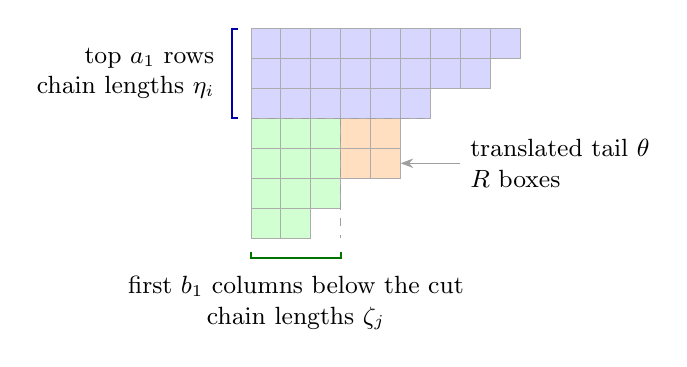
\begin{tikzpicture}[x=0.38cm,y=0.38cm,font=\small]
  \foreach \row/\length in {1/9,2/8,3/6,4/5,5/5,6/3,7/2}{
    \foreach \col in {1,...,\length}{
      \ifnum\row<4
        \fill[blue!16] (\col-1,-\row+1) rectangle (\col,-\row);
      \else
        \ifnum\col<4
          \fill[green!18] (\col-1,-\row+1) rectangle (\col,-\row);
        \else
          \fill[orange!25] (\col-1,-\row+1) rectangle (\col,-\row);
        \fi
      \fi
      \draw[gray!65,line width=0.35pt]
        (\col-1,-\row+1) rectangle (\col,-\row);
    }
  }
  \draw[blue!65!black,line width=0.7pt]
    (-0.45,0)--(-0.65,0)--(-0.65,-3)--(-0.45,-3);
  \node[anchor=east,align=right] at (-0.9,-1.5)
    {top $a_1$ rows\\chain lengths $\eta_i$};
  \draw[green!45!black,line width=0.7pt]
    (0,-7.45)--(0,-7.65)--(3,-7.65)--(3,-7.45);
  \node[anchor=north,align=center] at (1.5,-7.95)
    {first $b_1$ columns below the cut\\chain lengths $\zeta_j$};
  \node[anchor=west,align=left] (tail) at (7,-4.5)
    {translated tail $\theta$\\$R$ boxes};
  \draw[-{Stealth[length=1.6mm]},gray!75] (tail.west)--(5,-4.5);
  \draw[dashed,gray!75] (0,-3)--(6,-3);
  \draw[dashed,gray!75] (3,-3)--(3,-7);
\end{tikzpicture}

\caption{The chain decomposition, shown schematically. The top $a_1$
rows are taken first; the column chains contain only the boxes below
those rows. The remaining lower-right region is a translated straight
diagram $\theta$. Thus the row chains, lower-column chains, and tail
are disjoint, and their sizes sum to $n$. The cut is schematic; the
asymptotic threshold is defined in the text.}
\label{fig:hybrid-chains}
\end{figure}

Every tail cell pays the cap $v_d\log n$, since both of its full
line lengths are below $T$. In a top row, replacing the maximum
of the full row and column lengths by the row length can change
the contribution only in the first $b_1$ columns, at most $a_1b_1$
cells. This has total cost $O(c_d a_1b_1\log(en))$.
Below the top rows, in a long column the maximum is its full
column height. Replacing that height $\zeta_j+a_1$ by its chain
length $\zeta_j$ changes the logarithmic sum by at most
\[
 \zeta_j\log(1+a_1/\zeta_j)\le a_1
\]
for each nonempty chain. Thus the chain contribution is
$c_d\sum_l l\log(n/l)$ up to the same stated error.
Finally $\sum_l l\log(n/l)=G+M\log(n/M)$ and
$M\log(n/M)\le R$. We have proved
\begin{equation}\label{rec:hybrid-arm-weight}
 \mathcal D_d(\lambda)
 =c_dG+v_dR\log n+O(c_d(R+D_0^2\log(en))).
\end{equation}

We also need a hook-product bound for an arbitrary diagram
$\mu\vdash L$, $L\le n$, using these same values of $a_1,b_1$.
Let $l$ be its top-row and lower-column chain lengths, and let
$\vartheta$ be its translated residual diagram of size $q$.
Then
\begin{equation}\label{rec:hybrid-arm-hook}
 D_\mu\ge\frac{L!D_\vartheta}{q!\prod_l l!}
             \exp\{-C(q+D_0^2\log^2(en))\}.
\end{equation}
Here is the hook comparison in detail. Tail hooks are exactly those
of $\vartheta$. On a top row, compare each hook with the baseline
number of cells remaining in that row, including the current cell.
Cells in the first $b_1$ columns cost at most
$O(a_1b_1\log(en))$ altogether. In the other columns, the extra
leg has at most $a_1$ boxes in the top region plus the height of the
corresponding tail column. The first addition costs
$O(a_1\log(en))$ per row by the harmonic sum; the two additions can
be separated using $\log(1+x+y)\le\log(1+x)+\log(1+y)$.

Let the tail have width $w$ and nonincreasing column heights
$h_1,\ldots,h_w$, of sum $q$. If $q>0$, every top row extends at
least through column $b_1+w$, so the tail addition for that row
is bounded by
\[
 \sum_{t=1}^w\log\left(1+\frac{h_t}{w-t+1}\right).
\]
When $w\le D_0\log(en)$, there are at most $a_1w$ affected top-row
cells, each costing at most $\log(en)$, for a total
$O(D_0^2\log^2(en))$. When $w>D_0\log(en)$, use
\[
 \sum_{t=1}^w\frac{h_t}{w-t+1}
 \le \frac{2q}{w}
       +\frac{2q}{w}\sum_{r=1}^{\lceil w/2\rceil}\frac1r
 =O\!\left(\frac q w\log(en)\right).
\]
For the first half of the sum the denominators are at least $w/2$;
for the second half monotonicity gives $h_t\le2q/w$.
After multiplication by the at most $a_1$ top rows, this is $O(q)$.

For the lower-column chains compare hooks with the number of
remaining cells in their column. The extra arm has at most $b_1$
boxes in the left region plus the appropriate tail row length.
The $b_1$ addition has total cost $O(b_1^2\log(en))$.
The tail addition has the identical bound with width and height
interchanged: every left column extends through the tail's rows,
and its row lengths are nonincreasing with sum $q$.
If $q=0$, both tail-addition terms are absent.
The resulting total logarithmic inflation over the product
$(q!/D_\vartheta)\prod_l l!$ is
$O(q+D_0^2\log^2(en))$, proving
\eqref{rec:hybrid-arm-hook}.

At the parent, every hook of $\theta$ is at most
$2n^{1-\gamma_d}$, because all its full row and column lengths
are below the threshold. Therefore
$D_\theta/R!\ge(2n^{1-\gamma_d})^{-R}$.
Also $(n)_R\ge(n/e)^R$ and factorial estimates give
$\log(M!/\prod_l l!)=G+O(D_0\log(en))$.
Applying \eqref{rec:hybrid-arm-hook} yields
\begin{equation}\label{rec:hybrid-arm-dimension}
 \log D_\lambda\ge
 G+\gamma_dR\log n-O(R+D_0^2\log^2(en)),
 \qquad G+R\log n\ge k/2 .
\end{equation}
For the second assertion, if $M>0$ and $l_{\max}$ is the largest
chain length, $-\log x\ge1-x$ gives
\[
 G\ge M-\frac{\sum_l l^2}{M}\ge M-l_{\max}.
\]
Every top chain has length at most $\lambda_1=n-k$, and every
lower-column chain has length at most $\lambda'_1\le n/2$.
Consequently
$G+R\ge n-l_{\max}\ge\min(k,n/2)\ge k/2$.
If $M=0$ the same inequality is immediate from $R=n$.
For sufficiently large $d$, $\log n\ge1$, proving the displayed
version.

\subsection{Color multiplicities and the marked trace}

The arm comparison has expressed the parent budget in terms of $G$
and $R$, and~\eqref{rec:hybrid-arm-dimension} supplies its dimension
scale. To apply~\eqref{rec:hybrid-two-strip}, we still need the local
copy counts, the positive trace with distinct markers, the child
diagram costs, and the color angle. We establish them in that order.

Let $\mathcal H$ be the space of configurations of $R$ distinctly
labeled even markers and signed colors in
$\mathbb C^{a_1}\oplus\mathbb C^{b_1}$. Every marker is used exactly
once. Thus $\mathcal H$ is the orthogonal sum, over the ordered
marker-position tuples, of the signed tensor spaces on the remaining
$M$ sites. The compact group $K=U(a_1)\times U(b_1)$ acts only on
colors; zero factors are omitted.  The selected global type is the
irreducible representation
\[
 \begin{gathered}
 \pi=\pi_{(\eta,\zeta)}:K\longrightarrow
 U(\mathcal U_{\eta,\zeta}),\\
 \mathcal U_{\eta,\zeta}
 =\mathbf S_\eta(\mathbb C^{a_1})
    \otimes\mathbf S_\zeta(\mathbb C^{b_1}),
 \end{gathered}
\]
where the carrier factor belonging to a zero group factor is also
omitted.  Its carrier action extends polynomially to the invertible
parity-preserving block matrices.  Take $S$ to be the full compact
$\pi$-isotypic projection on $\mathcal H$, including all multiplicity
copies. No additional projection is put on the marker labels.

Indeed, by fixing the even, odd, and marker site pattern and then
inducing, Schur--Weyl duality identifies this color isotype on the
permutation side with induction from the Specht factors
$V_\eta,V_{\zeta^{\mathsf t}}$, with the markers fixed pointwise.
Stacking $\zeta^{\mathsf t}$ below $\eta$ gives precisely the
unmarked hook subdiagram. Its Littlewood--Richardson coefficient
is at least one: the skew part below $\eta$ is a translated straight
diagram with its row-constant Littlewood--Richardson tableau.
Adding the $R$ ordered markers by branching then gives at least
$f^{\lambda/(\text{unmarked hook})}=D_\theta$ copies of $V_\lambda$.
The compact carrier dimension can only increase this multiplicity,
so in \eqref{rec:hybrid-two-strip} we may take
$L_\lambda=D_\theta$. Separating the entry sets in the chains and
the tail of a standard tableau gives
\begin{equation}\label{s:hybrid-global-marker-multiplicity}
 \frac{D_\lambda}{L_\lambda}
 \le \binom nR\frac{M!}{\prod_h l_h!}
 \le \binom nR e^G.
\end{equation}
The last inequality is the elementary multinomial entropy bound.

In each row include both the local permutation isotype $\mu_i$
and local color isotype $(\eta^{(i)},\zeta^{(i)})$ in $E_\alpha$; use
$(\nu_j,\eta^{[j]},\zeta^{[j]})$ in each column for $F_\beta$.
The superscripts $(i)$ and $[j]$ distinguish row and column
partitions; subscripts denote their parts. Local color projectors
commute with local permutations. They also commute with the global color projection
because they commute with every element of their local color
group, including the corresponding factor of every diagonal global
rotation. Thus these projections have all the commutations needed
in \eqref{rec:hybrid-two-strip}.
Their degrees fix the marker counts
\[
 x_i=b-|\eta^{(i)}|-|\zeta^{(i)}|,\qquad
 y_j=a-|\eta^{[j]}|-|\zeta^{[j]}|,\qquad
 \sum_i x_i=\sum_jy_j=R.
\]
Only nonnegative counts contribute. For $M_i=b-x_i$ define
\[
 G_i=\sum_{l\ {\rm in}\ \eta^{(i)},\zeta^{(i)}}l\log(M_i/l),
 \qquad G_H=\sum_iG_i,
\]
and define $G'_j,G_V$ analogously in columns. Empty entropies are zero.

We need the local multiplicity with one fixed assignment of marker
labels to a row, while their positions within that row still vary.
The unmarked permutation shapes $\rho\vdash M_i$ have coefficients
$c_{\eta^{(i)},(\zeta^{(i)})^{\mathsf t}}^\rho$. The full local multiplicity
of $\mu_i$ is therefore
\begin{equation}\label{s:hybrid-local-marker-multiplicity}
 \operatorname{mult}_i
 =(\dim\eta^{(i)})(\dim\zeta^{(i)})
   \sum_{\rho\subseteq\mu_i}
    c_{\eta^{(i)},(\zeta^{(i)})^{\mathsf t}}^\rho f^{\mu_i/\rho}.
\end{equation}
Here the two dimensions are compact-group carrier dimensions, and
the sum includes only shapes with nonzero coefficient.

For clarity, we record the size bounds used in this sum. Every such
$\rho$ contains $\eta^{(i)}$ and $(\zeta^{(i)})^{\mathsf t}$ and lies in the
$(a_1,b_1)$ hook. For the latter assertion use a Littlewood--Richardson
tableau of $\rho/(\zeta^{(i)})^{\mathsf t}$ with content $\eta^{(i)}$.
Beyond column $b_1$ its columns have at most $a_1$ boxes, by column
strictness. Let $l^0$ be the vector of its top-row and lower-column
chain lengths, padded by zeros. Its top counts dominate the parts
of $\eta^{(i)}$, while the deficit of each lower-column count from the
corresponding part of $\zeta^{(i)}$ is at most $a_1$. Since the two
vectors have the same total $M_i$, their total absolute discrepancy
is at most $2a_1b_1$. It follows that
\begin{equation}\label{s:hybrid-local-chain-entropy}
 \sum_h l_h^0\log(M_i/l_h^0)
       =G_i+O(D_0^2\log(en)).
\end{equation}
One may bound the entropy change per changed integer unit by
$O(\log(en))$, including the transition between zero and one.

The same tableau argument bounds the coefficient in
\eqref{s:hybrid-local-marker-multiplicity}. The top $a_1$ rows of
$\rho$ contain at least $|\eta^{(i)}|$ boxes, and at most $a_1b_1$
of those belong to the base shape $(\zeta^{(i)})^{\mathsf t}$.
Thus at most $a_1b_1$ boxes of the skew tableau lie below the top
region. In the top region, a weakly increasing row is specified by
its counts of the at most $a_1$ letters, giving at most
$(n+1)^{a_1^2}$ choices. Below it there are at most
$\max(1,a_1)^{a_1b_1}$ choices. The number of possible hook shapes
$\rho$ is at most $(n+1)^{a_1+b_1}$, and the compact carrier
dimensions are $e^{O(D_0^2\log(en))}$ by the Weyl dimension formula.
All these factors therefore fit that exponential bound. In particular,
\eqref{rec:hybrid-arm-hook} and
\eqref{s:hybrid-local-chain-entropy} give
\begin{equation}\label{s:hybrid-unmarked-dimension}
 \log D_\rho\ge G_i-O(D_0^2\log^2(en)).
\end{equation}

For each contributing $\rho\subseteq\mu_i$, let $l_{ih}$ be the
full chain lengths of $\mu_i$, and let $l^0_{ih}$ be those of
$\rho$. Write
\[
 e_{ih}=l_{ih}-l^0_{ih}\ge0,\qquad
 K_i(\rho)=\sum_h\log\binom{l_{ih}}{e_{ih}}.
\]
If the tail of $\mu_i$ has shape $\theta_i$ and size $q_i$, then
$q_i+\sum_he_{ih}=x_i$. Separating the entries in its tail and
chain extensions yields
\[
 f^{\mu_i/\rho}\le
       \frac{x_i!D_{\theta_i}}{q_i!\prod_he_{ih}!}.
\]
Dividing by \eqref{rec:hybrid-arm-hook}, with $L=b$, leaves
$x_i!\prod_hl_{ih}!/(b!\prod_he_{ih}!)$ times
$e^{O(x_i+D_0^2\log^2(en))}$. Factor out the chain binomials and
use \eqref{s:hybrid-local-chain-entropy} to obtain
\begin{equation}\label{s:hybrid-local-ratio}
 \frac{\operatorname{mult}_i}{D_{\mu_i}}
 \le\binom b{x_i}^{-1}
       \exp\{K_i-G_i+O(x_i+D_0^2\log^2(en))\},
\end{equation}
where, once and for all, choose a contributing $\rho_i$ maximizing
$K_i(\rho)$ and set $K_i=K_i(\rho_i)$.
The identity behind the entropy term is
$\prod_h(l^0_{ih})!/M_i!$ after extracting the inverse binomial;
factorial errors and the sum in
\eqref{s:hybrid-local-marker-multiplicity} have the stated size.
Zero local spaces can be discarded.

\paragraph{The marked trace endpoint.}
In a diagonal block of $B_\beta^{2p}A_\alpha^{2p}$, each marker's
intermediate position must equal its starting position: a horizontal
move and a vertical move cannot undo each other's coordinate changes.
Fix one such marker-position tuple. In a column, restricting the
positive group-algebra coefficients to its pointwise marker
stabilizer $S_{a-y_j}$ gives a positive element with regular trace
$T_a^{\nu_j}(p)/(a)_{y_j}$. On a stabilizer irreducible $\rho$,
its operator norm is at most this regular trace divided by $D_\rho$.
On the fixed local color type the occurring $\rho$ satisfy the
column version of \eqref{s:hybrid-unmarked-dimension}.
Consequently the vertical diagonal block has norm at most
\[
 (e/a)^R
 \exp\{-G_V+O(bD_0^2\log^2(en))\}
 \prod_jT_a^{\nu_j}(p).
\]
This holds uniformly over the marker positions; blocks with
incompatible counts are zero. Fixed graded reordering into column
order makes the product over columns literal, without changing
the norm or the marker fibers.

Both diagonal compressions are positive. After applying the vertical
norm bound we may sum the horizontal diagonal traces, which gives
the full horizontal trace. There are $R!/\prod_i x_i!$ ways to
assign the distinct marker labels to rows, and hence
\[
 \Tr_{\mathcal H}A_\alpha^{2p}
 =\frac{R!}{\prod_i x_i!}
       \prod_i\left(\frac{\operatorname{mult}_i}{D_{\mu_i}}
                         T_b^{\mu_i}(p)\right).
\]
Using \eqref{s:hybrid-local-ratio}, the remaining binomial and
position factors, including \eqref{s:hybrid-global-marker-multiplicity},
are bounded by
\[
 \binom nR(e/a)^R
       \frac{R!}{\prod_i x_i!}\prod_i\binom b{x_i}^{-1}
 \le \binom nR R!(e/a)^R(e/b)^R
 \le e^{2R}.
\]
Thus the normalized trace endpoint obeys
\begin{equation}\label{rec:hybrid-marked-trace}
 \begin{split}
 \log\left(\frac{D_\lambda}{L_\lambda}
           \Tr_{\mathcal H}(B_\beta^{2p}A_\alpha^{2p})\right)
 \le{}&\sum_{\rm children}\log T
       +G-G_H-G_V+\sum_iK_i\\
     &+O(R+(a+b)D_0^2\log^2(en)).
 \end{split}
\end{equation}

\paragraph{Charging the child diagrams.}
We next compare the child diagram budgets with the chain entropies.
Keep the maximizing shapes $\rho_i$ chosen in
\eqref{s:hybrid-local-ratio}. Call a horizontal chain $(i,h)$ good
if $l_{ih}\ge b^{1-\alpha_0}$, where
$\alpha_0=v_*/(4c_*)$, and define the number of good extensions by
\[
 e_{\rm good}=\sum_{\substack{i,h\\ l_{ih}\ge b^{1-\alpha_0}}}e_{ih}.
\]
This counts horizontal extension boxes only, so
$0\le e_{\rm good}\le R$.

The $l^0_{ih}$ unmarked boxes in this chain each see a full row or
column length in $\mu_i$ at least $l_{ih}\ge l^0_{ih}$.
Their contribution to $\mathcal D_{\log_2 b}(\mu_i)$ is at most
$c_{\log_2 b}\sum_hl^0_{ih}\log(b/l^0_{ih})$. By
\eqref{s:hybrid-local-chain-entropy} and
$M_i\log(b/M_i)\le x_i$, this is
$c_{\log_2 b}G_i+O(x_i+D_0^2\log(en))$.
Charge the remaining $x_i$ boxes by the cap
$v_{\log_2 b}\log b$. For a good extension box the actual charge
is at most
$c_{\log_2 b}\alpha_0\log b\le(v_*/2)\log b$,
since $c_{\log_2 b}\le2c_*$. The cap is at least $v_*\log b$,
so each such box saves at least $(v_*/2)\log b$.
In columns choose any compatible unmarked shape and make the same
estimate, discarding its extension savings.

Set
$\bar c=\max(c_{\lfloor d/2\rfloor},c_{\lceil d/2\rceil})$ and
$\bar v=\max(v_{\lfloor d/2\rfloor},v_{\lceil d/2\rceil})$.
The marker counts sum to $R$ on each axis and
$\log a+\log b=\log n$. Therefore
\begin{equation}\label{rec:hybrid-child-diagram}
 \sum_{\rm children}\mathcal D_{d_i}(\mu_i)
 \le\bar c(G_H+G_V)+\bar vR\log n
   -(v_*/2)e_{\rm good}\log m
   +O(R+(a+b)D_0^2\log(en)).
\end{equation}

It remains to bound the $K_i$ costs of the extensions.
We may restrict to profile pairs with nonzero angle, since the other
pairs contribute zero to \eqref{rec:hybrid-two-strip}.
We first show that the total length $U_{\rm bad}$ of bad horizontal
chains is at most $2k$, for all sufficiently large $d$.
If $a_1=0$, then $\lambda_1<n^{1-\gamma_d}\le n/2$ and hence
$k\ge n/2$; the total of all horizontal chain lengths is at most
$n\le2k$.
If $a_1>0$, the nonzero space $E_\alpha S\mathcal H$ contains the
global compact type $(\eta,\zeta)$ inside the tensor product of
the prescribed row types. Its highest weight has first even
coordinate $\eta_1=\lambda_1$. Weights add under the diagonal color
action, and in local type $\eta^{(i)}$ every first weight coordinate is
at most $\eta^{(i)}_1$. Thus
\[
 \lambda_1=\eta_1\le\sum_i\eta^{(i)}_1
                  \le\sum_i\mu_{i,1},\qquad
 \sum_i(b-\mu_{i,1})\le k.
\]
The second inequality uses $\eta^{(i)}\subseteq\rho_i\subseteq\mu_i$.
All chains other than a row's first chain lie below that first row.
If the first chain is itself bad, its length
$\mu_{i,1}<b^{1-\alpha_0}\le b/2$ is at most the same row's
minority $b-\mu_{i,1}$. Summing these two contributions gives
$U_{\rm bad}\le2k$.

For any collection of chains with total length $U$ and total
extension count $z>0$, Vandermonde's identity and the binomial bound
give
\[
 \sum_h\log\binom{l_h}{e_h}
 \le\log\binom Uz\le z\log(eU/z).
\]
For bad chains $U\le2k$ and $z\le R$. Using
$\log x\le\log(d+1)+x/(d+1)$ yields the explicit bound
\[
 K_{\rm bad}\le
 R\log(d+1)+\frac{2ek}{d+1}
 =O(R\log(d+1)+k/d).
\]
Zero extension counts contribute zero.
For good chains $U\le n$ and $z=e_{\rm good}$.
If $e_{\rm good}\ge k n^{-\epsilon}$, the dense hypothesis
$k\ge n^{1-\epsilon}$ gives
\[
 K_{\rm good}\le
 e_{\rm good}\log(en/e_{\rm good})
 \le e_{\rm good}(1+2\epsilon\log n)
 \le (v_*/2)e_{\rm good}\log m
\]
for sufficiently large $d$. The final inequality follows from
$2\epsilon<v_*/4$ and
$\log m\ge(\log n-\log2)/2$.
If $0<e_{\rm good}<k n^{-\epsilon}$, monotonicity of
$z\log(en/z)$ on $[0,n]$ instead gives
$K_{\rm good}=O(k n^{-\epsilon}\log(en))$.
Consequently the $K_i$ terms and the negative term in
\eqref{rec:hybrid-child-diagram} together cost at most
\begin{equation}\label{s:hybrid-extension-cost}
 O\!\left(R\log(d+1)+k/d+k n^{-\epsilon}\log(en)\right).
\end{equation}
All thresholds here depend only on the displayed fixed parameters,
not on the eventual exponent $p$.

The color angle supplies the remaining saving:
\begin{equation}\label{rec:hybrid-color-angle}
 \log w\le-\tfrac12(G-G_H-G_V)
                    +O(R+(a+b)D_0^2\log n),\qquad w\le1.
\end{equation}
If $M=0$, there are no unmarked symbols, $G=G_H=G_V=0$, and
\eqref{rec:hybrid-color-angle} follows from $w\le1$.  Assume $M>0$
for the density and deformation argument that follows.
We first pass from the full local color projections to weight
projections. Let $Q_H,Q_V$ be the products of the specified local
color projections on the rows and columns. Write the additional
permutation-type projections as $E^{\rm perm},F^{\rm perm}$, so
$E_\alpha=Q_HE^{\rm perm}$ and $F_\beta=F^{\rm perm}Q_V$.
They commute within their respective lines and with $S$. Hence
\[
 F_\beta E_\alpha S
   =F^{\rm perm}(Q_V S Q_H)E^{\rm perm},
 \qquad w\le\|Q_V S Q_H\|.
\]
All three color projections preserve marker positions, so this norm
is the maximum of the norms on fixed marker-position fibers.

On one such fiber, let $Q_\tau$ be a local color-type projection,
and let $d_\tau$ be its compact carrier dimension. In every
multiplicity copy choose the highest-weight line and let
$P_\tau^{\rm hw}$ project onto their sum. Normalized Haar averaging
on $K=U(a_1)\times U(b_1)$ gives, with $\rho(g)$ denoting the
local tensor color action,
\[
 Q_\tau=d_\tau\int_K
       \rho(g)P_\tau^{\rm hw}\rho(g)^*\,dg.
\]
The highest-weight lines lie in the torus weight space whose symbol
counts are the parts of $\tau$. If $Z_\tau$ projects onto that
whole weight space, then $P_\tau^{\rm hw}\preceq Z_\tau$. Tensor
these positive inequalities over the rows and over the columns and
apply Lemma~\ref{ten:positive-mixtures}, with middle operator $S$.
It follows that
\[
 \|Q_V S Q_H\|
 \le\left(\prod_{\rm lines}d_\tau\right)^{1/2}
      \sup_{\mathbf g,\mathbf h}
       \|Z_V(\mathbf h)S Z_H(\mathbf g)\|.
\]
Here the rotations are independent on each line. The logarithm of
the prefactor is $O((a+b)D_0^2\log n)$ by the Weyl dimension
formula. This argument applies with either parity dimension zero
by omitting that factor of $K$; it uses no commutation between row
and column projections.

Fix the line rotations in this last supremum. If a row has
$M_i>0$ unmarked sites,
let $\sigma_i$ be the parity-block diagonal density whose entries
are its required symbol counts divided by $M_i$, in the chosen
rotated parity basis. If $M_i=0$,
choose any parity-preserving density of trace one instead; that row
has no tensor factors in the fiber.  Define column densities
$\tau_j$ in the same way, using an arbitrary parity-block trace-one
density when its local unmarked count is zero.
Thus every line density has trace one, including empty lines.
On the row weight space $Z_H(\mathbf g)$ the tensor multiplier $\Sigma$ of the
$\sigma_i^{1/2}$ acts by $e^{-G_H/2}$, and the analogous column
multiplier $\mathcal T$ acts by $e^{-G_V/2}$. In particular,
\[
 Z_V(\mathbf h)S Z_H(\mathbf g)
 =e^{(G_H+G_V)/2}
   Z_V(\mathbf h)\mathcal T S\Sigma Z_H(\mathbf g).
\]
Thus the rotated weight-space overlap is at most
$e^{(G_H+G_V)/2}\|\mathcal T S\Sigma\|$.
For the global compact projection use the deformed formula
with $\bar\tau=b^{-1}\sum_j\tau_j$,
$\bar\sigma=a^{-1}\sum_i\sigma_i$, and a real scalar regularizer
$\varepsilon_{\rm reg}>0$.  For an invertible parity-preserving block
matrix $A$, the polynomial tensor action
$\rho(A)=A^{\otimes M}$ acts on the whole color tensor fiber, while
$\pi(A)$ acts on the selected carrier $\mathcal U_{\eta,\zeta}$.
The restriction of $S$ to this fiber is the full compact
$\pi$-isotypic projection. Put
$A_0=(\bar\tau+\varepsilon_{\rm reg}I)^{-1/2}$.
With $dU$ denoting normalized Haar measure
on $K$, apply Lemma~\ref{s:compact-coefficient-extraction} with carrier
matrix $\pi(A_0)^{-1}$, and multiply its tensor action on the left by
$\rho(A_0)$. The formula is
\[
 \begin{gathered}
 S=(\dim\pi)\int_K
 \Tr(\pi(U)^*\pi(A_0)^{-1})\,\rho(A_0U)\,dU.
 \end{gathered}
\]
To bound the trace coefficient, put
\[
 H=\bar\tau+\varepsilon_{\rm reg}I,\qquad
 t=\operatorname{Tr}H=1+\varepsilon_{\rm reg}(a_1+b_1),\qquad
 D=H/t.
\]
Since $M>0$, the total color dimension $a_1+b_1$ is positive,
and $D$ is a trace-one parity-preserving density. Apply
\eqref{eq:signed-carrier-density-upper} with parity dimensions
$a_1,b_1$ and partitions $\eta,\zeta$. Their total degree is $M$
and their entropy is $G$, so $\|\pi(D)\|\le e^{-G}$.
Polynomial homogeneity and positivity give
\[
 \begin{aligned}
 \pi(A_0)^{-1}&=\pi(H^{1/2})=t^{M/2}\pi(D)^{1/2},\\
 \|\pi(A_0)^{-1}\|
       &\le(1+\varepsilon_{\rm reg}(a_1+b_1))^{M/2}e^{-G/2}.
 \end{aligned}
\]
Here the square-root identity follows by diagonalizing $D$ within
its parity blocks. An absent block contributes the trivial carrier
factor and degree zero. Since $\pi(U)$ is unitary, the absolute
trace coefficient is at most $\dim\pi$ times this norm, in addition
to the $\dim\pi$ outside the integral.
For the site factor $\tau_j^{1/2}A_0U\sigma_i^{1/2}$, the squared
Hilbert--Schmidt norms have full-grid mean
\[
 \Tr(A_0\bar\tau A_0\,U\bar\sigma U^*)\le1,
\]
because $A_0\bar\tau A_0\le I$ and $\Tr\bar\sigma=1$.
Thus on the $M$ unmarked sites the product of the site norms is at most
$(n/M)^{M/2}\le e^{R/2}$.  Let $\varepsilon_{\rm reg}$ decrease to zero.
Including the carrier dimensions proves
\eqref{rec:hybrid-color-angle}.

\begin{proof}[Completion of Theorem~\ref{rec:hybrid-main}]
The number $J$ of profile pairs in this application satisfies
\[
 \log J=O\!\left(n^{3/4}+(a+b)D_0\log(en)\right).
\]
Indeed the permutation partitions contribute
$O(a\sqrt b+b\sqrt a)=O(n^{3/4})$ to this logarithm. Every local
compact type is specified by at most $a_1+b_1$ nonnegative parts,
each at most $n$, giving the second term over all lines. Marker
counts are fixed by the local color degrees and introduce no
additional profile choices.

Set $\Delta G=G-G_H-G_V$. Combining
\eqref{rec:hybrid-marked-trace},
\eqref{rec:hybrid-child-diagram},
\eqref{s:hybrid-extension-cost}, and
\eqref{rec:hybrid-color-angle} in
\eqref{rec:hybrid-two-strip}, then subtracting
\eqref{rec:hybrid-arm-weight}, gives
\[
 \begin{split}
 \log T_n^\lambda(p)-\mathcal D_d(\lambda)
 \le{}&(1-\bar c)\Delta G-(p_0-1)(\Delta G)_+\\
 &-(c_d-\bar c)G-(v_d-\bar v)R\log n\\
 &+O_{p_0}\!\left(R\log(d+1)+k/d\right).
 \end{split}
\]
To obtain this error, use $k\ge n^{1-\epsilon}$,
$D_0=O(n^{0.01})$, and $a+b=O(\sqrt n)$. The terms
$(a+b)D_0^2\log^2(en)$, $\log J$, and
$kn^{-\epsilon}\log(en)$ are all $o(k/d)$.
The angle is bounded both by its exponential estimate and by one;
therefore its main term is $-(p_0-1)(\Delta G)_+$, with the stated
$O_{p_0}$ error. No factor in this error depends on the final
choice of $p$.

The first line of the display is nonpositive. If $\Delta G\le0$,
use $1-\bar c>0$; if $\Delta G>0$, use
$1-\bar c-(p_0-1)<0$.
Let $Q=G+R\log n$. By \eqref{rec:hybrid-arm-dimension},
$Q\ge k/2$, and
\[
 R\log(d+1)+k/d
 \le C Q\,\frac{\log(d+1)}d.
\]
The balanced parameter increments satisfy
$c_d-\bar c=v_d-\bar v\ge c d^{-1/3}$.
Their negative contribution is at most $-cd^{-1/3}Q$ and absorbs
the error for sufficiently large $d$. This proves the dense
diagram induction.

For its comparison with dimension, put
$Q_\gamma=G+\gamma_dR\log n$. The fixed parameters give
$\gamma_d\ge10/10001>0$, and $\gamma_d<1$, so
$Q_\gamma\ge cQ\ge ck$.
Moreover $R=o(Q_\gamma)$ uniformly, because
$Q_\gamma\ge\gamma_dR\log n$, and
$D_0^2\log^2(en)=o(Q_\gamma)$ in the dense range. Thus
\eqref{rec:hybrid-arm-weight} and
\eqref{rec:hybrid-arm-dimension} give
\[
 \mathcal D_d(\lambda)=c_dQ_\gamma+o(Q_\gamma),
 \qquad
 \log D_\lambda\ge Q_\gamma-o(Q_\gamma).
\]
The fixed parameter bounds, in particular $c_d<0.011$, prove
$\mathcal D_d(\lambda)\le\frac14\log D_\lambda$ and
$\log D_\lambda\ge ck$ for all sufficiently large $d$.  This
comparison used only the stated height bound and the diagram estimates,
so it also applies to zero blocks in the theorem's domain.
The other levels were covered by the level induction. All thresholds
are chosen before the finite-base exponent $p$.

Choose the finite-base exponent using \eqref{rec:hybrid-explicit-base}.

In the dense range $\|B_n\|^{2p}\le D_\lambda^{-3/4}$ and
$T_n^\lambda(p)\le D_\lambda^{1/4}$.  Thus
$T_n^\lambda(4p)\le D_\lambda^{-2}$.
In the other range $T_n^\lambda(p)\le n^{-k}$, whence
$\|B_n\|^{2p}\le D_\lambda^{-1}n^{-k}$ and
$T_n^\lambda(4p)\le D_\lambda^{-3}n^{-4k}$.
Consequently exactly $4p$ sweeps suffice:
Lemma~\ref{lem:schatten}, with $r=s=4p$, gives
\begin{equation}\label{rec:hybrid-exact-completion}
 \|B_n^{4p}|_{\mathbf1^\perp}\|_{\HS,\mathrm{reg}}^2
 \le\sum_{\lambda\ne(n)}T_n^\lambda(4p)=o(1).
\end{equation}
The dense sum tends to zero because $k\ge n^{1-\epsilon}$ and
dimensions dominate the partition count; the remaining sum is
bounded by $\sum_{k\ge1}e^{O(\sqrt k)}n^{-4k}$.
Thus $4pd$ physical shuffles suffice for all sufficiently large $d$.
\end{proof}

\begingroup
\raggedright
\setlength{\bibsep}{3pt}
\interlinepenalty=10000
\bibliographystyle{plainnat}
\bibliography{references}
\endgroup
\end{document}
